% Options for packages loaded elsewhere
\PassOptionsToPackage{unicode}{hyperref}
\PassOptionsToPackage{hyphens}{url}
\PassOptionsToPackage{dvipsnames,svgnames*,x11names*}{xcolor}
%
\documentclass[
]{krantz}
\usepackage{lmodern}
\usepackage{amssymb,amsmath}
\usepackage{ifxetex,ifluatex}
\ifnum 0\ifxetex 1\fi\ifluatex 1\fi=0 % if pdftex
  \usepackage[T1]{fontenc}
  \usepackage[utf8]{inputenc}
  \usepackage{textcomp} % provide euro and other symbols
\else % if luatex or xetex
  \usepackage{unicode-math}
  \defaultfontfeatures{Scale=MatchLowercase}
  \defaultfontfeatures[\rmfamily]{Ligatures=TeX,Scale=1}
\fi
% Use upquote if available, for straight quotes in verbatim environments
\IfFileExists{upquote.sty}{\usepackage{upquote}}{}
\IfFileExists{microtype.sty}{% use microtype if available
  \usepackage[]{microtype}
  \UseMicrotypeSet[protrusion]{basicmath} % disable protrusion for tt fonts
}{}
\makeatletter
\@ifundefined{KOMAClassName}{% if non-KOMA class
  \IfFileExists{parskip.sty}{%
    \usepackage{parskip}
  }{% else
    \setlength{\parindent}{0pt}
    \setlength{\parskip}{6pt plus 2pt minus 1pt}}
}{% if KOMA class
  \KOMAoptions{parskip=half}}
\makeatother
\usepackage{xcolor}
\IfFileExists{xurl.sty}{\usepackage{xurl}}{} % add URL line breaks if available
\IfFileExists{bookmark.sty}{\usepackage{bookmark}}{\usepackage{hyperref}}
\hypersetup{
  pdftitle={JavaScript for R},
  pdfauthor={John Coene},
  colorlinks=true,
  linkcolor=Maroon,
  filecolor=Maroon,
  citecolor=Blue,
  urlcolor=Blue,
  pdfcreator={LaTeX via pandoc}}
\urlstyle{same} % disable monospaced font for URLs
\usepackage{color}
\usepackage{fancyvrb}
\newcommand{\VerbBar}{|}
\newcommand{\VERB}{\Verb[commandchars=\\\{\}]}
\DefineVerbatimEnvironment{Highlighting}{Verbatim}{commandchars=\\\{\}}
% Add ',fontsize=\small' for more characters per line
\usepackage{framed}
\definecolor{shadecolor}{RGB}{248,248,248}
\newenvironment{Shaded}{\begin{snugshade}}{\end{snugshade}}
\newcommand{\AlertTok}[1]{\textcolor[rgb]{0.33,0.33,0.33}{#1}}
\newcommand{\AnnotationTok}[1]{\textcolor[rgb]{0.37,0.37,0.37}{\textbf{\textit{#1}}}}
\newcommand{\AttributeTok}[1]{\textcolor[rgb]{0.61,0.61,0.61}{#1}}
\newcommand{\BaseNTok}[1]{\textcolor[rgb]{0.06,0.06,0.06}{#1}}
\newcommand{\BuiltInTok}[1]{#1}
\newcommand{\CharTok}[1]{\textcolor[rgb]{0.5,0.5,0.5}{#1}}
\newcommand{\CommentTok}[1]{\textcolor[rgb]{0.37,0.37,0.37}{\textit{#1}}}
\newcommand{\CommentVarTok}[1]{\textcolor[rgb]{0.37,0.37,0.37}{\textbf{\textit{#1}}}}
\newcommand{\ConstantTok}[1]{\textcolor[rgb]{0,0,0}{#1}}
\newcommand{\ControlFlowTok}[1]{\textcolor[rgb]{0.27,0.27,0.27}{\textbf{#1}}}
\newcommand{\DataTypeTok}[1]{\textcolor[rgb]{0.27,0.27,0.27}{#1}}
\newcommand{\DecValTok}[1]{\textcolor[rgb]{0.06,0.06,0.06}{#1}}
\newcommand{\DocumentationTok}[1]{\textcolor[rgb]{0.37,0.37,0.37}{\textbf{\textit{#1}}}}
\newcommand{\ErrorTok}[1]{\textcolor[rgb]{0.14,0.14,0.14}{\textbf{#1}}}
\newcommand{\ExtensionTok}[1]{#1}
\newcommand{\FloatTok}[1]{\textcolor[rgb]{0.06,0.06,0.06}{#1}}
\newcommand{\FunctionTok}[1]{\textcolor[rgb]{0,0,0}{#1}}
\newcommand{\ImportTok}[1]{#1}
\newcommand{\InformationTok}[1]{\textcolor[rgb]{0.37,0.37,0.37}{\textbf{\textit{#1}}}}
\newcommand{\KeywordTok}[1]{\textcolor[rgb]{0.27,0.27,0.27}{\textbf{#1}}}
\newcommand{\NormalTok}[1]{#1}
\newcommand{\OperatorTok}[1]{\textcolor[rgb]{0.43,0.43,0.43}{\textbf{#1}}}
\newcommand{\OtherTok}[1]{\textcolor[rgb]{0.37,0.37,0.37}{#1}}
\newcommand{\PreprocessorTok}[1]{\textcolor[rgb]{0.37,0.37,0.37}{\textit{#1}}}
\newcommand{\RegionMarkerTok}[1]{#1}
\newcommand{\SpecialCharTok}[1]{\textcolor[rgb]{0,0,0}{#1}}
\newcommand{\SpecialStringTok}[1]{\textcolor[rgb]{0.5,0.5,0.5}{#1}}
\newcommand{\StringTok}[1]{\textcolor[rgb]{0.5,0.5,0.5}{#1}}
\newcommand{\VariableTok}[1]{\textcolor[rgb]{0,0,0}{#1}}
\newcommand{\VerbatimStringTok}[1]{\textcolor[rgb]{0.5,0.5,0.5}{#1}}
\newcommand{\WarningTok}[1]{\textcolor[rgb]{0.37,0.37,0.37}{\textbf{\textit{#1}}}}
\usepackage{longtable,booktabs}
% Correct order of tables after \paragraph or \subparagraph
\usepackage{etoolbox}
\makeatletter
\patchcmd\longtable{\par}{\if@noskipsec\mbox{}\fi\par}{}{}
\makeatother
% Allow footnotes in longtable head/foot
\IfFileExists{footnotehyper.sty}{\usepackage{footnotehyper}}{\usepackage{footnote}}
\makesavenoteenv{longtable}
\usepackage{graphicx}
\makeatletter
\def\maxwidth{\ifdim\Gin@nat@width>\linewidth\linewidth\else\Gin@nat@width\fi}
\def\maxheight{\ifdim\Gin@nat@height>\textheight\textheight\else\Gin@nat@height\fi}
\makeatother
% Scale images if necessary, so that they will not overflow the page
% margins by default, and it is still possible to overwrite the defaults
% using explicit options in \includegraphics[width, height, ...]{}
\setkeys{Gin}{width=\maxwidth,height=\maxheight,keepaspectratio}
% Set default figure placement to htbp
\makeatletter
\def\fps@figure{htbp}
\makeatother
\setlength{\emergencystretch}{3em} % prevent overfull lines
\providecommand{\tightlist}{%
  \setlength{\itemsep}{0pt}\setlength{\parskip}{0pt}}
\setcounter{secnumdepth}{5}
\usepackage{booktabs}
\usepackage{longtable}
\usepackage[bf,singlelinecheck=off]{caption}

\usepackage{framed,color}
\definecolor{shadecolor}{RGB}{248,248,248}

\renewcommand{\textfraction}{0.05}
\renewcommand{\topfraction}{0.8}
\renewcommand{\bottomfraction}{0.8}
\renewcommand{\floatpagefraction}{0.75}

\renewenvironment{quote}{\begin{VF}}{\end{VF}}
\let\oldhref\href
\renewcommand{\href}[2]{#2\footnote{\url{#1}}}

\makeatletter
\newenvironment{kframe}{%
\medskip{}
\setlength{\fboxsep}{.8em}
 \def\at@end@of@kframe{}%
 \ifinner\ifhmode%
  \def\at@end@of@kframe{\end{minipage}}%
  \begin{minipage}{\columnwidth}%
 \fi\fi%
 \def\FrameCommand##1{\hskip\@totalleftmargin \hskip-\fboxsep
 \colorbox{shadecolor}{##1}\hskip-\fboxsep
     % There is no \\@totalrightmargin, so:
     \hskip-\linewidth \hskip-\@totalleftmargin \hskip\columnwidth}%
 \MakeFramed {\advance\hsize-\width
   \@totalleftmargin\z@ \linewidth\hsize
   \@setminipage}}%
 {\par\unskip\endMakeFramed%
 \at@end@of@kframe}
\makeatother

\renewenvironment{Shaded}{\begin{kframe}}{\end{kframe}}

\newenvironment{rmdblock}[1]
  {
  \begin{itemize}
  \renewcommand{\labelitemi}{
    \raisebox{-.7\height}[0pt][0pt]{
      {\setkeys{Gin}{width=3em,keepaspectratio}\includegraphics{images/#1}}
    }
  }
  \setlength{\fboxsep}{1em}
  \begin{kframe}
  \item
  }
  {
  \end{kframe}
  \end{itemize}
  }
\newenvironment{rmdnote}
  {\begin{rmdblock}{note}}
  {\end{rmdblock}}
\newenvironment{rmdcaution}
  {\begin{rmdblock}{caution}}
  {\end{rmdblock}}
\newenvironment{rmdimportant}
  {\begin{rmdblock}{important}}
  {\end{rmdblock}}
\newenvironment{rmdtip}
  {\begin{rmdblock}{tip}}
  {\end{rmdblock}}
\newenvironment{rmdwarning}
  {\begin{rmdblock}{warning}}
  {\end{rmdblock}}

\usepackage{makeidx}
\makeindex

\urlstyle{tt}

\usepackage{amsthm}
\makeatletter
\def\thm@space@setup{%
  \thm@preskip=8pt plus 2pt minus 4pt
  \thm@postskip=\thm@preskip
}
\makeatother

\frontmatter
\usepackage[]{natbib}
\bibliographystyle{apalike}

\title{JavaScript for R}
\author{John Coene}
\date{2020-08-23}

\begin{document}
\maketitle

% you may need to leave a few empty pages before the dedication page

%\cleardoublepage\newpage\thispagestyle{empty}\null
%\cleardoublepage\newpage\thispagestyle{empty}\null
%\cleardoublepage\newpage
\thispagestyle{empty}

\begin{center}
To my son,

without whom I should have finished this book two years earlier
%\includegraphics{images/dedication.pdf}
\end{center}

\setlength{\abovedisplayskip}{-5pt}
\setlength{\abovedisplayshortskip}{-5pt}

{
\hypersetup{linkcolor=}
\setcounter{tocdepth}{2}
\tableofcontents
}
\listoftables
\listoffigures
\hypertarget{preface}{%
\chapter*{Preface}\label{preface}}


{Photo by davisco on Unsplash}

The R programming language has seen the integration of many languages; C, C++, Python, to name a few, can be seamlessly embedded into R so one can easily call code written in other languages from the R console. Little known to many, R works just as well with JavaScript---this book delves into the various ways both languages can work together.

The ultimate aim of this work is to demonstrate to the reader the many great benefits one can reap by inviting JavaScript into their data science workflow. In that respect the book is not teaching one JavaScript but rather demonstrates how little JavaScript can greatly support and enhance R code. Therefore focus is on integrating external JavaScript libraries and only limited knowledge of JavaScript is required in order to learn from the book. Moreover, the book focuses on generalisable learnings so the reader can transfer takeaways from the book to solve real-world problems.

Throughout the book several shiny applications and R packages are put together as examples, all of these, along with the code for the entire book can be found on the Github repository: \href{https://github.com/JohnCoene/javascript-for-r}{github.com/JohnCoene/javascript-for-r}.

\hypertarget{premise}{%
\section*{Premise}\label{premise}}


The R programming language has been propelled into web browsers with the introduction of packages such as \href{https://shiny.rstudio.com/}{shiny} \citep{R-shiny} and \href{https://rmarkdown.rstudio.com/}{rmarkdown} \citep{R-rmarkdown} which have greatly improved how R users can communicate complex insights by building interactive web applications and interactive documents. Yet most R developers are not familiar with one of web browsers' core technology: JavaScript. This books aims to remedy to that.

The book is nonetheless not about learning JavaScript, even though it is aimed at R developers with little knowledge of the language. This statement might appear counter-intuitive at first but, we hope, the book gradually reveals just how little JavaScript is actually needed in order to observe immense benefits otherwise locked away from R developers.

Importantly, the focus of the book truly is the integration of JavaScript with R where both languages either actively interact with one another, or where JavaScript enables doing things otherwise not accessible to R users---it is not merely about including JavaScript code that works alongside R.

\hypertarget{book-structure}{%
\section*{Book Structure}\label{book-structure}}


\begin{enumerate}
\def\labelenumi{\arabic{enumi}.}
\item
  The book opens with an introduction to better illustrate its premise, it provides rationales for using JavaScript in conjunction with R which it supports with existing R packages that make use of JavaScript and are available on CRAN. Then it briefly describes concepts essential to understand the rest of the book to ensure the reader can follow along. Finally, this part closes by listing the various methods with which one might make JavaScript work with R.
\item
  We explore existing integrations of JavaScript and R namely by exploring packages to grasp how these tend to work and the interface to JavaScript they provide.
\item
  A sizeable part of the book concerns data visualisation, it plunges into creating interactive outputs with the htmlwidgets package. This opens with a brief overview of how it works and libraries that make great candidates to integrate with the htmlwidgets package. Then a first, admittedly unimpressive, widget is built to look under the hood and observe the inner-workings of such outputs in order to grasp a better understanding of how htmlwidgets work. Next, we tackle a more substantial library that allows drawing arcs between countries on a 3D globe. Then, to demonstrate that such packages are not limited to visualisation and more broadly applies to interactive outputs, a second package is built, one that allows to mimic text being typed on the screen. The last two chapter go into more advanced topics such as security and resizing.
\item
  The fourth part of the book details how JavaScript can work with Shiny. Once the basics out of the way, the second chapter builds the first utility to programmatically display notifications. Then we create a functionality to notify the user when the shiny server is busy running computations. This part of the book ends with an example of custom shiny output for a library that applies filters to images. Finally, shiny and htmlwidgets are (literally) connected by including additional functionalities in interactive visualisations when used with the shiny framework.
\item
  Finally, we look at how one can use some of the more modern JavaScript technologies such as Vue, React, and webpack with R---these can make the use of JavaScript more agile and robust.
\item
  Then the book delves into using JavaScript for computations, namely via the V8 engine and node.js. After a short introduction, chapters will walk the reader through various examples: a fuzzy search, a time format converter, and some basic natural language operations.
\item
  Next the book closes with examples of all the integrations explored previously. This involves recreating (a part of) the plotly package, building an image classifier, adding progress bars to a shiny application, building an app with HTTP cookies and running basic machine learning operations in JavaScript.
\item
  Finally, the book concludes with some noteworthy remarks on where to go next.
\end{enumerate}

\hypertarget{acknowledgement}{%
\section*{Acknowledgement}\label{acknowledgement}}


Many people in the R community have inspired me and provided the knowledge to ultimately write this book, amongst them are \href{https://github.com/ramnathv/}{Ramnath Vaidyanathan} for his amazing work on the htmlwidgets \citep{R-htmlwidgets} package, \href{https://github.com/timelyportfolio}{Kent Russel} from whom I have learned a lot via his work on making Vue and React accessible in R, and \href{https://github.com/cpsievert}{Carson Sievert} for pioneering probably the most popular integration of R and JavaScript with the plotly \citep{R-plotly} package.

\hypertarget{disclaimer}{%
\section*{Disclaimer}\label{disclaimer}}


This book is currently a work in progress.

\mainmatter

\hypertarget{part-basics-roadmap}{%
\part{Basics \& Roadmap}\label{part-basics-roadmap}}

\hypertarget{introduction}{%
\chapter{Introduction}\label{introduction}}

This book starts with a rationale for integrating JavaScript with R and supports it with examples, namely packages that use JavaScript and are available on CRAN. Then, we list the various ways in which one might go about making both languages work together. In the next chapter, we go over prerequisites and a review of concepts fundamental to fully understand the more advanced topics residing in the forthcoming chapters.

\hypertarget{rationale}{%
\section{Rationale}\label{rationale}}

Why blend two languages seemingly so far removed from each other? Well, precisely because they are fundamentally different languages that each have their strengths and weaknesses, combining the two allows making the most of their consolidated advantages and circumvent their respective limitations to produce software altogether better for it.

Nevertheless, a fair reason to use JavaScript might simply be that the thing one wants to achieve in R has already been realised in JavaScript. Why reinvent the wheel when the solution already exists and that it can be made accessible from R? The R package \href{https://github.com/ropensci/lawn}{lawn} \citep{R-lawn} by Ropensci integrates \href{http://turfjs.org/}{turf.js}, a brilliant library for geo-spatial analysis. JavaScript is by no means required to make those computations, they could be rewritten solely in R but that would be vastly more laborious than wrapping the JavaScript API in R as done by the package lawn.

\begin{Shaded}
\begin{Highlighting}[]
\KeywordTok{library}\NormalTok{(lawn)}

\KeywordTok{lawn\_count}\NormalTok{(lawn\_data}\OperatorTok{$}\NormalTok{polygons\_count, lawn\_data}\OperatorTok{$}\NormalTok{points\_count, }\StringTok{"population"}\NormalTok{)}
\end{Highlighting}
\end{Shaded}

\begin{verbatim}
## <FeatureCollection>
##   Bounding box: -112.1 46.6 -112.0 46.6
##   No. features: 2
##   No. points: 20
##   Properties: 
##     values count
## 1 200, 600     2
## 2              0
\end{verbatim}

Another great reason is that JavaScript can do things that R cannot, e.g.: run in the browser. Therefore one cannot natively create interactive visualisations with R. \href{https://plotly-r.com/}{Plotly} \citep{R-plotly} by Carson Sievert packages the \href{https://plot.ly/}{plotly JavaScript library} to let one create interactive visualisations solely from R code.

\begin{Shaded}
\begin{Highlighting}[]
\KeywordTok{library}\NormalTok{(plotly)}

\KeywordTok{plot\_ly}\NormalTok{(diamonds, }\DataTypeTok{x =} \OperatorTok{\textasciitilde{}}\NormalTok{cut, }\DataTypeTok{color =} \OperatorTok{\textasciitilde{}}\NormalTok{clarity)}
\end{Highlighting}
\end{Shaded}

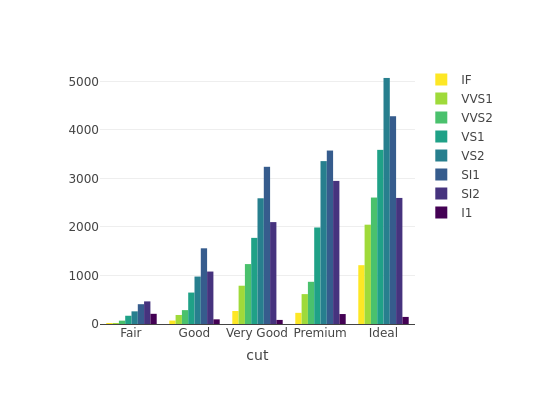
\includegraphics{bookdown_files/figure-latex/unnamed-chunk-2-1.png}

Finally, JavaScript can work together with R to improve how we communicate insights. One of the many ways in which Shiny stands out is that it lets one create web applications solely from R code with no knowledge of HTML, CSS, or JavaScript but that does not mean they can't extend Shiny, quite the contrary. The \href{http://waiter.john-coene.com/}{waiter package} \citep{R-waiter} integrates a variety of JavaScript libraries to display loading screens in Shiny applications.

\begin{Shaded}
\begin{Highlighting}[]
\KeywordTok{library}\NormalTok{(shiny)}
\KeywordTok{library}\NormalTok{(waiter)}

\NormalTok{ui <{-}}\StringTok{ }\KeywordTok{fluidPage}\NormalTok{(}
  \KeywordTok{use\_waiter}\NormalTok{(), }\CommentTok{\# include dependencies}
  \KeywordTok{actionButton}\NormalTok{(}\StringTok{"show"}\NormalTok{, }\StringTok{"Show loading for 3 seconds"}\NormalTok{)}
\NormalTok{)}

\NormalTok{server <{-}}\StringTok{ }\ControlFlowTok{function}\NormalTok{(input, output, session)\{}
  \CommentTok{\# create a waiter}
\NormalTok{  w <{-}}\StringTok{ }\NormalTok{Waiter}\OperatorTok{$}\KeywordTok{new}\NormalTok{()}

  \CommentTok{\# on button click}
  \KeywordTok{observeEvent}\NormalTok{(input}\OperatorTok{$}\NormalTok{show, \{}
\NormalTok{    w}\OperatorTok{$}\KeywordTok{show}\NormalTok{()}
    \KeywordTok{Sys.sleep}\NormalTok{(}\DecValTok{3}\NormalTok{)}
\NormalTok{    w}\OperatorTok{$}\KeywordTok{hide}\NormalTok{()}
\NormalTok{  \})}
\NormalTok{\}}

\KeywordTok{shinyApp}\NormalTok{(ui, server)}
\end{Highlighting}
\end{Shaded}

\begin{figure}
\centering

\includegraphics{images/waiter.png}
\caption{Waiter Output}
\end{figure}

Hopefully this makes a couple of great reasons and alluring examples to entice the reader to persevere with this book.

\hypertarget{methods}{%
\section{Methods}\label{methods}}

Though perhaps not obvious at first, all of the packages used as examples in the previous section interfaced with R very differently. As we'll discover, there many ways in which one can blend JavaScript with R, generally the way to go about it is dictated by the nature of what is to be achieved.

Let's list the methods available to us to blend JavaScript with R before covering them each in-depth in their own respective chapter later in the book.

\hypertarget{v8}{%
\subsection{V8}\label{v8}}

\href{https://github.com/jeroen/v8}{V8} by Jeroen Ooms is an R interface to Google's JavaScript engine. It will let you run JavaScript code directly from R and get the result back, it even comes with an interactive console. This is the way the lawn package used in a previous example internally interfaces with the turf.js library.

\begin{Shaded}
\begin{Highlighting}[]
\KeywordTok{library}\NormalTok{(V8)}
\end{Highlighting}
\end{Shaded}

\begin{verbatim}
## Using V8 engine 6.8.275.32-node.55
\end{verbatim}

\begin{Shaded}
\begin{Highlighting}[]
\NormalTok{ctx <{-}}\StringTok{ }\KeywordTok{v8}\NormalTok{()}

\NormalTok{ctx}\OperatorTok{$}\KeywordTok{eval}\NormalTok{(}\StringTok{"2 + 2"}\NormalTok{) }\CommentTok{\# this is evaluated in JavaScript!}
\end{Highlighting}
\end{Shaded}

\begin{verbatim}
## [1] "4"
\end{verbatim}

\hypertarget{htmlwidgets}{%
\subsection{htmlwidgets}\label{htmlwidgets}}

\href{http://www.htmlwidgets.org/}{htmlwidgets} \citep{R-htmlwidgets} specialises in wrapping JavaScript libraries that generate visual outputs. This is what packages such as plotly, \href{https://rstudio.github.io/DT/}{DT} \citep{R-DT}, \href{http://jkunst.com/highcharter/}{highcharter} \citep{R-highcharter}, and many more use to provide interactive visualisation with R.

It is by far the most popular integration out there, at the time of writing this it has been downloaded nearly 10 million times from CRAN. It will therefore be covered extensively in later chapters.

\hypertarget{shiny}{%
\subsection{Shiny}\label{shiny}}

The Shiny framework allows creating applications accessible from web browsers where JavaScript natively runs, it follows that JavaScript can run \emph{alongside} such applications. Often overlooked though, the two can also work \emph{hand-in-hand} as one can pass data from the R server to the JavaScript front-end and vice versa. This is how the package waiter mentioned previously internally works with R.

\hypertarget{bubble}{%
\subsection{bubble}\label{bubble}}

\href{https://github.com/ColinFay/bubble}{bubble} \citep{R-bubble} by Colin Fay is a more recent R package, still under heady development but very promising: it lets one run \href{https://nodejs.org/en/}{node.js} code in R, comes with an interactive node REPL, the ability to install npm packages, and even an R markdown engine. It's similar to V8 in many ways.

\begin{Shaded}
\begin{Highlighting}[]
\KeywordTok{library}\NormalTok{(bubble)}

\NormalTok{n <{-}}\StringTok{ }\NormalTok{NodeSession}\OperatorTok{$}\KeywordTok{new}\NormalTok{() }

\NormalTok{n}\OperatorTok{$}\KeywordTok{eval}\NormalTok{(}\StringTok{"2 + 2"}\NormalTok{) }\CommentTok{\# this is evaluated in node.js}
\end{Highlighting}
\end{Shaded}

\begin{verbatim}
## 4
\end{verbatim}

\hypertarget{methods-amiss}{%
\section{Methods Amiss}\label{methods-amiss}}

Note that there are also two other prominent ways one can use JavaScript with R that are not covered in this book. The main reason being that they require great knowledge of specific JavaScript libraries, d3.js and React, and while these are themselves advanced uses of JavaScript, their integration with R via the packages listed below is rather straightforward.

\hypertarget{reactr}{%
\subsection{reactR}\label{reactr}}

\href{https://react-r.github.io/reactR/}{ReactR} \citep{R-reactR} is an R package that emulates very well htmlwidgets but specifically for the \href{https://reactjs.org/}{React framework}. Unlike htmlwidgets it is not limited to visual outputs and also provides functions to build inputs, e.g.: a drop-down menu (like \texttt{shiny::selectInput}). The \href{https://glin.github.io/reactable/}{reactable package} \citep{R-reactable} uses reactR to enable building interactive tables solely from R code.

\begin{Shaded}
\begin{Highlighting}[]
\NormalTok{reactable}\OperatorTok{::}\KeywordTok{reactable}\NormalTok{(iris[}\DecValTok{1}\OperatorTok{:}\DecValTok{5}\NormalTok{, ], }\DataTypeTok{showPagination =} \OtherTok{TRUE}\NormalTok{)}
\end{Highlighting}
\end{Shaded}

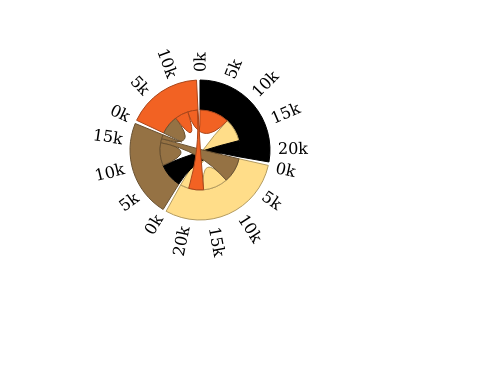
\includegraphics{bookdown_files/figure-latex/unnamed-chunk-5-1.png}

\hypertarget{r2d3}{%
\subsection{r2d3}\label{r2d3}}

\href{https://rstudio.github.io/r2d3/}{r2d3} \citep{R-r2d3} by RStudio is an R package designed specifically to work with \href{https://d3js.org/}{d3.js}. It is similar to htmlwidgets but works rather differently.

\begin{Shaded}
\begin{Highlighting}[]
\CommentTok{\# https://rstudio.github.io/r2d3/articles/gallery/chord/}
\NormalTok{r2d3}\OperatorTok{::}\KeywordTok{r2d3}\NormalTok{(}
  \DataTypeTok{data =} \KeywordTok{matrix}\NormalTok{(}\KeywordTok{round}\NormalTok{(}\KeywordTok{runif}\NormalTok{(}\DecValTok{16}\NormalTok{, }\DecValTok{1}\NormalTok{, }\DecValTok{10000}\NormalTok{)), }\DataTypeTok{ncol =} \DecValTok{4}\NormalTok{, }\DataTypeTok{nrow =} \DecValTok{4}\NormalTok{), }
  \DataTypeTok{script =} \StringTok{"chord.js"}
\NormalTok{)}
\end{Highlighting}
\end{Shaded}

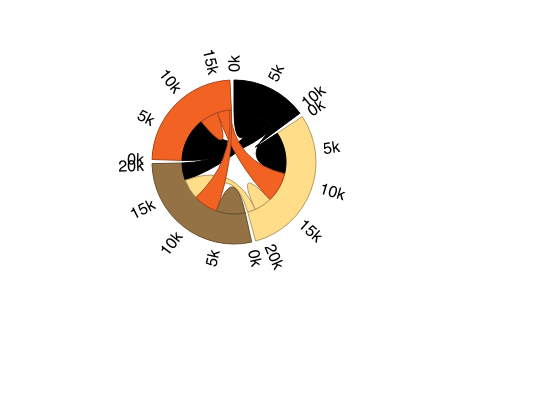
\includegraphics{bookdown_files/figure-latex/unnamed-chunk-6-1.png}

\hypertarget{prerequisites}{%
\chapter{Prerequisites}\label{prerequisites}}

The code contained in the following pages is approachable to readers with basic knowledge of R, but familiarity with package development using \href{https://devtools.r-lib.org/}{devtools} \citep{R-devtools}, the \href{https://shiny.rstudio.com/}{Shiny} framework \citep{R-shiny}, the JSON data format, and JavaScript are essential.

The reason for the former is that some of the ways one builds integrations with JavaScript naturally take the form of R packages. Also, R packages make sharing code, datasets, and anything else R-related extremely convenient, they come with a relatively strict structure, the ability to run unit tests, and much more. These have thus become a core feature of the R ecosystem and therefore are also used extensively in the book as we create several packages. The following section thus runs over the essentials of building a package to ensure everyone can keep up.

Then we briefly go through the JSON data format as it will be used to a great extent to communicate between R and JavaScript. Since both Shiny and JavaScript run in the browser they make for axiomatic companions; we'll therefore use Shiny extensively. Finally, there is an obligatory short introduction to JavaScript.

It is highly recommended to use the freely available \href{https://rstudio.com/products/rstudio/}{RStudio IDE} to follow along as it makes a lot of things easier down the line.

\hypertarget{r-package-development}{%
\section{R Package Development}\label{r-package-development}}

Developing packages used to be notoriously difficult but things have greatly changed in recent years, namely thanks to the devtools \citep{R-devtools}, roxygen2 \citep{R-roxygen2} and more recent \href{https://usethis.r-lib.org/}{usethis} \citep{R-usethis} packages. Devtools is short for ``developer tools,'' it is specifically designed to help creating packages; setting up tests, running checks, building and installing packages, etc. The second provides an all too convenient way to generate the documentation of packages, and usethis, more broadly helps setting up projects, and automating repetitive tasks. Here, we only skim over the fundamentals, there is an entire book by Hadley Wickham called \href{http://r-pkgs.had.co.nz/}{R Packages} solely dedicated to the topic.

Start by installing those packages from CRAN, the roxygen2 package does not need to be explicitly installed as it is a dependency of devtools.

\begin{Shaded}
\begin{Highlighting}[]
\KeywordTok{install.packages}\NormalTok{(}\KeywordTok{c}\NormalTok{(}\StringTok{"devtools"}\NormalTok{, }\StringTok{"usethis"}\NormalTok{))}
\end{Highlighting}
\end{Shaded}

\hypertarget{creating-a-package}{%
\subsection{Creating a Package}\label{creating-a-package}}

There are multiple ways to create a package. One could manually create every file, use the RStudio IDE, or create it from the R console with the usethis \citep{R-usethis} package.

From the RStudio IDE go to \texttt{File\ \textgreater{}\ New\ Project\ \textgreater{}\ New\ Directory\ \textgreater{}\ R\ Package} then select ``R package'' and fill in the small form, namely name the package and specify the directory where it should be created.

\begin{figure}
\centering
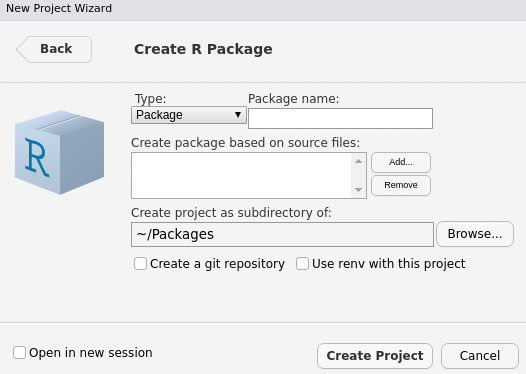
\includegraphics{images/rstudio-create-package.png}
\caption{Package creation wizard}
\end{figure}

But it could be argued that it's actually easier from the R console with the usethis package. The \texttt{create\_package} function takes as first argument the path to create the package. If you run it from RStudio a new project window should open.

\begin{Shaded}
\begin{Highlighting}[]
\CommentTok{\# creates a package named "test" in root of directory.}
\NormalTok{usethis}\OperatorTok{::}\KeywordTok{create\_package}\NormalTok{(}\StringTok{"test"}\NormalTok{)}
\end{Highlighting}
\end{Shaded}

\begin{verbatim}
✔ Creating 'test/'
✔ Setting active project to '/Packages/test'
✔ Creating 'R/'
✔ Writing 'DESCRIPTION'
Package: test
Title: What the Package Does (One Line, Title Case)
Version: 0.0.0.9000
Authors@R (parsed):
    * First Last <first.last@example.com> [aut, cre] (YOUR-ORCID-ID)
Description: What the package does (one paragraph).
License: `use_mit_license()`, `use_gpl3_license()` or friends to
    pick a license
Encoding: UTF-8
LazyData: true
Roxygen: list(markdown = TRUE)
RoxygenNote: 7.1.1.9000
✔ Writing 'NAMESPACE'
✔ Changing working directory to 'test/'
✔ Setting active project to '<no active project>'
\end{verbatim}

\hypertarget{metadata}{%
\subsection{Metadata}\label{metadata}}

Every R package includes a \texttt{DESCRIPTION} file which includes metadata about the package. This includes a range of things like the license defining who can use the package, the name of the package, its dependencies, and more. Below is the default created by the usethis package with \texttt{usethis::create\_package("test")}.

\begin{verbatim}
Package: test
Title: What the Package Does (One Line, Title Case)
Version: 0.0.0.9000
Authors@R: 
    person(given = "First",
           family = "Last",
           role = c("aut", "cre"),
           email = "first.last@example.com",
           comment = c(ORCID = "YOUR-ORCID-ID"))
Description: What the package does (one paragraph).
License: `use_mit_license()`, `use_gpl3_license()` or friends to
    pick a license
Encoding: UTF-8
LazyData: true
Roxygen: list(markdown = TRUE)
RoxygenNote: 7.1.1.9000
\end{verbatim}

Much of this is outside the scope of the book. However, it is good to grasp how dependencies are specified. As packages are generally intended for sharing with others it is important to ensure users of the package meet the dependencies otherwise the package may not work in places. For instance, were we to create a package that relies on one or more functions from the stringr \citep{R-stringr} package we would need to ensure people who install the package actually have it installed on their machine or those functions will not work.

\begin{Shaded}
\begin{Highlighting}[]
\CommentTok{\# R/string.R}
\NormalTok{string\_length <{-}}\StringTok{ }\ControlFlowTok{function}\NormalTok{(string) \{}
\NormalTok{  stringr}\OperatorTok{::}\KeywordTok{str\_length}\NormalTok{(string)}
\NormalTok{\}}
\end{Highlighting}
\end{Shaded}

\begin{rmdnote}
Note that the function is preceded by its namespace with \texttt{::}
(more on this later).
\end{rmdnote}

The \texttt{DESCRIPTION} file does this, it will make sure that the dependencies of the package are met by users who install it. We can specify such dependencies under \texttt{Imports} where we can list packages required separated by a comma.

\begin{verbatim}
Imports:
  stringr,
  dplyr
\end{verbatim}

Then again, the usethis package also allows doing so consistently from the R console, which is great to avoid mishandling the \texttt{DESCRIPTION} file.

\begin{Shaded}
\begin{Highlighting}[]
\CommentTok{\# add stringr under Imports}
\NormalTok{usethis}\OperatorTok{::}\KeywordTok{use\_package}\NormalTok{(}\StringTok{\textquotesingle{}stringr\textquotesingle{}}\NormalTok{)}
\end{Highlighting}
\end{Shaded}

One can also specify another type of dependencies under \texttt{Suggests}, other packages that enhance that enhance the package but are not required to run it. These, unlike package under `Imports' are not automatically installed if missing which can greatly reduce overhead.

\hypertarget{r-code}{%
\subsection{R code}\label{r-code}}

An R package must follow a strict structure. R code must be placed in an \texttt{R/} directory so one should only find \texttt{.R} files in that directory. These files generally contain functions, methods, and R objects.

\begin{Shaded}
\begin{Highlighting}[]
\CommentTok{\# R/add.R}
\NormalTok{string\_length <{-}}\StringTok{ }\ControlFlowTok{function}\NormalTok{(strings) \{}
\NormalTok{  stringr}\OperatorTok{::}\KeywordTok{str\_length}\NormalTok{(strings)}
\NormalTok{\}}
\end{Highlighting}
\end{Shaded}

\hypertarget{documentation}{%
\subsection{Documentation}\label{documentation}}

Documenting packages used to be notoriously complicated but thanks to the package roxygen2 it no longer is the case. The documentation of functions of the package (accessible with \texttt{?}) and datasets that comprise the package reside in separate files in the \texttt{man/} directory. These are \texttt{.Rd} files that use a custom syntax resembling LaTex. The roxygen package eases the creation of these files by turning special comments and tags in \texttt{.R} files into said \texttt{.Rd} files.

Special comments are a standard R comment \texttt{\#} followed by an apostrophe \texttt{\textquotesingle{}}. The first sentence of the documentation is the title of the documentation file while the second is the description.

\begin{Shaded}
\begin{Highlighting}[]
\CommentTok{\#\textquotesingle{} Strings Length}
\CommentTok{\#\textquotesingle{} }
\CommentTok{\#\textquotesingle{} Returns the number of characters in strings. }
\NormalTok{string\_length <{-}}\StringTok{ }\ControlFlowTok{function}\NormalTok{(strings) \{}
\NormalTok{  stringr}\OperatorTok{::}\KeywordTok{str\_length}\NormalTok{(strings)}
\NormalTok{\}}
\end{Highlighting}
\end{Shaded}

There are a plethora of roxygen2 tags to further document different sections, below we use two different tags to document the parameters and give an example.

\begin{Shaded}
\begin{Highlighting}[]
\CommentTok{\#\textquotesingle{} Strings Length}
\CommentTok{\#\textquotesingle{} }
\CommentTok{\#\textquotesingle{} Returns the number of characters in strings. }
\CommentTok{\#\textquotesingle{} }
\CommentTok{\#\textquotesingle{} @param strings A vector of character strings.}
\CommentTok{\#\textquotesingle{} }
\CommentTok{\#\textquotesingle{} @example string\_length(c("hello", "world"))}
\NormalTok{string\_length <{-}}\StringTok{ }\ControlFlowTok{function}\NormalTok{(strings) \{}
\NormalTok{  stringr}\OperatorTok{::}\KeywordTok{str\_length}\NormalTok{(strings)}
\NormalTok{\}}
\end{Highlighting}
\end{Shaded}

As well as generating documentation the roxygen2 package also allows populating the \texttt{NAMESPACE} file. This is an extensive and often confusing topic but for the purpose of this book we'll content with the following: the \texttt{NAMESPACE} includes functions that are \emph{imported} and \emph{exported} by the package.

By default functions that are present in the R files in the \texttt{R/} directory are not exported: they are not accessible outside the package. Therefore the \texttt{string\_length} function defined previously will not be made available to users of the package, only other function within the package will be able to call it. In order to export it we can use the \texttt{@export} tag. This will place the function as exported in the \texttt{NAMESPACE} file.

\begin{Shaded}
\begin{Highlighting}[]
\CommentTok{\#\textquotesingle{} Strings Length}
\CommentTok{\#\textquotesingle{} }
\CommentTok{\#\textquotesingle{} Returns the number of characters in strings. }
\CommentTok{\#\textquotesingle{} }
\CommentTok{\#\textquotesingle{} @param strings A vector of character strings.}
\CommentTok{\#\textquotesingle{} }
\CommentTok{\#\textquotesingle{} @example string\_length(c("hello", "world"))}
\CommentTok{\#\textquotesingle{} }
\CommentTok{\#\textquotesingle{} @export}
\NormalTok{string\_length <{-}}\StringTok{ }\ControlFlowTok{function}\NormalTok{(strings) \{}
\NormalTok{  stringr}\OperatorTok{::}\KeywordTok{str\_length}\NormalTok{(strings)}
\NormalTok{\}}
\end{Highlighting}
\end{Shaded}

There are two ways to use external functions (functions from other R packages), as done thus far in the \texttt{string\_length} function by using the namespace (package name) to call the function: \texttt{stringr::str\_length}. Or by importing the function needed using a roxygen2 tag thereby removing the need for using the namespace.

\begin{Shaded}
\begin{Highlighting}[]
\CommentTok{\#\textquotesingle{} Strings Length}
\CommentTok{\#\textquotesingle{} }
\CommentTok{\#\textquotesingle{} Returns the number of characters in strings. }
\CommentTok{\#\textquotesingle{} }
\CommentTok{\#\textquotesingle{} @param strings A vector of character strings.}
\CommentTok{\#\textquotesingle{} }
\CommentTok{\#\textquotesingle{} @example string\_length(c("hello", "world"))}
\CommentTok{\#\textquotesingle{} }
\CommentTok{\#\textquotesingle{} @importFrom stringr str\_length}
\CommentTok{\#\textquotesingle{} }
\CommentTok{\#\textquotesingle{} @export}
\NormalTok{string\_length <{-}}\StringTok{ }\ControlFlowTok{function}\NormalTok{(strings) \{}
  \KeywordTok{str\_length}\NormalTok{(strings) }\CommentTok{\# namespace removed}
\NormalTok{\}}
\end{Highlighting}
\end{Shaded}

Above we import the function \texttt{str\_length} from the \texttt{stringr} package using the \texttt{importFrom} roxygen2 tag. The first term following the tag is the name of the package wherefrom to import the functions and the following terms are the name of the functions separated by spaces so one can import multiple functions from the same package with, e.g.: \texttt{@importFrom\ stringr\ str\_length\ str\_to\_upper}. If the package uses very many functions from a single package one might also consider importing said package in its entirety with e.g.: \texttt{@import\ stringr}.

Finally, one can actually generate the \texttt{.Rd} documentation files and populate the \texttt{NAMESPACE} with either the \texttt{devtools::document()} function or \texttt{roxygen2::roxygenise()}.

\begin{rmdnote}
Remember to run \texttt{devtools::document()} after changing roxygen2
tags otherwise changes are not actually reflected in the
\texttt{NAMESPACE} and documentation.
\end{rmdnote}

\hypertarget{installed-files}{%
\subsection{Installed files}\label{installed-files}}

Here we tackle the topic of installed files as it will be relevant to much of what the book covers. Installed files are files that are downloaded and copied as-is when users install the package. This directory will therefore come in very handy to store JavaScript files that package will require. These files can be accessed with the \texttt{system.file} function which will look for a file from the root of the \texttt{inst/} directory.

\begin{Shaded}
\begin{Highlighting}[]
\CommentTok{\# return path to \textasciigrave{}inst/dependency.js\textasciigrave{} in \textasciigrave{}myPackage\textasciigrave{}}
\NormalTok{path <{-}}\StringTok{ }\KeywordTok{system.file}\NormalTok{(}\StringTok{"dependency.js"}\NormalTok{, }\DataTypeTok{package =} \StringTok{"myPackage"}\NormalTok{)}
\end{Highlighting}
\end{Shaded}

\hypertarget{build-load-and-install}{%
\subsection{Build, load, and install}\label{build-load-and-install}}

Finally, after generating the documentation of the package with \texttt{devtools::document()} one can install it locally with \texttt{devtools::install()}. This however can take a few seconds too many whilst developing a package as one iterates and regularly tries things; \texttt{devtools::load\_all()} will not install the package but load all the functions and object in the global environment to let you run them.

There is some cyclical nature to developing packages:

\begin{enumerate}
\def\labelenumi{\arabic{enumi}.}
\tightlist
\item
  Write some code
\item
  Run \texttt{devtools::document()} (if documentation tags have changed)
\item
  Run \texttt{devtools::load\_all()}
\item
  Repeat
\end{enumerate}

Note whilst this short guide will help you develop packages good enough for your system it will certainly not pass CRAN checks.

\hypertarget{json}{%
\section{JSON}\label{json}}

JSON (JavaScript Object Notation) is a very popular data \emph{interchange} format with which we will work extensively throughout this book, it is thus crucial that we have a good understanding of it before we plunge into the nitty-gritty. As one might foresee, if we want two languages to work together it is essential that we have a data format that can be understood by both---JSON lets us harmoniously pass data from one to the other. While it is natively supported in JavaScript, it can be graciously handled in R with the \href{https://CRAN.R-project.org/package=jsonlite}{jsonlite package} \citep{R-jsonlite}, in fact it is the serialiser used internally by all the packages we shall explore in this book.

\begin{rmdnote}
``To serialise'' is just jargon for converting data to JSON.
\end{rmdnote}

\hypertarget{serialising}{%
\subsection{Serialising}\label{serialising}}

JSON is to all intents and purposes the equivalent of lists in R; a flexible data format that can store pretty much anything--expect data.frames a structure that does not exist in JavaScript. Below we create a nested list and convert it to JSON with the help of jsonlite, we set \texttt{pretty} to \texttt{TRUE} to add indentation for clearer printing but this is an argument you should omit when writing production code, it will reduce the file size (fewer spaces = smaller file size).

\begin{Shaded}
\begin{Highlighting}[]
\CommentTok{\# install.packages("jsonlite")}
\KeywordTok{library}\NormalTok{(jsonlite)}

\NormalTok{lst <{-}}\StringTok{ }\KeywordTok{list}\NormalTok{(}
  \DataTypeTok{a =} \DecValTok{1}\NormalTok{,}
  \DataTypeTok{b =} \KeywordTok{list}\NormalTok{(}
    \DataTypeTok{c =} \KeywordTok{c}\NormalTok{(}\StringTok{"A"}\NormalTok{, }\StringTok{"B"}\NormalTok{)}
\NormalTok{  ),}
  \DataTypeTok{d =} \DecValTok{1}\OperatorTok{:}\DecValTok{5}
\NormalTok{)}

\KeywordTok{toJSON}\NormalTok{(lst, }\DataTypeTok{pretty =} \OtherTok{TRUE}\NormalTok{)}
\end{Highlighting}
\end{Shaded}

\begin{verbatim}
## {
##   "a": [1],
##   "b": {
##     "c": ["A", "B"]
##   },
##   "d": [1, 2, 3, 4, 5]
## }
\end{verbatim}

Looking closely at the list and JSON output above one quickly sees the resemblance. Something seems odd though, the first value in the list (\texttt{a\ =\ 1}) was serialised to an array (vector) of length one (\texttt{"a":\ {[}1{]}}) where one would probably expect an integer instead, \texttt{1} not \texttt{{[}1{]}}. This is not a mistake, we often forget that there are no scalar types in R and that \texttt{a} is in fact a vector as we can observe below.

\begin{Shaded}
\begin{Highlighting}[]
\NormalTok{x <{-}}\StringTok{ }\DecValTok{1}
\KeywordTok{length}\NormalTok{(x)}
\end{Highlighting}
\end{Shaded}

\begin{verbatim}
## [1] 1
\end{verbatim}

\begin{Shaded}
\begin{Highlighting}[]
\KeywordTok{is.vector}\NormalTok{(x)}
\end{Highlighting}
\end{Shaded}

\begin{verbatim}
## [1] TRUE
\end{verbatim}

JavaScript, on the other hand, does have scalar types, more often than not we will want to convert the vectors of length one to scalar types rather than arrays of length one. To do so we need use the \texttt{auto\_unbox} argument in \texttt{jsonlite::toJSON}, we'll do this most of the time we have to convert data to JSON.

\begin{Shaded}
\begin{Highlighting}[]
\KeywordTok{toJSON}\NormalTok{(lst, }\DataTypeTok{pretty =} \OtherTok{TRUE}\NormalTok{, }\DataTypeTok{auto\_unbox =} \OtherTok{TRUE}\NormalTok{)}
\end{Highlighting}
\end{Shaded}

\begin{verbatim}
## {
##   "a": 1,
##   "b": {
##     "c": ["A", "B"]
##   },
##   "d": [1, 2, 3, 4, 5]
## }
\end{verbatim}

As demonstrated above the vector of length one was ``unboxed'' into an integer, with \texttt{auto\_unbox} set to \texttt{TRUE} jsonlite will properly convert such vectors into their appropriate type; integer, numeric, boolean, etc. Note that this only applies to vectors, lists of length one will be serialised to arrays of length one even with \texttt{auto\_unbox} turned on: \texttt{list("hello")} will always be converted to \texttt{{[}"hello"{]}}.

\hypertarget{tabular-data}{%
\subsection{Tabular data}\label{tabular-data}}

If JSON is more or less the equivalent of lists in R one might wonder how jsonlite handles dataframes since they do not exist in JavaScript.

\begin{Shaded}
\begin{Highlighting}[]
\CommentTok{\# subset of built{-}in dataset}
\NormalTok{df <{-}}\StringTok{ }\NormalTok{cars[}\DecValTok{1}\OperatorTok{:}\DecValTok{2}\NormalTok{, ]}

\KeywordTok{toJSON}\NormalTok{(df, }\DataTypeTok{pretty =} \OtherTok{TRUE}\NormalTok{)}
\end{Highlighting}
\end{Shaded}

\begin{verbatim}
## [
##   {
##     "speed": 4,
##     "dist": 2
##   },
##   {
##     "speed": 4,
##     "dist": 10
##   }
## ]
\end{verbatim}

What jsonlite does internally is essentially turn the data.frame into a list \emph{rowwise} to produce a sub-list for every row then it serialises to JSON. This is generally how rectangular data is represented in lists, for instance, \texttt{purrr::transpose} does the same. Another great example is to use \texttt{console.table} in the JavaScript console (more on that later) to display the table JSON as a table.

\begin{figure}
\centering
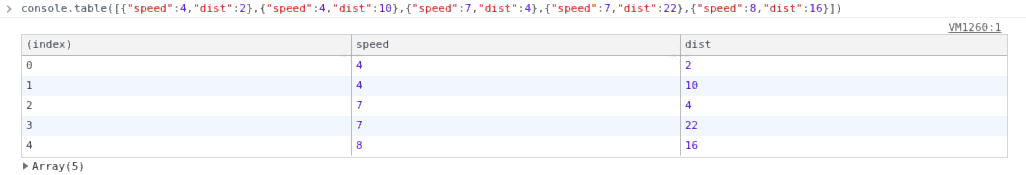
\includegraphics{images/console-table.png}
\caption{console.table output}
\end{figure}

We can reproduce this with the snippet below, we remove row names and use apply to turn every row into a list.

\begin{Shaded}
\begin{Highlighting}[]
\KeywordTok{row.names}\NormalTok{(df) <{-}}\StringTok{ }\OtherTok{NULL}
\NormalTok{df\_list <{-}}\StringTok{ }\KeywordTok{apply}\NormalTok{(df, }\DecValTok{1}\NormalTok{, as.list)}

\KeywordTok{toJSON}\NormalTok{(df\_list, }\DataTypeTok{pretty =} \OtherTok{TRUE}\NormalTok{, }\DataTypeTok{auto\_unbox =} \OtherTok{TRUE}\NormalTok{)}
\end{Highlighting}
\end{Shaded}

\begin{verbatim}
## [
##   {
##     "speed": 4,
##     "dist": 2
##   },
##   {
##     "speed": 4,
##     "dist": 10
##   }
## ]
\end{verbatim}

Jsonlite of course also enables reading data from JSON into R with the function \texttt{fromJSON}.

\begin{Shaded}
\begin{Highlighting}[]
\NormalTok{json <{-}}\StringTok{ }\KeywordTok{toJSON}\NormalTok{(df) }\CommentTok{\# convert to JSON}
\KeywordTok{fromJSON}\NormalTok{(json) }\CommentTok{\# read from JSON}
\end{Highlighting}
\end{Shaded}

\begin{verbatim}
##   speed dist
## 1     4    2
## 2     4   10
\end{verbatim}

It's important to note that jsonlite did the conversion back to a data frame. Therefore the code below also returns a data frame even though the object we initially converted to JSON is a list.

\begin{Shaded}
\begin{Highlighting}[]
\KeywordTok{class}\NormalTok{(df\_list)}
\end{Highlighting}
\end{Shaded}

\begin{verbatim}
## [1] "list"
\end{verbatim}

\begin{Shaded}
\begin{Highlighting}[]
\NormalTok{json <{-}}\StringTok{ }\KeywordTok{toJSON}\NormalTok{(df\_list)}
\KeywordTok{fromJSON}\NormalTok{(json)}
\end{Highlighting}
\end{Shaded}

\begin{verbatim}
##   speed dist
## 1     4    2
## 2     4   10
\end{verbatim}

Jsonlite provides many more options and functions that will let you tune how JSON data is read and written. Also, the jsonlite package does far more than what we detailed in this section but at this juncture this is an adequate understanding of things.

\hypertarget{javascript}{%
\section{JavaScript}\label{javascript}}

The book is not meant to teach one JavaScript, only to show how graciously it can work with R. Let us thus go through the very basics to ensure we know enough to get started with the coming chapters.

The easiest way to run JavaScript interactively is probably to create an HTML file (e.g.: \texttt{try.html}), write your code within a \texttt{\textless{}script\textgreater{}} tags and open the file in your web browser. The console output can be observed in the console of the browser, developer tools (more on that below).

\begin{Shaded}
\begin{Highlighting}[]
\ErrorTok{<}\NormalTok{!–– index.html ––>}
\KeywordTok{<html>}
  \KeywordTok{<head>}
  \KeywordTok{</head>}
  \KeywordTok{<body>}
    \KeywordTok{<p}\OtherTok{ id=}\StringTok{"content"}\KeywordTok{>}\NormalTok{Trying JavaScript!}\KeywordTok{</p>}
  \KeywordTok{</body>}
  \KeywordTok{<script>}
    \CommentTok{// place your JavaScript code here}
    \VariableTok{console}\NormalTok{.}\AttributeTok{log}\NormalTok{(}\StringTok{\textquotesingle{}Hello JavaScript!\textquotesingle{}}\NormalTok{)}
  \KeywordTok{</script>}
\KeywordTok{</html>}
\end{Highlighting}
\end{Shaded}

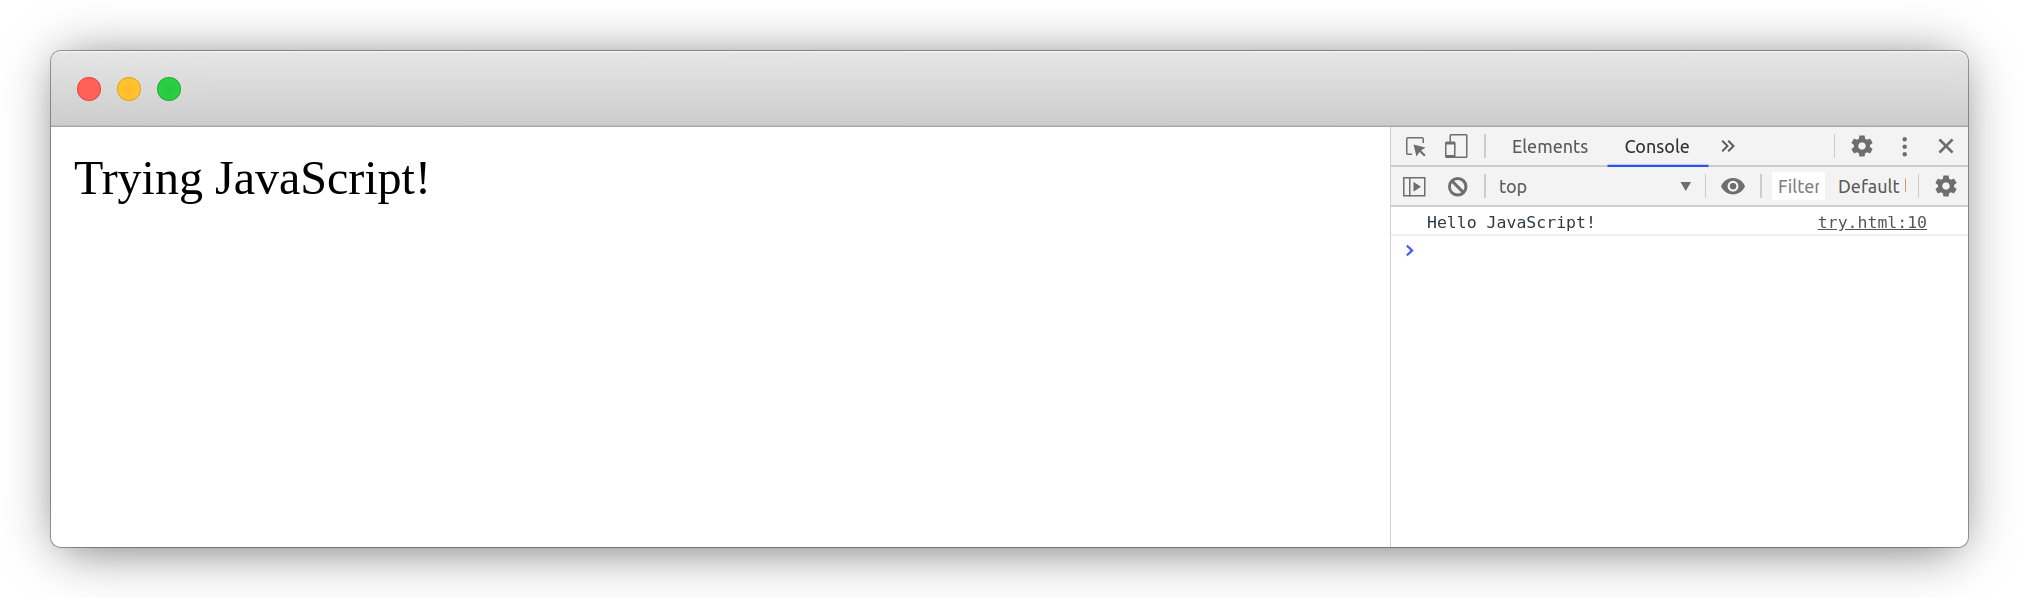
\includegraphics{images/tryingjs.png}

\hypertarget{developer-tools}{%
\subsection{Developer tools}\label{developer-tools}}

Most of the JavaScript code written in this book is intended to be run in web browsers, it is thus vital that you have a great understanding of your web browser and its developer tools (devtools). In this section we discuss those available in Google Chrome and Chromium but such tools, albeit somewhat different, also exist in Mozilla Firefox.

\begin{rmdnote}
The RStudio IDE is built on Chromium, some of these tools will therefore
also work in RStudio.
\end{rmdnote}

The easiest way to access the developer the developer tools from the browser is by ``inspecting:'' right click on an element on a webpage and select ``inspect''. This will open the developer tools either at the bottom or on the right of the page.

\begin{figure}
\centering
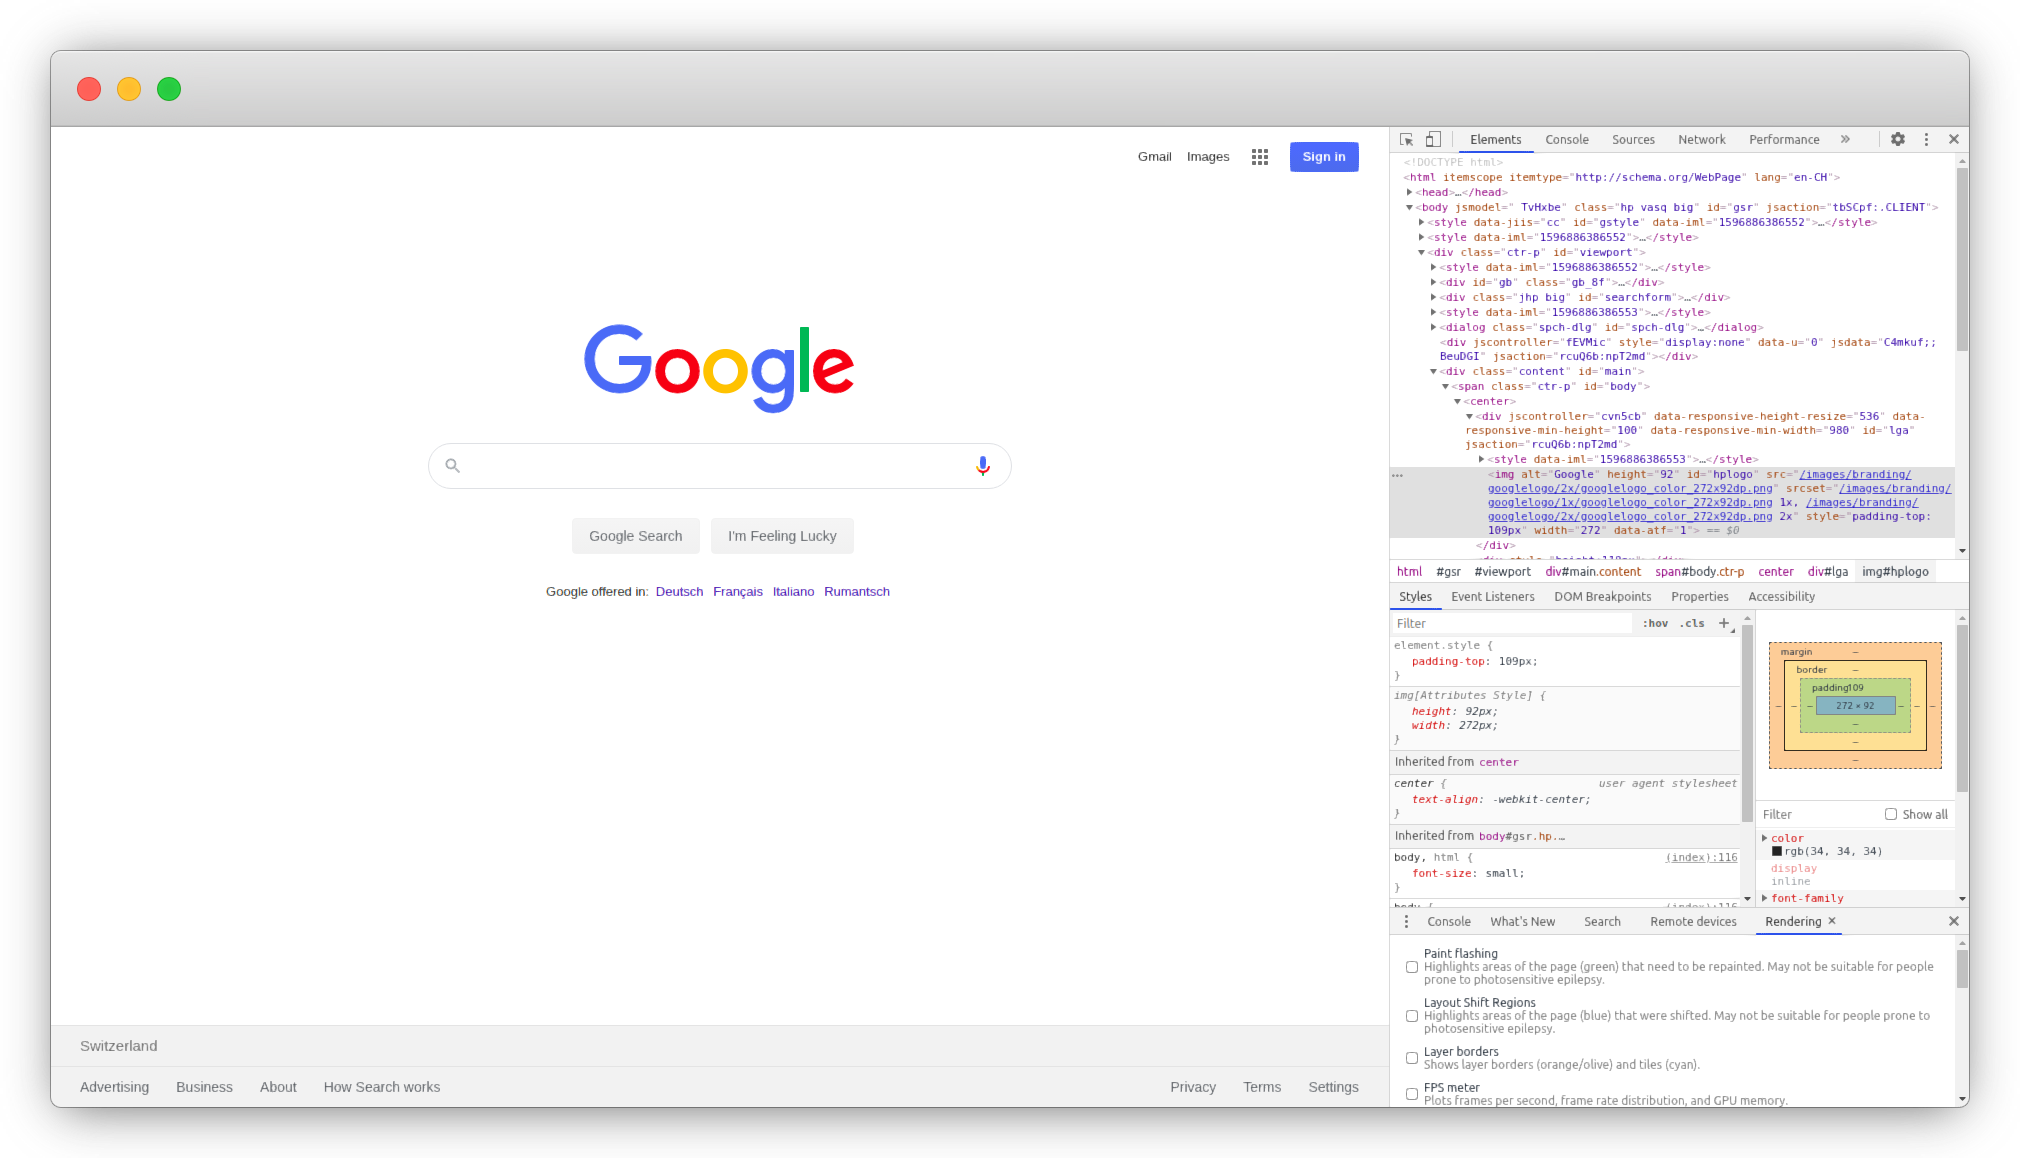
\includegraphics{images/devtools.png}
\caption{Google Chrome Devtools}
\end{figure}

The developer tools pane consists of several tabs but we will mainly use:

\begin{enumerate}
\def\labelenumi{\arabic{enumi}.}
\tightlist
\item
  Elements: Presents the DOM Tree, the HTML document structure, great for inspecting the structure of the outputs generated from R.
\item
  Console: The JavaScript console where messages, errors, and other such things are logged. Essential for debugging.
\end{enumerate}

\hypertarget{variable-declaration-and-scope}{%
\subsection{Variable declaration and scope}\label{variable-declaration-and-scope}}

One major way JavaScript differs from R is that variables must be declared using one of three keywords, \texttt{var}, \texttt{let}, or \texttt{const} which mainly affect the scope where the declared variable will be accessible from.

\begin{Shaded}
\begin{Highlighting}[]
\NormalTok{x }\OperatorTok{=} \DecValTok{1}\OperatorTok{;} \CommentTok{// error}
\KeywordTok{var}\NormalTok{ x }\OperatorTok{=} \DecValTok{1}\OperatorTok{;} \CommentTok{// works}
\end{Highlighting}
\end{Shaded}

One can declare a variable without assigning a value to it, to then do so later on.

\begin{Shaded}
\begin{Highlighting}[]
\KeywordTok{var}\NormalTok{ y}\OperatorTok{;} \CommentTok{// declare }
\NormalTok{y }\OperatorTok{=}\NormalTok{ [}\DecValTok{1}\OperatorTok{,}\DecValTok{2}\OperatorTok{,}\DecValTok{3}\NormalTok{]}\OperatorTok{;} \CommentTok{// define it as array}
\NormalTok{y }\OperatorTok{=} \StringTok{\textquotesingle{}string\textquotesingle{}}\OperatorTok{;} \CommentTok{// change to character string}
\end{Highlighting}
\end{Shaded}

The \texttt{let} and \texttt{const} keywords were added in ES2015, the \texttt{const} is used to defined a constant: a variable that once declared cannot be changed.

\begin{Shaded}
\begin{Highlighting}[]
\KeywordTok{const}\NormalTok{ x }\OperatorTok{=} \DecValTok{1}\OperatorTok{;} \CommentTok{// declare constant}
\NormalTok{x }\OperatorTok{=} \DecValTok{2}\OperatorTok{;} \CommentTok{// error}
\end{Highlighting}
\end{Shaded}

Though this is probably only rarely done in R, one can produce something similar by locking the binding for a variable in its environment.

\begin{Shaded}
\begin{Highlighting}[]
\NormalTok{x <{-}}\StringTok{ }\DecValTok{1} \CommentTok{\# declare x}
\KeywordTok{lockBinding}\NormalTok{(}\StringTok{"x"}\NormalTok{, }\DataTypeTok{env =}\NormalTok{ .GlobalEnv) }\CommentTok{\# make constant}
\NormalTok{x <{-}}\StringTok{ }\DecValTok{2} \CommentTok{\# error}
\end{Highlighting}
\end{Shaded}

\begin{verbatim}
## Error in eval(expr, envir, enclos): cannot change value of locked binding for 'x'
\end{verbatim}

\begin{Shaded}
\begin{Highlighting}[]
\KeywordTok{unlockBinding}\NormalTok{(}\StringTok{"x"}\NormalTok{, }\DataTypeTok{env =}\NormalTok{ .GlobalEnv) }\CommentTok{\# unlock binding}
\NormalTok{x <{-}}\StringTok{ }\DecValTok{2} \CommentTok{\# works}
\end{Highlighting}
\end{Shaded}

The \texttt{let} keyword is akin to declaring a variable with the \texttt{var} keyword, however \texttt{let} (and \texttt{const}) will declare the variable in the ``block scope.'' This in effect further narrows down the scope where the variable will be accessible, a block scope is generally the area within \texttt{if}, \texttt{switch} conditions or \texttt{for} and \texttt{while} loops: areas within curly brackets.

\begin{Shaded}
\begin{Highlighting}[]
\ControlFlowTok{if}\NormalTok{(}\KeywordTok{true}\NormalTok{)}\OperatorTok{\{}
  \KeywordTok{let}\NormalTok{ x }\OperatorTok{=} \DecValTok{1}\OperatorTok{;}
  \KeywordTok{var}\NormalTok{ y }\OperatorTok{=} \DecValTok{1}\OperatorTok{;}
\OperatorTok{\}}

\VariableTok{console}\NormalTok{.}\AttributeTok{log}\NormalTok{(x) }\CommentTok{// error x does not exist}
\VariableTok{console}\NormalTok{.}\AttributeTok{log}\NormalTok{(y) }\CommentTok{// works}
\end{Highlighting}
\end{Shaded}

In the above example \texttt{x} is only accessible within the if statement as it is declared with \texttt{let}, \texttt{var} does not have a block scope.

While on the subject of scope, in R like in JavaScript, variables can be accessed from the parent environment (often referred to as ``context'' in the latter). One immense difference though is that while it is seen as bad practice in R it is not in JavaScript where it is extremely useful.

\begin{Shaded}
\begin{Highlighting}[]
\CommentTok{\# it works but don\textquotesingle{}t do this in R}
\NormalTok{x <{-}}\StringTok{ }\DecValTok{123}
\NormalTok{foo <{-}}\StringTok{ }\ControlFlowTok{function}\NormalTok{()\{}
  \KeywordTok{print}\NormalTok{(x)}
\NormalTok{\}}
\KeywordTok{foo}\NormalTok{()}
\end{Highlighting}
\end{Shaded}

\begin{verbatim}
## [1] 123
\end{verbatim}

The above R code can be re-written in JavaScript. Note the slight variation in the function declaration.

\begin{Shaded}
\begin{Highlighting}[]
\CommentTok{// this is perfectly fine}
\KeywordTok{var}\NormalTok{ x }\OperatorTok{=} \DecValTok{1}\OperatorTok{;}

\KeywordTok{function} \AttributeTok{foo}\NormalTok{()}\OperatorTok{\{}
  \VariableTok{console}\NormalTok{.}\AttributeTok{log}\NormalTok{(x)}\OperatorTok{;} \CommentTok{// print to console}
\OperatorTok{\}}

\AttributeTok{foo}\NormalTok{()}\OperatorTok{;}
\end{Highlighting}
\end{Shaded}

\begin{rmdnote}
Accessing variables from the parent environment (context) is useful in
JavaScript but should not be done in R
\end{rmdnote}

\hypertarget{document-object-model}{%
\subsection{Document object model}\label{document-object-model}}

One concept which does not exist in R is that of the ``DOM'' which stands for Document Object Model. When a web page is loaded, the browser creates a Document Object Model of the web page which can be accessed in JavaScript from the \texttt{document} object. This lets the developer programmatically manipulate the page itself so one can for instance, add an element (e.g.: a button), change the text of another, and plenty more.

The JavaScript code below grabs the element where \texttt{id=\textquotesingle{}content\textquotesingle{}} from the \texttt{document} with \texttt{getElementById} and replaces the text (\texttt{innerText}). Even though the page only contains ``Trying JavaScript!'' when the page is opened (loaded) in the web browser JavaScript runs the code and changes it: this happens very fast so the original text cannot be seen.

\begin{Shaded}
\begin{Highlighting}[]
 \ErrorTok{<}\NormalTok{!–– index.html ––>}
\KeywordTok{<html>}
  \KeywordTok{<head>}
  \KeywordTok{</head>}
  \KeywordTok{<body>}
    \KeywordTok{<p}\OtherTok{ id=}\StringTok{"content"}\KeywordTok{>}\NormalTok{Trying JavaScript!}\KeywordTok{</p>}
  \KeywordTok{</body>}
  \KeywordTok{<script>}
    \KeywordTok{var}\NormalTok{ cnt }\OperatorTok{=} \VariableTok{document}\NormalTok{.}\AttributeTok{getElementById}\NormalTok{(}\StringTok{"content"}\NormalTok{)}\OperatorTok{;}
    \VariableTok{cnt}\NormalTok{.}\AttributeTok{innerText} \OperatorTok{=} \StringTok{"The text has changed"}\OperatorTok{;}
  \KeywordTok{</script>}
\KeywordTok{</html>}
\end{Highlighting}
\end{Shaded}

One final thing to note for future reference, though not limited to the ids or classes most such selection of elements from the DOM are done with those where the pound sign refers to an element's id (\texttt{\#id}) and a dot refers to an element's class (\texttt{.class}), just like in CSS.

\begin{Shaded}
\begin{Highlighting}[]
 \ErrorTok{<}\NormalTok{!–– index.html ––>}
\KeywordTok{<html>}
  \KeywordTok{<head>}
  \KeywordTok{</head>}
  \KeywordTok{<body>}
    \KeywordTok{<p}\OtherTok{ id=}\StringTok{"content"}\OtherTok{ class=}\StringTok{"stuff"}\KeywordTok{>}\NormalTok{Trying JavaScript!}\KeywordTok{</p>}
  \KeywordTok{</body>}
  \KeywordTok{<script>}
    \CommentTok{// select by id}
    \KeywordTok{var}\NormalTok{ x }\OperatorTok{=} \VariableTok{document}\NormalTok{.}\AttributeTok{getElementById}\NormalTok{(}\StringTok{"content"}\NormalTok{)}\OperatorTok{;}
    \KeywordTok{var}\NormalTok{ y }\OperatorTok{=} \VariableTok{document}\NormalTok{.}\AttributeTok{querySelector}\NormalTok{(}\StringTok{"\#content"}\NormalTok{)}\OperatorTok{;}

    \VariableTok{console}\NormalTok{.}\AttributeTok{log}\NormalTok{(x }\OperatorTok{==}\NormalTok{ y)}\OperatorTok{;} \CommentTok{// true}

    \CommentTok{// select by class}
    \KeywordTok{var}\NormalTok{ z }\OperatorTok{=} \VariableTok{document}\NormalTok{.}\AttributeTok{querySelector}\NormalTok{(}\StringTok{".stuff"}\NormalTok{)}\OperatorTok{;}
  \KeywordTok{</script>}
\KeywordTok{</html>}
\end{Highlighting}
\end{Shaded}

Getting elements from the DOM is a very common operation in JavaScript. While a class can be applied to multiple elements which is useful to get and apply actions to multiple elements, the id attribute must be unique (no two elements can bear the same id in the HTML document) is useful to retrieve a specific element.

Interestingly some of that mechanism is used by shiny to retrieve and manipulate inputs, the argument \texttt{inputId} of shiny inputs effectively define the HTML \texttt{id} attribute of said input. Shiny can then internally make use of functions the likes of \texttt{getElementById} in order to get those inputs, set or update their values, etc.

\begin{Shaded}
\begin{Highlighting}[]
\NormalTok{shiny}\OperatorTok{::}\KeywordTok{actionButton}\NormalTok{(}\DataTypeTok{inputId =} \StringTok{"theId"}\NormalTok{, }\DataTypeTok{label =} \StringTok{"the label"}\NormalTok{) }
\end{Highlighting}
\end{Shaded}

the label

This of course only scratches the surface of JavaScript thus this provides ample understanding of the language to keep up with the next chapters. Also, a somewhat interesting fact that will prove useful later in the book: the RStudio IDE is actually a browser, therefore, in the IDE, one can right-click and ``inspect element'' to view the rendered source code.

\hypertarget{part-data-visualisation}{%
\part{Data Visualisation}\label{part-data-visualisation}}

\hypertarget{introduction-to-widgets}{%
\chapter{Introduction to widgets}\label{introduction-to-widgets}}

This part of the book explores the integration of JavaScript with R using the htmlwidgets package which focuses on libraries that produce a visual output, it is often used for data visualisation but is not limited to it.

As in previous parts of this book we mainly learn through examples, building multiple widgets of increasing complexity as we progress through the chapter. Before writing the first widget, we explore existing R packages that allow creating interactive data visualisations this give a first glimpse at we build in this part of the book. Then we explore JavaScript libraries that make great candidates for htmlwidgets and attempt to understand how they work to grasp what is expected from the developer in order to integrate them with R. Finally, we build up on the previous chapter to improve how htmlwidgets work with shiny.

\hypertarget{plotly-package}{%
\section{Plotly package}\label{plotly-package}}

\hypertarget{dt-package}{%
\section{DT package}\label{dt-package}}

\hypertarget{basics-of-building-widgets}{%
\chapter{Basics of building widgets}\label{basics-of-building-widgets}}

Having explored existing packages that build on top of the htmlwidgets package gives some idea of the end product we learn to build but it does not give insights about where to start and much of how it works probably remains somewhat magical.

\hypertarget{candidate-libraries}{%
\section{Candidate Libraries}\label{candidate-libraries}}

Before going down the rabbit hole it is good to take a look at the types of libraries one will work with. As htmlwidgets' main clients are JavaScript visualisation libraries let us take a look at some such popular libraries and briefly analyse at how they work and what they have in common. This will greatly help conceptualise what one is trying to achieve in this chapter.

\hypertarget{plotly}{%
\subsection{Plotly}\label{plotly}}

\href{https://plotly.com/javascript/}{Plotly.js} is probably one of the more popular out there, it provides over 40 fully customiseable chart types, many of which are very sophisticated. This is indeed the JavaScript library used by the R package of the same name: plotly.

Looking at the code presented in the ``Get Started'' guide reveals just how convenient the library is. One must import plotly, of course, then have a \texttt{\textless{}div\textgreater{}} where the visualisation will be placed, then, using \texttt{Plotly.newPlot}, create the actual visualisation by passing it first the element previously mentioned and a JSON of options that describe the chart.

\begin{Shaded}
\begin{Highlighting}[]
\DataTypeTok{<!DOCTYPE }\NormalTok{html}\DataTypeTok{>}
\KeywordTok{<html}\OtherTok{ xmlns=}\StringTok{"http://www.w3.org/1999/xhtml"}\OtherTok{ lang=}\StringTok{""}\OtherTok{ xml:lang=}\StringTok{""}\KeywordTok{>}

\KeywordTok{<head>}
  \CommentTok{<!{-}{-} Import library {-}{-}>}
  \KeywordTok{<script}\OtherTok{ src=}\StringTok{"plotly{-}latest.min.js"}\KeywordTok{></script>}
\KeywordTok{</head>}

\KeywordTok{<body>}
  \CommentTok{<!{-}{-} div to hold visualisation {-}{-}>}
  \KeywordTok{<div}\OtherTok{ id=}\StringTok{"chart"}\OtherTok{ style=}\StringTok{"width:600px;height:400px;"}\KeywordTok{></div>}

  \CommentTok{<!{-}{-} Script to create visualisation {-}{-}>}
  \KeywordTok{<script>}
\NormalTok{    el }\OperatorTok{=} \VariableTok{document}\NormalTok{.}\AttributeTok{getElementById}\NormalTok{(}\StringTok{\textquotesingle{}chart\textquotesingle{}}\NormalTok{)}\OperatorTok{;}
    \VariableTok{Plotly}\NormalTok{.}\AttributeTok{newPlot}\NormalTok{(el}\OperatorTok{,}\NormalTok{ [}\OperatorTok{\{}
      \DataTypeTok{x}\OperatorTok{:}\NormalTok{ [}\DecValTok{1}\OperatorTok{,} \DecValTok{2}\OperatorTok{,} \DecValTok{3}\OperatorTok{,} \DecValTok{4}\OperatorTok{,} \DecValTok{5}\NormalTok{]}\OperatorTok{,}
      \DataTypeTok{y}\OperatorTok{:}\NormalTok{ [}\DecValTok{1}\OperatorTok{,} \DecValTok{2}\OperatorTok{,} \DecValTok{4}\OperatorTok{,} \DecValTok{8}\OperatorTok{,} \DecValTok{16}\NormalTok{] }\OperatorTok{\}}\NormalTok{]}
\NormalTok{    )}\OperatorTok{;}
  \KeywordTok{</script>}
\KeywordTok{</body>}

\KeywordTok{</html>}
\end{Highlighting}
\end{Shaded}

\begin{figure}
\centering
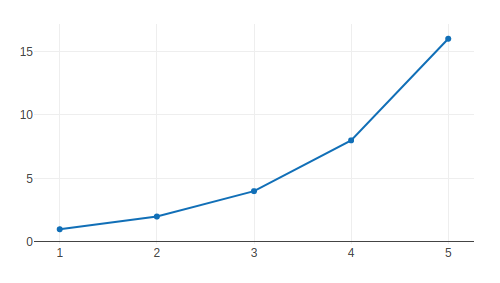
\includegraphics{images/candidate-plotly.png}
\caption{Plotly.js example}
\end{figure}

Now let's look at how another popular library does it.

\hypertarget{highchart.js}{%
\subsection{Highchart.js}\label{highchart.js}}

\href{https://www.highcharts.com/}{Highcharts} is another library which allows creating gorgeous visualisation, maps, and more, it's also very popular albeit not being entirely open-source.

\begin{Shaded}
\begin{Highlighting}[]
\DataTypeTok{<!DOCTYPE }\NormalTok{html}\DataTypeTok{>}
\KeywordTok{<html}\OtherTok{ xmlns=}\StringTok{"http://www.w3.org/1999/xhtml"}\OtherTok{ lang=}\StringTok{""}\OtherTok{ xml:lang=}\StringTok{""}\KeywordTok{>}

\KeywordTok{<head>}
  \CommentTok{<!{-}{-} Import library {-}{-}>}
  \KeywordTok{<script}\OtherTok{ src=}\StringTok{"highcharts.js"}\KeywordTok{></script>}
\KeywordTok{</head>}

\KeywordTok{<body>}
  \CommentTok{<!{-}{-} div to hold visualisation {-}{-}>}
  \KeywordTok{<div}\OtherTok{ id=}\StringTok{"chart"}\OtherTok{ style=}\StringTok{"width:100\%;height:400px;"}\KeywordTok{></div>}

  \CommentTok{<!{-}{-} Script to create visualisation {-}{-}>}
  \KeywordTok{<script>}
    \KeywordTok{var}\NormalTok{ myChart }\OperatorTok{=} \VariableTok{Highcharts}\NormalTok{.}\AttributeTok{chart}\NormalTok{(}\StringTok{\textquotesingle{}chart\textquotesingle{}}\OperatorTok{,} \OperatorTok{\{}
        \DataTypeTok{xAxis}\OperatorTok{:} \OperatorTok{\{}
            \DataTypeTok{categories}\OperatorTok{:}\NormalTok{ [}\StringTok{\textquotesingle{}Apples\textquotesingle{}}\OperatorTok{,} \StringTok{\textquotesingle{}Bananas\textquotesingle{}}\OperatorTok{,} \StringTok{\textquotesingle{}Oranges\textquotesingle{}}\NormalTok{]}
        \OperatorTok{\},}
        \DataTypeTok{series}\OperatorTok{:}\NormalTok{ [}\OperatorTok{\{}
            \DataTypeTok{name}\OperatorTok{:} \StringTok{\textquotesingle{}Jane\textquotesingle{}}\OperatorTok{,}
            \DataTypeTok{data}\OperatorTok{:}\NormalTok{ [}\DecValTok{1}\OperatorTok{,} \DecValTok{0}\OperatorTok{,} \DecValTok{4}\NormalTok{]}
        \OperatorTok{\},} \OperatorTok{\{}
            \DataTypeTok{name}\OperatorTok{:} \StringTok{\textquotesingle{}John\textquotesingle{}}\OperatorTok{,}
            \DataTypeTok{data}\OperatorTok{:}\NormalTok{ [}\DecValTok{5}\OperatorTok{,} \DecValTok{7}\OperatorTok{,} \DecValTok{3}\NormalTok{]}
        \OperatorTok{\}}\NormalTok{]}
    \OperatorTok{\}}\NormalTok{)}\OperatorTok{;}
  \KeywordTok{</script>}
\KeywordTok{</body>}

\KeywordTok{</html>}
\end{Highlighting}
\end{Shaded}

\begin{figure}
\centering
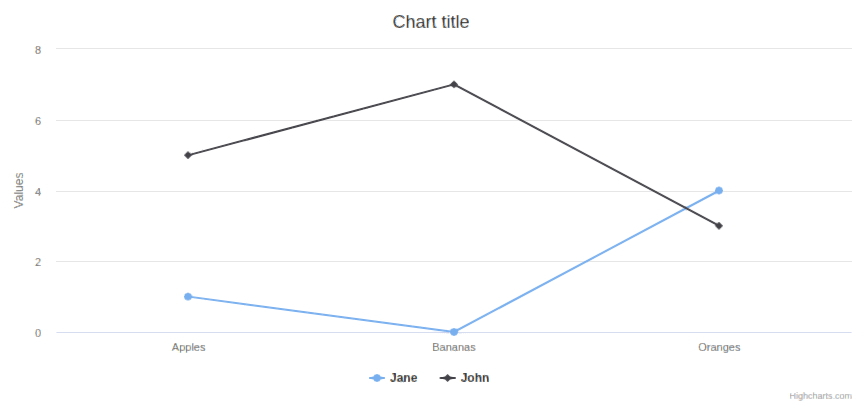
\includegraphics{images/candidate-highcharts.png}
\caption{Highcharts example}
\end{figure}

The above is very similar to what plotly.js requires: import libraries, create a \texttt{\textless{}div\textgreater{}} where to put the visualisation, and, to create the chart, run a function which also takes the id of the div where to place the chart and a JSON of options defining the actual chart, including the data.

\hypertarget{chart.js}{%
\subsection{Chart.js}\label{chart.js}}

\href{https://www.chartjs.org/}{Chart.js} is yet another library which to draw standard charts popular for its permissive license and convenient API.

\begin{Shaded}
\begin{Highlighting}[]
\DataTypeTok{<!DOCTYPE }\NormalTok{html}\DataTypeTok{>}
\KeywordTok{<html}\OtherTok{ xmlns=}\StringTok{"http://www.w3.org/1999/xhtml"}\OtherTok{ lang=}\StringTok{""}\OtherTok{ xml:lang=}\StringTok{""}\KeywordTok{>}

\KeywordTok{<head>}
  \CommentTok{<!{-}{-} Import library {-}{-}>}
  \KeywordTok{<script}\OtherTok{ src=}\StringTok{"Chart.min.js"}\KeywordTok{></script>}
\KeywordTok{</head>}

\KeywordTok{<body>}
  \CommentTok{<!{-}{-} canvas to hold visualisation {-}{-}>}
  \KeywordTok{<canvas}\OtherTok{ id=}\StringTok{"chart"}\KeywordTok{></canvas>}

  \CommentTok{<!{-}{-} Script to create visualisation {-}{-}>}
  \KeywordTok{<script>}
    \KeywordTok{var}\NormalTok{ el }\OperatorTok{=} \VariableTok{document}\NormalTok{.}\AttributeTok{getElementById}\NormalTok{(}\StringTok{\textquotesingle{}chart\textquotesingle{}}\NormalTok{).}\AttributeTok{getContext}\NormalTok{(}\StringTok{\textquotesingle{}2d\textquotesingle{}}\NormalTok{)}\OperatorTok{;}    
    \KeywordTok{var}\NormalTok{ myChart }\OperatorTok{=} \KeywordTok{new} \AttributeTok{Chart}\NormalTok{(el}\OperatorTok{,} \OperatorTok{\{}
      \DataTypeTok{type}\OperatorTok{:} \StringTok{\textquotesingle{}bar\textquotesingle{}}\OperatorTok{,}
      \DataTypeTok{data}\OperatorTok{:} \OperatorTok{\{}
        \DataTypeTok{labels}\OperatorTok{:}\NormalTok{ [}\StringTok{\textquotesingle{}Red\textquotesingle{}}\OperatorTok{,} \StringTok{\textquotesingle{}Blue\textquotesingle{}}\OperatorTok{,} \StringTok{\textquotesingle{}Yellow\textquotesingle{}}\OperatorTok{,} \StringTok{\textquotesingle{}Green\textquotesingle{}}\OperatorTok{,} \StringTok{\textquotesingle{}Purple\textquotesingle{}}\OperatorTok{,} \StringTok{\textquotesingle{}Orange\textquotesingle{}}\NormalTok{]}\OperatorTok{,}
        \DataTypeTok{datasets}\OperatorTok{:}\NormalTok{ [}\OperatorTok{\{}
          \DataTypeTok{label}\OperatorTok{:} \StringTok{\textquotesingle{}\# of Votes\textquotesingle{}}\OperatorTok{,}
          \DataTypeTok{data}\OperatorTok{:}\NormalTok{ [}\DecValTok{12}\OperatorTok{,} \DecValTok{19}\OperatorTok{,} \DecValTok{3}\OperatorTok{,} \DecValTok{5}\OperatorTok{,} \DecValTok{2}\OperatorTok{,} \DecValTok{3}\NormalTok{]}
        \OperatorTok{\}}\NormalTok{]}
      \OperatorTok{\}}
    \OperatorTok{\}}\NormalTok{)}\OperatorTok{;}
  \KeywordTok{</script>}
\KeywordTok{</body>}

\KeywordTok{</html>}
\end{Highlighting}
\end{Shaded}

\begin{figure}
\centering
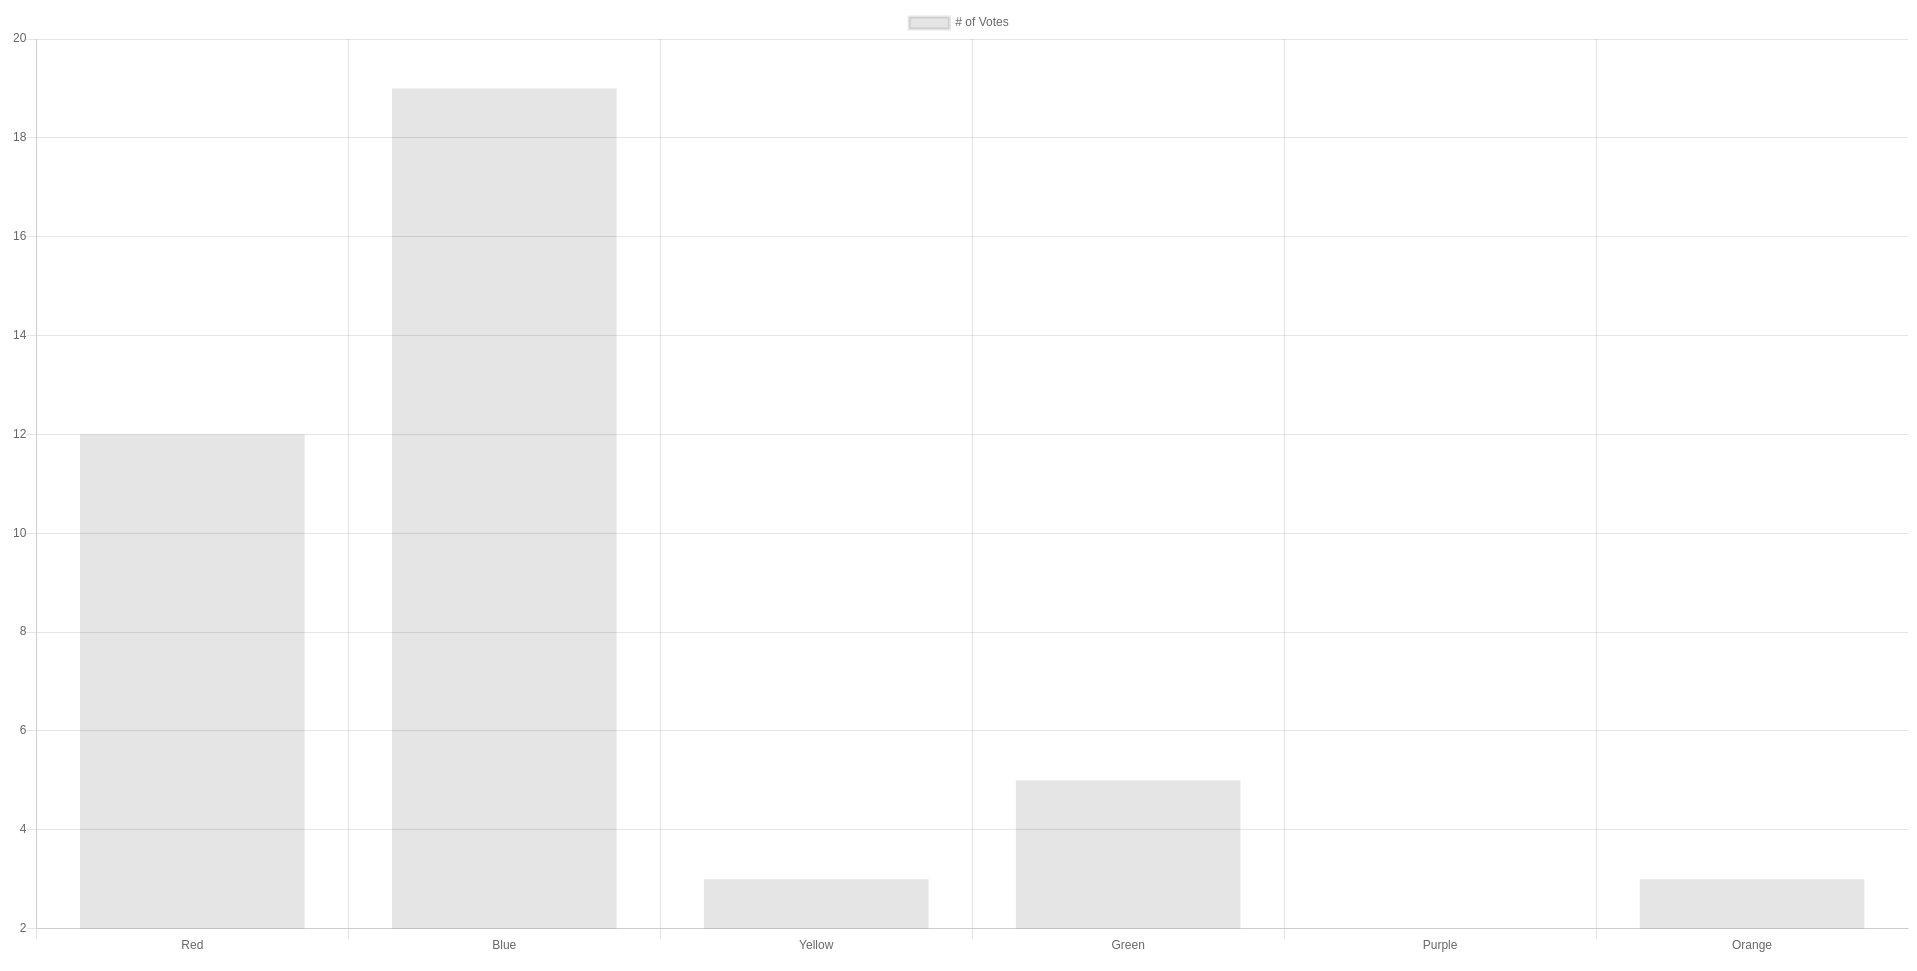
\includegraphics{images/candidate-chartjs.png}
\caption{Chart.js example}
\end{figure}

We again observe a very similar structure as with previous libraries. The library is imported, instead of a \texttt{div} chart.js uses a \texttt{canvas}, and the visualisation is also created from a single function which takes the canvas as first argument and a JSON of options as second.

Hopefully this reveals the repeating structure such libraries tend to follow as well as demonstrate how little JavaScript code is actually involved. It also hints at what should be reproduced, to some extent at least, using R.

\hypertarget{how-it-works}{%
\section{How it works}\label{how-it-works}}

Imagine there is no such package as htmlwidgets to help create interactive visualisations from R: how would one attempt to go about it?

As observed, an interactive visualisation using JavaScript will be contained within an HTML document, therefore it would probably have to be created first. Secondly, the visualisation that is yet to be created likely relies on external libraries, these would need to be imported in the document. The document should also include an HTML element (e.g.: \texttt{\textless{}div\textgreater{}}) to host said visualisation. Then data would have to be serialised in R and embedded into the document where it should be read by JavaScript code that uses it to create the visualisation. Finally all should be managed to work seamlessly across R markdown, shiny, and other environments.

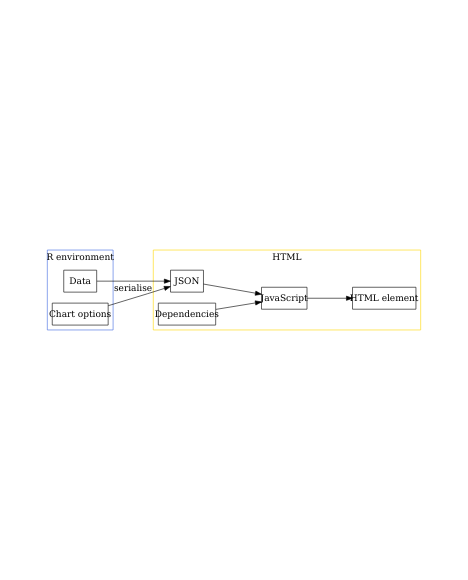
\includegraphics{bookdown_files/figure-latex/unnamed-chunk-22-1.png}

Thankfully the htmlwidgets package is there to handle most of this. Nonetheless, it is important to understand that these operations are undertaken (to some degree) by htmlwidgets.

\hypertarget{your-first-widget}{%
\chapter{Your First Widget}\label{your-first-widget}}

The previous chapter gave some indication as to how widgets work but this is overall probably still shrouded in mystery. This chapter aims at demystifying what remains confusing. This is done by building a very basic widget with the aim of rummaging through its components to observe how they interact and ultimately grasp a greater understanding of how such interactive outputs are actually produced.

\hypertarget{the-scaffold}{%
\section{The Scaffold}\label{the-scaffold}}

Though one could probably create widgets outside of an R package, it would only make things more complicated, htmlwidgets naturally take the form of R packages and are stunningly simple to create. Below we create a package named ``playground'' which will be used to mess around and explore.

\begin{Shaded}
\begin{Highlighting}[]
\KeywordTok{create\_package}\NormalTok{(}\StringTok{"playground"}\NormalTok{)}
\end{Highlighting}
\end{Shaded}

Then, from the root of the package created, we scaffold a widget which we call ``play''.

\begin{Shaded}
\begin{Highlighting}[]
\NormalTok{htmlwidgets}\OperatorTok{::}\KeywordTok{scaffoldWidget}\NormalTok{(}\StringTok{"play"}\NormalTok{)}
\end{Highlighting}
\end{Shaded}

This function puts together the minimalistic structure necessary to implement an HTML widget and opens \texttt{play.R}, \texttt{play.js} and \texttt{play.yaml} in the RStudio IDE or the default text editor.

\begin{rmdnote}
You can scaffold multiple widgets in a single package.
\end{rmdnote}

These files are named after the widget and will form the core of the package. The R file contains core functions of the R API, namely the \texttt{play} function which creates the widget itself, and the \texttt{render*} and \texttt{*output} functions that handle the widget in the shiny server and UI respectively. The \texttt{.js} file contains JavaScript functions that actually generate the visual output.

\begin{Shaded}
\begin{Highlighting}[]
\NormalTok{devtools}\OperatorTok{::}\KeywordTok{document}\NormalTok{()}
\NormalTok{devtools}\OperatorTok{::}\KeywordTok{load\_all}\NormalTok{()}
\end{Highlighting}
\end{Shaded}

It might be hard to believe, but at this stage one already has a fully functioning widget ready to use after documenting, and building the package. Indeed, the \texttt{play.R} file that was created contains a function named ``play'' ẁhich takes, amongst other arguments, a message.

\begin{Shaded}
\begin{Highlighting}[]
\KeywordTok{play}\NormalTok{(}\DataTypeTok{message =} \StringTok{"This is a widget!"}\NormalTok{)}
\end{Highlighting}
\end{Shaded}

\begin{figure}
\centering
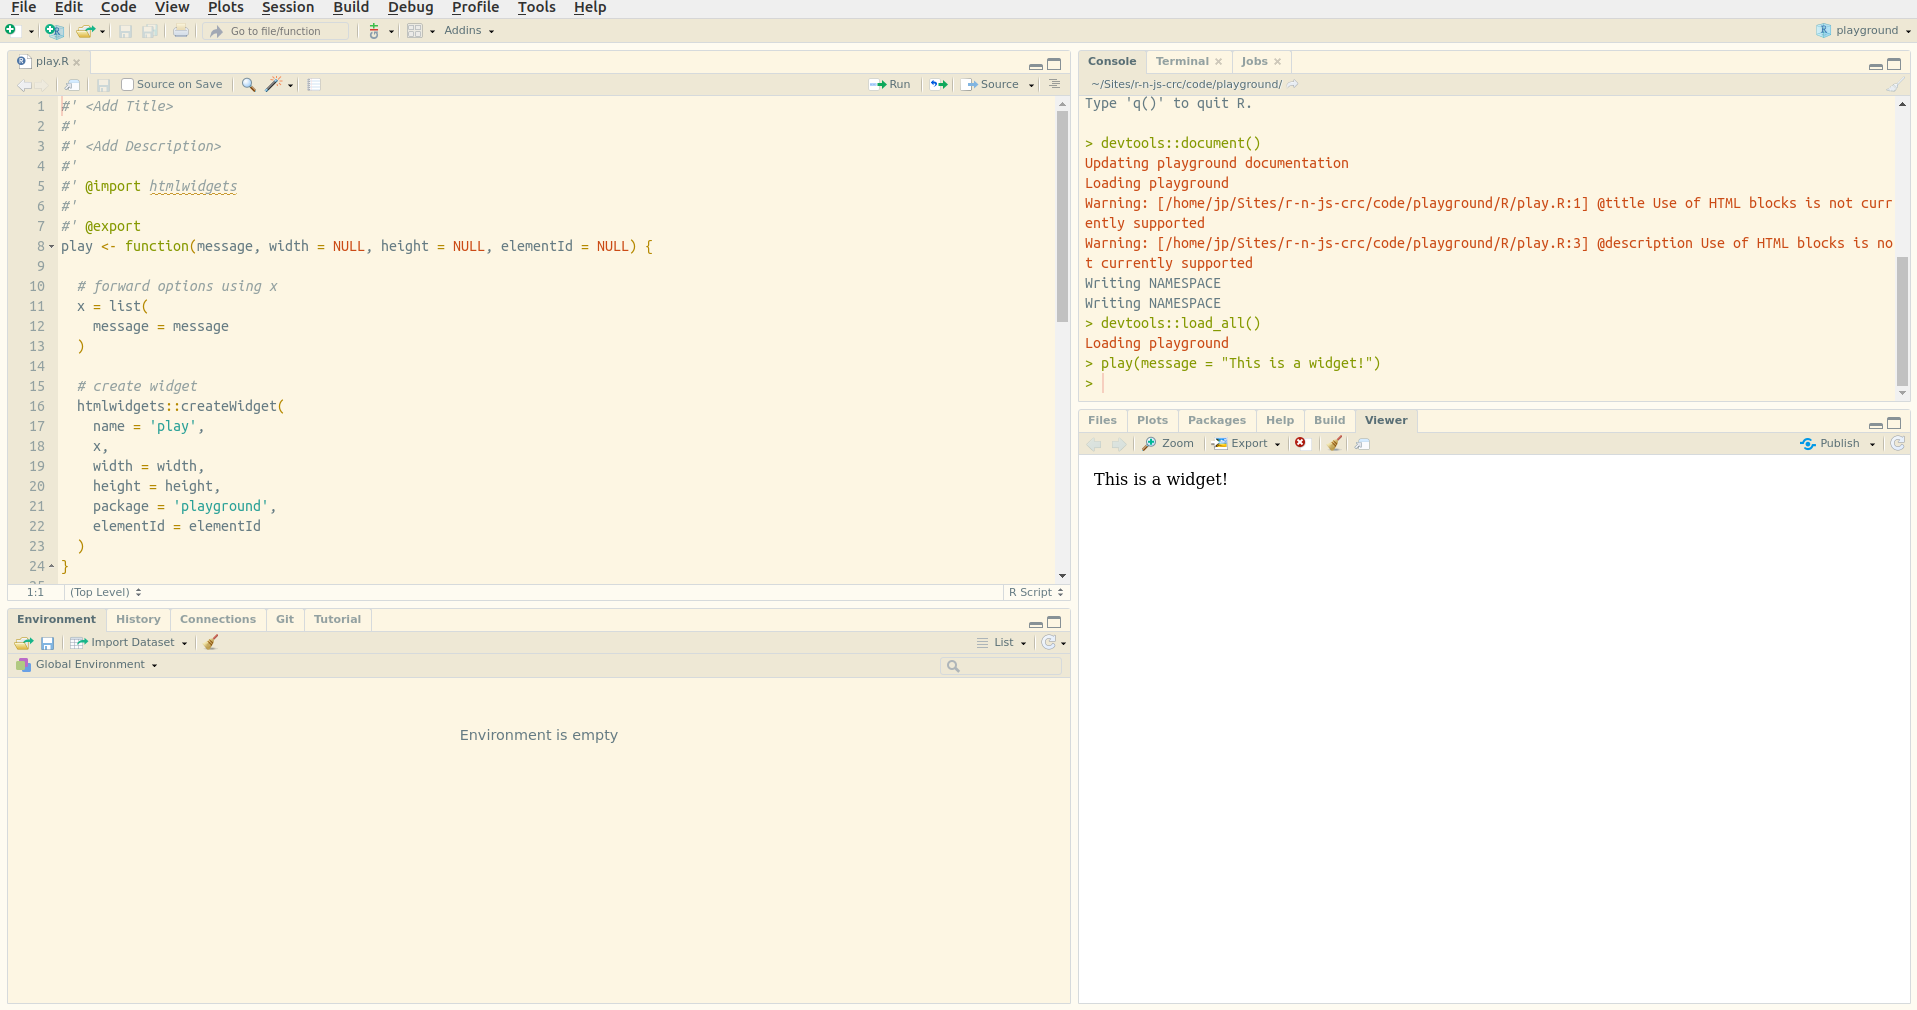
\includegraphics{images/playground-1.png}
\caption{First HTML widget}
\end{figure}

This displays the message in the RStudio ``Viewer,'' or the your default browser which indicates that the function does indeed create an HTML output. One can use the 
\includegraphics{images/open-in-browser.png} button located in the top right of the RStudio ``Viewer'' to open the message in web browser which can prove very useful to look under the hood of the widgets for debugging.

\hypertarget{the-output}{%
\section{The Output}\label{the-output}}

With an out-of-the-box HTML widget package one can start exploring the internals to understand how it works. Let's start by retracing the path taken by the message written in R to its seemingly magical appearance in HTML. The \texttt{play} function previously used, takes the \texttt{message} wraps it into a list which is then used in \texttt{htmlwidgets::createWidget}.

\begin{Shaded}
\begin{Highlighting}[]
\CommentTok{\# forward options using x}
\NormalTok{x =}\StringTok{ }\KeywordTok{list}\NormalTok{(}
  \DataTypeTok{message =}\NormalTok{ message}
\NormalTok{)}
\end{Highlighting}
\end{Shaded}

Wrapping a string in a list might seem unnecessary but one will eventually add variables when building a more complex widget, starting with a list makes it easier to add them later on.

To investigate the widget we should look under the hood; the source code of the created (and rendered) output can be accessed in different ways, 1) by right-clicking on the message displayed in the RStudio Viewer and selecting ``Inspect element,'' or 2) by opening the visualisation in your browser using the 
\includegraphics{images/open-in-browser.png} button located in the top right of the ``Viewer,'' and in the browser right clicking on the message to select ``Inspect.'' The latter is advised as web browsers such as Chrome or Firefox provide much friendlier interfaces for such functionalities as well as shortcuts to inspect or view the source code of a page.

Below is a part of the \texttt{\textless{}body\textgreater{}} of the output of \texttt{play("This\ is\ a\ widget!")} obtained with the method described in the previous paragraph.

\begin{Shaded}
\begin{Highlighting}[]
\KeywordTok{<div}\OtherTok{ id=}\StringTok{"htmlwidget\_container"}\KeywordTok{>}
  \KeywordTok{<div} 
\OtherTok{    id=}\StringTok{"htmlwidget{-}c21cca0e76e520b46fc7"} 
\OtherTok{    style=}\StringTok{"width:960px;height:500px;"} 
\OtherTok{    class=}\StringTok{"play html{-}widget"}\KeywordTok{>}
\NormalTok{    This is a widget!}
  \KeywordTok{</div>}
\KeywordTok{</div>}
\KeywordTok{<script} 
\OtherTok{  type=}\StringTok{"application/json"} 
\OtherTok{  data{-}for=}\StringTok{"htmlwidget{-}c21cca0e76e520b46fc7"}\KeywordTok{>}
  \OperatorTok{\{}\StringTok{"x"}\OperatorTok{:\{}\StringTok{"message"}\OperatorTok{:}\StringTok{"This is a widget!"}\OperatorTok{\},}\StringTok{"evals"}\OperatorTok{:}\NormalTok{[]}\OperatorTok{,}\StringTok{"jsHooks"}\OperatorTok{:}\NormalTok{[]}\OperatorTok{\}}
\KeywordTok{</script>}
\end{Highlighting}
\end{Shaded}

One thing the source code of the rendered output reveals is the element (\texttt{\textless{}div\textgreater{}}) created by the htmlwidgets package to hold the message (the class name is identical to that of the widget, \texttt{play}), as well as, below it, in the \texttt{\textless{}script\textgreater{}} tag, the JSON object which includes the \texttt{x} variable used in the \texttt{play} function. The \texttt{div} created bears a randomly generated \texttt{id} which one can define when creating the widget using the \texttt{elementId} argument.

\begin{Shaded}
\begin{Highlighting}[]
\CommentTok{\# specify the id}
\KeywordTok{play}\NormalTok{(}\StringTok{"This is another widget"}\NormalTok{, }\DataTypeTok{elementId =} \StringTok{"myViz"}\NormalTok{)}
\end{Highlighting}
\end{Shaded}

\begin{Shaded}
\begin{Highlighting}[]
\CommentTok{<!{-}{-} div bears id specified in R {-}{-}>}
\KeywordTok{<div}\OtherTok{ id=}\StringTok{"myViz"} 
\OtherTok{  style=}\StringTok{"width:960px;height:500px;"} 
\OtherTok{  class=}\StringTok{"play html{-}widget"}\KeywordTok{>}
\NormalTok{  This is another widget}
\KeywordTok{</div>}
\end{Highlighting}
\end{Shaded}

You will also notice that this affects the \texttt{script} tag below it, the \texttt{data-for} attribute of which is also set to ``myViz,'' this indicates that it is used to tie the JSON data to a \texttt{div}, essential for htmlwidgets to manage multiple visualisation in R markdown or Shiny for instance. Then again, this happens in the background without the developer (you) having to worry about it.

\begin{Shaded}
\begin{Highlighting}[]
\KeywordTok{<script}\OtherTok{ type=}\StringTok{"application/json"} 
\OtherTok{  data{-}for=}\StringTok{"myViz"}\KeywordTok{>}
  \OperatorTok{\{}\StringTok{"x"}\OperatorTok{:\{}\StringTok{"message"}\OperatorTok{:}\StringTok{"This is a widget!"}\OperatorTok{\},}\StringTok{"evals"}\OperatorTok{:}\NormalTok{[]}\OperatorTok{,}\StringTok{"jsHooks"}\OperatorTok{:}\NormalTok{[]}\OperatorTok{\}}
\KeywordTok{</script>}
\end{Highlighting}
\end{Shaded}

Inspecting the output also shows the dependencies imported, these are placed within the \texttt{head} HTML tags at the top of the page.

\begin{Shaded}
\begin{Highlighting}[]
\KeywordTok{<script}\OtherTok{ src=}\StringTok{"lib/htmlwidgets{-}1.5.1/htmlwidgets.js"}\KeywordTok{></script>}
\KeywordTok{<script}\OtherTok{ src=}\StringTok{"lib/play{-}binding{-}0.0.0.9000/play.js"}\KeywordTok{></script>}
\end{Highlighting}
\end{Shaded}

This effectively imports the \texttt{htmlwidgets.js} library as well as the \texttt{play.js} file, and were the visualisation depending on external libraries they would appear alongside those.

\hypertarget{javascript-side}{%
\section{JavaScript-side}\label{javascript-side}}

Peaking inside the \texttt{play.js} file located at \texttt{inst/htmlwidgets/play.js} reveals the code below:

\begin{Shaded}
\begin{Highlighting}[]
\CommentTok{// play.js}
\VariableTok{HTMLWidgets}\NormalTok{.}\AttributeTok{widget}\NormalTok{(}\OperatorTok{\{}

  \DataTypeTok{name}\OperatorTok{:} \StringTok{\textquotesingle{}play\textquotesingle{}}\OperatorTok{,}

  \DataTypeTok{type}\OperatorTok{:} \StringTok{\textquotesingle{}output\textquotesingle{}}\OperatorTok{,}

  \DataTypeTok{factory}\OperatorTok{:} \KeywordTok{function}\NormalTok{(el}\OperatorTok{,}\NormalTok{ width}\OperatorTok{,}\NormalTok{ height) }\OperatorTok{\{}

    \CommentTok{// }\AlertTok{TODO}\CommentTok{: define shared variables for this instance}

    \ControlFlowTok{return} \OperatorTok{\{}

      \DataTypeTok{renderValue}\OperatorTok{:} \KeywordTok{function}\NormalTok{(x) }\OperatorTok{\{}

        \CommentTok{// }\AlertTok{TODO}\CommentTok{: code to render the widget, e.g.}
        \VariableTok{el}\NormalTok{.}\AttributeTok{innerText} \OperatorTok{=} \VariableTok{x}\NormalTok{.}\AttributeTok{message}\OperatorTok{;}

      \OperatorTok{\},}

      \DataTypeTok{resize}\OperatorTok{:} \KeywordTok{function}\NormalTok{(width}\OperatorTok{,}\NormalTok{ height) }\OperatorTok{\{}

        \CommentTok{// }\AlertTok{TODO}\CommentTok{: code to re{-}render the widget with a new size}

      \OperatorTok{\}}

    \OperatorTok{\};}
  \OperatorTok{\}}
\OperatorTok{\}}\NormalTok{)}\OperatorTok{;}
\end{Highlighting}
\end{Shaded}

However convoluted this may appear at first do not let that intimate you. The name of the widget (\texttt{play}) corresponds to the name used when generating the scaffold, it can also be seen in the \texttt{createWidget} function used inside the \texttt{play.R} file.

\begin{Shaded}
\begin{Highlighting}[]
\NormalTok{htmlwidgets}\OperatorTok{::}\KeywordTok{createWidget}\NormalTok{(}
  \DataTypeTok{name =} \StringTok{\textquotesingle{}play\textquotesingle{}}\NormalTok{,}
\NormalTok{  x,}
  \DataTypeTok{width =}\NormalTok{ width,}
  \DataTypeTok{height =}\NormalTok{ height,}
  \DataTypeTok{package =} \StringTok{\textquotesingle{}playground\textquotesingle{}}\NormalTok{,}
  \DataTypeTok{elementId =}\NormalTok{ elementId}
\NormalTok{)}
\end{Highlighting}
\end{Shaded}

This is so htmlwidgets can internally match the output of \texttt{createWidget} to its JavaScript function.

The \texttt{factory} function returns two functions, \texttt{resize}, and \texttt{renderValue}. The first is used to dynamically resize the output, it is not relevant to this widget is thus tackled later on. Let us focus on \texttt{renderValue}, the function that actually renders the output. It takes an object \texttt{x} from which the ``message'' variable is used as text for object \texttt{el} (\texttt{el.innerText}). The object \texttt{x} passed to this function is actually the list of the same name that was build in the R function \texttt{play}! While in R one would access the \texttt{message} in list \texttt{x} with \texttt{x\$message} in JavaScript to access the \texttt{message} in the JSON \texttt{x} one writes \texttt{x.message}, only changing the dollar sign to a dot. Let's show this perhaps more clearly by printing the content of \texttt{x}.

\begin{Shaded}
\begin{Highlighting}[]
\VariableTok{console}\NormalTok{.}\AttributeTok{log}\NormalTok{(x)}\OperatorTok{;}
\VariableTok{el}\NormalTok{.}\AttributeTok{innerText} \OperatorTok{=} \VariableTok{x}\NormalTok{.}\AttributeTok{message}\OperatorTok{;}
\end{Highlighting}
\end{Shaded}

We place \texttt{console.log} to print the content of \texttt{x} in the console, reload the package with \texttt{devtools::load\_all} and use the function \texttt{play} again then explore the console from the browser (inspect and go to the ``console'' tab).

\begin{figure}
\centering
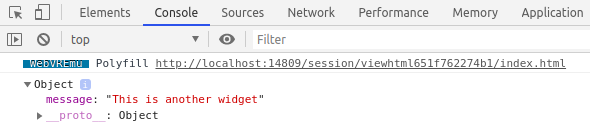
\includegraphics{images/playground-console-x.png}
\caption{Console tab output}
\end{figure}

This displays the JSON object containing the message: it looks eerily similar to the list that was created in R (\texttt{x\ =\ list(message\ =\ "This\ is\ a\ widget!")}). What one should take away from this is that data that needs to be communicated from R to the JavaScript function should be placed in the R list \texttt{x}. This list is serialised to JSON and placed in the HTML output in a \texttt{script} tag with a \texttt{data-for} attribute that indicates which widget the data is destined for. This effectively enables htmlwidgets to match the serialised data with the output elements: data in \texttt{\textless{}script\ data-for=\textquotesingle{}viz\textquotesingle{}\textgreater{}} is to be used to create a visualisation in \texttt{\textless{}div\ id=\textquotesingle{}viz\textquotesingle{}\textgreater{}}.

Before we move on to other things one should also grasp a better understanding of the \texttt{el} object, which can also be logged in the console.

\begin{Shaded}
\begin{Highlighting}[]
\VariableTok{console}\NormalTok{.}\AttributeTok{log}\NormalTok{(x)}\OperatorTok{;}
\VariableTok{console}\NormalTok{.}\AttributeTok{log}\NormalTok{(el)}\OperatorTok{;}
\VariableTok{el}\NormalTok{.}\AttributeTok{innerText} \OperatorTok{=} \VariableTok{x}\NormalTok{.}\AttributeTok{message}\OperatorTok{;}
\end{Highlighting}
\end{Shaded}

\begin{figure}
\centering
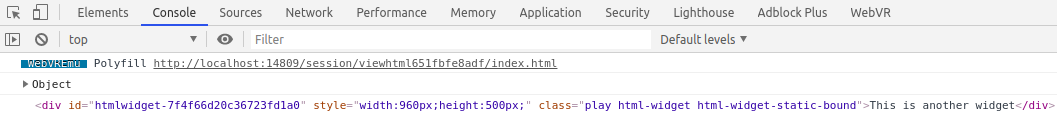
\includegraphics{images/playground-console-el.png}
\caption{Console tab output}
\end{figure}

This displays the HTML element created by htmlwidgets that is meant to hold the visualisation, or in this case, the message. If you are familiar with JavaScript, this is the element that would be returned by \texttt{document.getElementById}. This object allows manipulating the element in pretty much any way imaginable, change its position, its colour, its size, or, as done here, to insert some text within it. What's more one can access attributes of the object just like a JSON array. Therefore one can log the \texttt{id} of the element.

\begin{Shaded}
\begin{Highlighting}[]
\CommentTok{// print the id of the element}
\VariableTok{console}\NormalTok{.}\AttributeTok{log}\NormalTok{(}\VariableTok{el}\NormalTok{.}\AttributeTok{id}\NormalTok{)}\OperatorTok{;}
\VariableTok{el}\NormalTok{.}\AttributeTok{innerText} \OperatorTok{=} \VariableTok{x}\NormalTok{.}\AttributeTok{message}\OperatorTok{;}
\end{Highlighting}
\end{Shaded}

Making the modifications above and reloading the package, one can create a widget given a specific id and see it displayed in the console, e.g.: \texttt{play("hello",\ elementId\ =\ "see-you-in-the-console")}.

In an attempt to become more at ease with this setup let us change something and play with the widget. Out-of-the-box htmlwidgets uses \texttt{innerText}, which does very much what it says on the tin, it places text inside an element. JavaScript comes with another function akin to \texttt{innerText}, \texttt{innerHTML}. While the former only allows inserting text the former lets one insert any HTML.

\begin{Shaded}
\begin{Highlighting}[]
\VariableTok{el}\NormalTok{.}\AttributeTok{innerHTML} \OperatorTok{=} \VariableTok{x}\NormalTok{.}\AttributeTok{message}\OperatorTok{;}
\end{Highlighting}
\end{Shaded}

After changing the \texttt{play.js} file as above, and re-loading the package, one can use arbitrary HTML as messages.

\begin{Shaded}
\begin{Highlighting}[]
\KeywordTok{play}\NormalTok{(}\StringTok{"<h1>Using HTML!</h1>"}\NormalTok{)}
\end{Highlighting}
\end{Shaded}

\begin{figure}
\centering
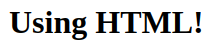
\includegraphics{images/playground-h1.png}
\caption{Widget output}
\end{figure}

That makes for a great improvement which opens the door to many possibilities. However, the interface this provides is unintuitive. Albeit similar, R users are more familiar with shiny and htmltools \citep{R-htmltools} tags than HTML tags, e.g.: \texttt{\textless{}h1\textgreater{}\textless{}/h1\textgreater{}} translates to \texttt{h1()} in R. The package should allow users to use those instead of forcing them to collapse HTML content in a string. Fortunately, there is a very easy way to obtain the HTML from those functions: convert it to a character string.

\begin{Shaded}
\begin{Highlighting}[]
\NormalTok{html <{-}}\StringTok{ }\NormalTok{shiny}\OperatorTok{::}\KeywordTok{h1}\NormalTok{(}\StringTok{"HTML tag"}\NormalTok{)}

\KeywordTok{class}\NormalTok{(html)}
\end{Highlighting}
\end{Shaded}

\begin{verbatim}
## [1] "shiny.tag"
\end{verbatim}

\begin{Shaded}
\begin{Highlighting}[]
\CommentTok{\# returns string}
\KeywordTok{as.character}\NormalTok{(html)}
\end{Highlighting}
\end{Shaded}

\begin{verbatim}
## [1] "<h1>HTML tag</h1>"
\end{verbatim}

Implementing this in the \texttt{play} function will look like this.

\begin{Shaded}
\begin{Highlighting}[]
\CommentTok{\# forward options using x}
\NormalTok{x =}\StringTok{ }\KeywordTok{list}\NormalTok{(}
  \DataTypeTok{message =} \KeywordTok{as.character}\NormalTok{(message)}
\NormalTok{)}
\end{Highlighting}
\end{Shaded}

Reloading the package with \texttt{devtools::load\_all} lets one use shiny tags as the message.

\begin{Shaded}
\begin{Highlighting}[]
\KeywordTok{play}\NormalTok{(shiny}\OperatorTok{::}\KeywordTok{h2}\NormalTok{(}\StringTok{"Chocolate is a colour"}\NormalTok{, }\DataTypeTok{style =} \StringTok{"color:chocolate;"}\NormalTok{))}
\end{Highlighting}
\end{Shaded}

\begin{figure}
\centering

\includegraphics{images/playground-color.png}
\caption{Using shiny tags}
\end{figure}

This hopefully provides some understanding of how htmlwidgets work internally and thereby helps building such packages. To recapitulate, an HTML document is created in which div is placed and given a certain id, this id is also used in a script tag that contains JSON data passed from R so that a JavaScript function we define can read that data in and use it to generate a visual output in a div. However, as much as this section covered, the topic of JavaScript dependencies was not touched, this is approached in the following section where we build another, more interesting widget, which uses an external dependency.

\hypertarget{a-realistic-widget}{%
\chapter{A Realistic Widget}\label{a-realistic-widget}}

In this section we build a package called \texttt{typed}, which wraps the JavaScript library of the same name, \href{https://github.com/mattboldt/typed.js/}{typed.js} that mimics text being typed. This builds upon many things we explored in the playground package.

\begin{Shaded}
\begin{Highlighting}[]
\NormalTok{usethis}\OperatorTok{::}\KeywordTok{create\_package}\NormalTok{(}\StringTok{"typed"}\NormalTok{)}
\NormalTok{htmlwidgets}\OperatorTok{::}\KeywordTok{scaffoldWidget}\NormalTok{(}\StringTok{"typed"}\NormalTok{)}
\end{Highlighting}
\end{Shaded}

As done with candidate libraries, let's take a look at documentation of \href{https://github.com/mattboldt/typed.js/}{typed.js} to see how typed.js works.

\begin{Shaded}
\begin{Highlighting}[]
\DataTypeTok{<!DOCTYPE }\NormalTok{html}\DataTypeTok{>}
\KeywordTok{<html}\OtherTok{ xmlns=}\StringTok{"http://www.w3.org/1999/xhtml"}\OtherTok{ lang=}\StringTok{""}\OtherTok{ xml:lang=}\StringTok{""}\KeywordTok{>}

\KeywordTok{<head>}
  \CommentTok{<!{-}{-} Import library {-}{-}>}
  \KeywordTok{<script}\OtherTok{ src=}\StringTok{"typed.js"}\KeywordTok{></script>}
\KeywordTok{</head>}

\KeywordTok{<body>}
  \CommentTok{<!{-}{-} div to hold visualisation {-}{-}>}
  \KeywordTok{<div}\OtherTok{ class=}\StringTok{"element"}\KeywordTok{></div>}

  \CommentTok{<!{-}{-} Script to create visualisation {-}{-}>}
  \KeywordTok{<script>}
    \KeywordTok{var}\NormalTok{ typed }\OperatorTok{=} \KeywordTok{new} \AttributeTok{Typed}\NormalTok{(}\StringTok{\textquotesingle{}.element\textquotesingle{}}\OperatorTok{,} \OperatorTok{\{}
      \DataTypeTok{strings}\OperatorTok{:}\NormalTok{ [}\StringTok{\textquotesingle{}First sentence.\textquotesingle{}}\OperatorTok{,} \StringTok{\textquotesingle{}And a second sentence.\textquotesingle{}}\NormalTok{]}
    \OperatorTok{\}}\NormalTok{)}\OperatorTok{;}
  \KeywordTok{</script>}
\KeywordTok{</body>}

\KeywordTok{</html>}
\end{Highlighting}
\end{Shaded}

The code above is not very different from what was observed in other libraries: the library is imported, there is a \texttt{\textless{}div\textgreater{}} where the output will be generated, and a script which also takes a selector and a JSON of options.

\hypertarget{dependency}{%
\section{Dependency}\label{dependency}}

Once the package created and the widget scaffold laid down we need to add the JavaScript dependency without which nothing can move forward. The \href{https://github.com/mattboldt/typed.js}{documentation in the README of typed.js} states that it can be imported like so.

\begin{Shaded}
\begin{Highlighting}[]
\KeywordTok{<script}\OtherTok{ src=}\StringTok{"https://cdn.jsdelivr.net/npm/typed.js@2.0.11"}\KeywordTok{></script>}
\end{Highlighting}
\end{Shaded}

First, we will download the dependency, which consists of a single JavaScript file, instead of using the CDN as this ultimately makes the package more robust (more easily reproducible outputs and no requirement for internet connection). Below we place the dependency in a ``typed'' directory within the ``htmlwidgets'' folder.

\begin{Shaded}
\begin{Highlighting}[]
\KeywordTok{dir.create}\NormalTok{(}\StringTok{"./inst/htmlwidgets/typed"}\NormalTok{)}
\NormalTok{cdn <{-}}\StringTok{ "https://cdn.jsdelivr.net/npm/typed.js@2.0.11"}
\KeywordTok{download.file}\NormalTok{(cdn, }\StringTok{"./inst/htmlwidgets/typed/typed.min.js"}\NormalTok{)}
\end{Highlighting}
\end{Shaded}

This produces a directory that looks like this:

\begin{verbatim}
.
├── DESCRIPTION
├── NAMESPACE
├── R
│   └── typed.R
└── inst
    └── htmlwidgets
        ├── typed
        │   └── typed.min.js
        ├── typed.js
        └── typed.yaml
\end{verbatim}

In htmlwidgets packages dependencies are specified in the \texttt{.yml} file located at \texttt{inst/htmlwidgets} which at first contains a commented template.

\begin{Shaded}
\begin{Highlighting}[]
\CommentTok{\# (uncomment to add a dependency)}
\CommentTok{\# dependencies:}
\CommentTok{\#  {-} name:}
\CommentTok{\#    version:}
\CommentTok{\#    src:}
\CommentTok{\#    script:}
\CommentTok{\#    stylesheet:}
\end{Highlighting}
\end{Shaded}

Let's uncomment those lines as instructed at the top of the file and fill it in.

\begin{Shaded}
\begin{Highlighting}[]
\FunctionTok{dependencies}\KeywordTok{:}
\AttributeTok{  }\KeywordTok{{-}}\AttributeTok{ }\FunctionTok{name}\KeywordTok{:}\AttributeTok{ typed.js}
\AttributeTok{    }\FunctionTok{version}\KeywordTok{:}\AttributeTok{ }\FloatTok{2.0.11}
\AttributeTok{    }\FunctionTok{src}\KeywordTok{:}\AttributeTok{ htmlwidgets/typed}
\AttributeTok{    }\FunctionTok{script}\KeywordTok{:}\AttributeTok{ typed.min.js}
\end{Highlighting}
\end{Shaded}

We remove the \texttt{stylesheet} entry as this package does not require any CSS files. The \texttt{src} specifies the path to the directory containing the scripts and stylesheets. This is akin to using the \texttt{system.file} function to return the full path to a file or directory within the package.

\begin{Shaded}
\begin{Highlighting}[]
\NormalTok{devtools}\OperatorTok{::}\KeywordTok{load\_all}\NormalTok{()}
\KeywordTok{system.file}\NormalTok{(}\StringTok{"htmlwidgets/typed"}\NormalTok{, }\DataTypeTok{package =} \StringTok{"typed"}\NormalTok{)                                         }
\CommentTok{\#> "/home/me/packages/typed/inst/htmlwidgets/typed"}
\end{Highlighting}
\end{Shaded}

We should verify that this is correct by using the one R function the package features and check the source code of the output to verify that the typed.js is indeed imported. We thus run \texttt{typed("test")}, open the output in the browser (
\includegraphics{images/open-in-browser.png}) and look at the source code of the page (right click and select ``View page source''). At the top of the page one should see \texttt{typed.min.js} imported, click the link to ensure it correctly points to the dependency.

\begin{Shaded}
\begin{Highlighting}[]
\DataTypeTok{<!DOCTYPE }\NormalTok{html}\DataTypeTok{>}
\KeywordTok{<html>}
\KeywordTok{<head>}
\KeywordTok{<meta}\OtherTok{ charset=}\StringTok{"utf{-}8"}\KeywordTok{/>}
\KeywordTok{<style>}\NormalTok{body\{}\KeywordTok{background{-}color}\NormalTok{:}\ConstantTok{white}\OperatorTok{;}\NormalTok{\}}\KeywordTok{</style>}
\KeywordTok{<script}\OtherTok{ src=}\StringTok{"lib/htmlwidgets{-}1.5.1/htmlwidgets.js"}\KeywordTok{></script>}
\KeywordTok{<script}\OtherTok{ src=}\StringTok{"lib/typed.js{-}2.0.11/typed.min.js"}\KeywordTok{></script>}
\KeywordTok{<script}\OtherTok{ src=}\StringTok{"lib/typed{-}binding{-}0.0.0.9000/typed.js"}\KeywordTok{></script>}
\NormalTok{...}
\end{Highlighting}
\end{Shaded}

\hypertarget{javascript}{%
\section{JavaScript}\label{javascript}}

On its \href{https://mattboldt.com/demos/typed-js/}{official website}, typed.js gives the following example. The JavaScript function \texttt{Typed} takes two arguments, first the selector, the element to hold the output, second a JSON of options to specify what is being typed and a myriad of other things.

\begin{Shaded}
\begin{Highlighting}[]
\KeywordTok{var}\NormalTok{ typed }\OperatorTok{=} \KeywordTok{new} \AttributeTok{Typed}\NormalTok{(}\StringTok{\textquotesingle{}.element\textquotesingle{}}\OperatorTok{,} \OperatorTok{\{}
  \DataTypeTok{strings}\OperatorTok{:}\NormalTok{ [}\StringTok{"First sentence."}\OperatorTok{,} \StringTok{"Second sentence."}\NormalTok{]}\OperatorTok{,}
  \DataTypeTok{typeSpeed}\OperatorTok{:} \DecValTok{30}
\OperatorTok{\}}\NormalTok{)}\OperatorTok{;}
\end{Highlighting}
\end{Shaded}

Let's place it in the package by replacing the content of the \texttt{renderValue} in \texttt{typed.js} with the above.

\begin{Shaded}
\begin{Highlighting}[]
\NormalTok{...}
\NormalTok{renderValue}\OperatorTok{:} \KeywordTok{function}\NormalTok{(x) }\OperatorTok{\{}

  \KeywordTok{var}\NormalTok{ typed }\OperatorTok{=} \KeywordTok{new} \AttributeTok{Typed}\NormalTok{(}\StringTok{\textquotesingle{}.element\textquotesingle{}}\OperatorTok{,} \OperatorTok{\{}
    \DataTypeTok{strings}\OperatorTok{:}\NormalTok{ [}\StringTok{"First sentence."}\OperatorTok{,} \StringTok{"Second sentence."}\NormalTok{]}\OperatorTok{,}
    \DataTypeTok{typeSpeed}\OperatorTok{:} \DecValTok{30}
  \OperatorTok{\}}\NormalTok{)}\OperatorTok{;}

\OperatorTok{\}}
\NormalTok{...}
\end{Highlighting}
\end{Shaded}

One could be tempted to run \texttt{devtools::load\_all} but this will not work, namely because the function uses a selector that is will not return any object; it needs to be applied to the div created by the widget not \texttt{.element}. As hinted at in the playground, the selector of the element created is accessible from the \texttt{el} object. As a matter of fact, we did log in the browser console the id of the created div taken from \texttt{el.id}. Therefore concatenating the pound sign and the element id produces the select to said element. (\texttt{.class}, \texttt{\#id})

\begin{Shaded}
\begin{Highlighting}[]
\CommentTok{// typed.js}
\NormalTok{...}
\NormalTok{renderValue}\OperatorTok{:} \KeywordTok{function}\NormalTok{(x) }\OperatorTok{\{}

  \KeywordTok{var}\NormalTok{ typed }\OperatorTok{=} \KeywordTok{new} \AttributeTok{Typed}\NormalTok{(}\StringTok{\textquotesingle{}\#\textquotesingle{}} \OperatorTok{+} \VariableTok{el}\NormalTok{.}\AttributeTok{id}\OperatorTok{,} \OperatorTok{\{}
    \DataTypeTok{strings}\OperatorTok{:}\NormalTok{ [}\StringTok{"First sentence."}\OperatorTok{,} \StringTok{"Second sentence."}\NormalTok{]}\OperatorTok{,}
    \DataTypeTok{typeSpeed}\OperatorTok{:} \DecValTok{30}
  \OperatorTok{\}}\NormalTok{)}\OperatorTok{;}

\OperatorTok{\}}
\NormalTok{...}
\end{Highlighting}
\end{Shaded}

This should now work, run \texttt{devtools::load\_all} followed by \texttt{typed("whatever")} and the JavaScript animated text will appear! It's not of any use just yet as the options, including the text being typed is predefined: the package is currently not making any use the of the inputs passed from R. This can be changed by using \texttt{x.message} passed from R instead of the default strings.

\begin{Shaded}
\begin{Highlighting}[]
\CommentTok{// typed.js}
\NormalTok{...}
\NormalTok{renderValue}\OperatorTok{:} \KeywordTok{function}\NormalTok{(x) }\OperatorTok{\{}

  \KeywordTok{var}\NormalTok{ typed }\OperatorTok{=} \KeywordTok{new} \AttributeTok{Typed}\NormalTok{(}\StringTok{\textquotesingle{}\#\textquotesingle{}} \OperatorTok{+} \VariableTok{el}\NormalTok{.}\AttributeTok{id}\OperatorTok{,} \OperatorTok{\{}
    \DataTypeTok{strings}\OperatorTok{:} \VariableTok{x}\NormalTok{.}\AttributeTok{message}\OperatorTok{,}
    \DataTypeTok{typeSpeed}\OperatorTok{:} \DecValTok{30}
  \OperatorTok{\}}\NormalTok{)}\OperatorTok{;}

\OperatorTok{\}}
\NormalTok{...}
\end{Highlighting}
\end{Shaded}

This, however, will cause issues as the \texttt{strings} options expects and array (vector) and not a single string.

\begin{Shaded}
\begin{Highlighting}[]
\KeywordTok{typed}\NormalTok{(}\StringTok{"does not work"}\NormalTok{) }\CommentTok{\# length =  1}
\KeywordTok{typed}\NormalTok{(}\KeywordTok{c}\NormalTok{(}\StringTok{"This"}\NormalTok{, }\StringTok{"will"}\NormalTok{, }\StringTok{"work"}\NormalTok{)) }\CommentTok{\# length > 1}
\end{Highlighting}
\end{Shaded}

One solution is to force the input into a list.

\begin{Shaded}
\begin{Highlighting}[]
\CommentTok{\# typed.R}
\NormalTok{x =}\StringTok{ }\KeywordTok{list}\NormalTok{(}
  \DataTypeTok{message =} \KeywordTok{as.list}\NormalTok{(message)}
\NormalTok{)}
\end{Highlighting}
\end{Shaded}

At this juncture the package works but there is a salient issue with the way it handles options. Why build a list in R to reconstruct it in JavaScript manually. Since the options are serialised in R to JSON and that typed.js expects a JSON of options it is actually cleaner and more convenient to construct an R list that mirrors the JSON array so one can use it as-is in JavaScript.

In fact, renaming the \texttt{message} to \texttt{strings} effectively does this.

\begin{Shaded}
\begin{Highlighting}[]
\CommentTok{\# typed.R}
\NormalTok{x =}\StringTok{ }\KeywordTok{list}\NormalTok{(}
  \DataTypeTok{strings =} \KeywordTok{as.list}\NormalTok{(message)}
\NormalTok{)}
\end{Highlighting}
\end{Shaded}

This allows greatly simplifying the code JavaScript side, making it much easier to add other options down the line, maintain, debug, and read.

\begin{Shaded}
\begin{Highlighting}[]
\CommentTok{// typed.js}
\NormalTok{...}
\NormalTok{renderValue}\OperatorTok{:} \KeywordTok{function}\NormalTok{(x) }\OperatorTok{\{}

  \KeywordTok{var}\NormalTok{ typed }\OperatorTok{=} \KeywordTok{new} \AttributeTok{Typed}\NormalTok{(}\StringTok{\textquotesingle{}\#\textquotesingle{}} \OperatorTok{+} \VariableTok{el}\NormalTok{.}\AttributeTok{id}\OperatorTok{,}\NormalTok{ x)}\OperatorTok{;}

\OperatorTok{\}}
\NormalTok{...}
\end{Highlighting}
\end{Shaded}

One can now add more options from the R code without having to alter any of the JavaScript. Let us demonstrate with the \texttt{loop} option.

\begin{Shaded}
\begin{Highlighting}[]
\NormalTok{typed <{-}}\StringTok{ }\ControlFlowTok{function}\NormalTok{(message, }\DataTypeTok{loop =} \OtherTok{FALSE}\NormalTok{, }
  \DataTypeTok{width =} \OtherTok{NULL}\NormalTok{, }\DataTypeTok{height =} \OtherTok{NULL}\NormalTok{, }\DataTypeTok{elementId =} \OtherTok{NULL}\NormalTok{) \{}

  \CommentTok{\# forward options using x}
\NormalTok{  x =}\StringTok{ }\KeywordTok{list}\NormalTok{(}
    \DataTypeTok{loop =}\NormalTok{ loop,}
    \DataTypeTok{strings =} \KeywordTok{as.list}\NormalTok{(message)}
\NormalTok{  )}

  \CommentTok{\# create widget}
\NormalTok{  htmlwidgets}\OperatorTok{::}\KeywordTok{createWidget}\NormalTok{(}
    \DataTypeTok{name =} \StringTok{\textquotesingle{}typed\textquotesingle{}}\NormalTok{,}
\NormalTok{    x,}
    \DataTypeTok{width =}\NormalTok{ width,}
    \DataTypeTok{height =}\NormalTok{ height,}
    \DataTypeTok{package =} \StringTok{\textquotesingle{}typed\textquotesingle{}}\NormalTok{,}
    \DataTypeTok{elementId =}\NormalTok{ elementId}
\NormalTok{  )}
\NormalTok{\}}
\end{Highlighting}
\end{Shaded}

\hypertarget{html-element}{%
\section{HTML Element}\label{html-element}}

As pointed out multiple times, the widget is generated in a \texttt{\textless{}div\textgreater{}}, which is works fine for most visualisation libraries. But we saw that chart.js requires placing it in a \texttt{\textless{}canvas\textgreater{}}, so one needs the ability to change that. It could be interesting to apply this to typed.js too as within a \texttt{\textless{}div\textgreater{}} it cannot be placed inline, using a \texttt{\textless{}span\textgreater{}}, however, this would work.

This can be changed by placing a function named \texttt{nameOfWidget\_html} which looked up by htmlwidgets and used if found. This function takes the three-dot construct \texttt{...} and uses them in an htmltools tag. The three-dots are necessary because internally htmlwidgets needs be able to pass arguments, such as the all too critical \texttt{id}.

\begin{Shaded}
\begin{Highlighting}[]
\NormalTok{typed\_html <{-}}\StringTok{ }\ControlFlowTok{function}\NormalTok{(...)\{}
\NormalTok{  htmltools}\OperatorTok{::}\NormalTok{tags}\OperatorTok{$}\KeywordTok{span}\NormalTok{(...)}
\NormalTok{\}}
\end{Highlighting}
\end{Shaded}

Note that this can also be used to force certain attributes onto the element. For instance we could use the code below to force all output to use a red font.

\begin{Shaded}
\begin{Highlighting}[]
\NormalTok{typed\_html <{-}}\StringTok{ }\ControlFlowTok{function}\NormalTok{(...)\{}
\NormalTok{  htmltools}\OperatorTok{::}\NormalTok{tags}\OperatorTok{$}\KeywordTok{span}\NormalTok{(..., }\DataTypeTok{style =} \StringTok{"color:red;"}\NormalTok{)}
\NormalTok{\}}
\end{Highlighting}
\end{Shaded}

We shall leave it at that and move on to building another widget but completing the package makes for an interesting exercise.

\hypertarget{the-full-monty}{%
\chapter{The Full Monty}\label{the-full-monty}}

With a first widget built one can jump onto another one: \href{https://giojs.org/}{gio.js}, a library to draw arcs between countries on a 3 dimensional globe. This will include many more functionalities such packages can comprise.

Then again, the first order of business when looking to integrate a library is to look at the documentation to understand what should be reproduced in R.

\begin{Shaded}
\begin{Highlighting}[]
\DataTypeTok{<!DOCTYPE }\NormalTok{html}\DataTypeTok{>}
\KeywordTok{<html}\OtherTok{ xmlns=}\StringTok{"http://www.w3.org/1999/xhtml"}\OtherTok{ lang=}\StringTok{""}\OtherTok{ xml:lang=}\StringTok{""}\KeywordTok{>}

\KeywordTok{<head>}
  \CommentTok{<!{-}{-} Import libraries {-}{-}>}
  \KeywordTok{<script}\OtherTok{ src=}\StringTok{"three.min.js"}\KeywordTok{></script>}
  \KeywordTok{<script}\OtherTok{ src=}\StringTok{"gio.min.js"}\KeywordTok{></script>}
\KeywordTok{</head>}

\KeywordTok{<body>}
  \CommentTok{<!{-}{-} div to hold visualisation {-}{-}>}
  \KeywordTok{<div}\OtherTok{ id=}\StringTok{"globe"}\OtherTok{ style=}\StringTok{"width: 200px; height: 200px"}\KeywordTok{></div>}

  \CommentTok{<!{-}{-} Script to create visualisation {-}{-}>}
  \KeywordTok{<script>}
    \KeywordTok{var}\NormalTok{ container }\OperatorTok{=} \VariableTok{document}\NormalTok{.}\AttributeTok{getElementById}\NormalTok{(}\StringTok{"globe"}\NormalTok{)}\OperatorTok{;}
    \KeywordTok{var}\NormalTok{ controller }\OperatorTok{=} \KeywordTok{new} \VariableTok{GIO}\NormalTok{.}\AttributeTok{Controller}\NormalTok{(container)}\OperatorTok{;}
    \VariableTok{controller}\NormalTok{.}\AttributeTok{addData}\NormalTok{(data)}\OperatorTok{;}
    \VariableTok{controller}\NormalTok{.}\AttributeTok{init}\NormalTok{()}\OperatorTok{;}
  \KeywordTok{</script>}
\KeywordTok{</body>}

\KeywordTok{</html>}
\end{Highlighting}
\end{Shaded}

\begin{figure}
\centering
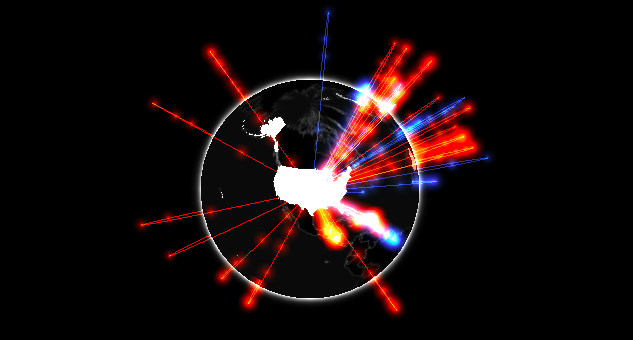
\includegraphics{images/gio-example.png}
\caption{Example of Gio.js visualisation}
\end{figure}

Gio.js has itself a dependency, \href{https://threejs.org/}{three.js}, which needs to be imported before gio.js, other than that not much differs from libraries previously explored in this chapter.

\begin{Shaded}
\begin{Highlighting}[]
\NormalTok{usethis}\OperatorTok{::}\KeywordTok{create\_package}\NormalTok{(}\StringTok{"gio"}\NormalTok{)}
\NormalTok{htmlwidgets}\OperatorTok{::}\KeywordTok{scaffoldWidget}\NormalTok{(}\StringTok{"gio"}\NormalTok{)}
\end{Highlighting}
\end{Shaded}

\hypertarget{dependencies}{%
\section{Dependencies}\label{dependencies}}

Handling the dependencies does not differ much, we only need to download two libraries instead of one.

\begin{Shaded}
\begin{Highlighting}[]
\CommentTok{\# create directories for JS dependencies}
\KeywordTok{dir.create}\NormalTok{(}\StringTok{"./inst/htmlwidgets/three"}\NormalTok{, }\DataTypeTok{recursive =} \OtherTok{TRUE}\NormalTok{)}
\KeywordTok{dir.create}\NormalTok{(}\StringTok{"./inst/htmlwidgets/gio"}\NormalTok{, }\DataTypeTok{recursive =} \OtherTok{TRUE}\NormalTok{)}

\CommentTok{\# download JS dependencies}
\NormalTok{three <{-}}\StringTok{ }\KeywordTok{paste0}\NormalTok{(}
  \StringTok{"https://cdnjs.cloudflare.com/ajax/"}\NormalTok{,}
  \StringTok{"libs/three.js/110/three.min.js"}
\NormalTok{)}
\NormalTok{gio <{-}}\StringTok{ }\KeywordTok{paste0}\NormalTok{(}
  \StringTok{"https://raw.githubusercontent.com/"}\NormalTok{,}
  \StringTok{"syt123450/giojs/master/build/gio.min.js"}
\NormalTok{)}

\KeywordTok{download.file}\NormalTok{(three, }\StringTok{"./inst/htmlwidgets/three/three.min.js"}\NormalTok{)}
\KeywordTok{download.file}\NormalTok{(gio, }\StringTok{"./inst/htmlwidgets/gio/gio.min.js"}\NormalTok{)}
\end{Highlighting}
\end{Shaded}

This should produce the following working directory.

\begin{verbatim}
.
├── DESCRIPTION
├── NAMESPACE
├── R
│   └── gio.R
└── inst
    └── htmlwidgets
        ├── gio
        │   └── gio.min.js
        ├── gio.js
        ├── gio.yaml
        └── three
            └── three.min.js
\end{verbatim}

The libraries have been downloaded but the \texttt{gio.yml} file is yet to be edited. The order in which the libraries are listed matters; just as in HTML three.js needs to precede gio.js as the latter depends on the former and not vice versa.

\begin{Shaded}
\begin{Highlighting}[]
\FunctionTok{dependencies}\KeywordTok{:}
\AttributeTok{  }\KeywordTok{{-}}\AttributeTok{ }\FunctionTok{name}\KeywordTok{:}\AttributeTok{ three}
\AttributeTok{    }\FunctionTok{version}\KeywordTok{:}\AttributeTok{ }\DecValTok{110}
\AttributeTok{    }\FunctionTok{src}\KeywordTok{:}\AttributeTok{ htmlwidgets/three}
\AttributeTok{    }\FunctionTok{script}\KeywordTok{:}\AttributeTok{ three.min.js}
\AttributeTok{  }\KeywordTok{{-}}\AttributeTok{ }\FunctionTok{name}\KeywordTok{:}\AttributeTok{ gio}
\AttributeTok{    }\FunctionTok{version}\KeywordTok{:}\AttributeTok{ }\FloatTok{2.0}
\AttributeTok{    }\FunctionTok{src}\KeywordTok{:}\AttributeTok{ htmlwidgets/gio}
\AttributeTok{    }\FunctionTok{script}\KeywordTok{:}\AttributeTok{ gio.min.js}
\end{Highlighting}
\end{Shaded}

\hypertarget{javascript}{%
\section{JavaScript}\label{javascript}}

Let's copy the JavaScript code from the \href{https://giojs.org/index.html}{Get Started section of gio.js} in the \texttt{gio.js} file's \texttt{renderValue} function. At this point the data format is not known so we comment the line which adds data to the visualisation.

\begin{Shaded}
\begin{Highlighting}[]
\CommentTok{// gio.js}
\VariableTok{HTMLWidgets}\NormalTok{.}\AttributeTok{widget}\NormalTok{(}\OperatorTok{\{}

  \DataTypeTok{name}\OperatorTok{:} \StringTok{\textquotesingle{}gio\textquotesingle{}}\OperatorTok{,}

  \DataTypeTok{type}\OperatorTok{:} \StringTok{\textquotesingle{}output\textquotesingle{}}\OperatorTok{,}

  \DataTypeTok{factory}\OperatorTok{:} \KeywordTok{function}\NormalTok{(el}\OperatorTok{,}\NormalTok{ width}\OperatorTok{,}\NormalTok{ height) }\OperatorTok{\{}

    \CommentTok{// }\AlertTok{TODO}\CommentTok{: define shared variables for this instance}

    \ControlFlowTok{return} \OperatorTok{\{}

      \DataTypeTok{renderValue}\OperatorTok{:} \KeywordTok{function}\NormalTok{(x) }\OperatorTok{\{}

        \KeywordTok{var}\NormalTok{ container }\OperatorTok{=} \VariableTok{document}\NormalTok{.}\AttributeTok{getElementById}\NormalTok{(}\StringTok{"globe"}\NormalTok{)}\OperatorTok{;}
        \KeywordTok{var}\NormalTok{ controller }\OperatorTok{=} \KeywordTok{new} \VariableTok{GIO}\NormalTok{.}\AttributeTok{Controller}\NormalTok{(container)}\OperatorTok{;}
        \CommentTok{//controller.addData(data);}
        \VariableTok{controller}\NormalTok{.}\AttributeTok{init}\NormalTok{()}\OperatorTok{;}

      \OperatorTok{\},}

      \DataTypeTok{resize}\OperatorTok{:} \KeywordTok{function}\NormalTok{(width}\OperatorTok{,}\NormalTok{ height) }\OperatorTok{\{}

        \CommentTok{// }\AlertTok{TODO}\CommentTok{: code to re{-}render the widget with a new size}

      \OperatorTok{\}}

    \OperatorTok{\};}
  \OperatorTok{\}}
\OperatorTok{\}}\NormalTok{)}\OperatorTok{;}
\end{Highlighting}
\end{Shaded}

One can document and load the package but it will not work as the code above attempts to place the visualisation in a \texttt{div} with \texttt{id\ =\ "globe"}. As for the previously written widget, this needs to be changed to \texttt{el.id}.

\begin{Shaded}
\begin{Highlighting}[]
\CommentTok{// gio.js}
\NormalTok{renderValue}\OperatorTok{:} \KeywordTok{function}\NormalTok{(x) }\OperatorTok{\{}

  \KeywordTok{var}\NormalTok{ container }\OperatorTok{=} \VariableTok{document}\NormalTok{.}\AttributeTok{getElementById}\NormalTok{(}\VariableTok{el}\NormalTok{.}\AttributeTok{id}\NormalTok{)}\OperatorTok{;}
  \KeywordTok{var}\NormalTok{ controller }\OperatorTok{=} \KeywordTok{new} \VariableTok{GIO}\NormalTok{.}\AttributeTok{Controller}\NormalTok{(container)}\OperatorTok{;}
  \CommentTok{//controller.addData(data);}
  \VariableTok{controller}\NormalTok{.}\AttributeTok{init}\NormalTok{()}\OperatorTok{;}

\OperatorTok{\}}
\end{Highlighting}
\end{Shaded}

At this stage the widget should generate a visualisation.

\begin{Shaded}
\begin{Highlighting}[]
\NormalTok{devtools}\OperatorTok{::}\KeywordTok{document}\NormalTok{()}
\NormalTok{devtools}\OperatorTok{::}\KeywordTok{load\_all}\NormalTok{()}
\KeywordTok{gio}\NormalTok{(}\DataTypeTok{message =} \StringTok{"This required but not used"}\NormalTok{)}
\end{Highlighting}
\end{Shaded}

\begin{figure}
\centering

\includegraphics{images/gio-init.png}
\caption{Output without data}
\end{figure}

Not too shabby given how little work was put into this! Before we move on let us optimise something. In the JavaScript code we retrieve the \texttt{container} using \texttt{el.id} but this in effect is very inefficient: \texttt{el} is identical to \texttt{container}.

\begin{Shaded}
\begin{Highlighting}[]
\CommentTok{// gio.js}
\NormalTok{renderValue}\OperatorTok{:} \KeywordTok{function}\NormalTok{(x) }\OperatorTok{\{}

  \KeywordTok{var}\NormalTok{ controller }\OperatorTok{=} \KeywordTok{new} \VariableTok{GIO}\NormalTok{.}\AttributeTok{Controller}\NormalTok{(el)}\OperatorTok{;}
  \CommentTok{//controller.addData(data);}
  \VariableTok{controller}\NormalTok{.}\AttributeTok{init}\NormalTok{()}\OperatorTok{;}

\OperatorTok{\}}
\end{Highlighting}
\end{Shaded}

\hypertarget{working-with-data}{%
\section{Working with Data}\label{working-with-data}}

An interesting start, now onto adding data. Let's take a look at the \href{https://giojs.org/html/docs/dataAdd.html}{documentation} to see what data the library expects.

\begin{Shaded}
\begin{Highlighting}[]
\OtherTok{[}
  \FunctionTok{\{}
    \DataTypeTok{"e"}\FunctionTok{:} \StringTok{"CN"}\FunctionTok{,}
    \DataTypeTok{"i"}\FunctionTok{:} \StringTok{"US"}\FunctionTok{,}
    \DataTypeTok{"v"}\FunctionTok{:} \DecValTok{3300000}
  \FunctionTok{\}}\OtherTok{,}
  \FunctionTok{\{}
    \DataTypeTok{"e"}\FunctionTok{:} \StringTok{"CN"}\FunctionTok{,}
    \DataTypeTok{"i"}\FunctionTok{:} \StringTok{"RU"}\FunctionTok{,}
    \DataTypeTok{"v"}\FunctionTok{:} \DecValTok{10000}
  \FunctionTok{\}}
\OtherTok{]}
\end{Highlighting}
\end{Shaded}

The JSON data should constitutes of arrays that denote arcs to draw on the globe where each arc is defined by an exporting country (\texttt{e}), an importing country (\texttt{i}), and is given a value (\texttt{v}). The importing and exporting country, the source and target of the arc, are indicated by ISO alpha-2 country codes. We can read this JSON into R.

\begin{Shaded}
\begin{Highlighting}[]
\CommentTok{\# data.frame to test}
\NormalTok{arcs <{-}}\StringTok{ }\NormalTok{jsonlite}\OperatorTok{::}\KeywordTok{fromJSON}\NormalTok{(}
  \StringTok{\textquotesingle{}[}
\StringTok{    \{}
\StringTok{      "e": "CN",}
\StringTok{      "i": "US",}
\StringTok{      "v": 3300000}
\StringTok{    \},}
\StringTok{    \{}
\StringTok{      "e": "CN",}
\StringTok{      "i": "RU",}
\StringTok{      "v": 10000}
\StringTok{    \}}
\StringTok{  ]\textquotesingle{}}
\NormalTok{)}

\KeywordTok{print}\NormalTok{(arcs)}
\end{Highlighting}
\end{Shaded}

\begin{verbatim}
##    e  i       v
## 1 CN US 3300000
## 2 CN RU   10000
\end{verbatim}

Jsonlite automagically converts the JSON into a data frame where each row is an arc, which is great as R users tend to prefer rectangular data over lists: this is probably what the package should use as input too. Let us make some changes to the \texttt{gio} function so it takes data as input.

\begin{Shaded}
\begin{Highlighting}[]
\NormalTok{gio <{-}}\StringTok{ }\ControlFlowTok{function}\NormalTok{(data, }\DataTypeTok{width =} \OtherTok{NULL}\NormalTok{, }\DataTypeTok{height =} \OtherTok{NULL}\NormalTok{, }\DataTypeTok{elementId =} \OtherTok{NULL}\NormalTok{) \{}

  \CommentTok{\# forward options using x}
\NormalTok{  x =}\StringTok{ }\KeywordTok{list}\NormalTok{(}
    \DataTypeTok{data =}\NormalTok{ data}
\NormalTok{  )}

  \CommentTok{\# create widget}
\NormalTok{  htmlwidgets}\OperatorTok{::}\KeywordTok{createWidget}\NormalTok{(}
    \DataTypeTok{name =} \StringTok{\textquotesingle{}gio\textquotesingle{}}\NormalTok{,}
\NormalTok{    x,}
    \DataTypeTok{width =}\NormalTok{ width,}
    \DataTypeTok{height =}\NormalTok{ height,}
    \DataTypeTok{package =} \StringTok{\textquotesingle{}gio\textquotesingle{}}\NormalTok{,}
    \DataTypeTok{elementId =}\NormalTok{ elementId}
\NormalTok{  )}
\NormalTok{\}}
\end{Highlighting}
\end{Shaded}

This must be reflected in the \texttt{play.js} file where we uncomment the line previously commented and use \texttt{x.data} passed from R.

\begin{Shaded}
\begin{Highlighting}[]
\CommentTok{// gio.js}
\NormalTok{renderValue}\OperatorTok{:} \KeywordTok{function}\NormalTok{(x) }\OperatorTok{\{}

  \KeywordTok{var}\NormalTok{ controller }\OperatorTok{=} \KeywordTok{new} \VariableTok{GIO}\NormalTok{.}\AttributeTok{Controller}\NormalTok{(el)}\OperatorTok{;}
  \VariableTok{controller}\NormalTok{.}\AttributeTok{addData}\NormalTok{(}\VariableTok{x}\NormalTok{.}\AttributeTok{data}\NormalTok{)}\OperatorTok{;} \CommentTok{// uncomment \& use x.data}
  \VariableTok{controller}\NormalTok{.}\AttributeTok{init}\NormalTok{()}\OperatorTok{;}

\OperatorTok{\}}
\end{Highlighting}
\end{Shaded}

We can now use the function with the data to plot arcs!

\begin{Shaded}
\begin{Highlighting}[]
\NormalTok{devtools}\OperatorTok{::}\KeywordTok{document}\NormalTok{()}
\NormalTok{devtools}\OperatorTok{::}\KeywordTok{load\_all}\NormalTok{()}
\KeywordTok{gio}\NormalTok{(arcs)}
\end{Highlighting}
\end{Shaded}

Unfortunately, this breaks everything and we are presented with a blank screen. Using \texttt{console.log} or looking at the source code the rendered widget reveals the problem: the data isn't actually in the correct format!

\begin{Shaded}
\begin{Highlighting}[]
\FunctionTok{\{}\DataTypeTok{"x"}\FunctionTok{:\{}\DataTypeTok{"data"}\FunctionTok{:\{}\DataTypeTok{"e"}\FunctionTok{:}\OtherTok{[}\StringTok{"CN"}\OtherTok{,}\StringTok{"CN"}\OtherTok{]}\FunctionTok{,}\DataTypeTok{"i"}\FunctionTok{:}\OtherTok{[}\StringTok{"US"}\OtherTok{,}\StringTok{"RU"}\OtherTok{]}\FunctionTok{,}\DataTypeTok{"v"}\FunctionTok{:}\OtherTok{[}\DecValTok{3300000}\OtherTok{,}\DecValTok{10000}\OtherTok{]}\FunctionTok{\}\},}\DataTypeTok{"evals"}\FunctionTok{:}\OtherTok{[]}\FunctionTok{,}\DataTypeTok{"jsHooks"}\FunctionTok{:}\OtherTok{[]}\FunctionTok{\}}
\end{Highlighting}
\end{Shaded}

Htmlwidgets actually serialised the data frame column-wise (long) where each array is a column, whereas gio.js expect the data to be wide (row-wise serialisation) where each array is a arc (row).

\begin{Shaded}
\begin{Highlighting}[]
\CommentTok{\# column{-}wise}
\NormalTok{jsonlite}\OperatorTok{::}\KeywordTok{toJSON}\NormalTok{(arcs, }\DataTypeTok{dataframe =} \StringTok{"columns"}\NormalTok{)}
\end{Highlighting}
\end{Shaded}

\begin{verbatim}
## {"e":["CN","CN"],"i":["US","RU"],"v":[3300000,10000]}
\end{verbatim}

\begin{Shaded}
\begin{Highlighting}[]
\CommentTok{\# row{-}wise}
\NormalTok{jsonlite}\OperatorTok{::}\KeywordTok{toJSON}\NormalTok{(arcs, }\DataTypeTok{dataframe =} \StringTok{"rows"}\NormalTok{)}
\end{Highlighting}
\end{Shaded}

\begin{verbatim}
## [{"e":"CN","i":"US","v":3300000},{"e":"CN","i":"RU","v":10000}]
\end{verbatim}

As mentioned previously, convention has it that rectangular data (data frames) are serialised row-wise. This is likely to be a recurring problem.

\hypertarget{transforming-data}{%
\section{Transforming Data}\label{transforming-data}}

There are multiple ways to transform the data and ensure the serialised JSON is as the JavaScript library expects it to be.

\hypertarget{in-javascript}{%
\subsection{In JavaScript}\label{in-javascript}}

JavaScript can be used to transform the data, leaving the serialiser as-is to reshape the data in the client. The HTMLwidget JavaScript library (already imported by default) exports an object which provides a method, \texttt{dataframeToD3}, to transform the data from long to wide.

\begin{Shaded}
\begin{Highlighting}[]
\CommentTok{// gio.js}
\NormalTok{renderValue}\OperatorTok{:} \KeywordTok{function}\NormalTok{(x) }\OperatorTok{\{}

  \CommentTok{// long to wide}
  \VariableTok{x}\NormalTok{.}\AttributeTok{data} \OperatorTok{=} \VariableTok{HTMLWidgets}\NormalTok{.}\AttributeTok{dataframeToD3}\NormalTok{(}\VariableTok{x}\NormalTok{.}\AttributeTok{data}\NormalTok{)}\OperatorTok{;}

  \KeywordTok{var}\NormalTok{ controller }\OperatorTok{=} \KeywordTok{new} \VariableTok{GIO}\NormalTok{.}\AttributeTok{Controller}\NormalTok{(el)}\OperatorTok{;}
  \VariableTok{controller}\NormalTok{.}\AttributeTok{addData}\NormalTok{(}\VariableTok{x}\NormalTok{.}\AttributeTok{data}\NormalTok{)}\OperatorTok{;} 
  \VariableTok{controller}\NormalTok{.}\AttributeTok{init}\NormalTok{()}\OperatorTok{;}

\OperatorTok{\}}
\end{Highlighting}
\end{Shaded}

\hypertarget{in-r}{%
\subsection{In R}\label{in-r}}

Instead of serialising the data a certain way then correct in JavaScript as demonstrated previously, one can also modify, or even replace, htmlwidgets' default serialiser. Speaking of which, below is the default serializer used by htmlwidgets.

\begin{Shaded}
\begin{Highlighting}[]
\ControlFlowTok{function}\NormalTok{ (x, ..., }\DataTypeTok{dataframe =} \StringTok{"columns"}\NormalTok{, }\DataTypeTok{null =} \StringTok{"null"}\NormalTok{, }
\DataTypeTok{na =} \StringTok{"null"}\NormalTok{, }\DataTypeTok{auto\_unbox =} \OtherTok{TRUE}\NormalTok{, }\DataTypeTok{use\_signif =} \OtherTok{TRUE}\NormalTok{, }
  \DataTypeTok{digits =} \KeywordTok{getOption}\NormalTok{(}\StringTok{"shiny.json.digits"}\NormalTok{, }\DecValTok{16}\NormalTok{), }\DataTypeTok{force =} \OtherTok{TRUE}\NormalTok{,}
  \DataTypeTok{POSIXt =} \StringTok{"ISO8601"}\NormalTok{, }\DataTypeTok{UTC =} \OtherTok{TRUE}\NormalTok{, }\DataTypeTok{rownames =} \OtherTok{FALSE}\NormalTok{, }
  \DataTypeTok{keep\_vec\_names =} \OtherTok{TRUE}\NormalTok{, }\DataTypeTok{strict\_atomic =} \OtherTok{TRUE}\NormalTok{) }
\NormalTok{\{}
  \ControlFlowTok{if}\NormalTok{ (strict\_atomic) }
\NormalTok{      x <{-}}\StringTok{ }\KeywordTok{I}\NormalTok{(x)}
\NormalTok{  jsonlite}\OperatorTok{::}\KeywordTok{toJSON}\NormalTok{(x, }\DataTypeTok{dataframe =}\NormalTok{ dataframe, }\DataTypeTok{null =}\NormalTok{ null, }\DataTypeTok{na =}\NormalTok{ na, }
    \DataTypeTok{auto\_unbox =}\NormalTok{ auto\_unbox, }\DataTypeTok{digits =}\NormalTok{ digits, }\DataTypeTok{force =}\NormalTok{ force, }
    \DataTypeTok{use\_signif =}\NormalTok{ use\_signif, }\DataTypeTok{POSIXt =}\NormalTok{ POSIXt, }\DataTypeTok{UTC =}\NormalTok{ UTC, }
    \DataTypeTok{rownames =}\NormalTok{ rownames, }\DataTypeTok{keep\_vec\_names =}\NormalTok{ keep\_vec\_names, }
    \DataTypeTok{json\_verbatim =} \OtherTok{TRUE}\NormalTok{, ...)}
\NormalTok{\}}
\end{Highlighting}
\end{Shaded}

The problem at hand is caused by the \texttt{dataframe} argument which is set to \texttt{columns} where it should be set \texttt{rows} (for row-wise). Arguments are passed to the serialiser indirectly, in the form of a list set as \texttt{TOJSON\_ARGS} attribute to the object \texttt{x} that is serialised. We could thus change the \texttt{gio} function to reflect the aforementioned change.

\begin{Shaded}
\begin{Highlighting}[]
\NormalTok{gio <{-}}\StringTok{ }\ControlFlowTok{function}\NormalTok{(data, }\DataTypeTok{width =} \OtherTok{NULL}\NormalTok{, }\DataTypeTok{height =} \OtherTok{NULL}\NormalTok{, }
  \DataTypeTok{elementId =} \OtherTok{NULL}\NormalTok{) \{}

  \CommentTok{\# forward options using x}
\NormalTok{  x =}\StringTok{ }\KeywordTok{list}\NormalTok{(}
    \DataTypeTok{data =}\NormalTok{ data}
\NormalTok{  )}

  \CommentTok{\# serialise data.frames to wide (not long as default)}
  \KeywordTok{attr}\NormalTok{(x, }\StringTok{\textquotesingle{}TOJSON\_ARGS\textquotesingle{}}\NormalTok{) <{-}}\StringTok{ }\KeywordTok{list}\NormalTok{(}\DataTypeTok{dataframe =} \StringTok{"rows"}\NormalTok{)}

  \CommentTok{\# create widget}
\NormalTok{  htmlwidgets}\OperatorTok{::}\KeywordTok{createWidget}\NormalTok{(}
    \DataTypeTok{name =} \StringTok{\textquotesingle{}gio\textquotesingle{}}\NormalTok{,}
\NormalTok{    x,}
    \DataTypeTok{width =}\NormalTok{ width,}
    \DataTypeTok{height =}\NormalTok{ height,}
    \DataTypeTok{package =} \StringTok{\textquotesingle{}gio\textquotesingle{}}\NormalTok{,}
    \DataTypeTok{elementId =}\NormalTok{ elementId}
\NormalTok{  )}
\NormalTok{\}}
\end{Highlighting}
\end{Shaded}

The above may appear confusing at first as one rarely encounters the \texttt{attr} replacement function.

\begin{Shaded}
\begin{Highlighting}[]
\KeywordTok{attr}\NormalTok{(cars, }\StringTok{"hello"}\NormalTok{) <{-}}\StringTok{ "world"} \CommentTok{\# set }
\KeywordTok{attr}\NormalTok{(cars, }\StringTok{"hello"}\NormalTok{) }\CommentTok{\# get }
\end{Highlighting}
\end{Shaded}

\begin{verbatim}
## [1] "world"
\end{verbatim}

Otherwise the serializer can also be replaced in its entirety, also by setting an attribute, \texttt{TOJSON\_FUNC}, to the \texttt{x} object. Below the serialiser is changed to jsonify \citep{R-jsonify} which by default serialises data frames to wide, unlike htmlwidgets' serialiser, thereby also fixing the issue.

\begin{Shaded}
\begin{Highlighting}[]
\NormalTok{gio <{-}}\StringTok{ }\ControlFlowTok{function}\NormalTok{(data, }\DataTypeTok{width =} \OtherTok{NULL}\NormalTok{, }\DataTypeTok{height =} \OtherTok{NULL}\NormalTok{, }
  \DataTypeTok{elementId =} \OtherTok{NULL}\NormalTok{) \{}

  \CommentTok{\# forward options using x}
\NormalTok{  x =}\StringTok{ }\KeywordTok{list}\NormalTok{(}
    \DataTypeTok{data =}\NormalTok{ data}
\NormalTok{  )}

  \CommentTok{\# replace serialiser}
  \KeywordTok{attr}\NormalTok{(x, }\StringTok{\textquotesingle{}TOJSON\_FUNC\textquotesingle{}}\NormalTok{) <{-}}\StringTok{ }\NormalTok{gio\_serialiser}

  \CommentTok{\# create widget}
\NormalTok{  htmlwidgets}\OperatorTok{::}\KeywordTok{createWidget}\NormalTok{(}
    \DataTypeTok{name =} \StringTok{\textquotesingle{}gio\textquotesingle{}}\NormalTok{,}
\NormalTok{    x,}
    \DataTypeTok{width =}\NormalTok{ width,}
    \DataTypeTok{height =}\NormalTok{ height,}
    \DataTypeTok{package =} \StringTok{\textquotesingle{}gio\textquotesingle{}}\NormalTok{,}
    \DataTypeTok{elementId =}\NormalTok{ elementId}
\NormalTok{  )}
\NormalTok{\}}

\CommentTok{\# serialiser}
\NormalTok{gio\_serialiser <{-}}\StringTok{ }\ControlFlowTok{function}\NormalTok{(x)\{}
\NormalTok{  jsonify}\OperatorTok{::}\KeywordTok{to\_json}\NormalTok{(x, }\DataTypeTok{unbox =} \OtherTok{TRUE}\NormalTok{)}
\NormalTok{\}}
\end{Highlighting}
\end{Shaded}

Alternatively, one can also leave all serialisers unchanged and instead format the data in R prior to the serialisation, changing the dataframe to a row-wise list.

\begin{Shaded}
\begin{Highlighting}[]
\NormalTok{x =}\StringTok{ }\KeywordTok{list}\NormalTok{(}
  \DataTypeTok{data =} \KeywordTok{apply}\NormalTok{(data, }\DecValTok{1}\NormalTok{, as.list)}
\NormalTok{)}
\end{Highlighting}
\end{Shaded}

\hypertarget{pros-cons}{%
\subsection{Pros \& Cons}\label{pros-cons}}

There are pros and cons to each methods. The preferable method is probably to only alter the argument(s) where needed, this is the method used in the remainder of the book. Replacing the serialiser in its entirety should not be necessary, only do this once you are very familiar with serialisation and truly see a need for it. Moreover htmlwidgets' serialiser extends jsonlite to allow converting JavaScript code which will come in handy later on. Transforming the data in JavaScript has one drawback, \texttt{HTMLWidgets.dataframeToD3} cannot be applied to the entire \texttt{x} object, it will only work on the subsets that hold the column-wise data (\texttt{x.data}) which tends to lead to clunky code as one uses said function in various places.

\begin{figure}
\centering

\includegraphics{images/gio-data.png}
\caption{Gio output with correct serialisation}
\end{figure}

\hypertarget{on-print}{%
\section{On Print}\label{on-print}}

Let's add the option to style the globe, gio.js provides mutliple \href{https://giojs.org/html/docs/colorStyle.html}{themes} but they are currently not applicable from R. As a matter of fact, gio.js provides dozens of customisation options that should be available in the package as well. These, however, probably should be split across different functions, just like they are in gio.js, rather than all be accessible from a single function containing hundreds of arguments. This begs the question, when would one use another function given the function \texttt{gio} generates the visualisation? As it happens \texttt{gio} itself (or rather the function \texttt{htmlwidgets::createWidget} it contains) does not render the output, it returns an object of class ``htmlwidget'' which actually renders the visualisation on print (literally \texttt{htmlwidget.print} method).

\begin{Shaded}
\begin{Highlighting}[]
\NormalTok{g <{-}}\StringTok{ }\KeywordTok{gio}\NormalTok{(arcs) }\CommentTok{\# nothing renders}
\NormalTok{g }\CommentTok{\# visualisation renders}
\end{Highlighting}
\end{Shaded}

Therefore, one can use functions on the object returned by \texttt{gio} which contains, amongst other things, the \texttt{x} list to which we can make changes, append data, or do any other operation that standard R lists allow.

\begin{Shaded}
\begin{Highlighting}[]
\KeywordTok{print}\NormalTok{(g}\OperatorTok{$}\NormalTok{x)}

\CommentTok{\#\# $data}
\CommentTok{\#\#    e  i       v}
\CommentTok{\#\# 1 CN US 3300000}
\CommentTok{\#\# 2 CN RU   10000}
\CommentTok{\#\# }
\CommentTok{\#\# attr(,"TOJSON\_ARGS")}
\CommentTok{\#\# attr(,"TOJSON\_ARGS")$dataframe}
\CommentTok{\#\# [1] "rows"}
\end{Highlighting}
\end{Shaded}

This clarified the function to change the style of the visualisation can be added to the package. It would take as input the output of \texttt{gio} and append the style (name of theme) to the \texttt{x} list, this would then be used in JavaScript to change the look of the visualisation.

\begin{Shaded}
\begin{Highlighting}[]
\CommentTok{\#\textquotesingle{} @export}
\NormalTok{gio\_style <{-}}\StringTok{ }\ControlFlowTok{function}\NormalTok{(g, }\DataTypeTok{style =} \StringTok{"magic"}\NormalTok{)\{}
\NormalTok{  g}\OperatorTok{$}\NormalTok{x}\OperatorTok{$}\NormalTok{style <{-}}\StringTok{ }\NormalTok{style}
  \KeywordTok{return}\NormalTok{(g)}
\NormalTok{\}}
\end{Highlighting}
\end{Shaded}

The style is applied using the \texttt{setStyle} method on the controller before the visualisation is created, before the \texttt{init} method is called, using the style passed from R: \texttt{x.style}.

\begin{Shaded}
\begin{Highlighting}[]
\CommentTok{// gio.js}
\NormalTok{renderValue}\OperatorTok{:} \KeywordTok{function}\NormalTok{(x) }\OperatorTok{\{}

  \KeywordTok{var}\NormalTok{ controller }\OperatorTok{=} \KeywordTok{new} \VariableTok{GIO}\NormalTok{.}\AttributeTok{Controller}\NormalTok{(el)}\OperatorTok{;}
  \VariableTok{controller}\NormalTok{.}\AttributeTok{addData}\NormalTok{(}\VariableTok{x}\NormalTok{.}\AttributeTok{data}\NormalTok{)}\OperatorTok{;} 

  \VariableTok{controller}\NormalTok{.}\AttributeTok{setStyle}\NormalTok{(}\VariableTok{x}\NormalTok{.}\AttributeTok{style}\NormalTok{)}\OperatorTok{;} \CommentTok{// set style}

  \VariableTok{controller}\NormalTok{.}\AttributeTok{init}\NormalTok{()}\OperatorTok{;}

\OperatorTok{\}}
\end{Highlighting}
\end{Shaded}

We can now run \texttt{devtools::load\_all} to export the newly written function and load the functions in the environment with \texttt{devtools::load\_all}.

\begin{Shaded}
\begin{Highlighting}[]
\NormalTok{g1 <{-}}\StringTok{ }\KeywordTok{gio}\NormalTok{(arcs)}
\NormalTok{g2 <{-}}\StringTok{ }\KeywordTok{gio\_style}\NormalTok{(g1, }\StringTok{"juicyCake"}\NormalTok{)}

\NormalTok{g2}
\end{Highlighting}
\end{Shaded}

\begin{figure}
\centering
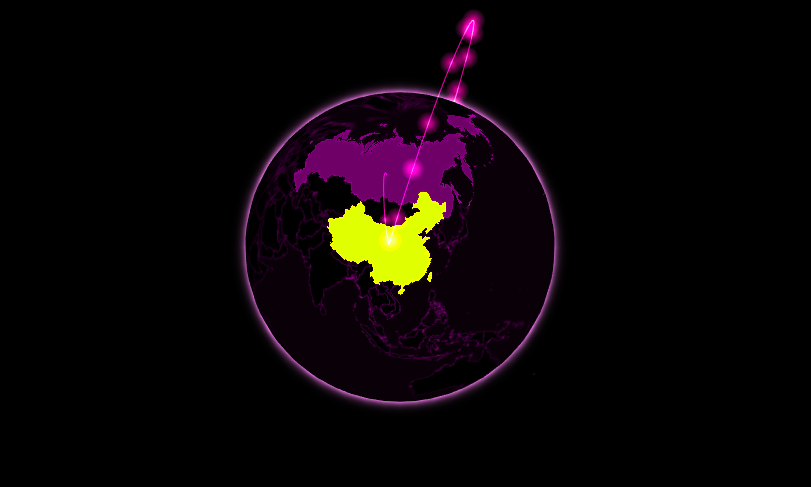
\includegraphics{images/gio-style.png}
\caption{Gio with a new style}
\end{figure}

This is great but can be greatly improved upon with the magrittr pipe \citep{R-magrittr}, it would allow easily passing the output of each function to the next to obtain an API akin to that of plotly or highcharter.

\begin{Shaded}
\begin{Highlighting}[]
\KeywordTok{library}\NormalTok{(magrittr)}

\KeywordTok{gio}\NormalTok{(arcs) }\OperatorTok{\%>\%}\StringTok{ }
\StringTok{  }\KeywordTok{gio\_style}\NormalTok{(}\StringTok{"juicyCake"}\NormalTok{)}
\end{Highlighting}
\end{Shaded}

The pipe drastically improves the API that gio provides its users and thus probably should be exported by the package; the usethis package provides a function to easily do so.

\begin{Shaded}
\begin{Highlighting}[]
\CommentTok{\# export the pipe}
\NormalTok{usethis}\OperatorTok{::}\KeywordTok{use\_pipe}\NormalTok{()}
\end{Highlighting}
\end{Shaded}

This closes this chapter but is not the last we see of gio.js, we shall use it as example in the next chapters as we extend its functionalities, polish certain aspects such as sizing and security.

\hypertarget{advanced-topics}{%
\chapter{Advanced Topics}\label{advanced-topics}}

In the previous chapter we put together an interesting, fully functioning widget but it lacks polish and does not use all the features htmlwidgets provides, this chapter explores those. We look into handling the size of widgets to ensure they are responsive as well as discuss potential security concerns and how to address them. Finally we show how to pass JavaScript code from R to JavaScript and how to add HTML content before and after the widget.

\hypertarget{shared-variables}{%
\section{Shared Variables}\label{shared-variables}}

Up until now the topic of shared variables had been omitted as it was not relevant, however, it will be from here onwards. Indeed we are about to discover how to further manipulate the widget; changing the data, resizing, and more. This will generally involve the JavaScript instance of the visualisation, the object named \texttt{controller} in the gio package, which, being defined in the \texttt{renderValue} function, is not accessible outside of it. To make it accessible outside of \texttt{renderValue} requires a tiny but consequential change without which resizing the widget will not be doable for instance.

The \texttt{controller} variable has to be declared outside of the \texttt{renderValue} function, inside the \texttt{factory}. This was in fact indicated from the onset by the following comment: \texttt{//\ TODO:\ define\ shared\ variables\ for\ this\ instance} (generated by \texttt{htmlwidgets::scaffoldWidget}). Any variable declared as shown below will be accessible by all functions declared in the \texttt{factory}; \texttt{renderValue}, but also \texttt{resize} and others yet to be added.

\begin{Shaded}
\begin{Highlighting}[]
\VariableTok{HTMLWidgets}\NormalTok{.}\AttributeTok{widget}\NormalTok{(}\OperatorTok{\{}

  \DataTypeTok{name}\OperatorTok{:} \StringTok{\textquotesingle{}gio\textquotesingle{}}\OperatorTok{,}

  \DataTypeTok{type}\OperatorTok{:} \StringTok{\textquotesingle{}output\textquotesingle{}}\OperatorTok{,}

  \DataTypeTok{factory}\OperatorTok{:} \KeywordTok{function}\NormalTok{(el}\OperatorTok{,}\NormalTok{ width}\OperatorTok{,}\NormalTok{ height) }\OperatorTok{\{}

    \CommentTok{// }\AlertTok{TODO}\CommentTok{: define shared variables for this instance}
    \KeywordTok{var}\NormalTok{ controller}\OperatorTok{;}

    \ControlFlowTok{return} \OperatorTok{\{}

      \DataTypeTok{renderValue}\OperatorTok{:} \KeywordTok{function}\NormalTok{(x) }\OperatorTok{\{}

\NormalTok{        controller }\OperatorTok{=} \KeywordTok{new} \VariableTok{GIO}\NormalTok{.}\AttributeTok{Controller}\NormalTok{(el)}\OperatorTok{;} \CommentTok{// declared outside}
        
        \CommentTok{// add data}
        \VariableTok{controller}\NormalTok{.}\AttributeTok{addData}\NormalTok{(}\VariableTok{x}\NormalTok{.}\AttributeTok{data}\NormalTok{)}\OperatorTok{;}

        \CommentTok{// define style}
        \VariableTok{controller}\NormalTok{.}\AttributeTok{setStyle}\NormalTok{(}\VariableTok{x}\NormalTok{.}\AttributeTok{style}\NormalTok{)}\OperatorTok{;}

        \CommentTok{// render}
        \VariableTok{controller}\NormalTok{.}\AttributeTok{init}\NormalTok{()}\OperatorTok{;}

      \OperatorTok{\},}

      \DataTypeTok{resize}\OperatorTok{:} \KeywordTok{function}\NormalTok{(width}\OperatorTok{,}\NormalTok{ height) }\OperatorTok{\{}

        \CommentTok{// }\AlertTok{TODO}\CommentTok{: code to re{-}render the widget with a new size}

      \OperatorTok{\}}

    \OperatorTok{\};}
  \OperatorTok{\}}
\OperatorTok{\}}\NormalTok{)}\OperatorTok{;}
\end{Highlighting}
\end{Shaded}

\hypertarget{sizing}{%
\subsection{Sizing}\label{sizing}}

The \texttt{gio} function of the package we developed in the previous chapter has arguments to specify the dimensions of the visualisation (width and height). However, think how rarely (if ever) one specifies these parameters when using plotly, highcharter or leaflet. Indeed HTML visualisations should be responsive and fit the container they are placed in---not to be confused though, these are two different things. This enables creating visualisations that look great on large desktop screens as well as the smaller mobile phones or iPad screens. Pre-defining the dimensions of the visualisation (e.g.: \texttt{400px}), breaks all responsiveness as the width is no longer relative to its container. Using a relative width like \texttt{100\%} ensures the visualisation always fits in the container edge to edge and enables responsiveness.

\begin{Shaded}
\begin{Highlighting}[]
\NormalTok{arcs <{-}}\StringTok{ }\NormalTok{jsonlite}\OperatorTok{::}\KeywordTok{fromJSON}\NormalTok{(}
  \StringTok{\textquotesingle{}[}
\StringTok{    \{}
\StringTok{      "e": "CN",}
\StringTok{      "i": "US",}
\StringTok{      "v": 3300000}
\StringTok{    \},}
\StringTok{    \{}
\StringTok{      "e": "CN",}
\StringTok{      "i": "RU",}
\StringTok{      "v": 10000}
\StringTok{    \}}
\StringTok{  ]\textquotesingle{}}
\NormalTok{)}

\KeywordTok{gio}\NormalTok{(arcs)}
\end{Highlighting}
\end{Shaded}

\begin{figure}
\centering
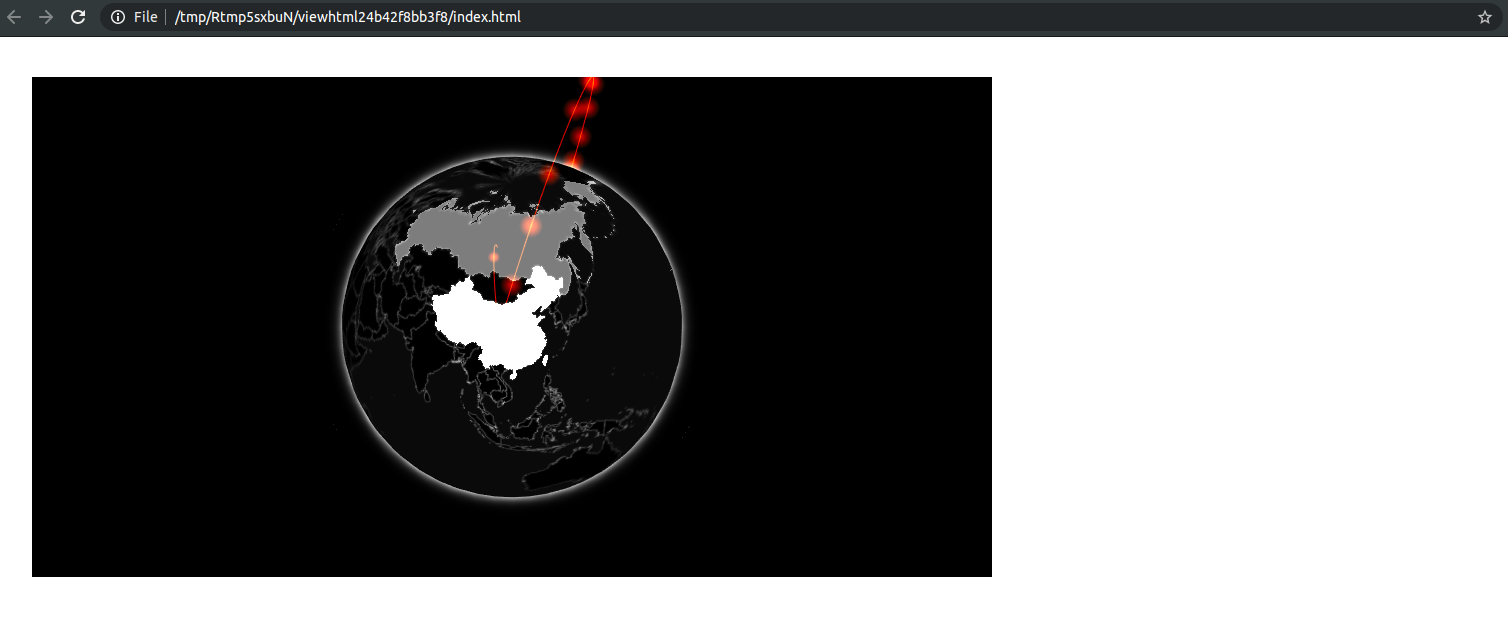
\includegraphics{images/gio-size-issue.png}
\caption{Gio with no sizing management}
\end{figure}

When this is not specified htmlwidgets sets the width of the visualisation to 400 pixels.

\begin{Shaded}
\begin{Highlighting}[]
\KeywordTok{gio}\NormalTok{(arcs, }\DataTypeTok{width =} \DecValTok{500}\NormalTok{) }\CommentTok{\# 500 pixels wide}
\KeywordTok{gio}\NormalTok{(arcs, }\DataTypeTok{width =} \StringTok{"100\%"}\NormalTok{) }\CommentTok{\# fits width}
\end{Highlighting}
\end{Shaded}

These options are destined for the user of the package, the next section details how the developer can define default sizing behaviour.

\hypertarget{sizing-policy}{%
\subsection{Sizing Policy}\label{sizing-policy}}

One can specify a sizing policy when creating the widget, the sizing policy will dictate default dimensions and padding given different contexts:

\begin{itemize}
\tightlist
\item
  Global defaults
\item
  RStudio viewer
\item
  Web browser
\item
  R markdown
\end{itemize}

It is often enough to specify general defaults as widgets are rarely expected to behave differently with respect to size depending on the context but it can be useful in some cases.

Below we modify the sizing policy of gio via the \texttt{sizingPolicy} argument of the \texttt{createWidget} function. The function \texttt{htmlwidgets::sizingPolicy} has many arguments, we set the default width to 100\% to ensure the visualisation fills its container entirely regardless of where it is rendered. We also remove all padding by setting it to 0 and set \texttt{browser.fill} to \texttt{TRUE} so it automatically resizes the visualisation to fit the entire browser page.

\begin{Shaded}
\begin{Highlighting}[]
\CommentTok{\# create widget}
\NormalTok{htmlwidgets}\OperatorTok{::}\KeywordTok{createWidget}\NormalTok{(}
  \DataTypeTok{name =} \StringTok{\textquotesingle{}gio\textquotesingle{}}\NormalTok{,}
\NormalTok{  x,}
  \DataTypeTok{width =}\NormalTok{ width,}
  \DataTypeTok{height =}\NormalTok{ height,}
  \DataTypeTok{package =} \StringTok{\textquotesingle{}gio\textquotesingle{}}\NormalTok{,}
  \DataTypeTok{elementId =}\NormalTok{ elementId,}
  \DataTypeTok{sizingPolicy =}\NormalTok{ htmlwidgets}\OperatorTok{::}\KeywordTok{sizingPolicy}\NormalTok{(}
    \DataTypeTok{defaultWidth =} \StringTok{"100\%"}\NormalTok{,}
    \DataTypeTok{padding =} \DecValTok{0}\NormalTok{,}
    \DataTypeTok{browser.fill =} \OtherTok{TRUE}
\NormalTok{  )}
\NormalTok{)}
\end{Highlighting}
\end{Shaded}

\begin{figure}
\centering
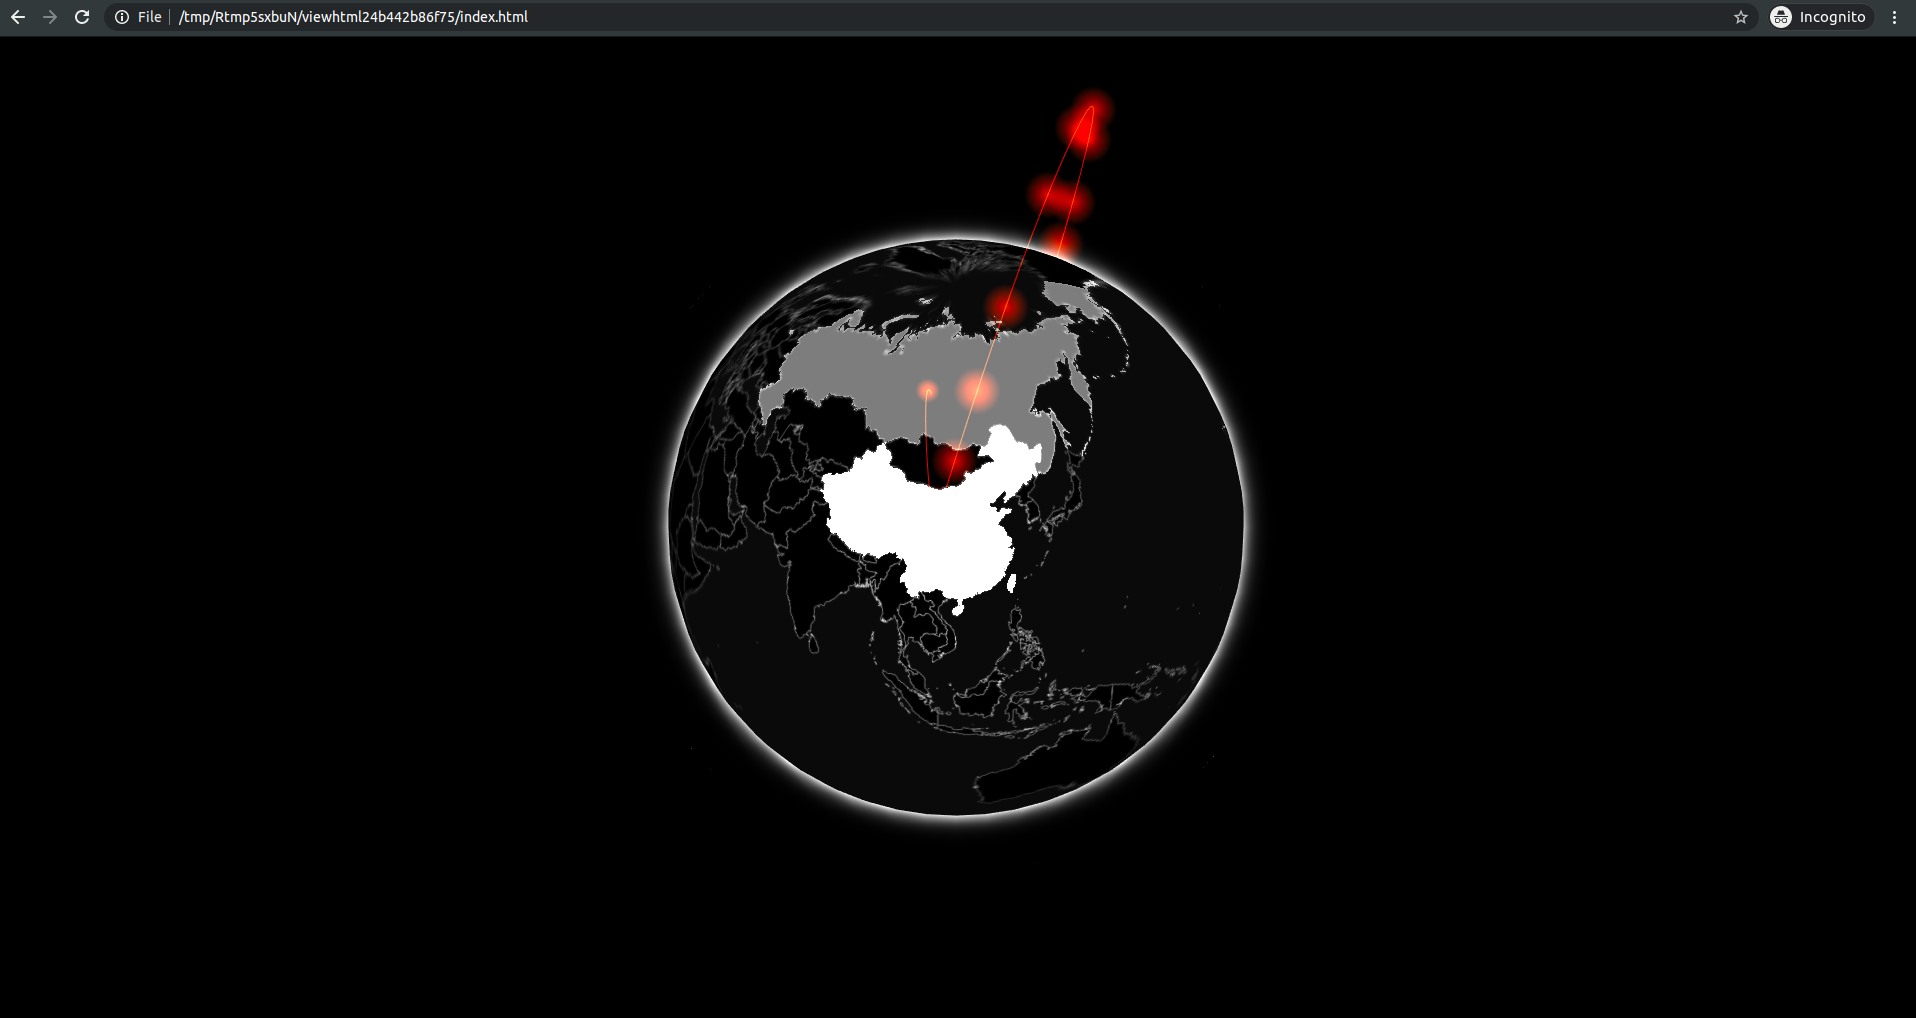
\includegraphics{images/gio-fit.png}
\caption{Gio with sizing policy}
\end{figure}

\hypertarget{resizing}{%
\section{Resizing}\label{resizing}}

In the first widget built in this book (\texttt{playground}), when we deconstructed the JavaScript \texttt{factory} function but omitted the \texttt{resize} function. The \texttt{resize} function does what it says on the tin: it is called when the widget is resized. What this function will contain entirely depends on the JavaScript library one is working with. Some are very easy to resize other less so, that is for the developer to discover in the documentation of the library. Some libraries, like gio, do not even require using a resizing function and handle that automatically under the hood; resize the width of the RStudio viewer or web browser and gio.js resizes too. This said, there is a function to force resize gio, though it is not in the official documentation it can be found in the source code: \texttt{resizeUpdate} is a method of the controller and does not take any argument.

\begin{Shaded}
\begin{Highlighting}[]
\NormalTok{...}
\NormalTok{resize}\OperatorTok{:} \KeywordTok{function}\NormalTok{(width}\OperatorTok{,}\NormalTok{ height) }\OperatorTok{\{}
  \VariableTok{controller}\NormalTok{.}\AttributeTok{resizeUpdate}\NormalTok{()}\OperatorTok{;}
\OperatorTok{\}}
\NormalTok{...}
\end{Highlighting}
\end{Shaded}

\begin{figure}
\centering
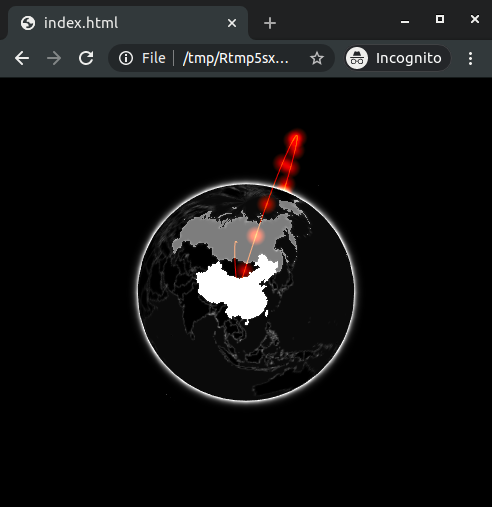
\includegraphics{images/gio-small.png}
\caption{Gio resized}
\end{figure}

To give the reader a better idea of what these tend to look like below are the ways plotly, highcharts, and chart.js do it.

\textbf{Plotly}

\begin{Shaded}
\begin{Highlighting}[]
\VariableTok{Plotly}\NormalTok{.}\AttributeTok{relayout}\NormalTok{(}\StringTok{\textquotesingle{}chartid\textquotesingle{}}\OperatorTok{,} \OperatorTok{\{}\DataTypeTok{width}\OperatorTok{:}\NormalTok{ width}\OperatorTok{,} \DataTypeTok{height}\OperatorTok{:}\NormalTok{ height}\OperatorTok{\}}\NormalTok{)}\OperatorTok{;}
\end{Highlighting}
\end{Shaded}

\textbf{Highcharts}

\begin{Shaded}
\begin{Highlighting}[]
\VariableTok{chart}\NormalTok{.}\AttributeTok{setSize}\NormalTok{(width}\OperatorTok{,}\NormalTok{ height)}\OperatorTok{;}
\end{Highlighting}
\end{Shaded}

\textbf{Chart.js}

\begin{Shaded}
\begin{Highlighting}[]
\VariableTok{chart}\NormalTok{.}\AttributeTok{resize}\NormalTok{()}\OperatorTok{;}
\end{Highlighting}
\end{Shaded}

Note that the \texttt{width} and \texttt{height} used in the functions above are obtained from the \texttt{resize} function itself (see arguments).

That is one of the reasons for ensuring the instance of the visualisation (\texttt{controller} in this case) is shared (declared in \texttt{factory}), if declared in the \texttt{renderValue} function then the \texttt{resize} function cannot access that object and thus cannot run the function required to resize the widget.

\hypertarget{pre-render-hooks-security}{%
\section{Pre Render Hooks \& Security}\label{pre-render-hooks-security}}

The \texttt{createWidget} function also comes with a \texttt{preRenderHook} argument which accepts a function that is run just prior to the rendering, this function should accept the entire widget object as input, and should return a modified widget object. This was not used in any of the widgets previously built but is extremely useful. It can be used to make checks on the object to ensure all is correct, or remove variables that should only be used internally, and much more.

Currently, \texttt{gio} takes the data frame \texttt{data} and serialises it in its entirety which will cause security concerns as all the data used in the widget is visible in the source code of the output. What if the data used for the visualisation contained an additional column with sensitive information? We ought to ensure gio only serialises the data necessary to produce the visualisation.

\begin{Shaded}
\begin{Highlighting}[]
\CommentTok{\# add a variable that should not be shared}
\NormalTok{arcs}\OperatorTok{$}\NormalTok{secret\_id <{-}}\StringTok{ }\DecValTok{1}\OperatorTok{:}\DecValTok{2}
\end{Highlighting}
\end{Shaded}

We create a \texttt{render\_gio} function which accepts the entire widget, filters only the column necessary from the data and returns the widget. This function is then passed to the argument \texttt{preRenderHook} of the \texttt{htmlwidgets::createWidget} call. This way, only the columns \texttt{e}, \texttt{v}, and \texttt{i} of the data are kept thus the \texttt{secret\_id} column will not be exposed publicly.

\begin{Shaded}
\begin{Highlighting}[]
\CommentTok{\# preRenderHook function}
\NormalTok{render\_gio <{-}}\StringTok{ }\ControlFlowTok{function}\NormalTok{(g)\{}
  \CommentTok{\# only keep relevant variables}
\NormalTok{  g}\OperatorTok{$}\NormalTok{x}\OperatorTok{$}\NormalTok{data <{-}}\StringTok{ }\NormalTok{g}\OperatorTok{$}\NormalTok{x}\OperatorTok{$}\NormalTok{data[,}\KeywordTok{c}\NormalTok{(}\StringTok{"e"}\NormalTok{, }\StringTok{"v"}\NormalTok{, }\StringTok{"i"}\NormalTok{)]}
  \KeywordTok{return}\NormalTok{(g)}
\NormalTok{\}}

\CommentTok{\# create widget}
\NormalTok{htmlwidgets}\OperatorTok{::}\KeywordTok{createWidget}\NormalTok{(}
  \DataTypeTok{name =} \StringTok{\textquotesingle{}gio\textquotesingle{}}\NormalTok{,}
\NormalTok{  x,}
  \DataTypeTok{width =}\NormalTok{ width,}
  \DataTypeTok{height =}\NormalTok{ height,}
  \DataTypeTok{package =} \StringTok{\textquotesingle{}gio\textquotesingle{}}\NormalTok{,}
  \DataTypeTok{elementId =}\NormalTok{ elementId,}
  \DataTypeTok{sizingPolicy =}\NormalTok{ htmlwidgets}\OperatorTok{::}\KeywordTok{sizingPolicy}\NormalTok{(}
    \DataTypeTok{defaultWidth =} \StringTok{"100\%"}\NormalTok{,}
    \DataTypeTok{padding =} \DecValTok{0}\NormalTok{,}
    \DataTypeTok{browser.fill =} \OtherTok{TRUE}
\NormalTok{  ),}
  \DataTypeTok{preRenderHook =}\NormalTok{ render\_gio }\CommentTok{\# pass renderer}
\NormalTok{)}
\end{Highlighting}
\end{Shaded}

Moreover, security aside, this can also improve performances as only the data relevant to the visualisation is serialised and subsequently loaded by the client. Without the modification above, were one to use \texttt{gio} on a dataset with 100 columns all would have been serialised, thereby greatly impacting performances both of the R process rendering the output and the web browser viewing the visualisation.

\hypertarget{javascript-code}{%
\section{JavaScript Code}\label{javascript-code}}

As mentioned in a previous chapter JavaScript code cannot be serialised to JSON.

\begin{Shaded}
\begin{Highlighting}[]
\CommentTok{\# serialised as string}
\NormalTok{jsonlite}\OperatorTok{::}\KeywordTok{toJSON}\NormalTok{(}\StringTok{"var x = 3;"}\NormalTok{)}
\end{Highlighting}
\end{Shaded}

\begin{verbatim}
## ["var x = 3;"]
\end{verbatim}

Nonetheless, it is doable with htmlwidgets' serialiser (and only that one). The function \texttt{htmlwidgets::JS} can be used to mark a character vector so that it will be treated as JavaScript code when evaluated in the browser.

\begin{Shaded}
\begin{Highlighting}[]
\NormalTok{htmlwidgets}\OperatorTok{::}\KeywordTok{JS}\NormalTok{(}\StringTok{"var x = 3;"}\NormalTok{)  }
\end{Highlighting}
\end{Shaded}

\begin{verbatim}
## [1] "var x = 3;"
## attr(,"class")
## [1] "JS_EVAL"
\end{verbatim}

This can be useful where the library requires the use of callback functions for instance.

\begin{rmdnote}
Replacing the serialiser will break this feature.
\end{rmdnote}

\hypertarget{prepend-append-content}{%
\section{Prepend \& Append Content}\label{prepend-append-content}}

There is the ability to append of prepend HTML content to the widget (shiny, htmltools tags, or a list of those). For instance, we could use \texttt{htmlwidgets::prependContent} to allow displaying a title to the visualisation as shown below.

\begin{Shaded}
\begin{Highlighting}[]
\CommentTok{\#\textquotesingle{} @export}
\NormalTok{gio\_title <{-}}\StringTok{ }\ControlFlowTok{function}\NormalTok{(g, title)\{}
\NormalTok{  title <{-}}\StringTok{ }\NormalTok{htmltools}\OperatorTok{::}\KeywordTok{h3}\NormalTok{(title)}
\NormalTok{  htmlwidgets}\OperatorTok{::}\KeywordTok{prependContent}\NormalTok{(g, title)}
\NormalTok{\}}
\end{Highlighting}
\end{Shaded}

\begin{Shaded}
\begin{Highlighting}[]
\KeywordTok{gio}\NormalTok{(arcs) }\OperatorTok{\%>\%}\StringTok{ }
\StringTok{  }\KeywordTok{gio\_title}\NormalTok{(}\StringTok{"Gio.js htmlwidget!"}\NormalTok{)}
\end{Highlighting}
\end{Shaded}

\begin{figure}
\centering
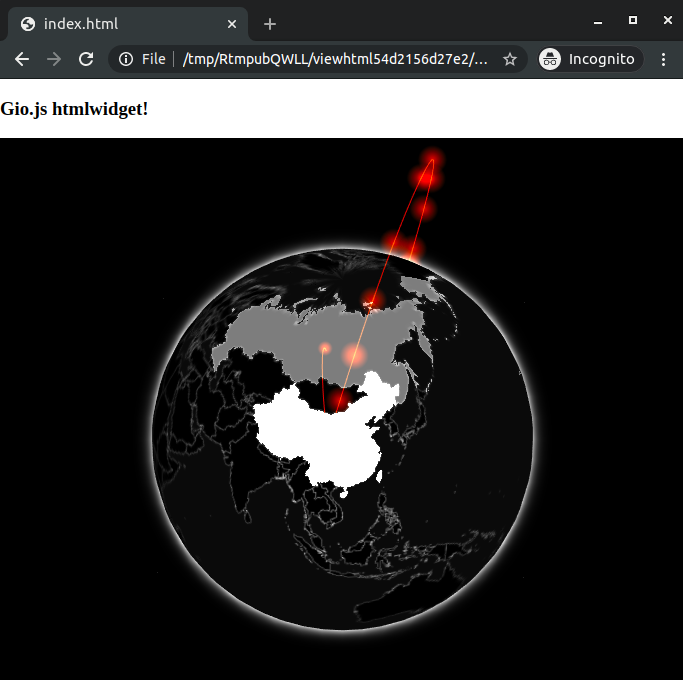
\includegraphics{images/gio-title.png}
\caption{Gio output with a title}
\end{figure}

While the \texttt{prependContent} function places the content above the visualisation, the \texttt{appendContent} function places it below, as they accept any valid htmltools or shiny tag they can also be used for conditional CSS styling for instance.

\begin{rmdnote}
\texttt{prependContent} and \texttt{appendContent} do not work in shiny.
\end{rmdnote}

\hypertarget{dependencies}{%
\section{Dependencies}\label{dependencies}}

Thus far, this book has only covered one of two ways dependencies can be included in htmlwidgets. Though the one covered, using the \texttt{.yml} file, will likely be necessary for every widget it has one drawback: all dependencies listed in the file are always included with the output. Dependencies can greatly affect the load time of the output (be it a standalone visualisation, an R markdown document, or a shiny application) as these files may be large. Most large visualisation libraries will therefore allow to bundle those dependencies in separate files. For instance, ECharts.js provides a way to customise the bundle to only include dependencies for charts that one wants to draw (e.g.: bar chart, or boxplot), Highcharts also allows splitting dependencies so one can load those needed for maps, stock charts, and more, separately. It is thus good practice to do the same in widgets so only the required dependencies are loaded, e.g.: when the user produces a map, only the dependency for that map is loaded. It is used in the leaflet package to load map tiles for instance.

The Google Chrome network tab shows information on resources downloaded by the browser (including dependencies) including how long it takes. It is advisable to take a look at it to ensure no dependency drags load time.

\begin{figure}
\centering
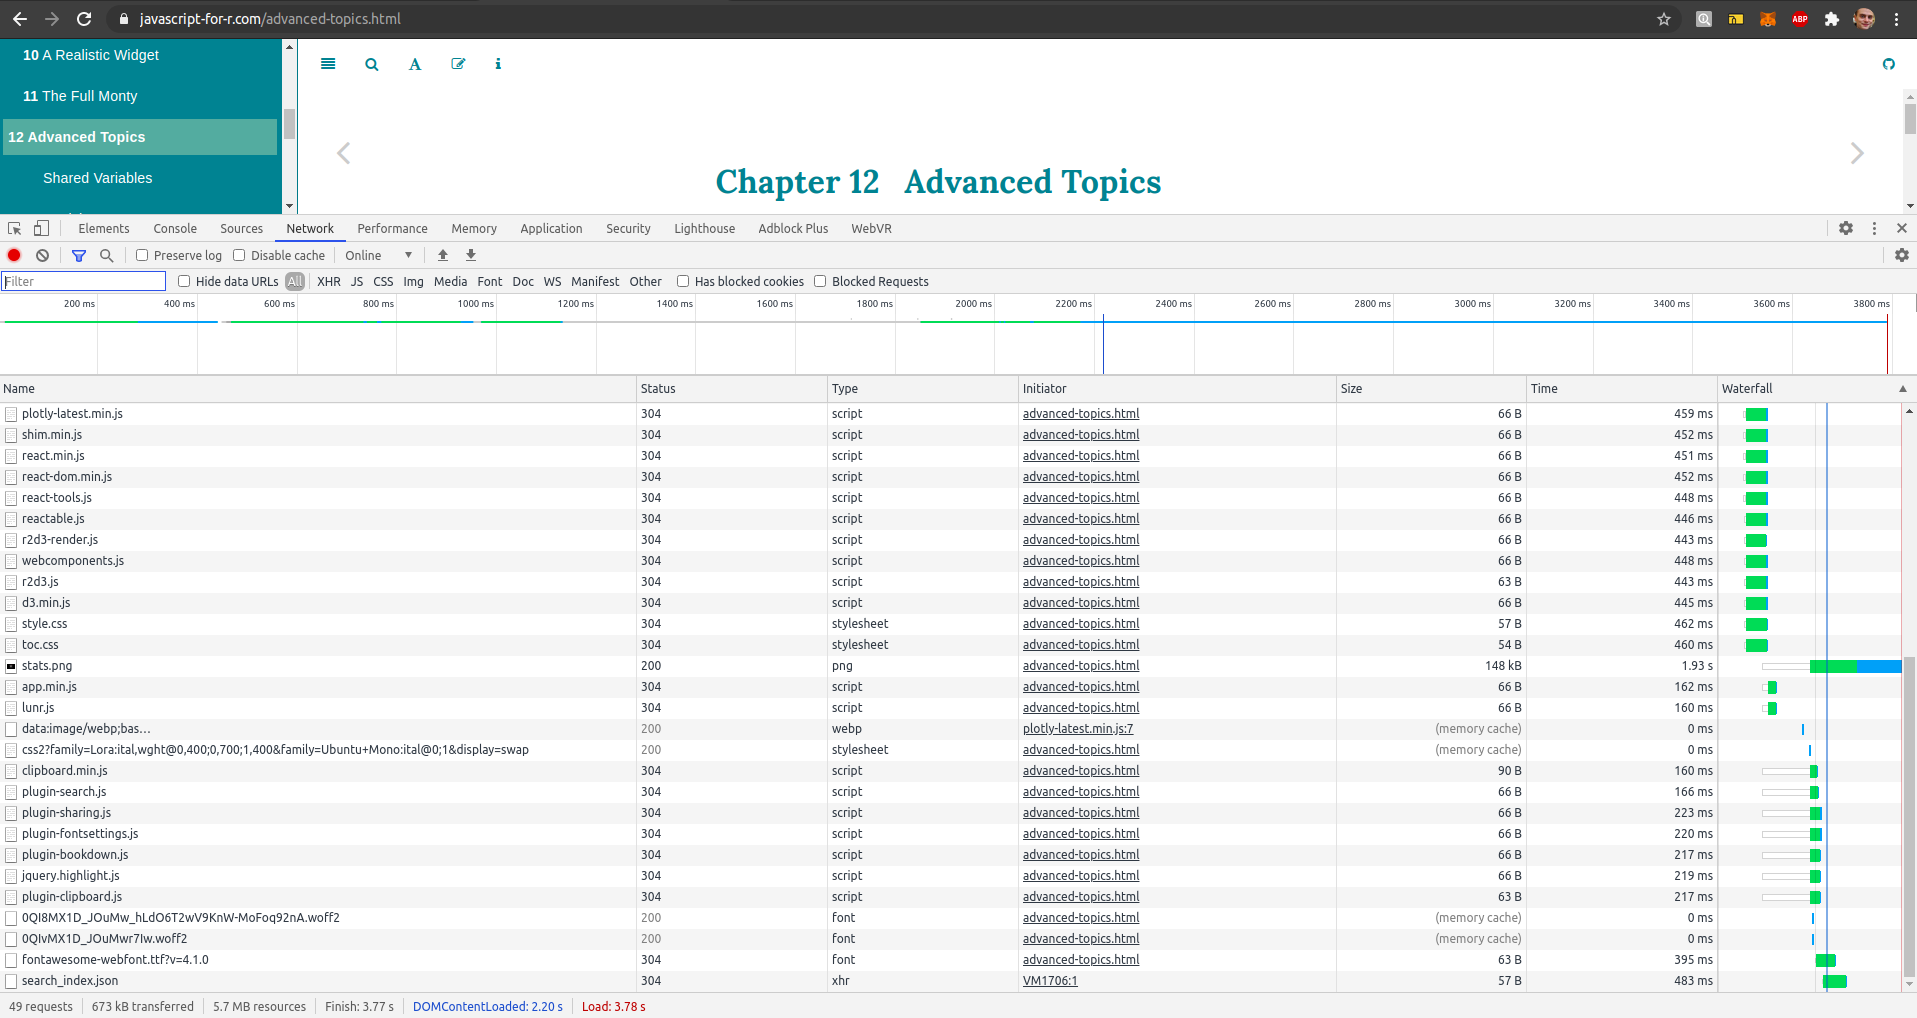
\includegraphics{images/htmlwidgets-performances.png}
\caption{Google Chrome network tab}
\end{figure}

To demonstrate, we will add a function in gio to optionally include \href{https://github.com/mrdoob/stats.js/}{stats.js}, a JavaScript performance monitor which displays information such as the number of frames per second (FPS) rendered, or the number of milliseconds needed to render the visualisation. Gio.js natively supports stats.js but the dependency needs to be imported and that option needs to be enabled on the \texttt{controller} as shown in the \href{https://giojs.org/html/docs/interfaceStats.html}{documentation}.

\begin{Shaded}
\begin{Highlighting}[]
\CommentTok{// enable stats}
\VariableTok{controller}\NormalTok{.}\AttributeTok{enableStats}\NormalTok{()}\OperatorTok{;}
\end{Highlighting}
\end{Shaded}

In htmlwidgets those additional dependencies can be specified via the \texttt{dependencies} argument in the \texttt{htmlwidgets::createWidget} function, or they can be appended to the output of that function.

\begin{verbatim}
# create gio object
g <- gio::gio(arcs)

is.null(g$dependencies)
\end{verbatim}

\begin{verbatim}
[1] TRUE
\end{verbatim}

As shown above, the object created by \texttt{gio} includes dependencies, currently \texttt{NULL} as no such extra dependency is specified. One can therefore append those to that object in a fashion similar to what the \texttt{gio\_style} function does.

From the root of the gio package we create a new directory for the stats.js dependency and download version \texttt{r17} from the CDN.

\begin{Shaded}
\begin{Highlighting}[]
\KeywordTok{dir.create}\NormalTok{(}\StringTok{"htmlwidgets/stats"}\NormalTok{)}
\NormalTok{url <{-}}\StringTok{ }\KeywordTok{paste0}\NormalTok{(}
  \StringTok{"https://cdnjs.cloudflare.com/ajax/libs/"}\NormalTok{,}
  \StringTok{"stats.js/r17/Stats.min.js"}
\NormalTok{)}
\KeywordTok{download.file}\NormalTok{(url, }\DataTypeTok{destfile =} \StringTok{"htmlwidgets/stats/stats.min.js"}\NormalTok{)}
\end{Highlighting}
\end{Shaded}

First we use the \texttt{system.file} function to retrieve \emph{the path to the directory} which contains the dependency (\texttt{stats.min.js}). It's important that it is the path to the directory and not the file itself.

\begin{Shaded}
\begin{Highlighting}[]
\CommentTok{\# stats.R}
\NormalTok{gio\_stats <{-}}\StringTok{ }\ControlFlowTok{function}\NormalTok{(g)\{}

  \CommentTok{\# create dependency}
\NormalTok{  path <{-}}\StringTok{ }\KeywordTok{system.file}\NormalTok{(}\StringTok{"htmlwidgets/stats"}\NormalTok{, }\DataTypeTok{package =} \StringTok{"gio"}\NormalTok{)}

  \KeywordTok{return}\NormalTok{(g)}

\NormalTok{\}}
\end{Highlighting}
\end{Shaded}

Then we use the htmltools package to create a dependency, the \texttt{htmltools::htmlDependency} function returns an object of class \texttt{html\_dependency} which htmlwidgets can understand and subsequently insert in the output. On the \texttt{src} parameter, since we reference a dependency from the filesystem we name the character string \texttt{file} but we could use the CDN (web hosted file) and name it \texttt{href} instead.

\begin{Shaded}
\begin{Highlighting}[]
\CommentTok{\# stats.R}
\NormalTok{gio\_stats <{-}}\StringTok{ }\ControlFlowTok{function}\NormalTok{(g)\{}

  \CommentTok{\# create dependency}
\NormalTok{  path <{-}}\StringTok{ }\KeywordTok{system.file}\NormalTok{(}\StringTok{"htmlwidgets/stats"}\NormalTok{, }\DataTypeTok{package =} \StringTok{"gio"}\NormalTok{)}
\NormalTok{  dep <{-}}\StringTok{ }\NormalTok{htmltools}\OperatorTok{::}\KeywordTok{htmlDependency}\NormalTok{(}
    \DataTypeTok{name =} \StringTok{"stats"}\NormalTok{,}
    \DataTypeTok{version =} \StringTok{"17"}\NormalTok{,}
    \DataTypeTok{src =} \KeywordTok{c}\NormalTok{(}\DataTypeTok{file =}\NormalTok{ path),}
    \DataTypeTok{script =} \StringTok{"stats.min.js"}
\NormalTok{  )}

  \KeywordTok{return}\NormalTok{(g)}

\NormalTok{\}}
\end{Highlighting}
\end{Shaded}

The dependency then needs to be appended to the htmlwidgets object.

\begin{Shaded}
\begin{Highlighting}[]
\CommentTok{\# stats.R}
\NormalTok{gio\_stats <{-}}\StringTok{ }\ControlFlowTok{function}\NormalTok{(g)\{}

  \CommentTok{\# create dependency}
\NormalTok{  path <{-}}\StringTok{ }\KeywordTok{system.file}\NormalTok{(}\StringTok{"htmlwidgets/stats"}\NormalTok{, }\DataTypeTok{package =} \StringTok{"gio"}\NormalTok{)}
\NormalTok{  dep <{-}}\StringTok{ }\NormalTok{htmltools}\OperatorTok{::}\KeywordTok{htmlDependency}\NormalTok{(}
    \DataTypeTok{name =} \StringTok{"stats"}\NormalTok{,}
    \DataTypeTok{version =} \StringTok{"17"}\NormalTok{,}
    \DataTypeTok{src =} \KeywordTok{c}\NormalTok{(}\DataTypeTok{file =}\NormalTok{ path),}
    \DataTypeTok{script =} \StringTok{"stats.min.js"}
\NormalTok{  )}

  \CommentTok{\# append dependency}
\NormalTok{  g}\OperatorTok{$}\NormalTok{dependencies <{-}}\StringTok{ }\KeywordTok{append}\NormalTok{(g}\OperatorTok{$}\NormalTok{dependencies, }\KeywordTok{list}\NormalTok{(dep))}

  \KeywordTok{return}\NormalTok{(g)}

\NormalTok{\}}
\end{Highlighting}
\end{Shaded}

Finally, we pass an additional variable in the list of options (\texttt{x}) which we will use JavaScript-side to check whether stats.js must be enabled.

\begin{Shaded}
\begin{Highlighting}[]
\CommentTok{\#\textquotesingle{} @export}
\NormalTok{gio\_stats <{-}}\StringTok{ }\ControlFlowTok{function}\NormalTok{(g)\{}

  \CommentTok{\# create dependency}
\NormalTok{  path <{-}}\StringTok{ }\KeywordTok{system.file}\NormalTok{(}\StringTok{"htmlwidgets/stats"}\NormalTok{, }\DataTypeTok{package =} \StringTok{"gio"}\NormalTok{)}
\NormalTok{  dep <{-}}\StringTok{ }\NormalTok{htmltools}\OperatorTok{::}\KeywordTok{htmlDependency}\NormalTok{(}
    \DataTypeTok{name =} \StringTok{"stats"}\NormalTok{,}
    \DataTypeTok{version =} \StringTok{"17"}\NormalTok{,}
    \DataTypeTok{src =} \KeywordTok{c}\NormalTok{(}\DataTypeTok{file =}\NormalTok{ path),}
    \DataTypeTok{script =} \StringTok{"stats.min.js"}
\NormalTok{  )}

  \CommentTok{\# append dependency to gio.js}
\NormalTok{  g}\OperatorTok{$}\NormalTok{dependencies <{-}}\StringTok{ }\KeywordTok{append}\NormalTok{(g}\OperatorTok{$}\NormalTok{dependencies, }\KeywordTok{list}\NormalTok{(dep))}

  \CommentTok{\# add stats variable}
\NormalTok{  g}\OperatorTok{$}\NormalTok{x}\OperatorTok{$}\NormalTok{stats <{-}}\StringTok{ }\OtherTok{TRUE}

  \KeywordTok{return}\NormalTok{(g)}
\NormalTok{\}}
\end{Highlighting}
\end{Shaded}

Then it's a matter of using the \texttt{stats} variable added to \texttt{x} in the JavaScript \texttt{renderValue} function to determine whether the stats feature should be enabled.

\begin{Shaded}
\begin{Highlighting}[]
\CommentTok{// gio.js}
\ControlFlowTok{if}\NormalTok{(}\VariableTok{x}\NormalTok{.}\AttributeTok{stats}\NormalTok{)}
  \VariableTok{controller}\NormalTok{.}\AttributeTok{enableStats}\NormalTok{()}\OperatorTok{;}

\VariableTok{controller}\NormalTok{.}\AttributeTok{init}\NormalTok{()}\OperatorTok{;}
\end{Highlighting}
\end{Shaded}

Then the package can be documented to export the newly created function and loaded in the environment to test the feature.

\begin{Shaded}
\begin{Highlighting}[]
\CommentTok{\# create gio object}
\NormalTok{arcs }\OperatorTok{\%>\%}\StringTok{ }
\StringTok{  }\KeywordTok{gio}\NormalTok{() }\OperatorTok{\%>\%}\StringTok{ }
\StringTok{  }\KeywordTok{gio\_stats}\NormalTok{()}
\end{Highlighting}
\end{Shaded}

\begin{figure}
\centering
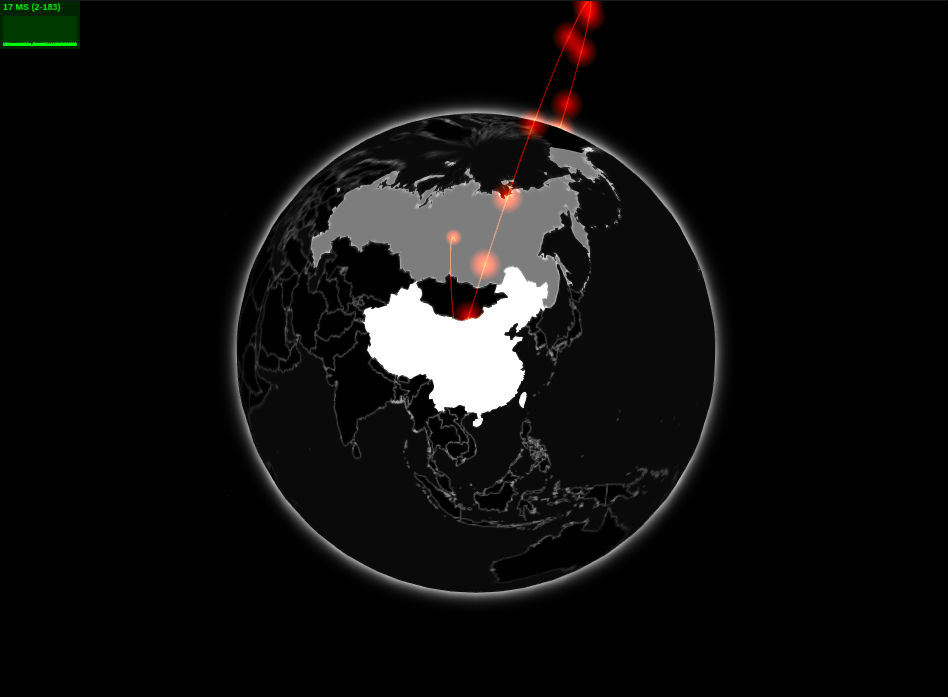
\includegraphics{images/stats.png}
\caption{Gio with stats output}
\end{figure}

In brief, it is better to only place the hard dependencies in the \texttt{.yml} file; dependencies that are absolutely necessary to producing the visualisation and use dynamic dependencies where ever possible. Perhaps one can think of it as the difference between \texttt{Imports} and \texttt{Suggests} in an R package \texttt{DESCRIPTION} file.

\hypertarget{compatibility}{%
\section{Compatibility}\label{compatibility}}

One issue that might arise is that of compatibility between widgets. What if someone else builds another htmlwidget for gio.js which uses a different version of the library and that a user decides to use both packages in a shiny app or R markdown document? Something is likely to fail as two different version of gio.js are imported and that one overrides the other. For instance, the package echarts4r \citep{R-echarts4r} allows working with leaflet but including the dependencies could clash with the leaflet package itself, therefore it uses the dependencies from the leaflet package instead.

The htmlwidgets package comes with a function to extract the dependencies from a widget, so they can be reused in another. The function \texttt{htmlwidgets::getDependency} returns a list of objects of class \texttt{html\_dependency} which can therefore be used in other widgets as demonstrated in the previous section.

\begin{Shaded}
\begin{Highlighting}[]
\CommentTok{\# get dependencies of the gio package}
\NormalTok{htmlwidgets}\OperatorTok{::}\KeywordTok{getDependency}\NormalTok{(}\StringTok{"gio"}\NormalTok{)[}\DecValTok{2}\OperatorTok{:}\DecValTok{3}\NormalTok{]}
\end{Highlighting}
\end{Shaded}

\begin{verbatim}
## [[1]]
## List of 10
##  $ name      : chr "three"
##  $ version   : chr "110"
##  $ src       :List of 1
##   ..$ file: chr "/home/jp/R/x86_64-pc-linux-gnu-library/4.0/gio/htmlwidgets/three"
##  $ meta      : NULL
##  $ script    : chr "three.min.js"
##  $ stylesheet: NULL
##  $ head      : NULL
##  $ attachment: NULL
##  $ package   : NULL
##  $ all_files : logi TRUE
##  - attr(*, "class")= chr "html_dependency"
## 
## [[2]]
## List of 10
##  $ name      : chr "gio"
##  $ version   : chr "2"
##  $ src       :List of 1
##   ..$ file: chr "/home/jp/R/x86_64-pc-linux-gnu-library/4.0/gio/htmlwidgets/gio"
##  $ meta      : NULL
##  $ script    : chr "gio.min.js"
##  $ stylesheet: NULL
##  $ head      : NULL
##  $ attachment: NULL
##  $ package   : NULL
##  $ all_files : logi TRUE
##  - attr(*, "class")= chr "html_dependency"
\end{verbatim}

\hypertarget{unit-tests}{%
\section{Unit Tests}\label{unit-tests}}

The best way to write unit tests for htmlwidgets is to test the object created by \texttt{htmlwidgets::createWidget}. Below we provide an example using testthat\citep{R-testthat}, running \texttt{expect*} functions on the output of \texttt{gio}.

\begin{Shaded}
\begin{Highlighting}[]
\KeywordTok{library}\NormalTok{(gio)}
\KeywordTok{library}\NormalTok{(testthat)}

\KeywordTok{test\_that}\NormalTok{(}\StringTok{"gio has correct data"}\NormalTok{, \{}
\NormalTok{  g <{-}}\StringTok{ }\KeywordTok{gio}\NormalTok{(arcs)}

  \CommentTok{\# internally stored as data.frame}
  \KeywordTok{expect\_is}\NormalTok{(g}\OperatorTok{$}\NormalTok{x}\OperatorTok{$}\NormalTok{data, }\StringTok{"data.frame"}\NormalTok{)}

  \CommentTok{\# gio does not work without data}
  \KeywordTok{expect\_error}\NormalTok{(}\KeywordTok{gio}\NormalTok{())}
\NormalTok{\})}
\end{Highlighting}
\end{Shaded}

\hypertarget{performances}{%
\section{Performances}\label{performances}}

A few hints have already been given to ensure one does not drain the browser, consider assessing the performances of the widget as it is being built. Always try and imagine what happens under the hood of the htmlwidget as you build it, it often reveals potential bottlenecks and solutions.

Remember that data passed to \texttt{htmlwidgets::createWidget} is 1) loaded into R, 2) serialised to JSON, 3) embedded into the HTML output, 4) read back in with JavaScript, which adds some overhead considering it might be read into JavaScript directly. This will not be a problem for most visualisations but might become one when that data is large. Indeed, there are sometimes more efficient ways to load data into web browsers where it is needed for the visualisation.

Consider for instance geographic features (topoJSON and GeoJSON), why load them into R if it is to then re-serialise it to JSON?

Also keep the previous remark in mind when repeatedly serialising identical data objects, GeoJSON is again a good example. A map used twice or more should only be serialised once or better not at all. Consider providing other ways to for the developer to make potentially large data files accessible to the browser.

Below is an example of function that could be used within R markdown or shiny UI to load data in the front-end and bypass serialisation. Additionally the function makes use of AJAX (Asynchronous JavaScript And XML) to asynchronously load the data, thereby further reducing load time.

\begin{Shaded}
\begin{Highlighting}[]
\CommentTok{\# this would placed in the shiny UI}
\NormalTok{load\_json\_from\_ui <{-}}\StringTok{ }\ControlFlowTok{function}\NormalTok{(path\_to\_json)\{}
\NormalTok{  script <{-}}\StringTok{ }\KeywordTok{paste0}\NormalTok{(}\StringTok{"}
\StringTok{    $.ajax(\{ }
\StringTok{        url: \textquotesingle{}"}\NormalTok{, path\_to\_json, }\StringTok{"\textquotesingle{}, }
\StringTok{        dataType: \textquotesingle{}json\textquotesingle{}, }
\StringTok{        async: true,}
\StringTok{        success: function(data)\{ }
\StringTok{          console.log(data);}
\StringTok{          window.globalData = data;}
\StringTok{        \} }
\StringTok{      \});"}
\NormalTok{    )}
\NormalTok{  shiny}\OperatorTok{::}\NormalTok{tags}\OperatorTok{$}\KeywordTok{script}\NormalTok{(}
\NormalTok{    script}
\NormalTok{  )}
\NormalTok{\}}
\end{Highlighting}
\end{Shaded}

Using the above the data loaded would be accessible from the htmlwidgets JavaScript (e.g.: \texttt{gio.js}) with \texttt{window.globalData}. The \texttt{window} object is akin to the \texttt{document} object, while the latter pertains to the Document Object Model (DOM) and represents the page, the former pertains to the Browser Object Model (BOM) and represents the browser window. While \texttt{var\ x;} will only be accessible within the script where it is declared, \texttt{window.x} will be accessible anywhere.

Note this means the data is read from the web browser and therefore the data must be accessible to the web browser, the \texttt{path\_to\_json} must thus be a served static file, e.g.: \texttt{www} directory in shiny.

\hypertarget{crosstalk}{%
\chapter{Crosstalk}\label{crosstalk}}

Crosstalk \citep{R-crosstalk} is fantastic add-on for htmlwidgets that implements cross-widget interactions, namely selection and filtering. This in effect allows the selection or filtering of data points in one widget to be mirrored in another. This is enabled by the creation of ``shared datasets'' that can be used across widgets.

Crosstalk provides a straightforward interface to the users and instead requires effort from the developers for their widgets to support the shared datasets.

\hypertarget{crosstalk-example}{%
\section{Crosstalk example}\label{crosstalk-example}}

Both the plotly and DT packages support crosstalk, we can thus produce a scatter plot with the former and a table with the latter so that selection of data in one widget is reflected in the other.

The shared dataset is created with the \texttt{SharedData} R6 class, this dataset is then used as one would use a standard dataframe in plotly and DT. The \texttt{bscols} function is just a helper to create columns from html elements (using bootstrap). It's ideal for examples but one should not have to use it in Shiny---crosstalk will work without \texttt{bscols}.

\begin{Shaded}
\begin{Highlighting}[]
\KeywordTok{library}\NormalTok{(DT)}
\KeywordTok{library}\NormalTok{(plotly)}
\KeywordTok{library}\NormalTok{(crosstalk)}

\NormalTok{shared <{-}}\StringTok{ }\NormalTok{SharedData}\OperatorTok{$}\KeywordTok{new}\NormalTok{(cars)}

\KeywordTok{bscols}\NormalTok{(}
  \KeywordTok{plot\_ly}\NormalTok{(shared, }\DataTypeTok{x =} \OperatorTok{\textasciitilde{}}\NormalTok{speed, }\DataTypeTok{y=}\OperatorTok{\textasciitilde{}}\NormalTok{dist),}
  \KeywordTok{datatable}\NormalTok{(shared, }\DataTypeTok{width =} \StringTok{"100\%"}\NormalTok{)}
\NormalTok{)}
\end{Highlighting}
\end{Shaded}

\begin{figure}
\centering
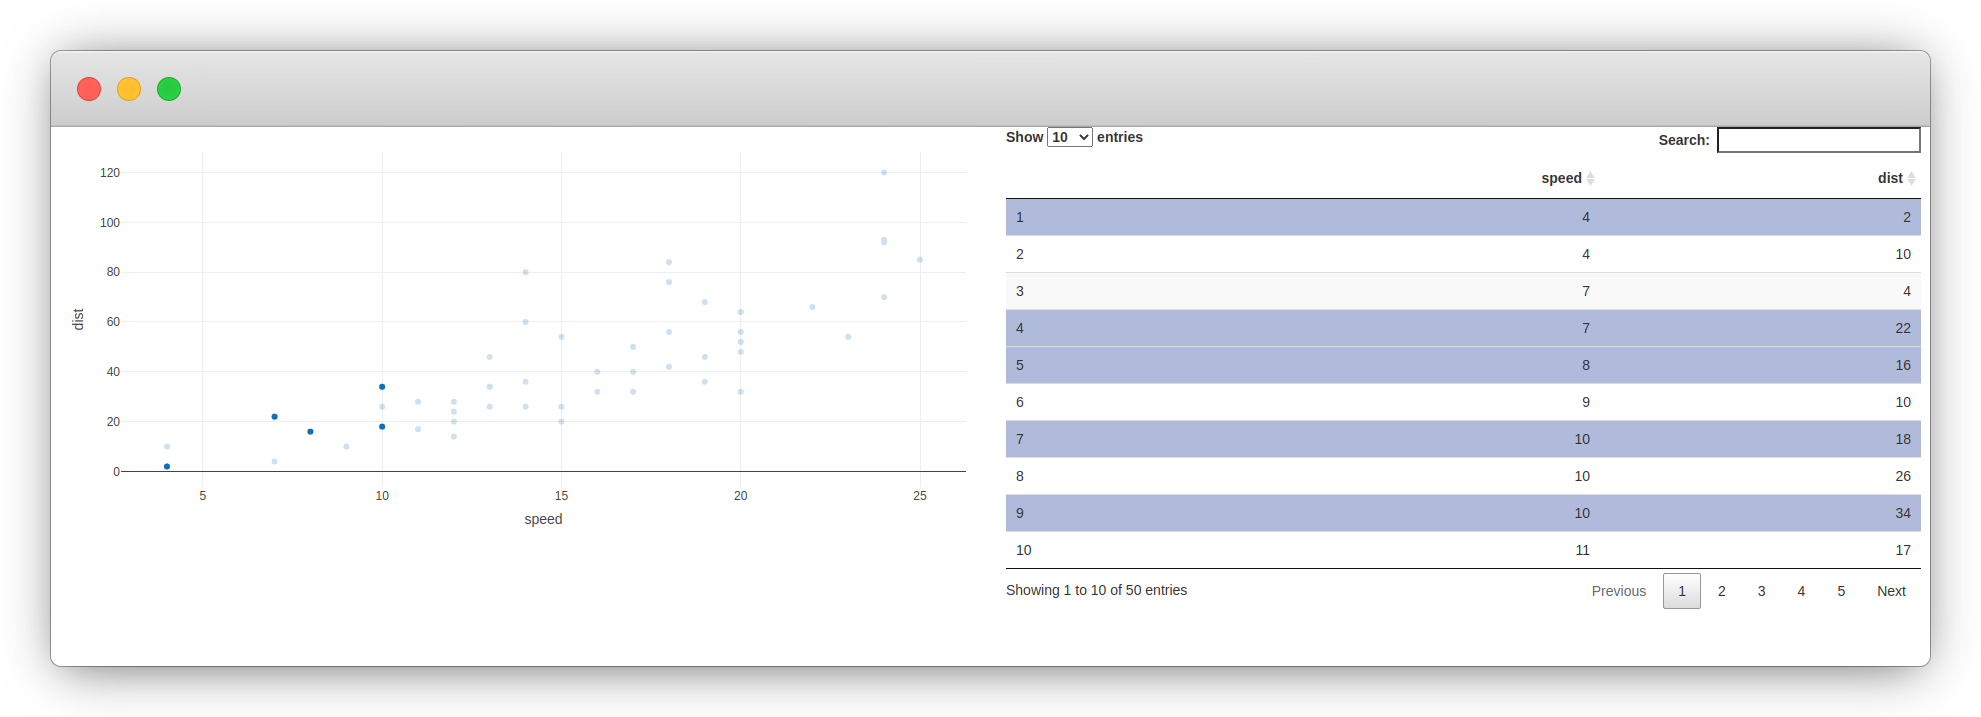
\includegraphics{images/crosstalk.png}
\caption{Crosstalk Example}
\end{figure}

With crosstalk comes the concept of ``groups,'' it defines an instance of shared data. The shared datasets created below will be linked because they share the same \texttt{group}, even though they are different R objects.

\begin{Shaded}
\begin{Highlighting}[]
\NormalTok{shared\_cars <{-}}\StringTok{ }\NormalTok{SharedData}\OperatorTok{$}\KeywordTok{new}\NormalTok{(mtcars, }\DataTypeTok{group =} \StringTok{"cars"}\NormalTok{)}
\NormalTok{shared\_cars\_head <{-}}\StringTok{ }\NormalTok{SharedData}\OperatorTok{$}\KeywordTok{new}\NormalTok{(}\KeywordTok{head}\NormalTok{(cars), }\DataTypeTok{group =} \StringTok{"cars"}\NormalTok{)}
\end{Highlighting}
\end{Shaded}

We will later explore and demonstrate why and where this is useful.

Basic usage of crosstalk datasets in shiny is very straightforward since it accepts reactive expressions to create shared datasets. Note that it takes the expression itself (\texttt{reactive}) not the output of the expression (\texttt{expression()}).

\begin{quote}
If this feels foreign to you, think of how you pass a function name, not a function call, to \texttt{lapply}; that's exactly analogous to what we're doing here.

\VA{--- Official Crosstalk documentation}{}
\end{quote}

\begin{Shaded}
\begin{Highlighting}[]
\KeywordTok{library}\NormalTok{(DT)}
\KeywordTok{library}\NormalTok{(shiny)}
\KeywordTok{library}\NormalTok{(plotly)}
\KeywordTok{library}\NormalTok{(crosstalk)}

\NormalTok{ui <{-}}\StringTok{ }\KeywordTok{fluidPage}\NormalTok{(}
  \KeywordTok{selectInput}\NormalTok{(}
    \StringTok{"specie"}\NormalTok{, }\StringTok{"Specie"}\NormalTok{, }
    \DataTypeTok{choices =} \KeywordTok{c}\NormalTok{(}\StringTok{"setosa"}\NormalTok{, }\StringTok{"versicolor"}\NormalTok{, }\StringTok{"virginica"}\NormalTok{)}
\NormalTok{  ),}
  \KeywordTok{fluidRow}\NormalTok{(}
    \KeywordTok{column}\NormalTok{(}\DecValTok{6}\NormalTok{, }\KeywordTok{DTOutput}\NormalTok{(}\StringTok{"table"}\NormalTok{)),}
    \KeywordTok{column}\NormalTok{(}\DecValTok{6}\NormalTok{, }\KeywordTok{plotlyOutput}\NormalTok{(}\StringTok{"plot"}\NormalTok{))}
\NormalTok{  )}
\NormalTok{)}

\NormalTok{server <{-}}\StringTok{ }\ControlFlowTok{function}\NormalTok{(input, output) \{}
\NormalTok{  reactive\_data <{-}}\StringTok{ }\KeywordTok{reactive}\NormalTok{(\{}
\NormalTok{    iris[iris}\OperatorTok{$}\NormalTok{Species }\OperatorTok{==}\StringTok{ }\NormalTok{input}\OperatorTok{$}\NormalTok{specie, ]}
\NormalTok{  \})}

\NormalTok{  sd <{-}}\StringTok{ }\NormalTok{SharedData}\OperatorTok{$}\KeywordTok{new}\NormalTok{(reactive\_data)}

\NormalTok{  output}\OperatorTok{$}\NormalTok{table <{-}}\StringTok{ }\KeywordTok{renderDT}\NormalTok{(\{}
    \KeywordTok{datatable}\NormalTok{(sd)}
\NormalTok{  \}, }\DataTypeTok{server =} \OtherTok{FALSE}\NormalTok{)}

\NormalTok{  output}\OperatorTok{$}\NormalTok{plot <{-}}\StringTok{ }\KeywordTok{renderPlotly}\NormalTok{(\{}
    \KeywordTok{plot\_ly}\NormalTok{(sd, }\DataTypeTok{x =} \OperatorTok{\textasciitilde{}}\NormalTok{Sepal.Length, }\DataTypeTok{y =} \OperatorTok{\textasciitilde{}}\NormalTok{Sepal.Width)}
\NormalTok{  \})}
\NormalTok{\}}

\KeywordTok{shinyApp}\NormalTok{(ui, server)}
\end{Highlighting}
\end{Shaded}

\begin{rmdnote}
Create the shared dataset in the server function or some things might
not work as expected in shiny.
\end{rmdnote}

One can also use the \texttt{data} method on the crosstalk object in reactive expressions, which allows accessing the Javascript selection where crosstalk is not directly supported, like below in a custom UI block. Note that the argument \texttt{withSelection} is set to \texttt{TRUE} in order to retrieve the selection state of the rows.

\begin{Shaded}
\begin{Highlighting}[]
\KeywordTok{library}\NormalTok{(DT)}
\KeywordTok{library}\NormalTok{(shiny)}
\KeywordTok{library}\NormalTok{(crosstalk)}

\NormalTok{ui <{-}}\StringTok{ }\KeywordTok{fluidPage}\NormalTok{(}
  \KeywordTok{fluidRow}\NormalTok{(}
    \KeywordTok{column}\NormalTok{(}\DecValTok{4}\NormalTok{, }\KeywordTok{uiOutput}\NormalTok{(}\StringTok{"text"}\NormalTok{)),}
    \KeywordTok{column}\NormalTok{(}\DecValTok{8}\NormalTok{, }\KeywordTok{DTOutput}\NormalTok{(}\StringTok{"table"}\NormalTok{))}
\NormalTok{  )}
\NormalTok{)}

\NormalTok{server <{-}}\StringTok{ }\ControlFlowTok{function}\NormalTok{(input, output) \{}
\NormalTok{  sd <{-}}\StringTok{ }\NormalTok{SharedData}\OperatorTok{$}\KeywordTok{new}\NormalTok{(cars)}

\NormalTok{  output}\OperatorTok{$}\NormalTok{text <{-}}\StringTok{ }\KeywordTok{renderUI}\NormalTok{(\{}
    \CommentTok{\# get selected rows}
\NormalTok{    n\_selected <{-}}\StringTok{ }\NormalTok{sd}\OperatorTok{$}\KeywordTok{data}\NormalTok{(}\DataTypeTok{withSelection =} \OtherTok{TRUE}\NormalTok{) }\OperatorTok{\%>\%}\StringTok{ }
\StringTok{      }\NormalTok{dplyr}\OperatorTok{::}\KeywordTok{filter}\NormalTok{(selected\_ }\OperatorTok{==}\StringTok{ }\OtherTok{TRUE}\NormalTok{) }\OperatorTok{\%>\%}\StringTok{ }
\StringTok{      }\KeywordTok{nrow}\NormalTok{()}

    \KeywordTok{h3}\NormalTok{(n\_selected, }\StringTok{"selected items"}\NormalTok{)}
    
\NormalTok{  \})}

\NormalTok{  output}\OperatorTok{$}\NormalTok{table <{-}}\StringTok{ }\KeywordTok{renderDT}\NormalTok{(\{}
    \KeywordTok{datatable}\NormalTok{(sd)}
\NormalTok{  \}, }\DataTypeTok{server =} \OtherTok{FALSE}\NormalTok{)}
\NormalTok{\}}

\KeywordTok{shinyApp}\NormalTok{(ui, server)}
\end{Highlighting}
\end{Shaded}

\begin{figure}
\centering
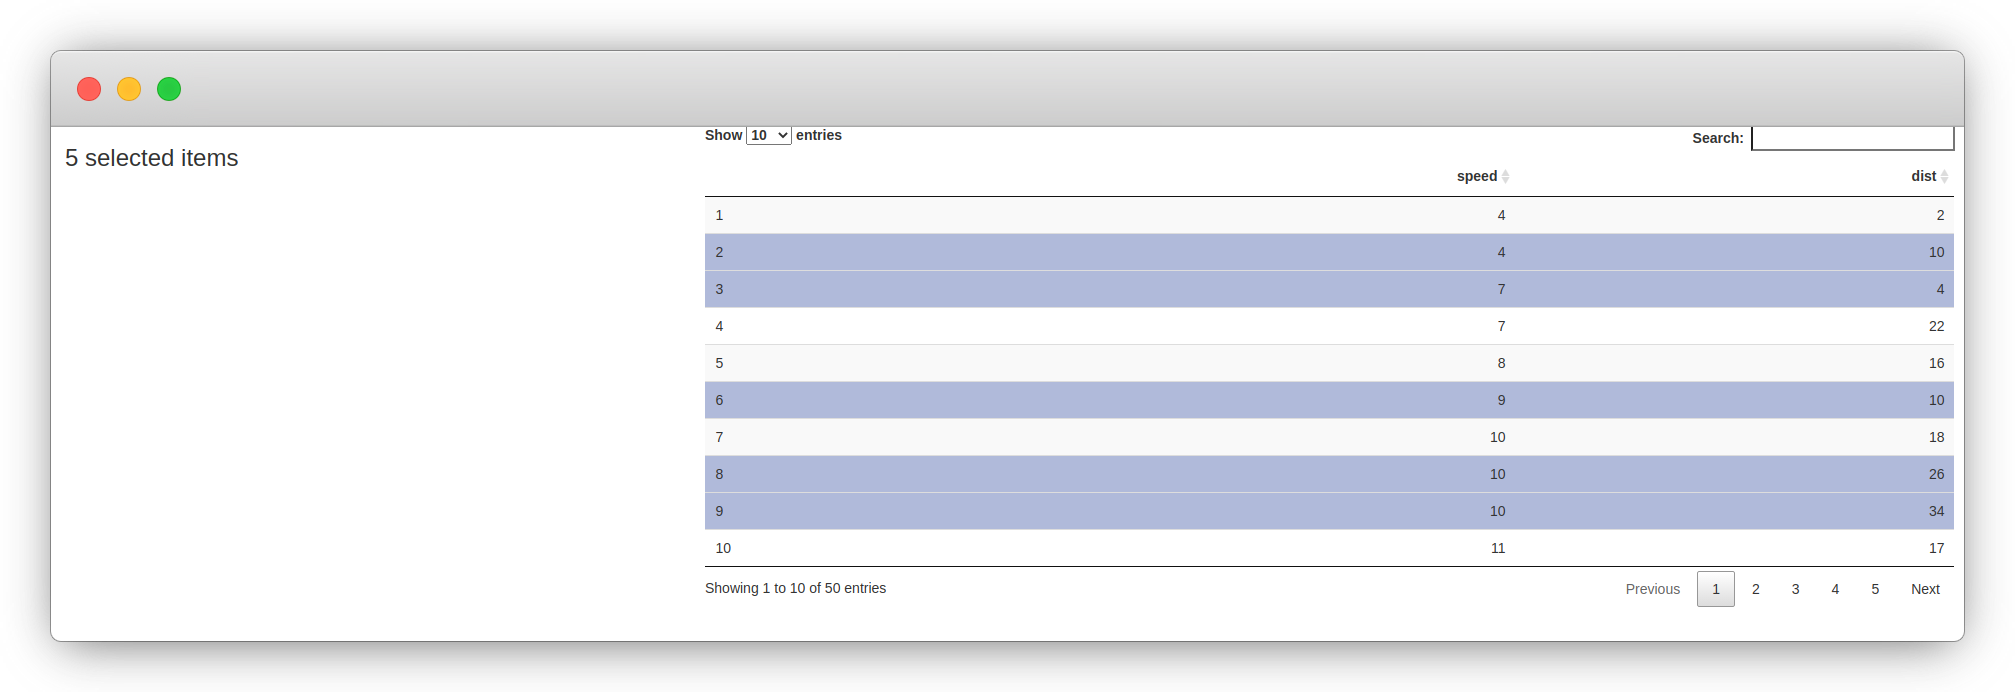
\includegraphics{images/crosstalk-shiny.png}
\caption{Shiny with crosstalk}
\end{figure}

Using crosstalk with shiny one can also change the selection server-side with the \texttt{selection} method, passing it the keys to select.

\begin{Shaded}
\begin{Highlighting}[]
\KeywordTok{library}\NormalTok{(DT)}
\KeywordTok{library}\NormalTok{(shiny)}
\KeywordTok{library}\NormalTok{(crosstalk)}

\NormalTok{ui <{-}}\StringTok{ }\KeywordTok{fluidPage}\NormalTok{(}
  \KeywordTok{fluidRow}\NormalTok{(}
    \KeywordTok{column}\NormalTok{(}\DecValTok{4}\NormalTok{, }\KeywordTok{actionButton}\NormalTok{(}\StringTok{"random"}\NormalTok{, }\StringTok{"Select a random row"}\NormalTok{)),}
    \KeywordTok{column}\NormalTok{(}\DecValTok{8}\NormalTok{, }\KeywordTok{DTOutput}\NormalTok{(}\StringTok{"table"}\NormalTok{))}
\NormalTok{  )}
\NormalTok{)}

\NormalTok{server <{-}}\StringTok{ }\ControlFlowTok{function}\NormalTok{(input, output) \{}
\NormalTok{  sd <{-}}\StringTok{ }\NormalTok{SharedData}\OperatorTok{$}\KeywordTok{new}\NormalTok{(cars)}

\NormalTok{  output}\OperatorTok{$}\NormalTok{table <{-}}\StringTok{ }\KeywordTok{renderDT}\NormalTok{(\{}
    \KeywordTok{datatable}\NormalTok{(sd)}
\NormalTok{  \}, }\DataTypeTok{server =} \OtherTok{FALSE}\NormalTok{)}

\NormalTok{  selected <{-}}\StringTok{ }\KeywordTok{c}\NormalTok{()}
  \KeywordTok{observeEvent}\NormalTok{(input}\OperatorTok{$}\NormalTok{random, \{}
\NormalTok{    smp <{-}}\StringTok{ }\KeywordTok{c}\NormalTok{(}\DecValTok{1}\OperatorTok{:}\DecValTok{50}\NormalTok{)[}\OperatorTok{!}\DecValTok{1}\OperatorTok{:}\DecValTok{50} \OperatorTok{\%in\%}\StringTok{ }\NormalTok{selected]}
\NormalTok{    selected <<{-}}\StringTok{ }\KeywordTok{append}\NormalTok{(selected, }\KeywordTok{sample}\NormalTok{(smp, }\DecValTok{1}\NormalTok{))}
\NormalTok{    sd}\OperatorTok{$}\KeywordTok{selection}\NormalTok{(selected)}
\NormalTok{  \})}
\NormalTok{\}}

\KeywordTok{shinyApp}\NormalTok{(ui, server)}
\end{Highlighting}
\end{Shaded}

\hypertarget{crosstalk-requirements}{%
\section{Crosstalk requirements}\label{crosstalk-requirements}}

Crosstalk is will not work well with every widget and every dataset, in some cases it might not even be a good idea to support it.

Crosstalk works best on rectangular data: dataframes or objects that resemble dataframes like \texttt{tibble} or \texttt{SpatialPolygonsDataFrame}. This is important as crosstalk will treat the data rowwise, where each row is an observation that is ultimately selected, or filtered. If the underlying data is not tabular (e.g.: trees) then one might eventually encounter mismatches between widgets.

Other than tabular data, crosstalk will require the widget to have the necessary functions or methods to dispatch the selection and filtering that crosstalk enables, that is, the widget must be able to filter as well as highlight and fade selected data points.

\hypertarget{how-it-works}{%
\section{How it works}\label{how-it-works}}

As will be discovered later when we bring crosstalk support to gio, very little changes on the R side. As might be expected, crosstalk enables communication between widgets via JavaScript, hence much of what must be adapted by widgets developers happens in JavaScript too.

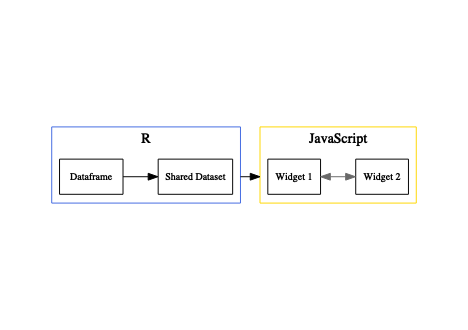
\includegraphics{bookdown_files/figure-latex/unnamed-chunk-35-1.png}

Indeed the biderectional communication between widgets works in the RStudio viewer, R markdown, Shiny and elsewhere, clearly indicating that all of it is taking place in the browser. This, internally, works with \texttt{key}s that are assigned to every row of the data.frame. These keys can be explicitly set by the user and otherwise default to the row names of the data.frame, and if these are not available will create row numbers.

\begin{Shaded}
\begin{Highlighting}[]
\CommentTok{\# assign keys}
\NormalTok{df <{-}}\StringTok{ }\KeywordTok{data.frame}\NormalTok{(}\DataTypeTok{x =} \KeywordTok{runif}\NormalTok{(}\DecValTok{26}\NormalTok{))}
\NormalTok{sd <{-}}\StringTok{ }\NormalTok{SharedData}\OperatorTok{$}\KeywordTok{new}\NormalTok{(df, }\DataTypeTok{key =}\NormalTok{ letters)}
\end{Highlighting}
\end{Shaded}

In a sense, while crosstalk handles the lines of communication between widgets, developers of the respective widgets must handle what messages are sent to others and what to do with messages coming from other widgets. There are two types of such messages: filtering to actually narrow down the selection of data points displayed on a widget, and selection (what crosstalk refers to as ``linked brushing'') to highlight certain data points.

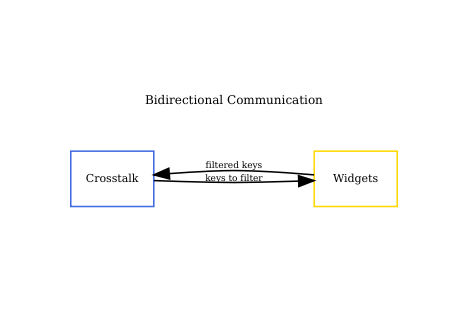
\includegraphics{bookdown_files/figure-latex/unnamed-chunk-37-1.png}

This selection or filtering is communicated with the aforementioned keys. In JavaScript, a widget ``receives'' the keys of selected and filtered data points and must, when filtering or selection is observed, ``send'' said selected or filtered keys to other widgets.

Internally crosstalk knows what to share across widgets with the aforementioned \texttt{group}, each group is isolated from each other so one can use multiple different shared datasets without them interfering with each other.

\hypertarget{crosstalk-with-gio}{%
\section{Crosstalk with gio}\label{crosstalk-with-gio}}

The application of crosstalk to the gio library is somewhat amiss. As mentioned or hinted at before, in order for crosstalk to be properly implemented a widget must be a able to select, deselect as well as filter and unfilter data points and this is not entirely the case of gio.

\begin{rmdnote}
The application of crosstalk to the gio package is instructive but
limited and somewhat faulty.
\end{rmdnote}

First, gio's underlying data is somewhat uncommon: it is a network defined only by its edges (the arcs leaving and coming into countries). Second, those edges themselves cannot be selected, as we've observed previously one cannot truly change what edges are drawn on the globe, only change which country is selected and by proxy which edges are shown. Third, while gio supports changing which country is selected it does not allow having not countries selected.

The way crosstalk can work with gio is by setting the keys of the shared dataset to the country ISO codes that gio uses. Since data gio accepts consists of edges this ISO code could correspond to either source or the target country.

\begin{Shaded}
\begin{Highlighting}[]
\NormalTok{shared\_arcs <{-}}\StringTok{ }\NormalTok{SharedData}\OperatorTok{$}\KeywordTok{new}\NormalTok{(arcs, }\DataTypeTok{key =}\NormalTok{ arcs}\OperatorTok{$}\NormalTok{i)}
\end{Highlighting}
\end{Shaded}

\hypertarget{adapt-the-r-code}{%
\section{Adapt the R code}\label{adapt-the-r-code}}

In any event, let us start by making the required changes to the R code first. The only changes that need to be made are in the \texttt{gio} function as it is the only that accepts a data object.

\begin{Shaded}
\begin{Highlighting}[]
\KeywordTok{class}\NormalTok{(shared\_arcs)}
\end{Highlighting}
\end{Shaded}

\begin{verbatim}
## [1] "SharedData" "R6"
\end{verbatim}

The shared datasets are R6 classes and therefore cannot simply be treated as dataframes. The \texttt{gio} function needs to check whether the \texttt{data} object it received is a shared dataset with \texttt{is.SharedData} and if so use its methods to extract data from it, namely:

\begin{itemize}
\tightlist
\item
  The original dataset with \texttt{origData}.
\item
  The group to which the dataset belongs with \texttt{groupName}.
\item
  The keys that were assigned to every row of the dataset with \texttt{key}
\end{itemize}

\begin{Shaded}
\begin{Highlighting}[]
\CommentTok{\# original data}
\NormalTok{shared\_arcs}\OperatorTok{$}\KeywordTok{origData}\NormalTok{()}
\end{Highlighting}
\end{Shaded}

\begin{verbatim}
##    e  i       v
## 1 CN US 3300000
## 2 CN RU   10000
\end{verbatim}

Note that the name of the group was randomly generated since none were specified when the shared dataset was created.

\begin{Shaded}
\begin{Highlighting}[]
\CommentTok{\# groupName}
\NormalTok{shared\_arcs}\OperatorTok{$}\KeywordTok{groupName}\NormalTok{()}
\end{Highlighting}
\end{Shaded}

\begin{verbatim}
## [1] "SharedData0a55b526"
\end{verbatim}

\begin{Shaded}
\begin{Highlighting}[]
\CommentTok{\# keys}
\NormalTok{shared\_arcs}\OperatorTok{$}\KeywordTok{key}\NormalTok{()}
\end{Highlighting}
\end{Shaded}

\begin{verbatim}
## [1] "US" "RU"
\end{verbatim}

The methods \texttt{origData} and \texttt{groupName} must be used in every widget, the original dataframe is still needed to produce the visualisation and the group will be needed JavaScript so we can tell crosstalk which group one is working with. The \texttt{key} method may not be useful with every widget if the visualisation library also comes with a key/id system so one can use it internally, we won't be using it with gio. Finally notice that we also add the JavaScript dependency with \texttt{crosstalkLibs}.

\begin{Shaded}
\begin{Highlighting}[]
\NormalTok{gio <{-}}\StringTok{ }\ControlFlowTok{function}\NormalTok{(data, }\DataTypeTok{width =} \OtherTok{NULL}\NormalTok{, }\DataTypeTok{height =} \OtherTok{NULL}\NormalTok{, }
  \DataTypeTok{elementId =} \OtherTok{NULL}\NormalTok{) \{}

  \CommentTok{\# defaults to NULL}
\NormalTok{  group <{-}}\StringTok{ }\OtherTok{NULL}

  \CommentTok{\# uses crosstalk}
  \ControlFlowTok{if}\NormalTok{ (crosstalk}\OperatorTok{::}\KeywordTok{is.SharedData}\NormalTok{(data)) \{}
\NormalTok{    group <{-}}\StringTok{ }\NormalTok{data}\OperatorTok{$}\KeywordTok{groupName}\NormalTok{()}
\NormalTok{    data <{-}}\StringTok{ }\NormalTok{data}\OperatorTok{$}\KeywordTok{origData}\NormalTok{()}
\NormalTok{  \}}

  \CommentTok{\# forward options using x}
\NormalTok{  x =}\StringTok{ }\KeywordTok{list}\NormalTok{(}
    \DataTypeTok{data =}\NormalTok{ data,}
    \DataTypeTok{style =} \StringTok{"default"}\NormalTok{,}
    \DataTypeTok{crosstalk =} \KeywordTok{list}\NormalTok{(}\DataTypeTok{group =}\NormalTok{ group) }\CommentTok{\# pass group}
\NormalTok{  )}

  \KeywordTok{attr}\NormalTok{(x, }\StringTok{\textquotesingle{}TOJSON\_ARGS\textquotesingle{}}\NormalTok{) <{-}}\StringTok{ }\KeywordTok{list}\NormalTok{(}\DataTypeTok{dataframe =} \StringTok{"rows"}\NormalTok{)}

  \CommentTok{\# create widget}
\NormalTok{  htmlwidgets}\OperatorTok{::}\KeywordTok{createWidget}\NormalTok{(}
    \DataTypeTok{name =} \StringTok{\textquotesingle{}gio\textquotesingle{}}\NormalTok{,}
\NormalTok{    x,}
    \DataTypeTok{width =}\NormalTok{ width,}
    \DataTypeTok{height =}\NormalTok{ height,}
    \DataTypeTok{package =} \StringTok{\textquotesingle{}gio\textquotesingle{}}\NormalTok{,}
    \DataTypeTok{elementId =}\NormalTok{ elementId,}
    \DataTypeTok{sizingPolicy =}\NormalTok{ htmlwidgets}\OperatorTok{::}\KeywordTok{sizingPolicy}\NormalTok{(}
      \DataTypeTok{padding =} \DecValTok{0}\NormalTok{,}
      \DataTypeTok{browser.fill =} \OtherTok{TRUE}\NormalTok{,}
      \DataTypeTok{defaultWidth =} \StringTok{"100\%"}
\NormalTok{    ),}
    \DataTypeTok{preRenderHook =}\NormalTok{ render\_gio,}
    \CommentTok{\# add crosstalk dependency}
    \DataTypeTok{dependencies =}\NormalTok{ crosstalk}\OperatorTok{::}\KeywordTok{crosstalkLibs}\NormalTok{()}
\NormalTok{  )}
\NormalTok{\}}
\end{Highlighting}
\end{Shaded}

The widget will now ship with the crosstalk dependencies and the group name will be serialised and accessible in JavaScript.

\hypertarget{change-the-javascript-code}{%
\section{Change the JavaScript code}\label{change-the-javascript-code}}

What is left to do is to adapt the JavaScript code, as mentioned previously it must accept the keys selected in other widgets and share the selected key with other widgets.

First we create the selection handler in the \texttt{factory} function, this is done by instantiating a new class from \texttt{crosstalk.SelectionHandle}.

\begin{Shaded}
\begin{Highlighting}[]
\KeywordTok{var}\NormalTok{ sel\_handle }\OperatorTok{=} \KeywordTok{new} \VariableTok{crosstalk}\NormalTok{.}\AttributeTok{SelectionHandle}\NormalTok{()}\OperatorTok{;}
\end{Highlighting}
\end{Shaded}

Once the selection handle created it can be used in the \texttt{renderValue} function to define set the group.

\begin{Shaded}
\begin{Highlighting}[]
\VariableTok{sel\_handle}\NormalTok{.}\AttributeTok{setGroup}\NormalTok{(}\VariableTok{x}\NormalTok{.}\VariableTok{crosstalk}\NormalTok{.}\AttributeTok{group}\NormalTok{)}\OperatorTok{;}
\end{Highlighting}
\end{Shaded}

\hypertarget{send-selected-keys}{%
\subsection{Send selected keys}\label{send-selected-keys}}

In order to send the selected keys to crosstalk we shall need to use the one callback function that gio allows using. This callback function is fired every time a user selects a country on the globe and accepts two arguments, one containing data on the country selected and another containing data on the related countries (the arcs coming and leaving the selected country). For this exercise only the selected country is of use. The callback function that one wants to have run every time a country is picked by the user can be passed to \texttt{controller.onCountryPicked}

Let us first explore the what is within the object \texttt{selectedCountry} object by logging it to the console.

\begin{Shaded}
\begin{Highlighting}[]
\CommentTok{// placed in renderValue function}

\CommentTok{// create callback function}
\KeywordTok{function} \AttributeTok{callback}\NormalTok{ (selectedCountry) }\OperatorTok{\{}
  \VariableTok{console}\NormalTok{.}\AttributeTok{log}\NormalTok{(selectedCountry)}\OperatorTok{;}
\OperatorTok{\}}

\CommentTok{// pass it to gio.js}
\VariableTok{controller}\NormalTok{.}\AttributeTok{onCountryPicked}\NormalTok{(callback)}\OperatorTok{;}
\end{Highlighting}
\end{Shaded}

\begin{Shaded}
\begin{Highlighting}[]
\FunctionTok{\{}\ErrorTok{name}\FunctionTok{:} \StringTok{"LIBYA"}\FunctionTok{,} \ErrorTok{lat}\FunctionTok{:} \DecValTok{25}\FunctionTok{,} \ErrorTok{lon}\FunctionTok{:} \DecValTok{17}\FunctionTok{,} \ErrorTok{center}\FunctionTok{:} \ErrorTok{n}\FunctionTok{,} \ErrorTok{ISOCode}\FunctionTok{:} \StringTok{"LY"}\FunctionTok{\}}
\end{Highlighting}
\end{Shaded}

As mentioned at the beginning of this section, the keys used with the datasets for gio.js should be ISO codes, therefore one can consider the \texttt{ISOCode} variable as selected \texttt{key}. The \texttt{set} method from the selection handle can be used to share the selected key with other widgets. Note that this method expects either a \texttt{null} value or an array a scalar value will throw an error, hence \texttt{selectedCountry.ISOCode} is wrapped in square brackets.

\begin{Shaded}
\begin{Highlighting}[]
\KeywordTok{function} \AttributeTok{callback}\NormalTok{ (selectedCountry) }\OperatorTok{\{}
  \VariableTok{sel\_handle}\NormalTok{.}\AttributeTok{set}\NormalTok{([}\VariableTok{selectedCountry}\NormalTok{.}\AttributeTok{ISOCode}\NormalTok{])}\OperatorTok{;}
\OperatorTok{\}}

\VariableTok{controller}\NormalTok{.}\AttributeTok{onCountryPicked}\NormalTok{(callback)}\OperatorTok{;}
\end{Highlighting}
\end{Shaded}

\hypertarget{set-selected-keys}{%
\subsection{Set selected keys}\label{set-selected-keys}}

We have implemented the necessary to share the selected country with other widgets but are yet to implemented the opposite; when users select a country in another widget the selected country in gio should change too.

\begin{Shaded}
\begin{Highlighting}[]
\CommentTok{// placed in factory function}
\VariableTok{sel\_handle}\NormalTok{.}\AttributeTok{on}\NormalTok{(}\StringTok{"change"}\OperatorTok{,} \KeywordTok{function}\NormalTok{(e) }\OperatorTok{\{}
  \VariableTok{console}\NormalTok{.}\AttributeTok{log}\NormalTok{(e)}\OperatorTok{;}
\OperatorTok{\}}\NormalTok{)}\OperatorTok{;}
\end{Highlighting}
\end{Shaded}

\begin{Shaded}
\begin{Highlighting}[]
\FunctionTok{\{}
  \ErrorTok{oldValue}\FunctionTok{:} \OtherTok{[]}\FunctionTok{,}
  \ErrorTok{sender}\FunctionTok{:} \ErrorTok{n} \FunctionTok{\{}
    \ErrorTok{\_eventRelay}\FunctionTok{:} \ErrorTok{e}\FunctionTok{,} 
    \ErrorTok{\_emitter}\FunctionTok{:} \ErrorTok{t}\FunctionTok{,} 
    \ErrorTok{\_group}\FunctionTok{:} \StringTok{"SharedDatac7682f87"}\FunctionTok{,} 
    \ErrorTok{\_var}\FunctionTok{:} \ErrorTok{r}\FunctionTok{,} 
    \ErrorTok{\_varOnChangeSub}\FunctionTok{:} \StringTok{"sub1"}\FunctionTok{,} 
    \ErrorTok{…}
  \FunctionTok{\},}
  \ErrorTok{value}\FunctionTok{:} \OtherTok{[}\StringTok{"AE"}\OtherTok{]}
\FunctionTok{\}}
\end{Highlighting}
\end{Shaded}

\begin{enumerate}
\def\labelenumi{\arabic{enumi}.}
\tightlist
\item
  \texttt{oldValue} - the value that was previously selected (if any), this may be useful if the widget wants to calculate differences between the currently and previously selected value.
\item
  \texttt{sender} - the selection handle instance that made the change. This is useful to compare against the selection handle of the widget and know whether the change in selection was initiated by this widget or another. It is often used to clear the selection or filtering before applying a new one when the change comes from another widget.
\item
  \texttt{value} - the array of selected keys.
\end{enumerate}

Therefore the listening to the change event on the selection would look like this. Note that 1) the selection cannot be cleared with gio.js, a country is always selected, and 2) one can only select one country a time, hence only accepting the first element of the selected keys with \texttt{e.value{[}0{]}}.

\begin{Shaded}
\begin{Highlighting}[]
\CommentTok{// placed in factory function}
\VariableTok{sel\_handle}\NormalTok{.}\AttributeTok{on}\NormalTok{(}\StringTok{"change"}\OperatorTok{,} \KeywordTok{function}\NormalTok{(e) }\OperatorTok{\{}
  \ControlFlowTok{if}\NormalTok{ (}\VariableTok{e}\NormalTok{.}\AttributeTok{sender} \OperatorTok{!==}\NormalTok{ sel\_handle) }\OperatorTok{\{}
    \CommentTok{// clear the selection}
    \CommentTok{// not possible with gio.js}
  \OperatorTok{\}}
  \VariableTok{controller}\NormalTok{.}\AttributeTok{switchCountry}\NormalTok{(}\VariableTok{e}\NormalTok{.}\AttributeTok{value}\NormalTok{[}\DecValTok{0}\NormalTok{])}\OperatorTok{;}
\OperatorTok{\}}\NormalTok{)}\OperatorTok{;}
\end{Highlighting}
\end{Shaded}

To recap, this is what the JavaScript code should not look like.

\begin{Shaded}
\begin{Highlighting}[]
\VariableTok{HTMLWidgets}\NormalTok{.}\AttributeTok{widget}\NormalTok{(}\OperatorTok{\{}

  \DataTypeTok{name}\OperatorTok{:} \StringTok{\textquotesingle{}gio\textquotesingle{}}\OperatorTok{,}

  \DataTypeTok{type}\OperatorTok{:} \StringTok{\textquotesingle{}output\textquotesingle{}}\OperatorTok{,}

  \DataTypeTok{factory}\OperatorTok{:} \KeywordTok{function}\NormalTok{(el}\OperatorTok{,}\NormalTok{ width}\OperatorTok{,}\NormalTok{ height) }\OperatorTok{\{}

    \CommentTok{// }\AlertTok{TODO}\CommentTok{: define shared variables for this instance}
    \KeywordTok{var}\NormalTok{ controller}\OperatorTok{;}

    \CommentTok{// create selection handle}
    \KeywordTok{var}\NormalTok{ sel\_handle }\OperatorTok{=} \KeywordTok{new} \VariableTok{crosstalk}\NormalTok{.}\AttributeTok{SelectionHandle}\NormalTok{()}\OperatorTok{;}

    \CommentTok{// listen to change}
    \VariableTok{sel\_handle}\NormalTok{.}\AttributeTok{on}\NormalTok{(}\StringTok{"change"}\OperatorTok{,} \KeywordTok{function}\NormalTok{(e) }\OperatorTok{\{}
      \ControlFlowTok{if}\NormalTok{ (}\VariableTok{e}\NormalTok{.}\AttributeTok{sender} \OperatorTok{!==}\NormalTok{ sel\_handle) }\OperatorTok{\{}
        \CommentTok{// clear selection}
      \OperatorTok{\}}
      \VariableTok{controller}\NormalTok{.}\AttributeTok{switchCountry}\NormalTok{(}\VariableTok{e}\NormalTok{.}\AttributeTok{value}\NormalTok{[}\DecValTok{0}\NormalTok{])}\OperatorTok{;}
    \OperatorTok{\}}\NormalTok{)}\OperatorTok{;}


    \ControlFlowTok{return} \OperatorTok{\{}

      \DataTypeTok{renderValue}\OperatorTok{:} \KeywordTok{function}\NormalTok{(x) }\OperatorTok{\{}

\NormalTok{        controller }\OperatorTok{=} \KeywordTok{new} \VariableTok{GIO}\NormalTok{.}\AttributeTok{Controller}\NormalTok{(el)}\OperatorTok{;}

        \CommentTok{// group}
        \VariableTok{sel\_handle}\NormalTok{.}\AttributeTok{setGroup}\NormalTok{(}\VariableTok{x}\NormalTok{.}\VariableTok{crosstalk}\NormalTok{.}\AttributeTok{group}\NormalTok{)}\OperatorTok{;}
        
        \CommentTok{// add data}
        \VariableTok{controller}\NormalTok{.}\AttributeTok{addData}\NormalTok{(}\VariableTok{x}\NormalTok{.}\AttributeTok{data}\NormalTok{)}\OperatorTok{;}

        \VariableTok{controller}\NormalTok{.}\AttributeTok{setStyle}\NormalTok{(}\VariableTok{x}\NormalTok{.}\AttributeTok{style}\NormalTok{)}\OperatorTok{;}

        \CommentTok{// callback}
        \KeywordTok{function} \AttributeTok{callback}\NormalTok{ (selectedCountry}\OperatorTok{,}\NormalTok{ relatedCountries) }\OperatorTok{\{}
          \VariableTok{sel\_handle}\NormalTok{.}\AttributeTok{set}\NormalTok{([}\VariableTok{selectedCountry}\NormalTok{.}\AttributeTok{ISOCode}\NormalTok{])}\OperatorTok{;} \CommentTok{// send keys}
        \OperatorTok{\}}

        \VariableTok{controller}\NormalTok{.}\AttributeTok{onCountryPicked}\NormalTok{(callback)}\OperatorTok{;}

        \CommentTok{// use stats}
        \ControlFlowTok{if}\NormalTok{(}\VariableTok{x}\NormalTok{.}\AttributeTok{stats}\NormalTok{)}
          \VariableTok{controller}\NormalTok{.}\AttributeTok{enableStats}\NormalTok{()}\OperatorTok{;}

        \CommentTok{// render}
        \VariableTok{controller}\NormalTok{.}\AttributeTok{init}\NormalTok{()}\OperatorTok{;}

      \OperatorTok{\},}

      \DataTypeTok{resize}\OperatorTok{:} \KeywordTok{function}\NormalTok{(width}\OperatorTok{,}\NormalTok{ height) }\OperatorTok{\{}
        \VariableTok{controller}\NormalTok{.}\AttributeTok{resizeUpdate}\NormalTok{()}\OperatorTok{;}
      \OperatorTok{\},}

    \OperatorTok{\};}
  \OperatorTok{\}}
\OperatorTok{\}}\NormalTok{)}\OperatorTok{;}
\end{Highlighting}
\end{Shaded}

\hypertarget{using-crosstalk-with-gio}{%
\subsection{Using crosstalk with gio}\label{using-crosstalk-with-gio}}

Finally, now that gio supports we can create a few examples to demonstrate how it can be used.

The simplest way is probably to convert the edges to a shared dataset specifying either the source (\texttt{i}) or target (\texttt{e}) country codes as keys. However this is unlikely to be used this way out in the real world. In the example below selecting an edge highlights a node which is somewhat confusing.

\begin{Shaded}
\begin{Highlighting}[]
\KeywordTok{library}\NormalTok{(DT)}
\KeywordTok{library}\NormalTok{(gio)}
\KeywordTok{library}\NormalTok{(crosstalk)}

\NormalTok{url <{-}}\StringTok{ }\KeywordTok{paste0}\NormalTok{(}
  \StringTok{"https://raw.githubusercontent.com/JohnCoene/"}\NormalTok{,}
  \StringTok{"javascript{-}for{-}r/master/data/countries.json"}
\NormalTok{)}
\NormalTok{arcs <{-}}\StringTok{ }\NormalTok{jsonlite}\OperatorTok{::}\KeywordTok{fromJSON}\NormalTok{(url)}

\CommentTok{\# Wrap data frame in SharedData}
\CommentTok{\# key is importing country}
\NormalTok{sd <{-}}\StringTok{ }\NormalTok{SharedData}\OperatorTok{$}\KeywordTok{new}\NormalTok{(arcs, }\DataTypeTok{key =}\NormalTok{ arcs}\OperatorTok{$}\NormalTok{i)}

\KeywordTok{bscols}\NormalTok{(}
  \KeywordTok{gio}\NormalTok{(sd),}
  \KeywordTok{datatable}\NormalTok{(sd, }\DataTypeTok{width=}\StringTok{"100\%"}\NormalTok{, }\DataTypeTok{selection =} \StringTok{"single"}\NormalTok{)}
\NormalTok{)}
\end{Highlighting}
\end{Shaded}

\begin{figure}
\centering
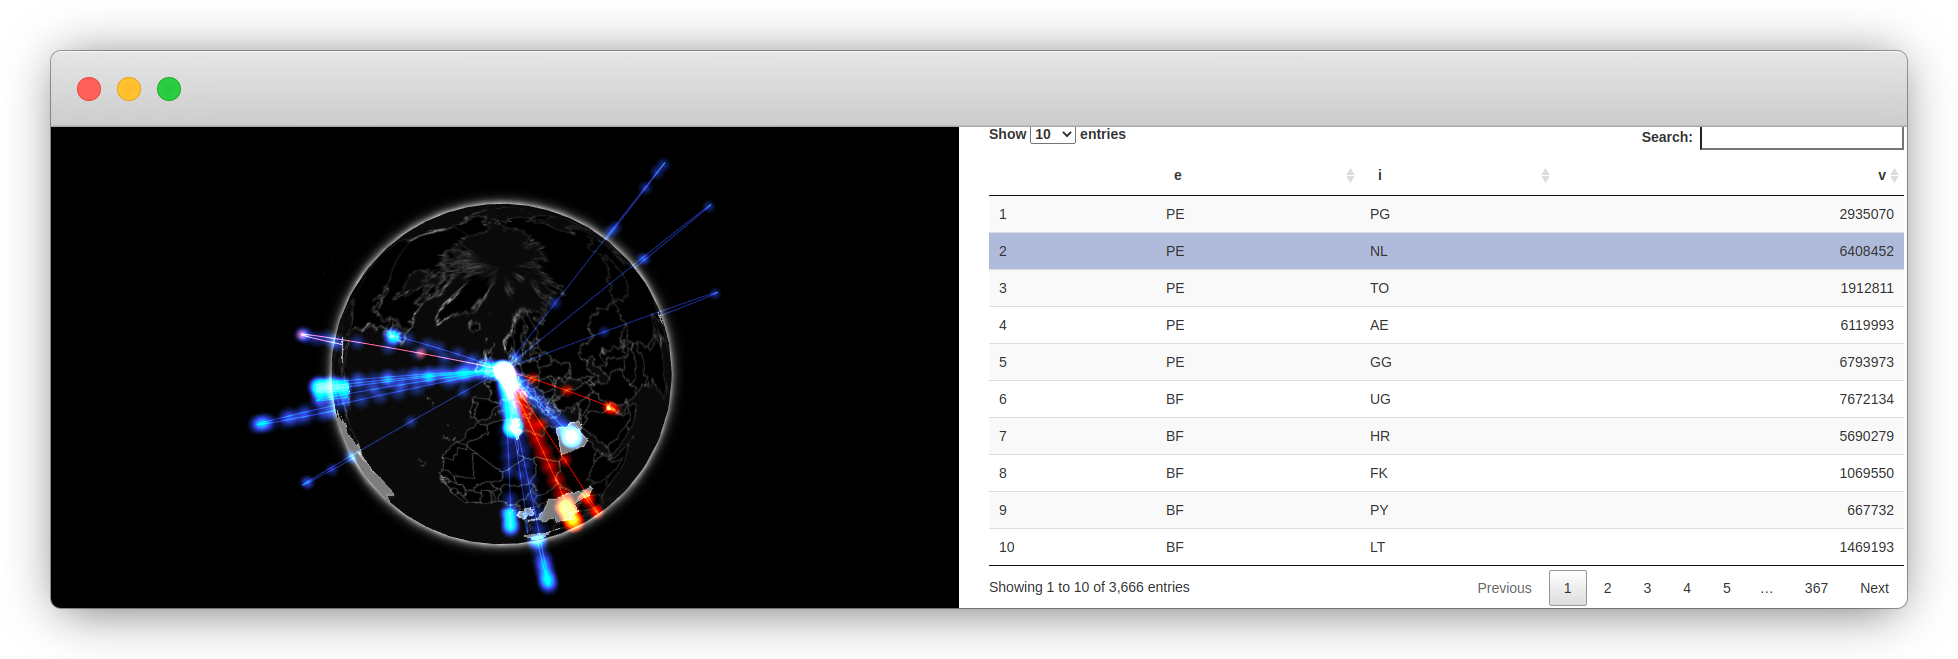
\includegraphics{images/crosstalk-gio-1.png}
\caption{Gio with DT using crosstalk}
\end{figure}

Thankfully we can use the \texttt{group} argument in order to create edges and nodes that share keys and produce a more sensible linkage. Below we create two shared datasets with the same group name, one for the edges and another for the nodes and use one for the gio visualisation and the other for the plotly graph.

\begin{Shaded}
\begin{Highlighting}[]
\KeywordTok{library}\NormalTok{(gio)}
\KeywordTok{library}\NormalTok{(plotly)}
\KeywordTok{library}\NormalTok{(crosstalk)}

\NormalTok{url <{-}}\StringTok{ }\KeywordTok{paste0}\NormalTok{(}
  \StringTok{"https://raw.githubusercontent.com/JohnCoene/"}\NormalTok{,}
  \StringTok{"javascript{-}for{-}r/master/data/countries.json"}
\NormalTok{)}
\NormalTok{arcs <{-}}\StringTok{ }\NormalTok{jsonlite}\OperatorTok{::}\KeywordTok{fromJSON}\NormalTok{(url)}

\CommentTok{\# Wrap data frame in SharedData}
\NormalTok{edges\_sd <{-}}\StringTok{ }\NormalTok{SharedData}\OperatorTok{$}\KeywordTok{new}\NormalTok{(arcs, }\DataTypeTok{key =}\NormalTok{ arcs}\OperatorTok{$}\NormalTok{i, }\DataTypeTok{group =} \StringTok{"gio"}\NormalTok{)}

\CommentTok{\# create nodes}
\NormalTok{iso2c <{-}}\StringTok{ }\KeywordTok{unique}\NormalTok{(arcs}\OperatorTok{$}\NormalTok{i)}
\NormalTok{nodes <{-}}\StringTok{ }\KeywordTok{data.frame}\NormalTok{(}
  \DataTypeTok{country =}\NormalTok{ iso2c,}
  \DataTypeTok{y =} \KeywordTok{rnorm}\NormalTok{(}\KeywordTok{length}\NormalTok{(iso2c))}
\NormalTok{)}
\NormalTok{nodes\_sd <{-}}\StringTok{ }\NormalTok{SharedData}\OperatorTok{$}\KeywordTok{new}\NormalTok{(}
\NormalTok{  nodes, }\DataTypeTok{key =}\NormalTok{ nodes}\OperatorTok{$}\NormalTok{country, }
  \DataTypeTok{group =} \StringTok{"gio"}
\NormalTok{)}

\KeywordTok{bscols}\NormalTok{(}
  \KeywordTok{plot\_ly}\NormalTok{(}\DataTypeTok{data =}\NormalTok{ nodes\_sd, }\DataTypeTok{type =} \StringTok{"bar"}\NormalTok{, }\DataTypeTok{x =} \OperatorTok{\textasciitilde{}}\NormalTok{country, }\DataTypeTok{y =} \OperatorTok{\textasciitilde{}}\NormalTok{y) }\OperatorTok{\%>\%}\StringTok{ }
\StringTok{    }\KeywordTok{config}\NormalTok{(}\DataTypeTok{displayModeBar =} \OtherTok{FALSE}\NormalTok{),}
  \KeywordTok{gio}\NormalTok{(edges\_sd)}
\NormalTok{)}
\end{Highlighting}
\end{Shaded}

\begin{figure}
\centering
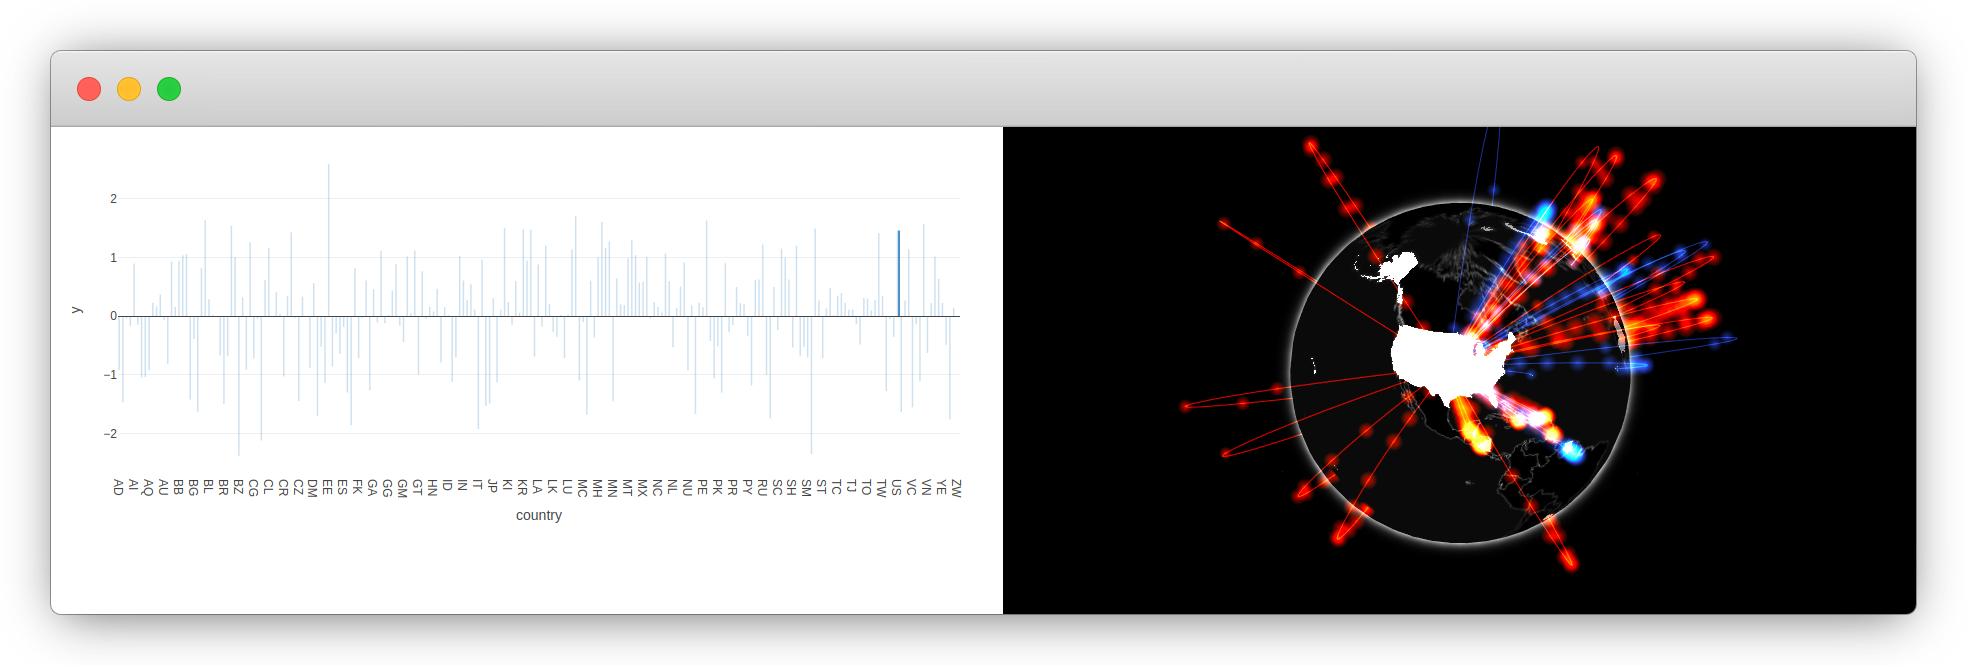
\includegraphics{images/crosstalk-gio-2.png}
\caption{Gio with DT and plotly using crosstalk}
\end{figure}

\hypertarget{final-revisions}{%
\chapter{Final Revisions}\label{final-revisions}}

In this chapter we polish the API that gio presents its users and provide guidelines to best integrate other JavaScript libraries with R.

\hypertarget{working-with-data}{%
\section{Working with data}\label{working-with-data}}

The gio package built thus far revolves around the \texttt{gio} function which expects a dataframe with three columns named \texttt{e}, \texttt{i}, and \texttt{v}, which is not great practice; there are great reasons why very few functions do that.

First, it is unlikely that one comes across a dataset with such names in the real world thus users of the package will likely need to rename the columns of the dataset in order to use gio making the package rather unwieldy. Second, this makes understanding and approaching the gio package more complicated, it will not be evident by looking at the examples, and usage of gio.

Instead \texttt{gio} should accept the dataframe as first argument and then the relevant columns to extract. This can be implemented in many ways ranging from arguments that accept the column names as strings to reproducing ggplot2's \texttt{aes} function. Below we settle for a solution probably lying somewhere in between: using non-standard evaluation to provide arguments that accept the bare name of the columns.

\begin{Shaded}
\begin{Highlighting}[]
\NormalTok{gio <{-}}\StringTok{ }\ControlFlowTok{function}\NormalTok{(data, source, target, value, ..., }
  \DataTypeTok{width =} \OtherTok{NULL}\NormalTok{, }\DataTypeTok{height =} \OtherTok{NULL}\NormalTok{, }\DataTypeTok{elementId =} \OtherTok{NULL}\NormalTok{) \{}

  \CommentTok{\# defaults to NULL}
\NormalTok{  group <{-}}\StringTok{ }\OtherTok{NULL}

  \ControlFlowTok{if}\NormalTok{ (crosstalk}\OperatorTok{::}\KeywordTok{is.SharedData}\NormalTok{(data)) \{}
\NormalTok{    group <{-}}\StringTok{ }\NormalTok{data}\OperatorTok{$}\KeywordTok{groupName}\NormalTok{()}
\NormalTok{    data <{-}}\StringTok{ }\NormalTok{data}\OperatorTok{$}\KeywordTok{origData}\NormalTok{()}
\NormalTok{  \}}

\NormalTok{  data <{-}}\StringTok{ }\NormalTok{dplyr}\OperatorTok{::}\KeywordTok{select}\NormalTok{(}
\NormalTok{    data,}
    \DataTypeTok{i =}\NormalTok{ \{\{ source \}\},}
    \DataTypeTok{e =}\NormalTok{ \{\{ target \}\},}
    \DataTypeTok{v =}\NormalTok{ \{\{ value \}\}}
\NormalTok{  )}

  \CommentTok{\# forward options using x}
\NormalTok{  x =}\StringTok{ }\KeywordTok{list}\NormalTok{(}
    \DataTypeTok{configs =} \KeywordTok{list}\NormalTok{(...),}
    \DataTypeTok{data =}\NormalTok{ data,}
    \DataTypeTok{style =} \StringTok{"default"}\NormalTok{,}
    \DataTypeTok{crosstalk =} \KeywordTok{list}\NormalTok{(}\DataTypeTok{group =}\NormalTok{ group)}
\NormalTok{  )}

  \KeywordTok{attr}\NormalTok{(x, }\StringTok{\textquotesingle{}TOJSON\_ARGS\textquotesingle{}}\NormalTok{) <{-}}\StringTok{ }\KeywordTok{list}\NormalTok{(}\DataTypeTok{dataframe =} \StringTok{"rows"}\NormalTok{)}

  \CommentTok{\# create widget}
\NormalTok{  htmlwidgets}\OperatorTok{::}\KeywordTok{createWidget}\NormalTok{(}
    \DataTypeTok{name =} \StringTok{\textquotesingle{}gio\textquotesingle{}}\NormalTok{,}
\NormalTok{    x,}
    \DataTypeTok{width =}\NormalTok{ width,}
    \DataTypeTok{height =}\NormalTok{ height,}
    \DataTypeTok{package =} \StringTok{\textquotesingle{}gio\textquotesingle{}}\NormalTok{,}
    \DataTypeTok{elementId =}\NormalTok{ elementId,}
    \DataTypeTok{sizingPolicy =}\NormalTok{ htmlwidgets}\OperatorTok{::}\KeywordTok{sizingPolicy}\NormalTok{(}
      \DataTypeTok{padding =} \DecValTok{0}\NormalTok{,}
      \DataTypeTok{browser.fill =} \OtherTok{TRUE}\NormalTok{,}
      \DataTypeTok{defaultWidth =} \StringTok{"100\%"}
\NormalTok{    ),}
    \DataTypeTok{preRenderHook =}\NormalTok{ render\_gio,}
    \DataTypeTok{dependencies =}\NormalTok{ crosstalk}\OperatorTok{::}\KeywordTok{crosstalkLibs}\NormalTok{()}
\NormalTok{  )}
\NormalTok{\}}
\end{Highlighting}
\end{Shaded}

The above changes allows documentation the input that \texttt{gio} accepts more clearly and also makes its usage more transparent: it is now clear to users what data is required to create a visualisation and they are free to use dataframes of their choice.

\begin{Shaded}
\begin{Highlighting}[]
\CommentTok{\# mock up data}
\NormalTok{countries <{-}}\StringTok{ }\KeywordTok{c}\NormalTok{(}\StringTok{"US"}\NormalTok{, }\StringTok{"BE"}\NormalTok{, }\StringTok{"FR"}\NormalTok{, }\StringTok{"DE"}\NormalTok{)}
\NormalTok{df <{-}}\StringTok{ }\KeywordTok{data.frame}\NormalTok{(}
  \DataTypeTok{from =}\NormalTok{ countries,}
  \DataTypeTok{to =} \KeywordTok{rev}\NormalTok{(countries),}
  \DataTypeTok{traded =} \KeywordTok{runif}\NormalTok{(}\DecValTok{4}\NormalTok{)}
\NormalTok{)}

\CommentTok{\# use gio}
\KeywordTok{gio}\NormalTok{(df, }\DataTypeTok{source =}\NormalTok{ from, }\DataTypeTok{target =}\NormalTok{ to, }\DataTypeTok{value =}\NormalTok{ traded)}
\end{Highlighting}
\end{Shaded}

This small change makes the package a great deal easier to use and understand.

\hypertarget{plethora-of-options}{%
\section{Plethora of options}\label{plethora-of-options}}

Some JavaScript libraries can be extensive and come with thousands of options that can make the port to R rather bulky, never hesitate to make us of the three dots construct (\texttt{...}) to make these accessible yet saving you from having to hard-code thousands of arguments.

For instance gio.js accepts a JSON of options to further customise the globe. One could port all of these manually, or allow users to specify those configurations via the three-dot construct.

\begin{Shaded}
\begin{Highlighting}[]
\KeywordTok{var}\NormalTok{ configs }\OperatorTok{=} \OperatorTok{\{}
  \DataTypeTok{control}\OperatorTok{:} \OperatorTok{\{}
    \DataTypeTok{stats}\OperatorTok{:} \KeywordTok{false}\OperatorTok{,}
    \DataTypeTok{disableUnmentioned}\OperatorTok{:} \KeywordTok{false}\OperatorTok{,}
    \DataTypeTok{lightenMentioned}\OperatorTok{:} \KeywordTok{false}\OperatorTok{,}
    \DataTypeTok{inOnly}\OperatorTok{:} \KeywordTok{false}\OperatorTok{,}
    \DataTypeTok{outOnly}\OperatorTok{:} \KeywordTok{false}\OperatorTok{,}
    \DataTypeTok{initCountry}\OperatorTok{:} \StringTok{"CN"}\OperatorTok{,}
    \DataTypeTok{halo}\OperatorTok{:} \KeywordTok{true}
  \OperatorTok{\},}
  \DataTypeTok{color}\OperatorTok{:} \OperatorTok{\{}
    \DataTypeTok{surface}\OperatorTok{:} \BaseNTok{0xFFFFFF}\OperatorTok{,}
    \DataTypeTok{selected}\OperatorTok{:} \KeywordTok{null}\OperatorTok{,}
    \KeywordTok{in}\OperatorTok{:} \BaseNTok{0x154492}\OperatorTok{,}
    \DataTypeTok{out}\OperatorTok{:} \BaseNTok{0xDD380C}\OperatorTok{,}
    \DataTypeTok{halo}\OperatorTok{:} \BaseNTok{0xFFFFFF}\OperatorTok{,}
    \DataTypeTok{background}\OperatorTok{:} \KeywordTok{null}
  \OperatorTok{\},}
  \DataTypeTok{brightness}\OperatorTok{:} \OperatorTok{\{}
    \DataTypeTok{ocean}\OperatorTok{:} \FloatTok{0.5}\OperatorTok{,}
    \DataTypeTok{mentioned}\OperatorTok{:} \FloatTok{0.5}\OperatorTok{,}
    \DataTypeTok{related}\OperatorTok{:} \FloatTok{0.5}
  \OperatorTok{\}}
\OperatorTok{\}}

\NormalTok{controller }\OperatorTok{=} \KeywordTok{new} \VariableTok{Gio}\NormalTok{.}\AttributeTok{controller}\NormalTok{(el}\OperatorTok{,}\NormalTok{ configs)}\OperatorTok{;}
\end{Highlighting}
\end{Shaded}

The three dots can be added to the \texttt{gio} function which internally captures them in a \texttt{list} named \texttt{configs} so it can be easily referenced in JavaScript.

\begin{Shaded}
\begin{Highlighting}[]
\CommentTok{\# add ...three dots}
\NormalTok{gio <{-}}\StringTok{ }\ControlFlowTok{function}\NormalTok{(data, source, target, value, ..., }
  \DataTypeTok{width =} \OtherTok{NULL}\NormalTok{, }\DataTypeTok{height =} \OtherTok{NULL}\NormalTok{, }\DataTypeTok{elementId =} \OtherTok{NULL}\NormalTok{) \{}

  \CommentTok{\# ... start of the function}

  \CommentTok{\# forward options using x}
\NormalTok{  x =}\StringTok{ }\KeywordTok{list}\NormalTok{(}
    \DataTypeTok{configs =} \KeywordTok{list}\NormalTok{(...), }\CommentTok{\# pass to configs}
    \DataTypeTok{data =}\NormalTok{ data,}
    \DataTypeTok{style =} \StringTok{"default"}\NormalTok{,}
    \DataTypeTok{crosstalk =} \KeywordTok{list}\NormalTok{(}\DataTypeTok{group =}\NormalTok{ group)}
\NormalTok{  )}

  \CommentTok{\# ... end of the function}
\NormalTok{\}}
\end{Highlighting}
\end{Shaded}

In JavaScript, use the \texttt{configs} when initialising the visualisation.

\begin{Shaded}
\begin{Highlighting}[]
\CommentTok{// use x.configs}
\NormalTok{controller }\OperatorTok{=} \KeywordTok{new} \VariableTok{GIO}\NormalTok{.}\AttributeTok{Controller}\NormalTok{(el}\OperatorTok{,} \VariableTok{x}\NormalTok{.}\AttributeTok{configs}\NormalTok{)}\OperatorTok{;}
\end{Highlighting}
\end{Shaded}

Below those configuration options are now used to set the initially selected country to the United States and change the colour of the selected country to red.

\begin{Shaded}
\begin{Highlighting}[]
\KeywordTok{gio}\NormalTok{(}
\NormalTok{  df, from, to, traded, }
  \DataTypeTok{control =} \KeywordTok{list}\NormalTok{(}\DataTypeTok{initCountry =} \StringTok{\textquotesingle{}US\textquotesingle{}}\NormalTok{), }
  \DataTypeTok{color =} \KeywordTok{list}\NormalTok{(}\DataTypeTok{selected =} \StringTok{\textquotesingle{}\#ff4d4d\textquotesingle{}}\NormalTok{)}
\NormalTok{) }
\end{Highlighting}
\end{Shaded}

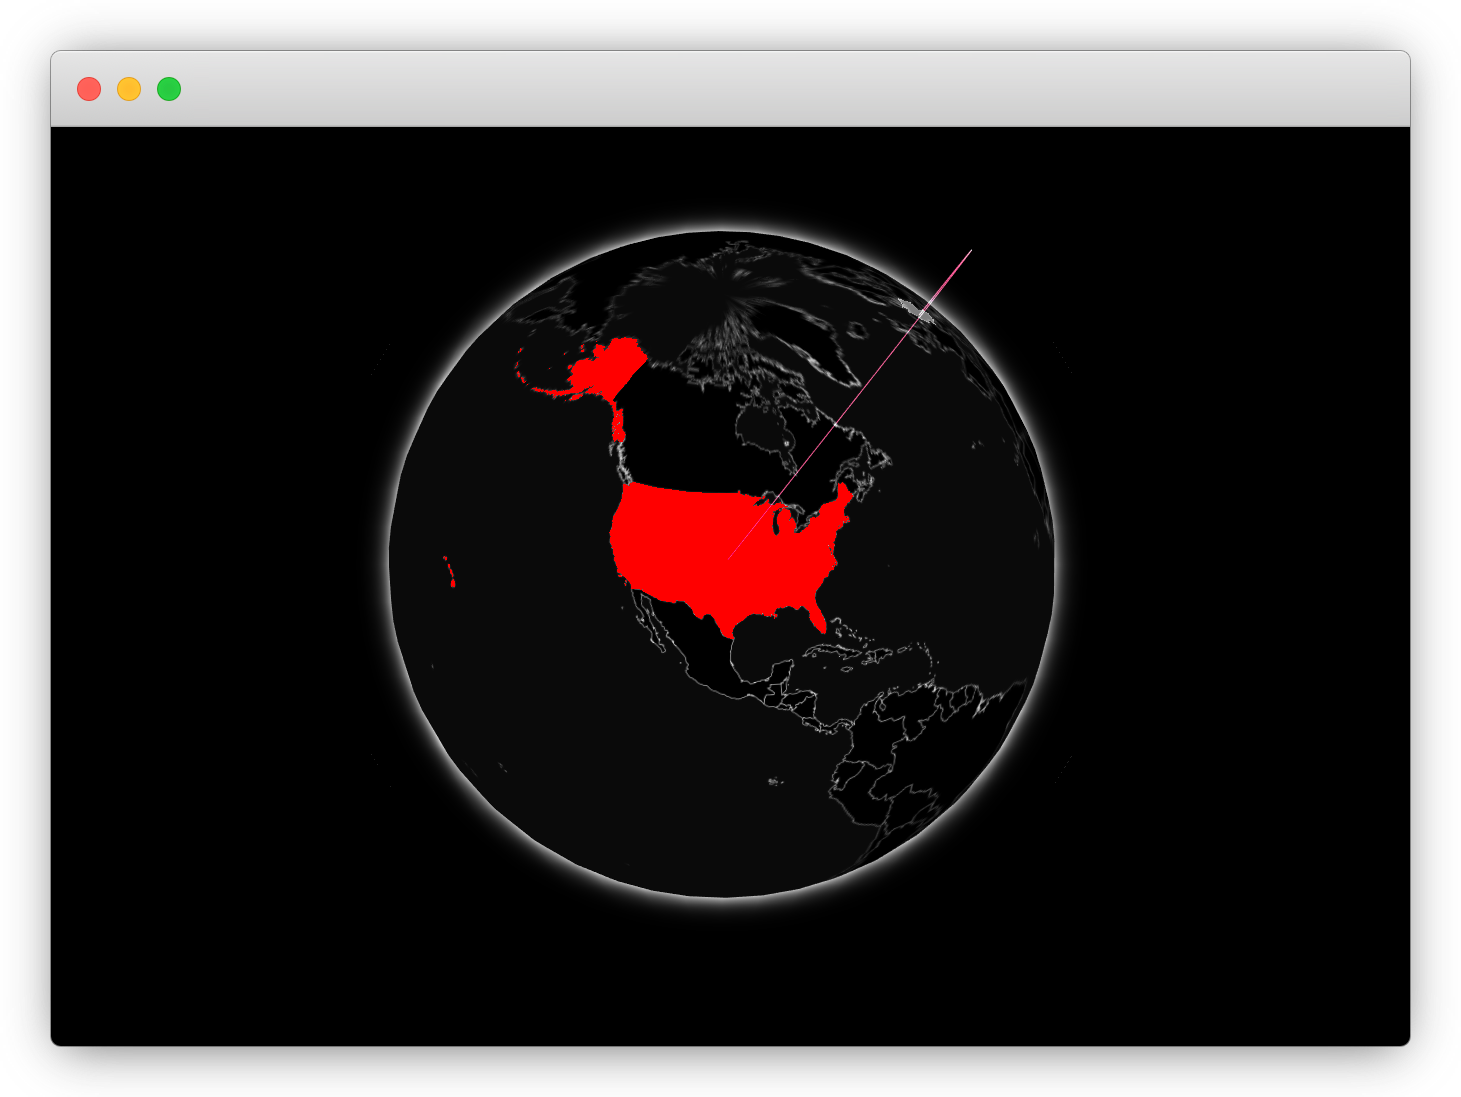
\includegraphics{images/crosstalk-three-dots.png}

\hypertarget{interface-design}{%
\section{Interface design}\label{interface-design}}

As you develop a wrapper to an external visualisation library you will have to make design choices. In building gio we more or less mirrored the JavaScript code one to one: where there is a JavaScript function to change the theme of the visualisation there is one in R, etc. This might not scale properly as more and more functions are added to the package.

As observed the gio.js library has a function named \texttt{setStyle} to change the theme of the visualisation but it has numerous others, \texttt{setSurfaceColor}, \texttt{addHalo}, \texttt{setHaloColor}, \texttt{removeHalo}, and plenty more. We might want to wrap all or some of these in a single function to provide a more convenient API to the R user.

\begin{rmdnote}
Always keep in mind the interface you make available to users of your
package.
\end{rmdnote}

You can always go beyond what the underlying library provides. For instance, the country selected by default is always China, regardless of whether the data includes that country or not. This can lead to creating underwhelming visualisations as no arcs appear. One can consider adding to the \texttt{gio} function simple heuristics to ensure that is not the case, or have the function throw a warning when the initial country is not present in the dataset.

Finally, consider R users' expectations. There are many prominent visualisation packages on CRAN already, users of the gio package will likely have used ggplot2 \citep{R-ggplot2}, plotly, or highcharter before. Though these provide somewhat different APIs they set precedents, the more the API of gio resembles those the easier it will be for new users to start using gio. However, do not let this restrict the package either, never hesitate to do differently than ggplot2 if you think it will provide a better interface to your users.

\hypertarget{excercise---ploty}{%
\chapter{Excercise - Ploty}\label{excercise---ploty}}

In this chapter we build a widget for plotly.js, or a tiny part of it; it'll allow drawing a scatter and line plot and have some additional functionalities in shiny. The aim of this chapter is to demonstrate how easily one can transfer take aways from building the gio widget to build another.

\hypertarget{discover-plotly}{%
\section{Discover Plotly}\label{discover-plotly}}

Below is a basic example from the \href{https://plotly.com/javascript/line-and-scatter/}{plotly website}. We will aim to reproduce it using htmlwidgets before improving upon it.

\begin{Shaded}
\begin{Highlighting}[]
\DataTypeTok{<!DOCTYPE }\NormalTok{html}\DataTypeTok{>}
\KeywordTok{<html}\OtherTok{ xmlns=}\StringTok{"http://www.w3.org/1999/xhtml"}\OtherTok{ lang=}\StringTok{""}\OtherTok{ xml:lang=}\StringTok{""}\KeywordTok{>}

\KeywordTok{<head>}
  \CommentTok{<!{-}{-} Import library {-}{-}>}
  \KeywordTok{<script}\OtherTok{ src=}\StringTok{"plotly{-}latest.min.js"}\KeywordTok{></script>}
\KeywordTok{</head>}

\KeywordTok{<body>}
  \CommentTok{<!{-}{-} div to hold visualisation {-}{-}>}
  \KeywordTok{<div}\OtherTok{ id=}\StringTok{"chart"}\OtherTok{ style=}\StringTok{"width:600px;height:250px;"}\KeywordTok{></div>}

  \CommentTok{<!{-}{-} Script to create visualisation {-}{-}>}
  \KeywordTok{<script>}
    \KeywordTok{var}\NormalTok{ trace1 }\OperatorTok{=} \OperatorTok{\{}
      \DataTypeTok{x}\OperatorTok{:}\NormalTok{ [}\DecValTok{1}\OperatorTok{,} \DecValTok{2}\OperatorTok{,} \DecValTok{3}\OperatorTok{,} \DecValTok{4}\NormalTok{]}\OperatorTok{,}
      \DataTypeTok{y}\OperatorTok{:}\NormalTok{ [}\DecValTok{10}\OperatorTok{,} \DecValTok{15}\OperatorTok{,} \DecValTok{13}\OperatorTok{,} \DecValTok{17}\NormalTok{]}\OperatorTok{,}
      \DataTypeTok{mode}\OperatorTok{:} \StringTok{\textquotesingle{}markers\textquotesingle{}}\OperatorTok{,}
      \DataTypeTok{type}\OperatorTok{:} \StringTok{\textquotesingle{}scatter\textquotesingle{}}
    \OperatorTok{\};}

    \KeywordTok{var}\NormalTok{ trace2 }\OperatorTok{=} \OperatorTok{\{}
      \DataTypeTok{x}\OperatorTok{:}\NormalTok{ [}\DecValTok{2}\OperatorTok{,} \DecValTok{3}\OperatorTok{,} \DecValTok{4}\OperatorTok{,} \DecValTok{5}\NormalTok{]}\OperatorTok{,}
      \DataTypeTok{y}\OperatorTok{:}\NormalTok{ [}\DecValTok{16}\OperatorTok{,} \DecValTok{5}\OperatorTok{,} \DecValTok{11}\OperatorTok{,} \DecValTok{9}\NormalTok{]}\OperatorTok{,}
      \DataTypeTok{mode}\OperatorTok{:} \StringTok{\textquotesingle{}lines\textquotesingle{}}\OperatorTok{,}
      \DataTypeTok{type}\OperatorTok{:} \StringTok{\textquotesingle{}scatter\textquotesingle{}}
    \OperatorTok{\};}

    \KeywordTok{var}\NormalTok{ data }\OperatorTok{=}\NormalTok{ [trace1}\OperatorTok{,}\NormalTok{ trace2}\OperatorTok{,}\NormalTok{ trace3]}\OperatorTok{;}

    \VariableTok{Plotly}\NormalTok{.}\AttributeTok{newPlot}\NormalTok{(}\StringTok{\textquotesingle{}chart\textquotesingle{}}\OperatorTok{,}\NormalTok{ data)}\OperatorTok{;}
\NormalTok{    )}\OperatorTok{;}
  \KeywordTok{</script>}
\KeywordTok{</body>}

\KeywordTok{</html>}
\end{Highlighting}
\end{Shaded}

The aim is to obtain an R interface resembling the already existing R package. It'll allow initialising the visualisation with the \texttt{plotly} function and add a line or scatter plot with \texttt{plot\_line} and \texttt{plot\_marker}.

\begin{Shaded}
\begin{Highlighting}[]
\KeywordTok{plotly}\NormalTok{(}\DataTypeTok{data =}\NormalTok{ cars) }\OperatorTok{\%>\%}\StringTok{ }
\StringTok{  }\KeywordTok{plot\_marker}\NormalTok{(}\DataTypeTok{x =} \StringTok{"dist"}\NormalTok{, }\DataTypeTok{y =} \StringTok{"speed"}\NormalTok{)}
\end{Highlighting}
\end{Shaded}

\hypertarget{basics-of-plotly}{%
\section{Basics of plotly}\label{basics-of-plotly}}

The story starts like all other widgets: create a package and scaffold the widget. We name the package plotlier so as to not override the local installation of the actual plotly package. We also add the magrittr pipe (\texttt{\%\textgreater{}\%}) while we're at it.

\begin{Shaded}
\begin{Highlighting}[]
\NormalTok{usethis}\OperatorTok{::}\KeywordTok{create\_package}\NormalTok{(}\StringTok{"plotlier"}\NormalTok{) }\CommentTok{\# create package}
\NormalTok{usethis}\OperatorTok{::}\KeywordTok{scaffoldWidget}\NormalTok{(}\StringTok{"plotly"}\NormalTok{) }\CommentTok{\# scaffold plotly}
\NormalTok{usethis}\OperatorTok{::}\KeywordTok{use\_pipe}\NormalTok{() }\CommentTok{\# export pipe}
\end{Highlighting}
\end{Shaded}

Then we download the dependency from the CDN, the latest version at the time of writing this is \texttt{1.54.2}, and edit the \texttt{plotly.yml} file to point to the downloaded file.

\begin{Shaded}
\begin{Highlighting}[]
\KeywordTok{dir.create}\NormalTok{(}\StringTok{"inst/htmlwidgets/plotly"}\NormalTok{, }\DataTypeTok{recursive =} \OtherTok{TRUE}\NormalTok{)}
\NormalTok{url <{-}}\StringTok{ "https://cdn.plot.ly/plotly{-}1.54.2.min.js"}
\KeywordTok{download.file}\NormalTok{(url, }\StringTok{"inst/htmlwidgets/plotly/plotly.min.js"}\NormalTok{)}
\end{Highlighting}
\end{Shaded}

\begin{Shaded}
\begin{Highlighting}[]
\FunctionTok{dependencies}\KeywordTok{:}
\AttributeTok{ }\KeywordTok{{-}}\AttributeTok{ }\FunctionTok{name}\KeywordTok{:}\AttributeTok{ plotly}
\AttributeTok{   }\FunctionTok{version}\KeywordTok{:}\AttributeTok{ }\FloatTok{1.54.2}
\AttributeTok{   }\FunctionTok{src}\KeywordTok{:}\AttributeTok{ htmlwidgets/plotly}
\AttributeTok{   }\FunctionTok{script}\KeywordTok{:}\AttributeTok{ plotly.min.js}
\end{Highlighting}
\end{Shaded}

We start by editing the \texttt{plotly} function to accept a data frame which will be stored in the \texttt{x} object. The data will not be used in this very function but will be required when adding a line or marker plot.

\begin{Shaded}
\begin{Highlighting}[]
\CommentTok{\#\textquotesingle{} @export}
\NormalTok{plotly <{-}}\StringTok{ }\ControlFlowTok{function}\NormalTok{(data, }\DataTypeTok{width =} \OtherTok{NULL}\NormalTok{, }\DataTypeTok{height =} \OtherTok{NULL}\NormalTok{, }
  \DataTypeTok{elementId =} \OtherTok{NULL}\NormalTok{) \{}

  \CommentTok{\# forward options using x}
\NormalTok{  x =}\StringTok{ }\KeywordTok{list}\NormalTok{(}
    \DataTypeTok{data =}\NormalTok{ data,}
    \DataTypeTok{options =} \KeywordTok{list}\NormalTok{()}
\NormalTok{  )}

  \CommentTok{\# create widget}
\NormalTok{  htmlwidgets}\OperatorTok{::}\KeywordTok{createWidget}\NormalTok{(}
    \DataTypeTok{name =} \StringTok{\textquotesingle{}plotly\textquotesingle{}}\NormalTok{,}
\NormalTok{    x,}
    \DataTypeTok{width =}\NormalTok{ width,}
    \DataTypeTok{height =}\NormalTok{ height,}
    \DataTypeTok{package =} \StringTok{\textquotesingle{}plotlier\textquotesingle{}}\NormalTok{,}
    \DataTypeTok{elementId =}\NormalTok{ elementId}
\NormalTok{  )}
\NormalTok{\}}
\end{Highlighting}
\end{Shaded}

The JavaScript would look like the code below. It's actually much easier than what had to be written for gio.js as the function to generate a new plot accepts 1) the id of the \texttt{\textless{}div\textgreater{}} where the plot should be created and 2) a JSON object of options (containing the data) which describes the plot.

\begin{Shaded}
\begin{Highlighting}[]
\VariableTok{HTMLWidgets}\NormalTok{.}\AttributeTok{widget}\NormalTok{(}\OperatorTok{\{}

  \DataTypeTok{name}\OperatorTok{:} \StringTok{\textquotesingle{}plotly\textquotesingle{}}\OperatorTok{,}

  \DataTypeTok{type}\OperatorTok{:} \StringTok{\textquotesingle{}output\textquotesingle{}}\OperatorTok{,}

  \DataTypeTok{factory}\OperatorTok{:} \KeywordTok{function}\NormalTok{(el}\OperatorTok{,}\NormalTok{ width}\OperatorTok{,}\NormalTok{ height) }\OperatorTok{\{}

    \ControlFlowTok{return} \OperatorTok{\{}

      \DataTypeTok{renderValue}\OperatorTok{:} \KeywordTok{function}\NormalTok{(x) }\OperatorTok{\{}

        \CommentTok{// create plot}
        \VariableTok{Plotly}\NormalTok{.}\AttributeTok{newPlot}\NormalTok{(}\VariableTok{el}\NormalTok{.}\AttributeTok{id}\OperatorTok{,} \VariableTok{x}\NormalTok{.}\AttributeTok{options}\NormalTok{)}\OperatorTok{;}

      \OperatorTok{\},}

      \DataTypeTok{resize}\OperatorTok{:} \KeywordTok{function}\NormalTok{(width}\OperatorTok{,}\NormalTok{ height) }\OperatorTok{\{}

        \CommentTok{// }\AlertTok{TODO}\CommentTok{: code to re{-}render the widget with a new size}

      \OperatorTok{\}}

    \OperatorTok{\};}
  \OperatorTok{\}}
\OperatorTok{\}}\NormalTok{)}\OperatorTok{;}
\end{Highlighting}
\end{Shaded}

Then it's a matter of reproducing the JSON that defines what plotly describes as a ``trace'' and what more or less corresponds to a ``geom'' in ggplot2. A trace for a scatter plot is defined with the JSON below, which we can read in R to understand the shape of the list to reproduce.

\begin{Shaded}
\begin{Highlighting}[]
\NormalTok{jsonlite}\OperatorTok{::}\KeywordTok{fromJSON}\NormalTok{(}\StringTok{\textquotesingle{}\{}
\StringTok{	"x": [1, 2, 3, 4],}
\StringTok{	"y": [10, 15, 13, 17],}
\StringTok{	"mode": "markers",}
\StringTok{	"type": "scatter"}
\StringTok{\}\textquotesingle{}}\NormalTok{)}
\end{Highlighting}
\end{Shaded}

\begin{verbatim}
## $x
## [1] 1 2 3 4
## 
## $y
## [1] 10 15 13 17
## 
## $mode
## [1] "markers"
## 
## $type
## [1] "scatter"
\end{verbatim}

We can then create a function that takes the name of the x and y columns to fetch from the data which is accessible from the plotly object with \texttt{p\$x\$data}

\begin{Shaded}
\begin{Highlighting}[]
\CommentTok{\#\textquotesingle{} @export}
\NormalTok{plot\_marker <{-}}\StringTok{ }\ControlFlowTok{function}\NormalTok{(p, x, y)\{}
\NormalTok{  layer <{-}}\StringTok{ }\KeywordTok{list}\NormalTok{(}
    \DataTypeTok{x =}\NormalTok{ p}\OperatorTok{$}\NormalTok{x}\OperatorTok{$}\NormalTok{data[[x]],}
    \DataTypeTok{y =}\NormalTok{ p}\OperatorTok{$}\NormalTok{x}\OperatorTok{$}\NormalTok{data[[y]],}
    \DataTypeTok{type =} \StringTok{"scatter"}\NormalTok{,}
    \DataTypeTok{mode =} \StringTok{"markers"}
\NormalTok{  )}

\NormalTok{  p}\OperatorTok{$}\NormalTok{x}\OperatorTok{$}\NormalTok{options <{-}}\StringTok{ }\KeywordTok{append}\NormalTok{(p}\OperatorTok{$}\NormalTok{x}\OperatorTok{$}\NormalTok{options, }\KeywordTok{list}\NormalTok{(layer))}
  \KeywordTok{return}\NormalTok{(p)}
\NormalTok{\}}
\end{Highlighting}
\end{Shaded}

At this stage the functions \texttt{devtools::document} and \texttt{devtools::load\_all} can be run so the package can be tested.

\begin{Shaded}
\begin{Highlighting}[]
\KeywordTok{library}\NormalTok{(plotlier)}

\KeywordTok{plotly}\NormalTok{(cars) }\OperatorTok{\%>\%}\StringTok{ }
\StringTok{  }\KeywordTok{plot\_marker}\NormalTok{(}\StringTok{"dist"}\NormalTok{, }\StringTok{"speed"}\NormalTok{)}
\end{Highlighting}
\end{Shaded}

\begin{figure}
\centering
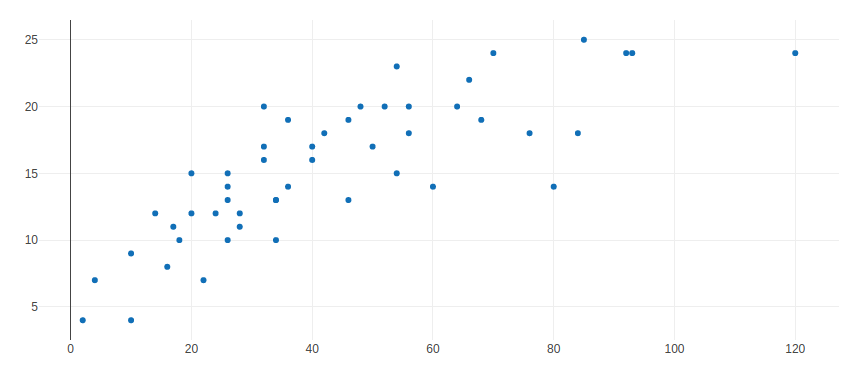
\includegraphics{images/plotlier-scatter.png}
\caption{Plotlier Scatter plot}
\end{figure}

\hypertarget{javascript-to-r}{%
\section{JavaScript to R}\label{javascript-to-r}}

We can now look up plotly's documentation on \href{https://plotly.com/javascript/plotlyjs-events/}{callback} to send data to the R server when a point is clicked.

\begin{Shaded}
\begin{Highlighting}[]
\NormalTok{...}
\NormalTok{renderValue}\OperatorTok{:} \KeywordTok{function}\NormalTok{(x) }\OperatorTok{\{}

  \VariableTok{Plotly}\NormalTok{.}\AttributeTok{newPlot}\NormalTok{(}\VariableTok{el}\NormalTok{.}\AttributeTok{id}\OperatorTok{,} \VariableTok{x}\NormalTok{.}\AttributeTok{options}\NormalTok{)}\OperatorTok{;}

  \VariableTok{plot}\NormalTok{.}\AttributeTok{on}\NormalTok{(}\StringTok{\textquotesingle{}plotly\_click\textquotesingle{}}\OperatorTok{,} \KeywordTok{function}\NormalTok{(data)}\OperatorTok{\{}
    \KeywordTok{var}\NormalTok{ coords }\OperatorTok{=}\NormalTok{ [}\VariableTok{data}\NormalTok{.}\AttributeTok{points}\NormalTok{[}\DecValTok{0}\NormalTok{].}\AttributeTok{x}\OperatorTok{,} \VariableTok{data}\NormalTok{.}\AttributeTok{points}\NormalTok{[}\DecValTok{0}\NormalTok{].}\AttributeTok{y}\NormalTok{]}\OperatorTok{;}
    \VariableTok{Shiny}\NormalTok{.}\AttributeTok{setInputValue}\NormalTok{(}\VariableTok{el}\NormalTok{.}\AttributeTok{id} \OperatorTok{+} \StringTok{\textquotesingle{}\_clicked\textquotesingle{}}\OperatorTok{,}\NormalTok{ coords)}\OperatorTok{;}
  \OperatorTok{\}}\NormalTok{)}\OperatorTok{;}

\OperatorTok{\}}
\NormalTok{...}
\end{Highlighting}
\end{Shaded}

Finally, we load the package's functions using devtools to test the input.

\begin{Shaded}
\begin{Highlighting}[]
\KeywordTok{library}\NormalTok{(shiny)}
\KeywordTok{library}\NormalTok{(plotlier)}

\NormalTok{ui <{-}}\StringTok{ }\KeywordTok{fluidPage}\NormalTok{(}
  \KeywordTok{plotlyOutput}\NormalTok{(}\StringTok{"plot"}\NormalTok{),}
  \KeywordTok{verbatimTextOutput}\NormalTok{(}\StringTok{"clicked"}\NormalTok{)}
\NormalTok{)}

\NormalTok{server <{-}}\StringTok{ }\ControlFlowTok{function}\NormalTok{(input, output)\{}

\NormalTok{  output}\OperatorTok{$}\NormalTok{plot <{-}}\StringTok{ }\KeywordTok{renderPlotly}\NormalTok{(\{}
    \KeywordTok{plotly}\NormalTok{(cars) }\OperatorTok{\%>\%}\StringTok{ }
\StringTok{      }\KeywordTok{plot\_marker}\NormalTok{(}\StringTok{"dist"}\NormalTok{, }\StringTok{"speed"}\NormalTok{)}
\NormalTok{  \})}

\NormalTok{  output}\OperatorTok{$}\NormalTok{clicked <{-}}\StringTok{ }\KeywordTok{renderPrint}\NormalTok{(\{}
    \KeywordTok{print}\NormalTok{(input}\OperatorTok{$}\NormalTok{plot\_clicked)}
\NormalTok{  \})}

\NormalTok{\}}

\KeywordTok{shinyApp}\NormalTok{(ui, server)}
\end{Highlighting}
\end{Shaded}

\hypertarget{r-to-javascript}{%
\section{R to JavaScript}\label{r-to-javascript}}

Here we implement an example of passing data from R to JavaScript, name the JavaScript \texttt{addTraces} function which allows dynamically adding traces to the chart without redrawing it in its entirety.

The JavaScript \texttt{addTraces} function takes the id of the chart to add the trace to and a JSON object that defines the trace.

\begin{Shaded}
\begin{Highlighting}[]
\CommentTok{// addTraces example}
\VariableTok{Plotly}\NormalTok{.}\AttributeTok{addTraces}\NormalTok{(}\StringTok{\textquotesingle{}plot\textquotesingle{}}\OperatorTok{,} \OperatorTok{\{}\DataTypeTok{y}\OperatorTok{:}\NormalTok{ [}\DecValTok{2}\OperatorTok{,}\DecValTok{1}\OperatorTok{,}\DecValTok{2}\NormalTok{]}\OperatorTok{\}}\NormalTok{)}\OperatorTok{;}
\end{Highlighting}
\end{Shaded}

We start, as done previously, by defining a ``proxy,'' a function that returns an object containing information necessary to add traces to the chart, namely the \texttt{id} of the chart to apply to and the \texttt{session} object which will be used to send the data.

\begin{Shaded}
\begin{Highlighting}[]
\CommentTok{\#\textquotesingle{} @export}
\NormalTok{plotlyProxy <{-}}\StringTok{ }\ControlFlowTok{function}\NormalTok{(id, }
  \DataTypeTok{session =}\NormalTok{ shiny}\OperatorTok{::}\KeywordTok{getDefaultReactiveDomain}\NormalTok{())\{}
  \KeywordTok{list}\NormalTok{(}
    \DataTypeTok{id =}\NormalTok{ id,}
    \DataTypeTok{session =}\NormalTok{ session}
\NormalTok{  )}
\NormalTok{\}}
\end{Highlighting}
\end{Shaded}

We then create a function that creates the trace and sends that data, together with the plot \texttt{id}, to JavaScript as a message of type ``add-traces.''

\begin{Shaded}
\begin{Highlighting}[]
\CommentTok{\#\textquotesingle{} @export}
\NormalTok{plot\_add\_marker <{-}}\StringTok{ }\ControlFlowTok{function}\NormalTok{(proxy, data, x, y)\{}
\NormalTok{  data <{-}}\StringTok{ }\KeywordTok{list}\NormalTok{(}
    \DataTypeTok{x =}\NormalTok{ data[[x]],}
    \DataTypeTok{y =}\NormalTok{ data[[y]],}
    \DataTypeTok{type =} \StringTok{"scatter"}\NormalTok{,}
    \DataTypeTok{mode =} \StringTok{"markers"}
\NormalTok{  )}

\NormalTok{  msg <{-}}\StringTok{ }\KeywordTok{list}\NormalTok{(}\DataTypeTok{id =}\NormalTok{ proxy}\OperatorTok{$}\NormalTok{id, }\DataTypeTok{data =}\NormalTok{ data)}
\NormalTok{  proxy}\OperatorTok{$}\NormalTok{session}\OperatorTok{$}\KeywordTok{sendCustomMessage}\NormalTok{(}\StringTok{"add{-}traces"}\NormalTok{, msg)}
  \KeywordTok{return}\NormalTok{(proxy)}
\NormalTok{\}}
\end{Highlighting}
\end{Shaded}

Finally, we add a message handler to handle the data sent to \texttt{add-traces} and use the JavaScript method \texttt{addTraces} to add a trace to the plot.

\begin{Shaded}
\begin{Highlighting}[]
\ControlFlowTok{if}\NormalTok{(}\VariableTok{HTMLWidgets}\NormalTok{.}\AttributeTok{shinyMode}\NormalTok{)}\OperatorTok{\{}

  \VariableTok{Shiny}\NormalTok{.}\AttributeTok{addCustomMessageHandler}\NormalTok{(}
\NormalTok{    type }\OperatorTok{=} \StringTok{\textquotesingle{}add{-}traces\textquotesingle{}}\OperatorTok{,} \KeywordTok{function}\NormalTok{(msg)}\OperatorTok{\{}
      \VariableTok{Plotly}\NormalTok{.}\AttributeTok{addTraces}\NormalTok{(}\VariableTok{msg}\NormalTok{.}\AttributeTok{id}\OperatorTok{,} \VariableTok{msg}\NormalTok{.}\AttributeTok{data}\NormalTok{)}\OperatorTok{;}
    \OperatorTok{\}}
\NormalTok{  )}

\OperatorTok{\}}
\end{Highlighting}
\end{Shaded}

After installing the package, one can use the new proxy function in a shiny application, below we provide a button that adds a trace of random data to the chart.

\begin{Shaded}
\begin{Highlighting}[]
\KeywordTok{library}\NormalTok{(shiny)}
\KeywordTok{library}\NormalTok{(plotlier)}

\NormalTok{df <{-}}\StringTok{ }\KeywordTok{data.frame}\NormalTok{(}\DataTypeTok{x =} \DecValTok{1}\OperatorTok{:}\DecValTok{10}\NormalTok{, }\DataTypeTok{y =} \KeywordTok{runif}\NormalTok{(}\DecValTok{10}\NormalTok{))}

\NormalTok{ui <{-}}\StringTok{ }\KeywordTok{fluidPage}\NormalTok{(}
  \KeywordTok{actionButton}\NormalTok{(}\StringTok{"add"}\NormalTok{, }\StringTok{"Add random trace"}\NormalTok{),}
  \KeywordTok{plotlyOutput}\NormalTok{(}\StringTok{"plot"}\NormalTok{)}
\NormalTok{)}

\NormalTok{server <{-}}\StringTok{ }\ControlFlowTok{function}\NormalTok{(input, output)\{}

\NormalTok{  output}\OperatorTok{$}\NormalTok{plot <{-}}\StringTok{ }\KeywordTok{renderPlotly}\NormalTok{(\{}
\NormalTok{    df }\OperatorTok{\%>\%}\StringTok{ }
\StringTok{      }\KeywordTok{plotly}\NormalTok{() }\OperatorTok{\%>\%}\StringTok{ }
\StringTok{      }\KeywordTok{plot\_line}\NormalTok{(}\StringTok{"x"}\NormalTok{, }\StringTok{"y"}\NormalTok{)}
\NormalTok{  \})}

\NormalTok{  proxy <{-}}\StringTok{ }\KeywordTok{plotlyProxy}\NormalTok{(}\StringTok{"plot"}\NormalTok{)}

  \KeywordTok{observeEvent}\NormalTok{(input}\OperatorTok{$}\NormalTok{add, \{}
\NormalTok{    random <{-}}\StringTok{ }\KeywordTok{data.frame}\NormalTok{(}\DataTypeTok{x =} \KeywordTok{runif}\NormalTok{(}\DecValTok{10}\NormalTok{, }\DecValTok{1}\NormalTok{, }\DecValTok{10}\NormalTok{), }\DataTypeTok{y =} \KeywordTok{runif}\NormalTok{(}\DecValTok{10}\NormalTok{))}
    
    \KeywordTok{plot\_add\_marker}\NormalTok{(}
\NormalTok{      proxy,}
\NormalTok{      random,}
      \StringTok{"x"}\NormalTok{, }\StringTok{"y"}
\NormalTok{    )}
\NormalTok{  \})}

\NormalTok{\}}

\KeywordTok{shinyApp}\NormalTok{(ui, server)}
\end{Highlighting}
\end{Shaded}

\begin{figure}
\centering
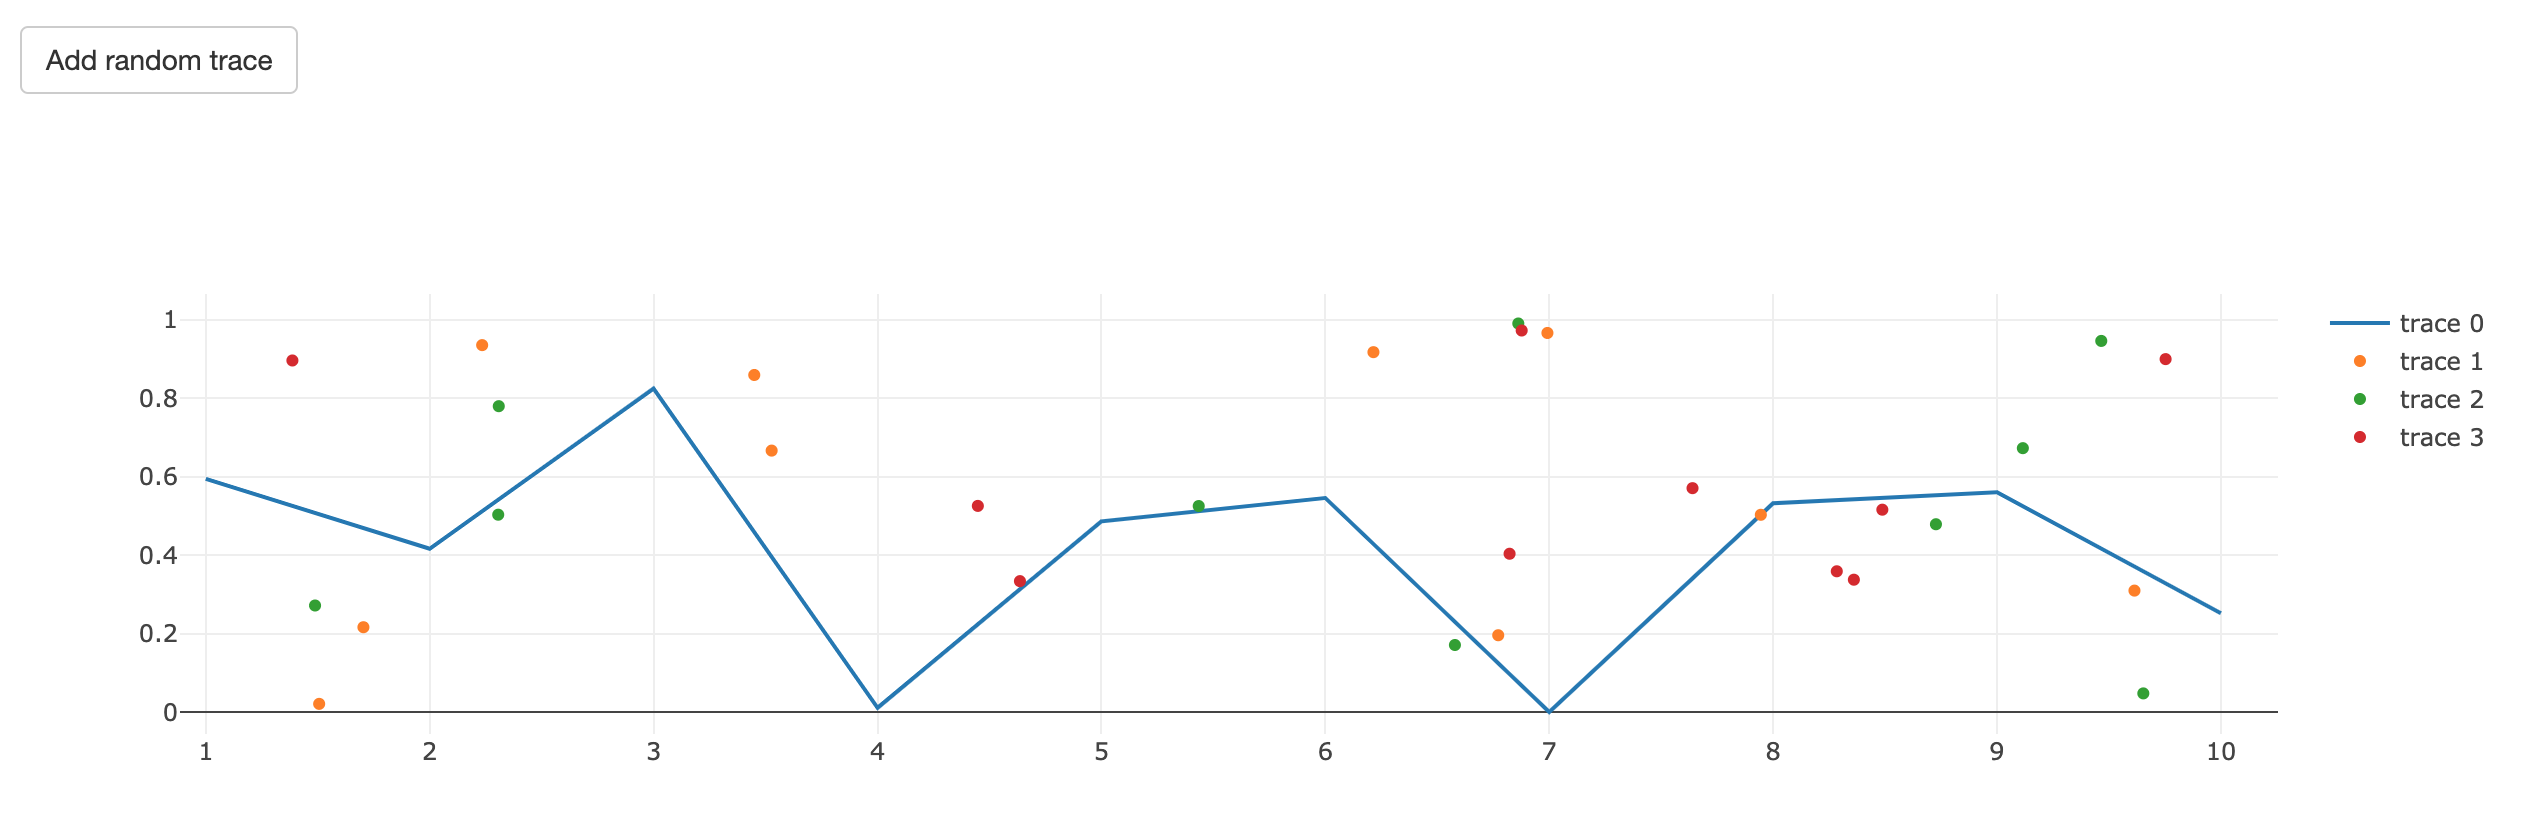
\includegraphics{images/plotlier-add.png}
\caption{Plotly with dynamic traces}
\end{figure}

\hypertarget{size-resize}{%
\section{Size \& Resize}\label{size-resize}}

At this stage the plotlier package does yet provide responsive visualisation: resizing the screen does not resize the visualisation. In order to ensure that it is we have to define a default width that is not defined in pixel but percentage (such as 100\%) and implement the resize method.

As mentioned in a previous chapter, the default size can be changed with the \texttt{sizingPolicy} function, below we set it to \texttt{100\%}.

\begin{Shaded}
\begin{Highlighting}[]
\CommentTok{\# create widget}
\NormalTok{htmlwidgets}\OperatorTok{::}\KeywordTok{createWidget}\NormalTok{(}
  \DataTypeTok{name =} \StringTok{\textquotesingle{}plotly\textquotesingle{}}\NormalTok{,}
\NormalTok{  x,}
  \DataTypeTok{width =}\NormalTok{ width,}
  \DataTypeTok{height =}\NormalTok{ height,}
  \DataTypeTok{package =} \StringTok{\textquotesingle{}plotlier\textquotesingle{}}\NormalTok{,}
  \DataTypeTok{elementId =}\NormalTok{ elementId,}
  \DataTypeTok{preRenderHook =}\NormalTok{ render\_plotlier,}
  \DataTypeTok{sizingPolicy =} \KeywordTok{sizingPolicy}\NormalTok{(}
    \DataTypeTok{defaultWidth =} \StringTok{"100\%"}
\NormalTok{  )}
\NormalTok{)}
\end{Highlighting}
\end{Shaded}

Next we can use the plotly function \texttt{relayout} to resize the visualisation when the size of its container changes.

\begin{Shaded}
\begin{Highlighting}[]
\NormalTok{resize}\OperatorTok{:} \KeywordTok{function}\NormalTok{(width}\OperatorTok{,}\NormalTok{ height) }\OperatorTok{\{}
  \VariableTok{Plotly}\NormalTok{.}\AttributeTok{relayout}\NormalTok{(}\VariableTok{el}\NormalTok{.}\AttributeTok{id}\OperatorTok{,} \OperatorTok{\{}\DataTypeTok{width}\OperatorTok{:}\NormalTok{ width}\OperatorTok{,} \DataTypeTok{height}\OperatorTok{:}\NormalTok{ height}\OperatorTok{\}}\NormalTok{)}\OperatorTok{;}
\OperatorTok{\}}
\end{Highlighting}
\end{Shaded}

One can test this by resizing the browser or RStudio viewer window.

\begin{Shaded}
\begin{Highlighting}[]
\KeywordTok{plotly}\NormalTok{(cars) }\OperatorTok{\%>\%}\StringTok{  }
\StringTok{      }\KeywordTok{plot\_marker}\NormalTok{(}\StringTok{"dist"}\NormalTok{, }\StringTok{"speed"}\NormalTok{)}
\end{Highlighting}
\end{Shaded}

\begin{figure}
\centering
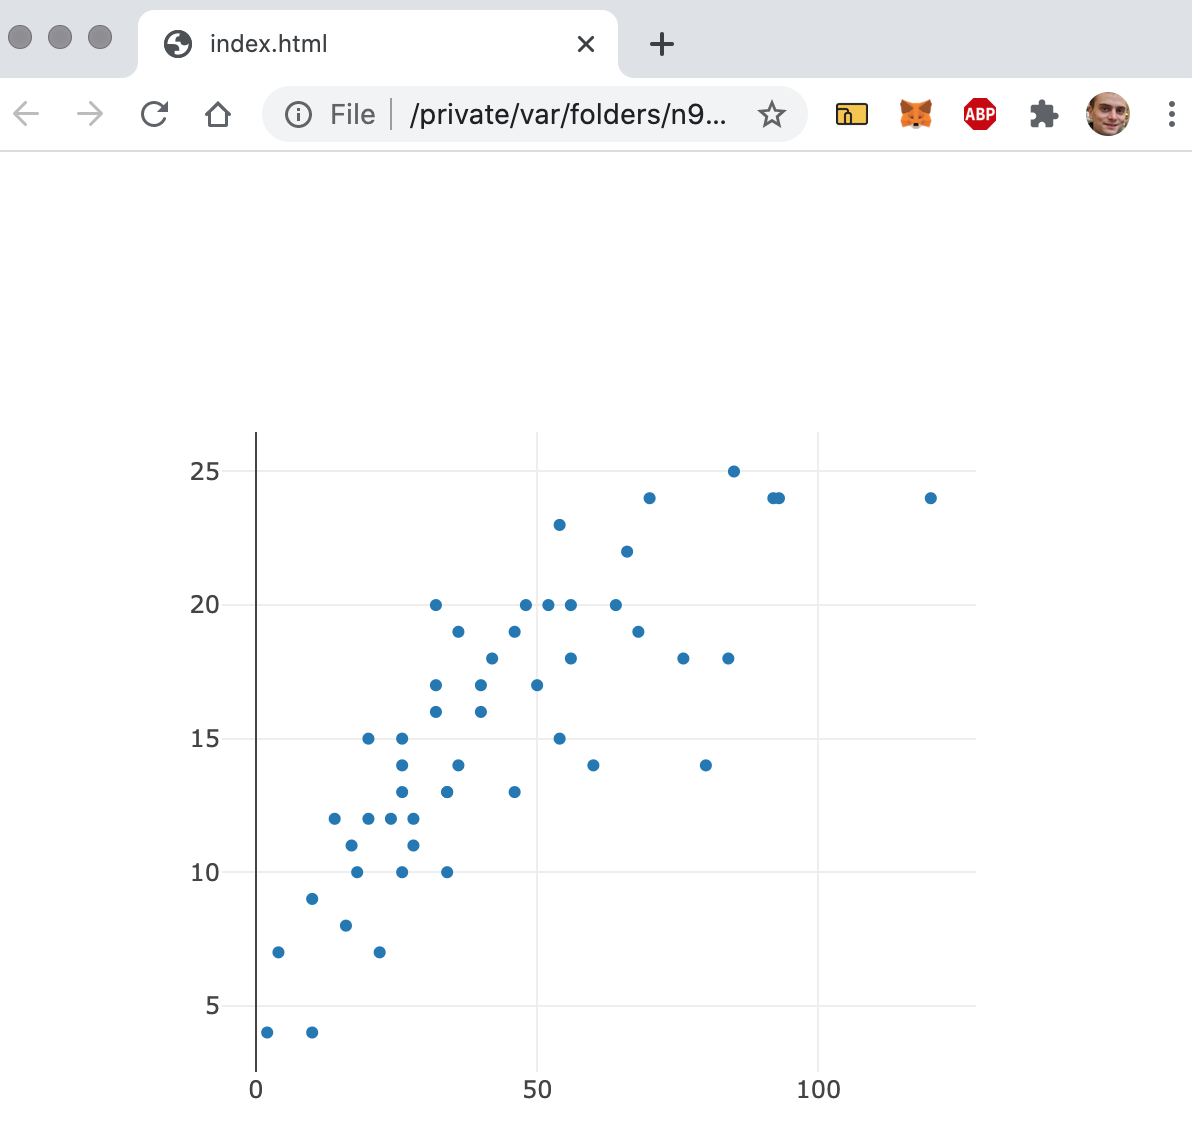
\includegraphics{images/plotlier-responsive.png}
\caption{Responsive plotly output}
\end{figure}

\hypertarget{performance-security}{%
\section{Performance \& Security}\label{performance-security}}

The package stores the data passed to the \texttt{plotly} function in the widget object, however, as explained in a previous chapter this is insecure and a drain on performances. First, this data serialised to JSON but not used in JavaScript and thus leads to unnecessary computations. Second, this data is visible on the resulting visualisation which may cause security concerns given the user may not deliberately use all the data in the visualisation. This can be remedied to by use the \texttt{preRenderHook}.

\begin{Shaded}
\begin{Highlighting}[]
\NormalTok{render\_plotlier <{-}}\StringTok{ }\ControlFlowTok{function}\NormalTok{(p)\{}
\NormalTok{  p}\OperatorTok{$}\NormalTok{x}\OperatorTok{$}\NormalTok{data <{-}}\StringTok{ }\OtherTok{NULL}
  \KeywordTok{return}\NormalTok{(p)}
\NormalTok{\}}
\end{Highlighting}
\end{Shaded}

The function define above can then be used in the \texttt{htmlwidgets::createWidget} function so it is run just before the visualisation renders.

\begin{Shaded}
\begin{Highlighting}[]
\NormalTok{htmlwidgets}\OperatorTok{::}\KeywordTok{createWidget}\NormalTok{(}
  \DataTypeTok{name =} \StringTok{\textquotesingle{}plotly\textquotesingle{}}\NormalTok{,}
\NormalTok{  x,}
  \DataTypeTok{width =}\NormalTok{ width,}
  \DataTypeTok{height =}\NormalTok{ height,}
  \DataTypeTok{package =} \StringTok{\textquotesingle{}plotlier\textquotesingle{}}\NormalTok{,}
  \DataTypeTok{elementId =}\NormalTok{ elementId,}
  \DataTypeTok{preRenderHook =}\NormalTok{ render\_plotlier}
\NormalTok{)}
\end{Highlighting}
\end{Shaded}

\hypertarget{part-web-development-with-shiny}{%
\part{Web Development with Shiny}\label{part-web-development-with-shiny}}

\hypertarget{introduction-to-shiny}{%
\chapter{Introduction to shiny}\label{introduction-to-shiny}}

Shiny is the web framework of choice for the R programming language. Since JavaScript and Shiny both run in web browsers it follows that they can run alongside one another as one can include JavaScript in such applications. Yet, often disregarded is the ability for Shiny's R server to communicate to the front-end and vice versa. This collection of chapters aims to show precisely how this works. In this first part, we brush up on the essentials so we understand how to include JavaScript in shiny applications.

Then again, the goal is not to write a lot of convoluted JavaScript, on the contrary, with little knowledge of the language the aim is to write as little as possible but demonstrate to the reader that it is often enough to greatly improve the user experience of shiny applications.

\hypertarget{websocket}{%
\section{Websocket}\label{websocket}}

Shiny applications have two components the user interface (UI) and the server function. These two components communicate via a websocket: a persistent connection that allows passing messages between the server and clients connecting to it. In the R server this connection is managed by shiny using the httpuv \citep{R-httpuv} and websocket \citep{R-websocket} packages, while in clients connecting to the server this connection is managed with JavaScript.

\begin{center}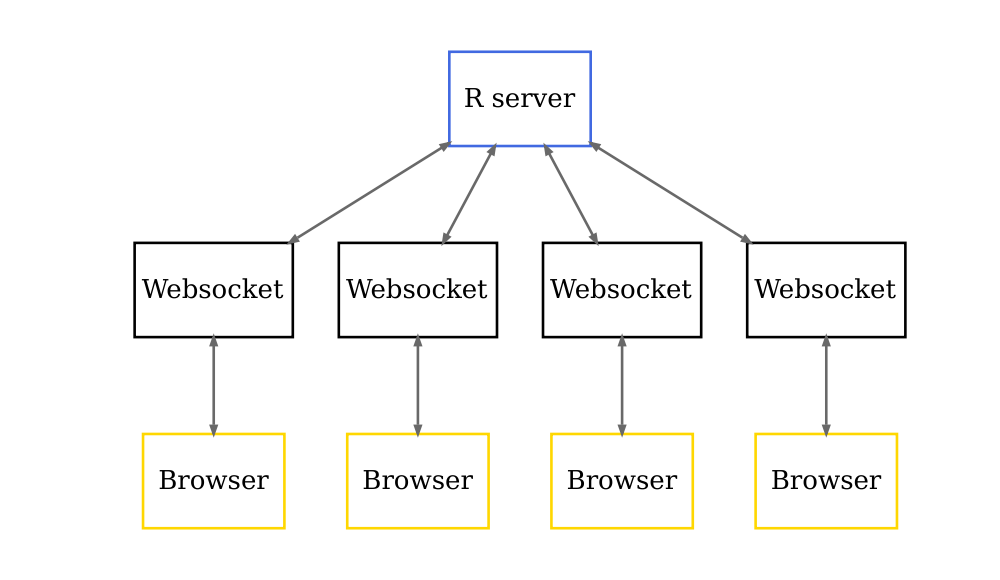
\includegraphics[width=1\linewidth]{bookdown_files/figure-latex/unnamed-chunk-45-1} \end{center}

With that in mind we can put together a shiny applications which though simple exploits bi-directional communication. The application takes a text input, sends the value of the input to the R server which sends it back to the UI.

\begin{Shaded}
\begin{Highlighting}[]
\KeywordTok{library}\NormalTok{(shiny)}

\NormalTok{ui <{-}}\StringTok{ }\KeywordTok{fluidPage}\NormalTok{(}
  \KeywordTok{textInput}\NormalTok{(}\StringTok{"nameInput"}\NormalTok{, }\StringTok{"Your name"}\NormalTok{),}
  \KeywordTok{textOutput}\NormalTok{(}\StringTok{"nameOutput"}\NormalTok{)}
\NormalTok{)}

\NormalTok{server <{-}}\StringTok{ }\ControlFlowTok{function}\NormalTok{(input, output) \{}
\NormalTok{  output}\OperatorTok{$}\NormalTok{nameOutput <{-}}\StringTok{ }\KeywordTok{renderText}\NormalTok{(\{}
\NormalTok{    input}\OperatorTok{$}\NormalTok{nameInput}
\NormalTok{  \})}
\NormalTok{\}}

\KeywordTok{shinyApp}\NormalTok{(ui, server)}
\end{Highlighting}
\end{Shaded}

Drawing a diagram of the communication between the UI and the server reveals that thought this is a simple application a lot is happening.

\begin{Shaded}
\begin{Highlighting}[]
\NormalTok{DiagrammeR}\OperatorTok{::}\KeywordTok{grViz}\NormalTok{(}\StringTok{"}
\StringTok{digraph \{}
\StringTok{  graph[rankdir=LR]}
\StringTok{  node[shape=record]}

\StringTok{  subgraph cluster\_0 \{}
\StringTok{    textInput}
\StringTok{    textOutput}
\StringTok{    label=\textquotesingle{}User Interface\textquotesingle{}}
\StringTok{    color=gold}
\StringTok{  \}}

\StringTok{  subgraph cluster\_1 \{}
\StringTok{    \textquotesingle{}input list\textquotesingle{}}
\StringTok{    renderOutput}
\StringTok{    label=\textquotesingle{}R server\textquotesingle{}}
\StringTok{    color=royalBlue}
\StringTok{  \}}

\StringTok{  textInput {-}> \textquotesingle{}input list\textquotesingle{} [xlabel=websocket]}
\StringTok{  \textquotesingle{}input list\textquotesingle{} {-}> renderOutput}
\StringTok{  renderOutput {-}> textOutput [label=websocket]}
\StringTok{\}}
\StringTok{"}\NormalTok{)}
\end{Highlighting}
\end{Shaded}

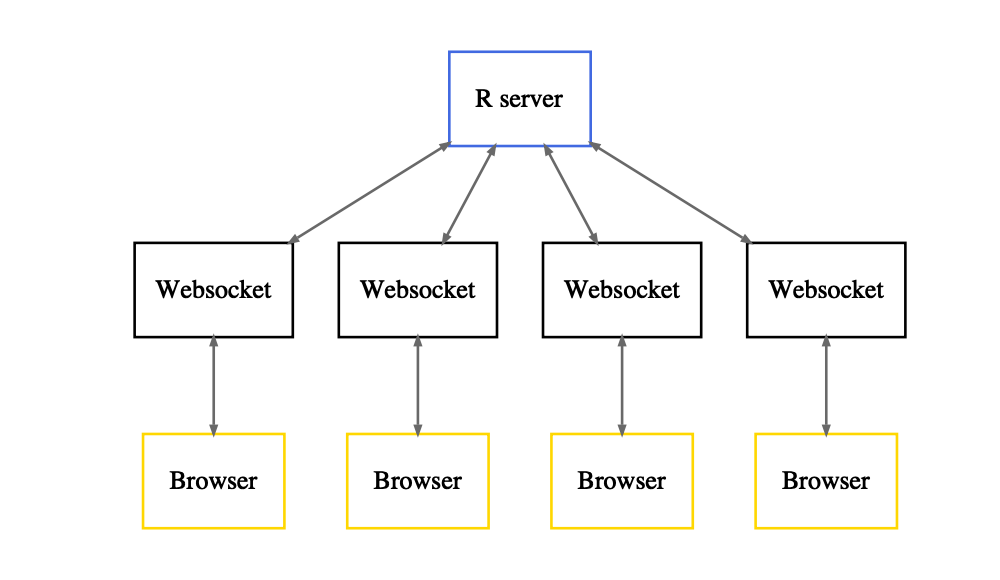
\includegraphics{bookdown_files/figure-latex/unnamed-chunk-46-1.png}

Communicating between the R server and the user interface requires JavaScript and thus makes us a reasonable chunk of this part of the book on web development with shiny.

\hypertarget{static-files}{%
\section{Static files}\label{static-files}}

In order to introduce JavaScript to shiny applications one must understand static files and how they work with the framework. Static files are files that are downloaded by the clients, in this case web browsers accessing shiny applications, as-is, these generally include images, CSS (\texttt{.css}), and JavaScript (\texttt{.js}).

If you are familiar with R packages it enables development, static files are to shiny applications what the ``inst'' directory is to an R package, those files are installed as-is and do not require further processing as opposed to the ``src'' folder which contains files that need compiling for instance.

There are numerous functions to launch a shiny application locally; the two most used probably are \texttt{shinyApp} and \texttt{runApp}. The RStudio IDE comes with a convenient ``Run'' button when writing a shiny application, which when clicked actually uses the function \texttt{shiny::runApp} in the background, this function looks for said static files in the \texttt{www} directory and makes them available at the same path (\texttt{/www}). If you are building your applications outside of RStudio, you should either also use \texttt{shiny::runApp} or specify the directory which then allows using \texttt{shiny::shinyApp}. Note that this only applies locally, shiny server (community and pro) as well as \href{https://www.shinyapps.io/}{shinyapps.io} use the same defaults as the RStudio IDE and \texttt{shiny::runApp}.

In order to ensure the code in this book can run regardless of the reader's machine or editor, the asset directory is always specified explicitly. This is probably advised to steer clear of the potential headaches as, unlike the default, it'll work regardless of the environment. If you are using \href{https://thinkr-open.github.io/golem/}{golem} \citep{R-golem} to develop your application then you should not worry about this as it specifies the directory internally.

Below we build a basic shiny application, however, before we define the ui and server we use the \texttt{shiny::addResourcePath} function to specify the location of the directory of static files that will be served by the server and thus accessible by the client. This function takes two arguments, first the \texttt{prefix}, which is the path (URL) at which the assets will be available, second the path to the directory of static assets.

We thus create the ``assets'' directory and a JavaScript file called \texttt{script.js} within it.

\begin{Shaded}
\begin{Highlighting}[]
\CommentTok{\# run from root of app (where app.R is located)}
\KeywordTok{dir.create}\NormalTok{(}\StringTok{"assets"}\NormalTok{)}
\KeywordTok{writeLines}\NormalTok{(}\StringTok{"console.log(\textquotesingle{}Hello JS!\textquotesingle{});"}\NormalTok{, }\DataTypeTok{con =} \StringTok{"assets/script.js"}\NormalTok{)}
\end{Highlighting}
\end{Shaded}

We can now use the \texttt{shiny::addResourcePath} to point to this directory. Generally the same name for the directory of static assets and prefix is used so as to avoid confusion, below we name them differently in order for the reader to clearly distinguish which is which.

\begin{Shaded}
\begin{Highlighting}[]
\CommentTok{\# app.R}
\KeywordTok{library}\NormalTok{(shiny)}

\CommentTok{\# serve the files}
\KeywordTok{addResourcePath}\NormalTok{(}
  \CommentTok{\# will be accessible at /files}
  \DataTypeTok{prefix =} \StringTok{"files"}\NormalTok{, }
  \CommentTok{\# path to the assets directory}
  \DataTypeTok{directoryPath =} \StringTok{"assets"}
\NormalTok{)}

\NormalTok{ui <{-}}\StringTok{ }\KeywordTok{fluidPage}\NormalTok{(}
  \KeywordTok{h1}\NormalTok{(}\StringTok{"R and JavaScript"}\NormalTok{)}
\NormalTok{)}

\NormalTok{server <{-}}\StringTok{ }\ControlFlowTok{function}\NormalTok{(input, output)\{\}}

\KeywordTok{shinyApp}\NormalTok{(ui, server)}
\end{Highlighting}
\end{Shaded}

If you then run the application and open it at the \texttt{/files/script.js} path (e.g.: \texttt{127.0.0.1:3000/files/script.js}) you should see the content of the JavaScript file (\texttt{console.log(\textquotesingle{}Hello\ JS!\textquotesingle{})}), commenting the \texttt{addResourcePath} line will have a ``Not Found'' error displayed on the page instead.

All files in your asset directory will be served online and accessible to anyone: do not place sensitive files in it.

Though one may create multiple such directory and correspondingly use \texttt{addResourcePath} to specify multiple paths and prefixes, one will routinely specify a single one, named ``assets'' or ``static,'' which contains multiple subdirectories, one for each type of static file to obtain a directory that looks something like the tree below. This is, however, an unwritten convention which is by no means forced upon the developer: do as you wish.

\begin{verbatim}
assets/
├── js/
│    └── script.js
├── css/
│    └── style.css
└── img/
     └── pic.png
\end{verbatim}

At this stage we have made the JavaScript file we created accessible by the clients but we still have to source this file in the \texttt{ui} as currently this file is, though served, not used by the application. Were one creating a static HTML page one would use the \texttt{script} to \texttt{src} the file in the \texttt{head} of the page.

\begin{Shaded}
\begin{Highlighting}[]
\KeywordTok{<html>}
  \KeywordTok{<head>}
    \ErrorTok{<}\NormalTok{!–– source the JavaScript file ––>}
    \KeywordTok{<script}\OtherTok{ src=}\StringTok{"path/to/script.js"}\KeywordTok{></script>}
  \KeywordTok{</head>}
  \KeywordTok{<body>}
    \KeywordTok{<p}\OtherTok{ id=}\StringTok{"content"}\KeywordTok{>}\NormalTok{Trying JavaScript!}\KeywordTok{</p>}
  \KeywordTok{</body>}
\KeywordTok{</html>}
\end{Highlighting}
\end{Shaded}

In shiny we write the ui in R and not in HTML (though this is also supported). Given the resemblance between the names of HTML tags and shiny UI functions it's pretty straightforward, the html page above would look something like the shiny \texttt{ui} below.

\begin{Shaded}
\begin{Highlighting}[]
\KeywordTok{library}\NormalTok{(shiny)}

\NormalTok{ui <{-}}\StringTok{ }\KeywordTok{fluidPage}\NormalTok{(}
\NormalTok{  tags}\OperatorTok{$}\KeywordTok{head}\NormalTok{(}
\NormalTok{    tags}\OperatorTok{$}\KeywordTok{script}\NormalTok{(}\DataTypeTok{src =} \StringTok{"path/to/script.js"}\NormalTok{)}
\NormalTok{  ),}
  \KeywordTok{p}\NormalTok{(}\DataTypeTok{id =} \StringTok{"content"}\NormalTok{, }\StringTok{"Trying JavaScript!"}\NormalTok{)}
\NormalTok{)}
\end{Highlighting}
\end{Shaded}

Note that we use the \texttt{tags} object which comes from the shiny package and includes HTML tags that are not exported as standalone functions. For instance, you can create a \texttt{\textless{}div\textgreater{}} in shiny with the \texttt{div} function but \texttt{tags\$div} will also work. This can now be applied to the shiny application, the \texttt{path/to/script.js} should be changed to \texttt{files/script.js} where \texttt{files} is the prefix we defined in \texttt{addResourcePath}.

\begin{Shaded}
\begin{Highlighting}[]
\CommentTok{\# app.R}
\KeywordTok{library}\NormalTok{(shiny)}

\CommentTok{\# serve the files}
\KeywordTok{addResourcePath}\NormalTok{(}\DataTypeTok{prefix =} \StringTok{"files"}\NormalTok{, }\DataTypeTok{directoryPath =} \StringTok{"assets"}\NormalTok{)}

\NormalTok{ui <{-}}\StringTok{ }\KeywordTok{fluidPage}\NormalTok{(}
\NormalTok{  tags}\OperatorTok{$}\KeywordTok{head}\NormalTok{(}
\NormalTok{    tags}\OperatorTok{$}\KeywordTok{script}\NormalTok{(}\DataTypeTok{src =} \StringTok{"files/script.js"}\NormalTok{)}
\NormalTok{  ),}
  \KeywordTok{h1}\NormalTok{(}\StringTok{"R and JavaScript"}\NormalTok{)}
\NormalTok{)}

\NormalTok{server <{-}}\StringTok{ }\ControlFlowTok{function}\NormalTok{(input, output)\{\}}

\KeywordTok{shinyApp}\NormalTok{(ui, server)}
\end{Highlighting}
\end{Shaded}

From the browser, inspecting page (right click \textgreater{} inspect \textgreater{} console tab) one should see ``Hello JS!'' in the console which means the application correctly ran the code in the JavaScript file.

\hypertarget{walkthrough---alerts}{%
\section{Walkthrough - Alerts}\label{walkthrough---alerts}}

Making shiny work with JavaScript can essentially be broken down into two operations: 1) passing data from the R server to the JavaScript client and 2) the other way around, from the client to the R server. This chapter covers both ways data travels between R and JavaScript in Shiny.

We first build an application that passes a message from the R server to the client to display said message as a vanilla JavaScript alert (pop-up), then send back to the R server whether the user has clicked ``OK'' on the alert. Let's write a straightforward shiny application which includes the JavaScript code that opens an alert.

\begin{Shaded}
\begin{Highlighting}[]
\KeywordTok{library}\NormalTok{(shiny)}

\NormalTok{ui <{-}}\StringTok{ }\KeywordTok{fluidPage}\NormalTok{(}
\NormalTok{  tags}\OperatorTok{$}\KeywordTok{script}\NormalTok{(}
    \StringTok{"alert(\textquotesingle{}Hello from JavaScript\textquotesingle{});"}
\NormalTok{  ),}
  \KeywordTok{h1}\NormalTok{(}\StringTok{"Hello"}\NormalTok{)}
\NormalTok{)}

\NormalTok{server <{-}}\StringTok{ }\ControlFlowTok{function}\NormalTok{(input, output, session)\{\}}

\KeywordTok{shinyApp}\NormalTok{(ui, server)}
\end{Highlighting}
\end{Shaded}

\begin{figure}
\centering
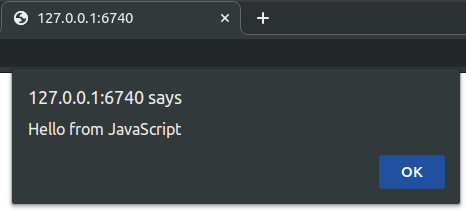
\includegraphics{images/alert.png}
\caption{JavaScript alert in shiny}
\end{figure}

One thing important to note for later is that alerts will always block the execution of code which allows making sure some code is only run with user consent or the user being aware of the consequences.

\begin{Shaded}
\begin{Highlighting}[]
\AttributeTok{alert}\NormalTok{(}\StringTok{\textquotesingle{}delete everything?\textquotesingle{}}\NormalTok{)}\OperatorTok{;}
\AttributeTok{deleteEverythingOnlyIfUserOK}\NormalTok{()}\OperatorTok{;}
\end{Highlighting}
\end{Shaded}

\hypertarget{from-r-to-javascript}{%
\section{From R to JavaScript}\label{from-r-to-javascript}}

Now that we have a simple alert displayed in the application we can tie it with the R server; the alert should display a message sent by the R server, this would enable, for instance, displaying a message taken from a database or a user input. As might be expected there are two functions required to do so, an R function and its JavaScript complementary: one to send the data from the server and another to catch said data from the client and display the alert.

Let us start by writing the R code to send the data, thankfully very little is required of the developer. One can send data from the R server to the client from the \texttt{session} object using the \texttt{sendCustomMessage} method. The method takes two arguments, first an identifier (where to send the data to), second the actual data to send to JavaScript.

\begin{Shaded}
\begin{Highlighting}[]
\NormalTok{server <{-}}\StringTok{ }\ControlFlowTok{function}\NormalTok{(input, output, session)\{}
  \CommentTok{\# set the identifier to send{-}alert}
\NormalTok{  session}\OperatorTok{$}\KeywordTok{sendCustomMessage}\NormalTok{(}
    \DataTypeTok{type =} \StringTok{"send{-}alert"}\NormalTok{, }\DataTypeTok{message =} \StringTok{"Hi there!"}
\NormalTok{  )}
\NormalTok{\}}
\end{Highlighting}
\end{Shaded}

This effectively sends the message to the JavaScript client but we are yet to use that message JavaScript-side so the application still displays the same alert on load. We can add a ``handler'' for the identifier we defined (\texttt{send-alert}) which will so something with the message we sent from the server. This is done with the \texttt{addCustomMessageHandler} method from the \texttt{Shiny} object where the first argument is the identifier and the second is the function that handles the message, a function that takes a single argument: the data sent from the server.

\begin{Shaded}
\begin{Highlighting}[]
\NormalTok{tags}\OperatorTok{$}\KeywordTok{script}\NormalTok{(}
  \StringTok{"Shiny.addCustomMessageHandler(}
\StringTok{    type = \textquotesingle{}send{-}alert\textquotesingle{}, function(message) \{}
\StringTok{      alert(message);}
\StringTok{  \});"}
\NormalTok{)}
\end{Highlighting}
\end{Shaded}

\begin{figure}
\centering
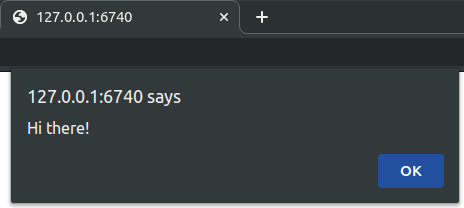
\includegraphics{images/alert-shiny.png}
\caption{Alert sent from shiny server}
\end{figure}

This enables you to pass a message that is taken from a database for instance, or as shown below from a user input, to the alert.

\begin{Shaded}
\begin{Highlighting}[]
\KeywordTok{library}\NormalTok{(shiny)}

\NormalTok{ui <{-}}\StringTok{ }\KeywordTok{fluidPage}\NormalTok{(}
\NormalTok{  tags}\OperatorTok{$}\KeywordTok{script}\NormalTok{(}
    \StringTok{"Shiny.addCustomMessageHandler(}
\StringTok{      type = \textquotesingle{}send{-}alert\textquotesingle{}, function(message) \{}
\StringTok{        alert(message);}
\StringTok{    \});"}
\NormalTok{  ),}
  \KeywordTok{h1}\NormalTok{(}\StringTok{"Hello"}\NormalTok{),}
  \KeywordTok{textInput}\NormalTok{(}\StringTok{"text"}\NormalTok{, }\StringTok{"Text to show in alert"}\NormalTok{),}
  \KeywordTok{actionButton}\NormalTok{(}\StringTok{"submit"}\NormalTok{, }\StringTok{"Show alert"}\NormalTok{)}
\NormalTok{)}

\NormalTok{server <{-}}\StringTok{ }\ControlFlowTok{function}\NormalTok{(input, output, session)\{}
  \KeywordTok{observeEvent}\NormalTok{(input}\OperatorTok{$}\NormalTok{submit, \{}
\NormalTok{    session}\OperatorTok{$}\KeywordTok{sendCustomMessage}\NormalTok{(}\DataTypeTok{type =} \StringTok{"send{-}alert"}\NormalTok{, }\DataTypeTok{message =}\NormalTok{ input}\OperatorTok{$}\NormalTok{text)}
\NormalTok{  \})}
\NormalTok{\}}

\KeywordTok{shinyApp}\NormalTok{(ui, server)}
\end{Highlighting}
\end{Shaded}

In the application above, notice the path that the message follows: it goes from the client to the server which sends it back to the client. This might be considered suboptimal by some as it is not necessary to use the server as intermediary (in this example at least). Though there is some truth to this the above will work perfectly fine---and the aim here is to make JavaScript work with R---not alongside it.

\hypertarget{from-javascript-to-r}{%
\section{From JavaScript to R}\label{from-javascript-to-r}}

Imagine if you will that instead of displaying a somewhat anodyne alert it was one that actually mattered where the user is warned that clicking ``OK'' will execute an irreversible action like the deletion of a record. In order to implement this the server would need to ``know'' whether the user has clicked said ``OK'' button. To do so one needs to pass data from the client to the server.

This can be done by defining a \emph{simplified} shiny input. While one can define a fully-fledged shiny inputs that can be registered, updated, etc. there is also a simplified version of the latter which allows sending reactive input values to the server where it can be used just like any other inputs (\texttt{input\$id}). The value of the input can be defined using the \texttt{setInputValue} method which takes the id of the input and the value to give it.

\begin{Shaded}
\begin{Highlighting}[]
\NormalTok{tags}\OperatorTok{$}\KeywordTok{script}\NormalTok{(}
  \StringTok{"Shiny.addCustomMessageHandler(}
\StringTok{    type = \textquotesingle{}send{-}alert\textquotesingle{}, function(message) \{}
\StringTok{    }
\StringTok{      // show alert}
\StringTok{      alert(message);}

\StringTok{      // set to true when clicked OK}
\StringTok{      Shiny.setInputValue(\textquotesingle{}delete\_alert\textquotesingle{}, true);}
\StringTok{  \});"}
\NormalTok{)}
\end{Highlighting}
\end{Shaded}

As mentioned earlier \texttt{alert} blocks code execution, therefore the input value will not be defined before the button ``OK'' is pressed. The server can now access the \texttt{input\$delete\_alert} input which is by default \texttt{NULL} and set to \texttt{TRUE} when the user has pressed ``OK,'' as done in the application below which prints the input to the console when the button is clicked.

\begin{Shaded}
\begin{Highlighting}[]
\KeywordTok{library}\NormalTok{(shiny)}

\NormalTok{ui <{-}}\StringTok{ }\KeywordTok{fluidPage}\NormalTok{(}
\NormalTok{  tags}\OperatorTok{$}\KeywordTok{script}\NormalTok{(}
    \StringTok{"Shiny.addCustomMessageHandler(}
\StringTok{      type = \textquotesingle{}send{-}alert\textquotesingle{}, function(message) \{}
\StringTok{        alert(message);}
\StringTok{        Shiny.setInputValue(\textquotesingle{}delete\_alert\textquotesingle{}, true);}
\StringTok{    \});"}
\NormalTok{  ),}
  \KeywordTok{h1}\NormalTok{(}\StringTok{"Hello"}\NormalTok{)}
\NormalTok{)}

\NormalTok{server <{-}}\StringTok{ }\ControlFlowTok{function}\NormalTok{(input, output, session)\{}
\NormalTok{  session}\OperatorTok{$}\KeywordTok{sendCustomMessage}\NormalTok{(}
    \DataTypeTok{type =} \StringTok{"send{-}alert"}\NormalTok{, }\DataTypeTok{message =} \StringTok{"Deleting a record!"}
\NormalTok{  )}

  \KeywordTok{observeEvent}\NormalTok{(input}\OperatorTok{$}\NormalTok{delete\_alert, \{}
    \CommentTok{\# print TRUE when button is clicked}
    \KeywordTok{print}\NormalTok{(input}\OperatorTok{$}\NormalTok{delete\_alert) }
\NormalTok{  \})}
\NormalTok{\}}

\KeywordTok{shinyApp}\NormalTok{(ui, server)}
\end{Highlighting}
\end{Shaded}

Note that Shiny performs optimisations on how those values are set. First, if the input is set to the same value then Shiny ignores it. This is fine if you are interested in the actual value of the input but will not work as expected if the input is to be used as event. Indeed if you want to use this input in an \texttt{observe}, \texttt{observeEvent}, or \texttt{eventReactive}, you want it to be triggered every time the input changes, regardless of whether that value is the same as before. The second optimisation Shiny does is when the input is set to multiple different values before these have been processed then only the most recent value will actually be sent to the server. One can opt-out of these optimisations using the \texttt{priority:\ "event"} option when setting the input value.

\begin{Shaded}
\begin{Highlighting}[]
\KeywordTok{library}\NormalTok{(shiny)}

\NormalTok{ui <{-}}\StringTok{ }\KeywordTok{fluidPage}\NormalTok{(}
\NormalTok{  tags}\OperatorTok{$}\KeywordTok{script}\NormalTok{(}
    \StringTok{"Shiny.addCustomMessageHandler(}
\StringTok{      type = \textquotesingle{}send{-}alert\textquotesingle{}, function(message) \{}
\StringTok{        alert(message);}
\StringTok{        Shiny.setInputValue(\textquotesingle{}delete\_alert\textquotesingle{}, true, \{priority: \textquotesingle{}event\textquotesingle{}\});}
\StringTok{    \});"}
\NormalTok{  ),}
  \KeywordTok{h1}\NormalTok{(}\StringTok{"Hello"}\NormalTok{)}
\NormalTok{)}

\NormalTok{server <{-}}\StringTok{ }\ControlFlowTok{function}\NormalTok{(input, output, session)\{}
\NormalTok{  session}\OperatorTok{$}\KeywordTok{sendCustomMessage}\NormalTok{(}
    \DataTypeTok{type =} \StringTok{"send{-}alert"}\NormalTok{, }\DataTypeTok{message =} \StringTok{"Deleting a record!"}
\NormalTok{  )}

  \KeywordTok{observeEvent}\NormalTok{(input}\OperatorTok{$}\NormalTok{delete\_alert, \{}
    \CommentTok{\# print TRUE when button is clicked}
    \KeywordTok{print}\NormalTok{(input}\OperatorTok{$}\NormalTok{delete\_alert) }
\NormalTok{  \})}
\NormalTok{\}}

\KeywordTok{shinyApp}\NormalTok{(ui, server)}
\end{Highlighting}
\end{Shaded}

\begin{verbatim}
## [1] TRUE
\end{verbatim}

\hypertarget{deserialise}{%
\section{Deserialise}\label{deserialise}}

In the section on sending data from R to JavaScript we used a ``message handler'' in JavaScript to handle the data coming from the server. There is also the corollary, an ``input handler'' to preprocess the data coming from JavaScript before it is made accessible by the input. In R, this is a function that must accept three arguments, the data coming JavaScript, a shiny session, and the name of the input. Note that all of these arguments are mandatory even if they are used in the function.

Input handlers are most often used to reshape or change the type of the data coming in. To demonstrate how use them, we create a handler for the \texttt{delete\_alert} which adds somewhat useless meta information to the data.

\begin{Shaded}
\begin{Highlighting}[]
\CommentTok{\# create handler}
\NormalTok{process\_input <{-}}\StringTok{ }\ControlFlowTok{function}\NormalTok{(x, session, inputname)\{}
\NormalTok{  data <{-}}\StringTok{ }\KeywordTok{list}\NormalTok{(}
    \DataTypeTok{data =}\NormalTok{ x,}
    \DataTypeTok{meta =} \StringTok{"This is some meta{-}data"}
\NormalTok{  )}
  \KeywordTok{return}\NormalTok{(data)}
\NormalTok{\}}
\end{Highlighting}
\end{Shaded}

Once this function created it needs to be registered with shiny using the \texttt{registerInputHandler} function which takes two arguments. First, a unique identifier for the handler, second, the handler function. Attempt to give the handler a unique yet simple name (alphanumeric characters, underscores, and periods) to avoid clashes with other handlers.

\begin{Shaded}
\begin{Highlighting}[]
\CommentTok{\# register with shiny}
\KeywordTok{registerInputHandler}\NormalTok{(}\StringTok{"alert.processor"}\NormalTok{, process\_input)}
\end{Highlighting}
\end{Shaded}

Note that handlers can only be registered once, running the above twice will fail the second time, even if the handler function has changed. Thus, the handler can be overwritten by setting \texttt{force} to \texttt{TRUE}.

\begin{Shaded}
\begin{Highlighting}[]
\CommentTok{\# register with shiny}
\KeywordTok{registerInputHandler}\NormalTok{(}\StringTok{"alert.processor"}\NormalTok{, process\_input, }\DataTypeTok{force =} \OtherTok{TRUE}\NormalTok{)}
\end{Highlighting}
\end{Shaded}

Once the handler function created and registered with shiny what is left to do is tell shiny which input should use that handler. This is done by adding the name of the handler, \texttt{alert.processor}, preceded by a colon (\texttt{:alert.processor}) as a suffix to the input name.

\begin{Shaded}
\begin{Highlighting}[]
\VariableTok{Shiny}\NormalTok{.}\AttributeTok{setInputValue}\NormalTok{(}\StringTok{\textquotesingle{}delete\_alert:alert.processor\textquotesingle{}}\OperatorTok{,} \KeywordTok{true}\OperatorTok{,} \OperatorTok{\{}\DataTypeTok{priority}\OperatorTok{:} \StringTok{\textquotesingle{}event\textquotesingle{}}\OperatorTok{\}}\NormalTok{)}\OperatorTok{;}
\end{Highlighting}
\end{Shaded}

We can then recap to see what the application would look like now.

\begin{Shaded}
\begin{Highlighting}[]
\KeywordTok{library}\NormalTok{(shiny)}

\CommentTok{\# create handler}
\NormalTok{process\_input <{-}}\StringTok{ }\ControlFlowTok{function}\NormalTok{(x, session, inputname)\{}
\NormalTok{  data <{-}}\StringTok{ }\KeywordTok{list}\NormalTok{(}
    \DataTypeTok{data =}\NormalTok{ x,}
    \DataTypeTok{meta =} \StringTok{"This is some meta{-}data"}
\NormalTok{  )}
  \KeywordTok{return}\NormalTok{(data)}
\NormalTok{\}}

\CommentTok{\# register with shiny}
\KeywordTok{registerInputHandler}\NormalTok{(}\StringTok{"alert.processor"}\NormalTok{, process\_input)}

\NormalTok{ui <{-}}\StringTok{ }\KeywordTok{fluidPage}\NormalTok{(}
\NormalTok{  tags}\OperatorTok{$}\KeywordTok{script}\NormalTok{(}
    \StringTok{"Shiny.addCustomMessageHandler(}
\StringTok{      type = \textquotesingle{}send{-}alert\textquotesingle{}, function(message) \{}
\StringTok{        alert(message);}
\StringTok{        Shiny.setInputValue(}
\StringTok{          \textquotesingle{}delete\_alert:alert.processor\textquotesingle{}, true, }
\StringTok{          \{priority: \textquotesingle{}event\textquotesingle{}\}}
\StringTok{        );}
\StringTok{    \});"}
\NormalTok{  ),}
  \KeywordTok{h1}\NormalTok{(}\StringTok{"Hello"}\NormalTok{)}
\NormalTok{)}

\NormalTok{server <{-}}\StringTok{ }\ControlFlowTok{function}\NormalTok{(input, output, session)\{}
\NormalTok{  session}\OperatorTok{$}\KeywordTok{sendCustomMessage}\NormalTok{(}
    \DataTypeTok{type =} \StringTok{"send{-}alert"}\NormalTok{, }\DataTypeTok{message =} \StringTok{"Deleting a record!"}
\NormalTok{  )}

  \KeywordTok{observeEvent}\NormalTok{(input}\OperatorTok{$}\NormalTok{delete\_alert, \{}
    \KeywordTok{print}\NormalTok{(input}\OperatorTok{$}\NormalTok{delete\_alert) }
\NormalTok{  \})}
\NormalTok{\}}

\KeywordTok{shinyApp}\NormalTok{(ui, server)}
\end{Highlighting}
\end{Shaded}

\begin{verbatim}
## $data
## [1] TRUE
## 
## $meta
## [1] "This is some meta-data"
\end{verbatim}

The previous section on the input handler is entirely optional but as we will see in later parts of the book it can be nice touch in some cases.

\hypertarget{a-complete-integration}{%
\chapter{A Complete Integration}\label{a-complete-integration}}

Thus far, this part of the book has covered both ways data travels between JavaScript and R in Shiny. However, the alerts displayed in the previous chapter are rather hideous and, though demonstrates how both languages can work together within shiny, comes short of illustrating how to make use of external libraries or how to package such code. In brief, the previous chapter is an interesting exercise but unlikely to be used in the real world. This chapter is different.

Let's exploit an external library to improve upon the work done so far: \href{https://github.com/StephanWagner/jBox}{jBox} allows displaying ``notices,'' similar to the vanilla JavaScript alerts, but much better looking and with additional functionalities.

The very first thing to do is to import jBox in the project, we could download the files and use them as described in the previous static files section but it comes with very convenient CDNs detailed in the \href{https://stephanwagner.me/jBox/get_started}{get-started page} of the documentation.

\begin{Shaded}
\begin{Highlighting}[]
\KeywordTok{<script}\OtherTok{ src=}\StringTok{"https://code.jquery.com/jquery{-}3.5.1.min.js"}\KeywordTok{></script>}
\KeywordTok{<script}\OtherTok{ src=}\StringTok{"https://cdn.jsdelivr.net/gh/StephanWagner/jBox@v1.2.0/dist/jBox.all.min.js"}\KeywordTok{></script>}
\KeywordTok{<link}\OtherTok{ href=}\StringTok{"https://cdn.jsdelivr.net/gh/StephanWagner/jBox@v1.2.0/dist/jBox.all.min.css"}\OtherTok{ rel=}\StringTok{"stylesheet"}\KeywordTok{>}
\end{Highlighting}
\end{Shaded}

Note that the ``j'' in jBox stands for jQuery which is already a dependency of shiny itself, there is therefore no need to import it, on the contrary one should not in order to avoid clashes. We can import the dependencies in a shiny UI, along with a message handler.

\begin{Shaded}
\begin{Highlighting}[]
\NormalTok{ui <{-}}\StringTok{ }\KeywordTok{fluidPage}\NormalTok{(}
\NormalTok{  tags}\OperatorTok{$}\KeywordTok{head}\NormalTok{(}
\NormalTok{    tags}\OperatorTok{$}\KeywordTok{script}\NormalTok{(}
      \DataTypeTok{src =} \KeywordTok{paste0}\NormalTok{(}
        \StringTok{"https://cdn.jsdelivr.net/gh/StephanWagner/"}\NormalTok{,}
        \StringTok{"jBox@v1.2.0/dist/jBox.all.min.js"}
\NormalTok{      )}
\NormalTok{    ),}
\NormalTok{    tags}\OperatorTok{$}\KeywordTok{link}\NormalTok{(}
      \DataTypeTok{rel =} \StringTok{"stylesheet"}\NormalTok{,}
      \DataTypeTok{href =} \KeywordTok{paste0}\NormalTok{(}
        \StringTok{"https://cdn.jsdelivr.net/gh/StephanWagner/"}\NormalTok{,}
        \StringTok{"jBox@v1.2.0/dist/jBox.all.min.css"}
\NormalTok{      )}
\NormalTok{    ),}
\NormalTok{    tags}\OperatorTok{$}\KeywordTok{script}\NormalTok{(}\StringTok{"Shiny.addCustomMessageHandler(}
\StringTok{      type = \textquotesingle{}send{-}alert\textquotesingle{}, function(message) \{}
\StringTok{      // TO DO: code jBox}
\StringTok{    \});"}\NormalTok{)}
\NormalTok{  )}
\NormalTok{)}
\end{Highlighting}
\end{Shaded}

The jBox library comes with numerous features to display tooltips, modals, notices, and more, which would make for too long a chapter; only notices shall be covered here. Let's first take a look at the code that generates a jBox notice.

\begin{Shaded}
\begin{Highlighting}[]
\KeywordTok{new} \AttributeTok{jBox}\NormalTok{(}\StringTok{\textquotesingle{}Notice\textquotesingle{}}\OperatorTok{,} \OperatorTok{\{}
  \DataTypeTok{content}\OperatorTok{:} \StringTok{\textquotesingle{}Hurray! A notice!\textquotesingle{}}\OperatorTok{,}
  \DataTypeTok{color}\OperatorTok{:} \StringTok{\textquotesingle{}blue\textquotesingle{}}
\OperatorTok{\}}\NormalTok{)}\OperatorTok{;}
\end{Highlighting}
\end{Shaded}

Let's start by copying that in the message handler to observe what it looks like.

\begin{Shaded}
\begin{Highlighting}[]
\KeywordTok{library}\NormalTok{(shiny)}

\NormalTok{ui <{-}}\StringTok{ }\KeywordTok{fluidPage}\NormalTok{(}
\NormalTok{  tags}\OperatorTok{$}\KeywordTok{head}\NormalTok{(}
\NormalTok{    tags}\OperatorTok{$}\KeywordTok{script}\NormalTok{(}
      \DataTypeTok{src =} \KeywordTok{paste0}\NormalTok{(}
        \StringTok{"https://cdn.jsdelivr.net/gh/StephanWagner/"}\NormalTok{,}
        \StringTok{"jBox@v1.2.0/dist/jBox.all.min.js"}
\NormalTok{      )}
\NormalTok{    ),}
\NormalTok{    tags}\OperatorTok{$}\KeywordTok{link}\NormalTok{(}
      \DataTypeTok{rel =} \StringTok{"stylesheet"}\NormalTok{,}
      \DataTypeTok{href =} \KeywordTok{paste0}\NormalTok{(}
        \StringTok{"https://cdn.jsdelivr.net/gh/StephanWagner/"}\NormalTok{,}
        \StringTok{"jBox@v1.2.0/dist/jBox.all.min.css"}
\NormalTok{      )}
\NormalTok{    ),}
\NormalTok{    tags}\OperatorTok{$}\KeywordTok{script}\NormalTok{(}\StringTok{"Shiny.addCustomMessageHandler(}
\StringTok{      type = \textquotesingle{}send{-}alert\textquotesingle{}, function(message) \{}
\StringTok{        new jBox(\textquotesingle{}Notice\textquotesingle{}, \{}
\StringTok{          content: \textquotesingle{}Hurray! A notice!\textquotesingle{},}
\StringTok{          color: \textquotesingle{}blue\textquotesingle{}}
\StringTok{        \});}
\StringTok{    \});"}\NormalTok{)}
\NormalTok{  )}
\NormalTok{)}

\NormalTok{server <{-}}\StringTok{ }\ControlFlowTok{function}\NormalTok{(input, output, session)\{}
\NormalTok{  session}\OperatorTok{$}\KeywordTok{sendCustomMessage}\NormalTok{(}
    \DataTypeTok{type =} \StringTok{"send{-}alert"}\NormalTok{, }\DataTypeTok{message =} \StringTok{"This is not used"}
\NormalTok{  )}
\NormalTok{\}}

\KeywordTok{shinyApp}\NormalTok{(ui, server)}
\end{Highlighting}
\end{Shaded}

\begin{figure}
\centering

\includegraphics{images/notice-1.png}
\caption{First jBox Notice}
\end{figure}

With some minor changes the application can display the message passed, one only needs to replace `Hurray! A notice!' with the \texttt{message} variable.

\begin{Shaded}
\begin{Highlighting}[]
\NormalTok{tags}\OperatorTok{$}\KeywordTok{script}\NormalTok{(}\StringTok{"Shiny.addCustomMessageHandler(}
\StringTok{  type = \textquotesingle{}send{-}alert\textquotesingle{}, function(message) \{}
\StringTok{    new jBox(\textquotesingle{}Notice\textquotesingle{}, \{}
\StringTok{      content: message,}
\StringTok{      color: \textquotesingle{}blue\textquotesingle{}}
\StringTok{    \});}
\StringTok{\});"}\NormalTok{)}
\end{Highlighting}
\end{Shaded}

This though only allows passing a single variable, the message, to JavaScript but jBox has many more options.

\hypertarget{serialisation}{%
\section{Serialisation}\label{serialisation}}

Let's delve deeper into the communication between the server and the front-end to understand how we can further customise the notice displayed, e.g.: change the colour.

\begin{Shaded}
\begin{Highlighting}[]
\OperatorTok{\{}
  \DataTypeTok{content}\OperatorTok{:} \StringTok{\textquotesingle{}Hurray! A notice!\textquotesingle{}}\OperatorTok{,}
  \DataTypeTok{color}\OperatorTok{:} \StringTok{\textquotesingle{}blue\textquotesingle{}}
\OperatorTok{\}}
\end{Highlighting}
\end{Shaded}

Notice that the jBox notice takes a JSON object containing the options that define said notice to display (example above), including but not limited to the message. The most straightforward way to make all those options accessible to the server is to construct that list of options server-side before sending it to the the front-end. For instance the JSON of options displayed above would look like the R list below.

\begin{Shaded}
\begin{Highlighting}[]
\NormalTok{options <{-}}\StringTok{ }\KeywordTok{list}\NormalTok{(}
  \DataTypeTok{content =} \StringTok{\textquotesingle{}Hurray! A notice!\textquotesingle{}}\NormalTok{,}
  \DataTypeTok{color =} \StringTok{\textquotesingle{}blue\textquotesingle{}}
\NormalTok{)}

\NormalTok{jsonlite}\OperatorTok{::}\KeywordTok{toJSON}\NormalTok{(options, }\DataTypeTok{pretty =} \OtherTok{TRUE}\NormalTok{, }\DataTypeTok{auto\_unbox =} \OtherTok{TRUE}\NormalTok{)}
\end{Highlighting}
\end{Shaded}

\begin{verbatim}
## {
##   "content": "Hurray! A notice!",
##   "color": "blue"
## }
\end{verbatim}

Therefore one could construct this list server-side and use it in jBox straight away, doing so means the JavaScript code can be simplified to \texttt{new\ jBox(\textquotesingle{}Notice\textquotesingle{},\ message);}.

\begin{Shaded}
\begin{Highlighting}[]
\KeywordTok{library}\NormalTok{(shiny)}

\NormalTok{ui <{-}}\StringTok{ }\KeywordTok{fluidPage}\NormalTok{(}
\NormalTok{  tags}\OperatorTok{$}\KeywordTok{head}\NormalTok{(}
\NormalTok{    tags}\OperatorTok{$}\KeywordTok{script}\NormalTok{(}
      \DataTypeTok{src =} \KeywordTok{paste0}\NormalTok{(}
        \StringTok{"https://cdn.jsdelivr.net/gh/StephanWagner/"}\NormalTok{,}
        \StringTok{"jBox@v1.2.0/dist/jBox.all.min.js"}
\NormalTok{      )}
\NormalTok{    ),}
\NormalTok{    tags}\OperatorTok{$}\KeywordTok{link}\NormalTok{(}
      \DataTypeTok{rel =} \StringTok{"stylesheet"}\NormalTok{,}
      \DataTypeTok{href =} \KeywordTok{paste0}\NormalTok{(}
        \StringTok{"https://cdn.jsdelivr.net/gh/StephanWagner/"}\NormalTok{,}
        \StringTok{"jBox@v1.2.0/dist/jBox.all.min.css"}
\NormalTok{      )}
\NormalTok{    ),}
\NormalTok{    tags}\OperatorTok{$}\KeywordTok{script}\NormalTok{(}\StringTok{"Shiny.addCustomMessageHandler(}
\StringTok{      type = \textquotesingle{}send{-}alert\textquotesingle{}, function(message) \{}
\StringTok{        // use notice send from the server}
\StringTok{        new jBox(\textquotesingle{}Notice\textquotesingle{}, message);}
\StringTok{    \});"}\NormalTok{)}
\NormalTok{  )}
\NormalTok{)}

\NormalTok{server <{-}}\StringTok{ }\ControlFlowTok{function}\NormalTok{(input, output, session)\{}

  \CommentTok{\# define notice options}
\NormalTok{  notice =}\StringTok{ }\KeywordTok{list}\NormalTok{(}
    \DataTypeTok{content =} \StringTok{\textquotesingle{}Hello from the server\textquotesingle{}}\NormalTok{,}
    \DataTypeTok{color =} \StringTok{\textquotesingle{}black\textquotesingle{}}
\NormalTok{  )}

  \CommentTok{\# send the notice}
\NormalTok{  session}\OperatorTok{$}\KeywordTok{sendCustomMessage}\NormalTok{(}\DataTypeTok{type =} \StringTok{"send{-}alert"}\NormalTok{, }\DataTypeTok{message =}\NormalTok{ notice)}
\NormalTok{\}}

\KeywordTok{shinyApp}\NormalTok{(ui, server)}
\end{Highlighting}
\end{Shaded}

\begin{figure}
\centering

\includegraphics{images/notice-2.png}
\caption{Customised jBox Notice}
\end{figure}

\hypertarget{events-callbacks}{%
\section{Events \& Callbacks}\label{events-callbacks}}

In the example of the vanilla JavaScript alert one could simply place a line of code after the \texttt{alert()} function in order to ``tell'' the server whether the button on the alert had been clicked. This was feasible because \texttt{alert} stops code execution, this is, however, rather uncommon in JavaScript. What is far more common are events and callback functions which are triggered upon an action being performed by the user (like the click of a button) or when other interesting things happen in the code. jBox provides numerous such \href{https://stephanwagner.me/jBox/options\#events}{events}; callback functions can be used when a modal is closed or when a notice is created for instance.

The concept of the callback function is not totally foreign to R albeit rarely used. Shiny comes with such functions, \texttt{shiny::onStop} and \texttt{shiny::onStart}. These allows having functions run when the application starts or exits.

\begin{Shaded}
\begin{Highlighting}[]
\NormalTok{server <{-}}\StringTok{ }\ControlFlowTok{function}\NormalTok{(input, output)\{}
\NormalTok{  shiny}\OperatorTok{::}\KeywordTok{onStop}\NormalTok{(}
    \CommentTok{\# callback function fired when app is closed}
    \ControlFlowTok{function}\NormalTok{()\{}
      \KeywordTok{cat}\NormalTok{(}\StringTok{"App has been closed"}\NormalTok{)}
\NormalTok{    \}}
\NormalTok{  )}
\NormalTok{\}}
\end{Highlighting}
\end{Shaded}

In jBox, these callback functions are included in the JSON of options, below the \texttt{onClose} event is fired when the notice is closed.

\begin{Shaded}
\begin{Highlighting}[]
\OperatorTok{\{}
  \DataTypeTok{content}\OperatorTok{:} \StringTok{\textquotesingle{}Alert!\textquotesingle{}}\OperatorTok{,}
  \DataTypeTok{onClose}\OperatorTok{:} \KeywordTok{function}\NormalTok{()}\OperatorTok{\{}
    \CommentTok{// Fired when closed }
    \VariableTok{console}\NormalTok{.}\AttributeTok{log}\NormalTok{(}\StringTok{\textquotesingle{}Alert is closed\textquotesingle{}}\NormalTok{)}\OperatorTok{;}
  \OperatorTok{\}}
\OperatorTok{\}}
\end{Highlighting}
\end{Shaded}

This raises one issue, one cannot truly serialise to executable code. The attempt below serialises the function to a string, not a function that will be evaluated in JavaScript.

\begin{Shaded}
\begin{Highlighting}[]
\CommentTok{\# try to serialise an R function}
\NormalTok{jsonlite}\OperatorTok{::}\KeywordTok{toJSON}\NormalTok{(}\StringTok{"function(x)\{x + 1\}"}\NormalTok{)}
\end{Highlighting}
\end{Shaded}

\begin{verbatim}
## ["function(x){x + 1}"]
\end{verbatim}

One solution is to append the callback function to the object of options JavaScript-side.

\begin{Shaded}
\begin{Highlighting}[]
\NormalTok{tags}\OperatorTok{$}\KeywordTok{script}\NormalTok{(}\StringTok{"Shiny.addCustomMessageHandler(}
\StringTok{  type = \textquotesingle{}send{-}alert\textquotesingle{}, function(message) \{}
\StringTok{    // append callback}
\StringTok{    message.onClose = function()\{}
\StringTok{      Shiny.setInputValue(\textquotesingle{}alert\_close\textquotesingle{}, true);}
\StringTok{    \}}
\StringTok{    new jBox(\textquotesingle{}Notice\textquotesingle{}, message);}
\StringTok{\});"}\NormalTok{)}
\end{Highlighting}
\end{Shaded}

Placing a function inside a JSON object is common in JavaScript, in contrast with R where though it works is rarely if ever done (reference class/R6 are somewhat similar). The above JavaScript code to append the callback function could look something like the snippet below in R.

\begin{Shaded}
\begin{Highlighting}[]
\NormalTok{message <{-}}\StringTok{ }\KeywordTok{list}\NormalTok{(}\DataTypeTok{content =} \StringTok{"hello"}\NormalTok{)}
\NormalTok{message}\OperatorTok{$}\NormalTok{onClose <{-}}\StringTok{ }\ControlFlowTok{function}\NormalTok{(x)\{}
\NormalTok{  x }\OperatorTok{+}\StringTok{ }\DecValTok{1}
\NormalTok{\}}

\NormalTok{message}\OperatorTok{$}\KeywordTok{onClose}\NormalTok{(}\DecValTok{2}\NormalTok{)}
\end{Highlighting}
\end{Shaded}

\begin{verbatim}
## [1] 3
\end{verbatim}

That done it can be incorporated into the application built thus far. Something interesting could be done server-side but for the sake of this example we merely print the value of the input to the R console.

\begin{Shaded}
\begin{Highlighting}[]
\KeywordTok{library}\NormalTok{(shiny)}

\NormalTok{ui <{-}}\StringTok{ }\KeywordTok{fluidPage}\NormalTok{(}
\NormalTok{  tags}\OperatorTok{$}\KeywordTok{head}\NormalTok{(}
\NormalTok{    tags}\OperatorTok{$}\KeywordTok{script}\NormalTok{(}
      \DataTypeTok{src =} \KeywordTok{paste0}\NormalTok{(}
        \StringTok{"https://cdn.jsdelivr.net/gh/StephanWagner/"}\NormalTok{,}
        \StringTok{"jBox@v1.2.0/dist/jBox.all.min.js"}
\NormalTok{      )}
\NormalTok{    ),}
\NormalTok{    tags}\OperatorTok{$}\KeywordTok{link}\NormalTok{(}
      \DataTypeTok{rel =} \StringTok{"stylesheet"}\NormalTok{,}
      \DataTypeTok{href =} \KeywordTok{paste0}\NormalTok{(}
        \StringTok{"https://cdn.jsdelivr.net/gh/StephanWagner/"}\NormalTok{,}
        \StringTok{"jBox@v1.2.0/dist/jBox.all.min.css"}
\NormalTok{      )}
\NormalTok{    ),}
\NormalTok{    tags}\OperatorTok{$}\KeywordTok{script}\NormalTok{(}\StringTok{"Shiny.addCustomMessageHandler(}
\StringTok{      type = \textquotesingle{}send{-}alert\textquotesingle{}, function(message) \{}
\StringTok{        message.onClose = function()\{}
\StringTok{          Shiny.setInputValue(\textquotesingle{}alert\_close\textquotesingle{}, true);}
\StringTok{        \}}
\StringTok{        new jBox(\textquotesingle{}Notice\textquotesingle{}, message);}
\StringTok{    \});"}\NormalTok{)}
\NormalTok{  )}
\NormalTok{)}

\NormalTok{server <{-}}\StringTok{ }\ControlFlowTok{function}\NormalTok{(input, output, session)\{}

  \CommentTok{\# define notice options}
\NormalTok{  notice =}\StringTok{ }\KeywordTok{list}\NormalTok{(}
    \DataTypeTok{content =} \StringTok{\textquotesingle{}Hello from the server\textquotesingle{}}\NormalTok{,}
    \DataTypeTok{color =} \StringTok{\textquotesingle{}black\textquotesingle{}}
\NormalTok{  )}

  \CommentTok{\# send the notice}
\NormalTok{  session}\OperatorTok{$}\KeywordTok{sendCustomMessage}\NormalTok{(}
    \DataTypeTok{type =} \StringTok{"send{-}alert"}\NormalTok{, }\DataTypeTok{message =}\NormalTok{ notice}
\NormalTok{  )}

  \CommentTok{\# print the output of the alert\_close event (when fired)}
  \KeywordTok{observeEvent}\NormalTok{(input}\OperatorTok{$}\NormalTok{alert\_close, \{}
    \KeywordTok{print}\NormalTok{(input}\OperatorTok{$}\NormalTok{alert\_close)}
\NormalTok{  \})}
\NormalTok{\}}

\KeywordTok{shinyApp}\NormalTok{(ui, server)}
\end{Highlighting}
\end{Shaded}

\hypertarget{as-a-package}{%
\section{As a Package}\label{as-a-package}}

Packages are a fundamental part of R and allow conveniently sharing and reusing code. The work done so far is probably fitting for a single application but one should not have to reproduce all of that every time one wants to use jBox in a shiny application: we ought to wrap these functionalities into a handy package that can be used, reused and shared with others. Moreover, this will benefit from all the other advantages that R packages bring to code such as documentation, reproducibility, and tests.

Before we delve into building the package let us think through what it should include. The application using jBox gives some indication as to what the package will look like. Users of the package should be able to reproduce what is executed in the application, namely import dependencies (including the message handler) as well as send data to the JavaScript front-end. One difference with the application is the provision of a static directory of dependencies to avoid relying on the CDNs as this ensures reproducibility and more robustness (code hosted online by a third-party might change and break the package). Concretely, the package will export a \texttt{useJbox} function to be placed in the shiny ui to import the dependencies and a \texttt{send\_alert} function to send the alert from the server to the client.

Let's start by creating an R package, here we name it ``jbox,'' after the JavaScript library, partly because the author lacks creativity: feel free to name it however you want.

\begin{Shaded}
\begin{Highlighting}[]
\NormalTok{usethis}\OperatorTok{::}\KeywordTok{create\_package}\NormalTok{(}\StringTok{"jbox"}\NormalTok{)}
\end{Highlighting}
\end{Shaded}

\hypertarget{dependencies}{%
\subsection{Dependencies}\label{dependencies}}

The very first thing that is required are the dependencies without which nothing can work, let's create a directory of static assets, download and place the jBox CSS and JavaScript files within it. We create the directory ``inst'' as per the R package convention and within it create another to hold the assets.

\begin{Shaded}
\begin{Highlighting}[]
\CommentTok{\# create directories}
\KeywordTok{dir.create}\NormalTok{(}\StringTok{"inst/assets"}\NormalTok{, }\DataTypeTok{recursive =} \OtherTok{TRUE}\NormalTok{)}
\end{Highlighting}
\end{Shaded}

The jBox files can be downloaded from the CDN and placed within the directory that was created above. Moreover, we also create an empty JavaScript file that will eventually contain the custom JavaScript code that ``connects'' R to JavaScript.

\begin{Shaded}
\begin{Highlighting}[]
\CommentTok{\# URLs of CDNs}
\NormalTok{js\_dep <{-}}\StringTok{ }\KeywordTok{paste0}\NormalTok{(}
  \StringTok{"https://cdn.jsdelivr.net/gh/StephanWagner/"}\NormalTok{,}
  \StringTok{"jBox@v1.2.0/dist/jBox.all.min.js"}
\NormalTok{)}
\NormalTok{css\_dep <{-}}\StringTok{ }\KeywordTok{paste0}\NormalTok{(}
  \StringTok{"https://cdn.jsdelivr.net/gh/StephanWagner/"}\NormalTok{,}
  \StringTok{"jBox@v1.2.0/dist/jBox.all.min.css"}
\NormalTok{)}

\CommentTok{\# download}
\KeywordTok{download.file}\NormalTok{(js\_dep, }\DataTypeTok{destfile=}\StringTok{"./inst/assets/jBox.all.min.js"}\NormalTok{)}
\KeywordTok{download.file}\NormalTok{(css\_dep, }\DataTypeTok{destfile=}\StringTok{"./inst/assets/jBox.all.min.css"}\NormalTok{)}

\CommentTok{\# create file to eventually hold custom JavaScript}
\KeywordTok{file.create}\NormalTok{(}\StringTok{"./inst/assets/custom.js"}\NormalTok{)}
\end{Highlighting}
\end{Shaded}

This done one should obtain a directory that looks similar to the tree below (some files and folders omitted for brevity).

\begin{Shaded}
\begin{Highlighting}[]
\ExtensionTok{DESCRIPTION}
\ExtensionTok{R/}
\ExtensionTok{inst/}
\NormalTok{├── }\ExtensionTok{assets/}
\NormalTok{│    ├── }\ExtensionTok{custom.js}
\NormalTok{│    ├── }\ExtensionTok{jBox.all.min.js}
\NormalTok{│    └── }\ExtensionTok{jBox.all.min.css}
\end{Highlighting}
\end{Shaded}

Next, one needs to have those files served, the user of the package could be asked to use \texttt{shiny::addResourcePath} but it's very inelegant, it should instead be built-in the package so the user does not even have to know this happening in the background. Therefore, we ought to ensure the static files are served when the user uses the package. Packages can optionally run functions when they are loaded or attached, Hadley Wickham writes about it extensively in the namespace chapter of his book on \href{http://r-pkgs.had.co.nz/namespace.html}{R packages}. By convention, these functions are placed in a \texttt{zzz.R} file.

\begin{Shaded}
\begin{Highlighting}[]
\KeywordTok{file.create}\NormalTok{(}\StringTok{"./R/zzz.R"}\NormalTok{)}
\end{Highlighting}
\end{Shaded}

The difference between loading and attaching a package can be subtle, in this case it's probably best to run the function when the package is loaded using \texttt{.onLoad} which the R Packages book describes as:

\begin{quote}
Loading will load code, data and any DLLs; register S3 and S4 methods; and run the .onLoad() function. After loading, the package is available in memory, but because it's not in the search path, you won't be able to access its components without using ::. Confusingly, :: will also load a package automatically if it isn't already loaded. It's rare to load a package explicitly, but you can do so with requireNamespace() or loadNamespace().

\VA{--- R Packages Book}{}
\end{quote}

The \texttt{addResourcePath} function should thus be placed within the \texttt{.onLoad} function, this way the files are served by shiny when the package is loaded. Note the few changes below, we refer to the path using \texttt{system.file} and change the prefix to \texttt{jbox-assets} to avoid the url serving the static files to clash with others.

\begin{Shaded}
\begin{Highlighting}[]
\CommentTok{\# R/zzz.R}
\NormalTok{.onLoad <{-}}\StringTok{ }\ControlFlowTok{function}\NormalTok{(libname, pkgname) \{}
\NormalTok{  path <{-}}\StringTok{ }\KeywordTok{system.file}\NormalTok{(}\StringTok{"assets"}\NormalTok{, }\DataTypeTok{package =} \StringTok{"jbox"}\NormalTok{)}
\NormalTok{  shiny}\OperatorTok{::}\KeywordTok{addResourcePath}\NormalTok{(}\StringTok{"jbox{-}assets"}\NormalTok{, path)}
\NormalTok{\}}
\end{Highlighting}
\end{Shaded}

This serves the file and allows not having to explicitly use \texttt{addResourcePath} but the package nonetheless needs to feature a function to let the user import them into their application.

\begin{Shaded}
\begin{Highlighting}[]
\CommentTok{\#\textquotesingle{} Import Dependencies}
\CommentTok{\#\textquotesingle{} @export}
\NormalTok{usejBox <{-}}\StringTok{ }\ControlFlowTok{function}\NormalTok{()\{}
\NormalTok{  shiny}\OperatorTok{::}\NormalTok{tags}\OperatorTok{$}\KeywordTok{head}\NormalTok{(}
\NormalTok{    shiny}\OperatorTok{::}\NormalTok{tags}\OperatorTok{$}\KeywordTok{script}\NormalTok{(}
      \DataTypeTok{src =} \StringTok{"jbox{-}assets/jBox.all.min.js"}
\NormalTok{    ),}
\NormalTok{    shiny}\OperatorTok{::}\NormalTok{tags}\OperatorTok{$}\KeywordTok{link}\NormalTok{(}
      \DataTypeTok{rel =} \StringTok{"stylesheet"}\NormalTok{, }
      \DataTypeTok{href =} \StringTok{"jbox{-}assets/jBox.all.min.css"}
\NormalTok{    ),}
\NormalTok{    shiny}\OperatorTok{::}\NormalTok{tags}\OperatorTok{$}\KeywordTok{script}\NormalTok{(}
      \DataTypeTok{src =} \StringTok{"jbox{-}assets/custom.js"}
\NormalTok{    )}
\NormalTok{  )}
\NormalTok{\}}
\end{Highlighting}
\end{Shaded}

\hypertarget{r-code}{%
\subsection{R Code}\label{r-code}}

Not much changes from what was written before, however, it poses interesting questions with regard to the interface we want to provide users. From the user's perspective the core of the package is the function that actually sends an alert to the clients, here created in \texttt{R/core.R}.

\begin{Shaded}
\begin{Highlighting}[]
\CommentTok{\#\textquotesingle{} Create an Alert}
\CommentTok{\#\textquotesingle{} @export}
\NormalTok{send\_alert <{-}}\StringTok{ }\ControlFlowTok{function}\NormalTok{(}\DataTypeTok{content =} \StringTok{"alert"}\NormalTok{, }\DataTypeTok{color =} \StringTok{"blue"}\NormalTok{, session)\{}
  \CommentTok{\# define notice options}
\NormalTok{  notice =}\StringTok{ }\KeywordTok{list}\NormalTok{(}\DataTypeTok{content =}\NormalTok{ content, }\DataTypeTok{color =} \StringTok{"black"}\NormalTok{)}

  \CommentTok{\# send the notice}
\NormalTok{  session}\OperatorTok{$}\KeywordTok{sendCustomMessage}\NormalTok{(}\DataTypeTok{type =} \StringTok{"send{-}alert"}\NormalTok{, }\DataTypeTok{message =}\NormalTok{ notice)}
\NormalTok{\}}
\end{Highlighting}
\end{Shaded}

One could leave it at the function above, it could be sufficient in providing a functional\textasciitilde ish R package, it could be greatly improved upon though. The function requires the \texttt{session} object, which confuses many, most R developers have little understanding of it. This can be mitigated by providing a default using \texttt{shiny::getDefaultReactiveDomain} which, notwithstanding its grandiose name, simply returns the shiny \texttt{session} object.

\begin{Shaded}
\begin{Highlighting}[]
\CommentTok{\#\textquotesingle{} Create an Alert}
\CommentTok{\#\textquotesingle{} @export}
\NormalTok{send\_alert <{-}}\StringTok{ }\ControlFlowTok{function}\NormalTok{(}\DataTypeTok{content =} \StringTok{"alert"}\NormalTok{, }\DataTypeTok{color =} \StringTok{"blue"}\NormalTok{, }
  \DataTypeTok{session =}\NormalTok{ shiny}\OperatorTok{::}\KeywordTok{getDefaultReactiveDomain}\NormalTok{())\{}
  
  \CommentTok{\# define notice options}
\NormalTok{  notice =}\StringTok{ }\KeywordTok{list}\NormalTok{(}\DataTypeTok{content =}\NormalTok{ content, }\DataTypeTok{color =} \StringTok{"black"}\NormalTok{)}

  \CommentTok{\# send the notice}
\NormalTok{  session}\OperatorTok{$}\KeywordTok{sendCustomMessage}\NormalTok{(}\DataTypeTok{type =} \StringTok{"send{-}alert"}\NormalTok{, }\DataTypeTok{message =}\NormalTok{ notice)}
\NormalTok{\}}
\end{Highlighting}
\end{Shaded}

This covers most of the R code that needs to be written, though we will come back to it shortly on as we uncover an interesting caveat.

\hypertarget{javascript-code}{%
\subsection{JavaScript Code}\label{javascript-code}}

Onto the JavaScript code, the \texttt{custom.js} to host said code is already created but remains empty. Simply using the code that was written previously will do the job for now.

\begin{Shaded}
\begin{Highlighting}[]
\CommentTok{// custom.js}
\VariableTok{Shiny}\NormalTok{.}\AttributeTok{addCustomMessageHandler}\NormalTok{(}
\NormalTok{  type }\OperatorTok{=} \StringTok{\textquotesingle{}send{-}alert\textquotesingle{}}\OperatorTok{,} \KeywordTok{function}\NormalTok{(message) }\OperatorTok{\{}
    \VariableTok{message}\NormalTok{.}\AttributeTok{onClose} \OperatorTok{=} \KeywordTok{function}\NormalTok{()}\OperatorTok{\{}
      \VariableTok{Shiny}\NormalTok{.}\AttributeTok{setInputValue}\NormalTok{(}\StringTok{\textquotesingle{}alert\_close\textquotesingle{}}\OperatorTok{,} \KeywordTok{true}\NormalTok{)}\OperatorTok{;}
    \OperatorTok{\}}
    \KeywordTok{new} \AttributeTok{jBox}\NormalTok{(}\StringTok{\textquotesingle{}Notice\textquotesingle{}}\OperatorTok{,}\NormalTok{ message)}\OperatorTok{;}
\OperatorTok{\}}\NormalTok{)}\OperatorTok{;}
\end{Highlighting}
\end{Shaded}

At this stage one has a fully functional package: run \texttt{devtools::document}, load the functions (\texttt{devtools::load\_all}), and it is ready to be tested.

\begin{Shaded}
\begin{Highlighting}[]
\NormalTok{devtools}\OperatorTok{::}\KeywordTok{document}\NormalTok{()}
\NormalTok{devtools}\OperatorTok{::}\KeywordTok{load\_all}\NormalTok{()}

\KeywordTok{library}\NormalTok{(shiny)}

\NormalTok{ui <{-}}\StringTok{ }\KeywordTok{fluidPage}\NormalTok{(}
  \KeywordTok{usejBox}\NormalTok{(),}
  \KeywordTok{verbatimTextOutput}\NormalTok{(}\StringTok{"callback"}\NormalTok{)}
\NormalTok{)}

\NormalTok{server <{-}}\StringTok{ }\ControlFlowTok{function}\NormalTok{(input, output)\{}
  \KeywordTok{send\_alert}\NormalTok{(}\StringTok{"Hello from the server!"}\NormalTok{)}

\NormalTok{  output}\OperatorTok{$}\NormalTok{callback <{-}}\StringTok{ }\KeywordTok{renderPrint}\NormalTok{(\{}
    \KeywordTok{paste}\NormalTok{(}\StringTok{"Is the alert closed: "}\NormalTok{, input}\OperatorTok{$}\NormalTok{alert\_close)}
\NormalTok{  \})}
\NormalTok{\}}

\KeywordTok{shinyApp}\NormalTok{(ui, server)}
\end{Highlighting}
\end{Shaded}

However, while the above will work for a single alert it will run into issues when creating more than one alert as multiple alerts will set a value for a single input (\texttt{input\$alert\_close}). This is can be remedied to.

The package needs to provide the user a way to distinguish between alerts in order to be able to observe the correct inputs server-side.
A simple solution consists in asking the user to provide an identifier (\texttt{id}). This identifier must be passed to the JavaScript client so the function can dynamically set the input value for that identifier, therefore it is included in the \texttt{message}, below we do so in such a way that the original JSON of options remains unchanged.

\begin{Shaded}
\begin{Highlighting}[]
\CommentTok{\#\textquotesingle{} Create an Alert}
\CommentTok{\#\textquotesingle{} @export}
\NormalTok{send\_alert <{-}}\StringTok{ }\ControlFlowTok{function}\NormalTok{(id, }\DataTypeTok{content =} \StringTok{"alert"}\NormalTok{, }\DataTypeTok{color =} \StringTok{"blue"}\NormalTok{, }
  \DataTypeTok{session =}\NormalTok{ shiny}\OperatorTok{::}\KeywordTok{getDefaultReactiveDomain}\NormalTok{())\{}
  \CommentTok{\# define notice options}
\NormalTok{  notice =}\StringTok{ }\KeywordTok{list}\NormalTok{(}\DataTypeTok{content =}\NormalTok{ content, }\DataTypeTok{color =} \StringTok{"black"}\NormalTok{)}

  \CommentTok{\# add id}
\NormalTok{  message <{-}}\StringTok{ }\KeywordTok{list}\NormalTok{(}\DataTypeTok{id =}\NormalTok{ id, }\DataTypeTok{notice =}\NormalTok{ notice)}

  \CommentTok{\# send the notice}
\NormalTok{  session}\OperatorTok{$}\KeywordTok{sendCustomMessage}\NormalTok{(}
    \DataTypeTok{type =} \StringTok{"send{-}alert"}\NormalTok{, }\DataTypeTok{message =}\NormalTok{ message}
\NormalTok{  )}
\NormalTok{\}}
\end{Highlighting}
\end{Shaded}

Now one can adapt the JavaScript code to make use of the identifier. One needs to include said identifier in the name of the input the value of which is set, below we concatenate before the original input name. This is not forced upon the developer but is a convention, packages like DT and plotly approach the issue the same way: \texttt{id\ +\ name\_of\_input}. The event is thus now appended to \texttt{message.notice}, which is also used when creating the jBox alert.

\begin{Shaded}
\begin{Highlighting}[]
\CommentTok{// custom.js}
\VariableTok{Shiny}\NormalTok{.}\AttributeTok{addCustomMessageHandler}\NormalTok{(}
\NormalTok{  type }\OperatorTok{=} \StringTok{\textquotesingle{}send{-}alert\textquotesingle{}}\OperatorTok{,} \KeywordTok{function}\NormalTok{(message) }\OperatorTok{\{}
    \VariableTok{message}\NormalTok{.}\VariableTok{notice}\NormalTok{.}\AttributeTok{onClose} \OperatorTok{=} \KeywordTok{function}\NormalTok{()}\OperatorTok{\{}
      \VariableTok{console}\NormalTok{.}\AttributeTok{log}\NormalTok{(}\StringTok{"close"}\NormalTok{)}\OperatorTok{;}
      \VariableTok{Shiny}\NormalTok{.}\AttributeTok{setInputValue}\NormalTok{(}\VariableTok{message}\NormalTok{.}\AttributeTok{id} \OperatorTok{+} \StringTok{\textquotesingle{}\_alert\_close\textquotesingle{}}\OperatorTok{,} \KeywordTok{true}\NormalTok{)}\OperatorTok{;}
    \OperatorTok{\}}
    \KeywordTok{new} \AttributeTok{jBox}\NormalTok{(}\StringTok{\textquotesingle{}Notice\textquotesingle{}}\OperatorTok{,} \VariableTok{message}\NormalTok{.}\AttributeTok{notice}\NormalTok{)}\OperatorTok{;}
\OperatorTok{\}}\NormalTok{)}\OperatorTok{;}
\end{Highlighting}
\end{Shaded}

\hypertarget{input-handler}{%
\subsection{Input Handler}\label{input-handler}}

The input defined in this package simply consists of a boolean value which does not warrant the use of an input handler. However, were one required the place to put it would be in the \texttt{.onLoad} function as the handler can only be registered once.

\begin{Shaded}
\begin{Highlighting}[]
\CommentTok{\# R/zzz.R}

\NormalTok{jbox\_handler <{-}}\StringTok{ }\ControlFlowTok{function}\NormalTok{(data, session, inputname)\{}
  \KeywordTok{list}\NormalTok{(}
    \DataTypeTok{data =}\NormalTok{ data,}
    \DataTypeTok{meta =} \StringTok{"This is some metadata"}
\NormalTok{  )}
\NormalTok{\}}

\NormalTok{.onLoad <{-}}\StringTok{ }\ControlFlowTok{function}\NormalTok{(libname, pkgname) \{}
  \CommentTok{\# serve static files}
\NormalTok{  shiny}\OperatorTok{::}\KeywordTok{addResourcePath}\NormalTok{(}
    \StringTok{"jbox{-}assets"}\NormalTok{,}
    \KeywordTok{system.file}\NormalTok{(}\StringTok{"assets"}\NormalTok{, }\DataTypeTok{package =} \StringTok{"jbox"}\NormalTok{)}
\NormalTok{  )}

  \CommentTok{\# register input handler}
  \KeywordTok{registerInputHandler}\NormalTok{(}\StringTok{"jbox.alert.handler"}\NormalTok{, jbox\_handler)}
\NormalTok{\}}
\end{Highlighting}
\end{Shaded}

\hypertarget{wrapping-up}{%
\subsection{Wrapping up}\label{wrapping-up}}

Building and installing the package will now provide the user an interface demonstrated below.

\begin{Shaded}
\begin{Highlighting}[]
\KeywordTok{library}\NormalTok{(jbox)}
\KeywordTok{library}\NormalTok{(shiny)}

\NormalTok{ui <{-}}\StringTok{ }\KeywordTok{fluidPage}\NormalTok{(}
  \KeywordTok{usejBox}\NormalTok{(),}
  \KeywordTok{verbatimTextOutput}\NormalTok{(}\StringTok{"callback"}\NormalTok{)}
\NormalTok{)}

\NormalTok{server <{-}}\StringTok{ }\ControlFlowTok{function}\NormalTok{(input, output)\{}
  \KeywordTok{send\_alert}\NormalTok{(}\StringTok{"myid"}\NormalTok{, }\StringTok{"Hello from the server!"}\NormalTok{)}

\NormalTok{  output}\OperatorTok{$}\NormalTok{callback <{-}}\StringTok{ }\KeywordTok{renderPrint}\NormalTok{(\{}
    \KeywordTok{paste}\NormalTok{(}\StringTok{"Is the alert closed: "}\NormalTok{, input}\OperatorTok{$}\NormalTok{myid\_alert\_close)}
\NormalTok{  \})}
\NormalTok{\}}

\KeywordTok{shinyApp}\NormalTok{(ui, server)}
\end{Highlighting}
\end{Shaded}

It must be noted that though the package will be fully functional it will not pass any checks as documentation is poor and the DESCRIPTION incomplete. The API provided to the user is probably subpar in places, namely with the use of the id, which, unless the user needs to observe the respective input, is not necessary: forcing the user to provide it is not great design, consider making this optional.

\hypertarget{tips-tricks}{%
\chapter{Tips \& Tricks}\label{tips-tricks}}

While previous chapters on working with Shiny made use of external libraries and built packages that brought new functionalities previously not available in shiny, one does not have to go to this length to take advantage of the learnings contained in those pages. Moreover there are a few interesting things that have not yet been explored.

\hypertarget{shiny-events}{%
\section{Shiny Events}\label{shiny-events}}

There is a wee bit of documentation tucked away on the \href{https://shiny.rstudio.com/articles/js-events.html}{shiny website} that contains a useful list of events that Shiny fires to notify the developer of interesting things that happen in the application. This includes events that are fired when outputs are being recalculated, when shiny connects, when an element become visible, and more. To demonstrate how to use those events and how handy they can be we will create a notification which appears to indicate that the server is busy running computations. This could be as fancy as ever but for simplicity's sake we limit the demonstration to showing and hiding a gif.

First, we create the directories and necessary files, and to indicate the server is busy we'll be using a gif that is rather well-known in the R community. Note that we will be using some CSS, hence the \texttt{style.css} file.

\begin{Shaded}
\begin{Highlighting}[]
\KeywordTok{dir.create}\NormalTok{(}\StringTok{"www"}\NormalTok{)}
\KeywordTok{file.create}\NormalTok{(}\StringTok{"www/script.js"}\NormalTok{)}
\KeywordTok{file.create}\NormalTok{(}\StringTok{"www/style.css"}\NormalTok{)}

\CommentTok{\# gif}
\NormalTok{gif <{-}}\StringTok{ }\KeywordTok{paste0}\NormalTok{(}
  \StringTok{"https://github.com/JohnCoene/javascript{-}for{-}r/"}\NormalTok{,}
  \StringTok{"raw/master/code/events/www/typing.gif"}
\NormalTok{)}
\KeywordTok{download.file}\NormalTok{(gif, }\StringTok{"www/typing.gif"}\NormalTok{)}
\end{Highlighting}
\end{Shaded}

Then we create an application that draws and redraws a plot at the click of a button. Note that we give the gif an id as we will need to be able to retrieve this element JavaScript side (to dynamically show and hide it) and an \texttt{id} makes for an ideal selector.

\begin{Shaded}
\begin{Highlighting}[]
\CommentTok{\# app.R}
\KeywordTok{library}\NormalTok{(shiny)}

\NormalTok{shiny}\OperatorTok{::}\KeywordTok{addResourcePath}\NormalTok{(}\StringTok{"www"}\NormalTok{, }\StringTok{"www"}\NormalTok{)}

\NormalTok{ui <{-}}\StringTok{ }\KeywordTok{fluidPage}\NormalTok{(}
  \CommentTok{\# import dependencies}
\NormalTok{  tags}\OperatorTok{$}\KeywordTok{head}\NormalTok{(}
\NormalTok{    tags}\OperatorTok{$}\KeywordTok{link}\NormalTok{(}\DataTypeTok{href =} \StringTok{"www/style.css"}\NormalTok{, }\DataTypeTok{rel =} \StringTok{"stylesheet"}\NormalTok{),}
\NormalTok{    tags}\OperatorTok{$}\KeywordTok{script}\NormalTok{(}\DataTypeTok{src =} \StringTok{"www/script.js"}\NormalTok{)}
\NormalTok{  ),}
  \CommentTok{\# gif indicator}
\NormalTok{  tags}\OperatorTok{$}\KeywordTok{img}\NormalTok{(}\DataTypeTok{src =} \StringTok{"www/typing.gif"}\NormalTok{, }\DataTypeTok{id =} \StringTok{"loading"}\NormalTok{)}
  \KeywordTok{plotOutput}\NormalTok{(}\StringTok{"plot"}\NormalTok{),}
  \KeywordTok{actionButton}\NormalTok{(}\StringTok{"render"}\NormalTok{, }\StringTok{"render"}\NormalTok{)}
\NormalTok{)}

\NormalTok{server <{-}}\StringTok{ }\ControlFlowTok{function}\NormalTok{(input, output, session) \{}
\NormalTok{  output}\OperatorTok{$}\NormalTok{plot <{-}}\StringTok{ }\KeywordTok{renderPlot}\NormalTok{(\{}
\NormalTok{    input}\OperatorTok{$}\NormalTok{render }\CommentTok{\# redraw on click}

    \CommentTok{\# simulate time consuming computations}
    \KeywordTok{Sys.sleep}\NormalTok{(}\DecValTok{2}\NormalTok{) }
    \KeywordTok{plot}\NormalTok{(cars)}
\NormalTok{  \})}
\NormalTok{\}}

\KeywordTok{shinyApp}\NormalTok{(ui, server)}
\end{Highlighting}
\end{Shaded}

The gif should only be visible when the server is busy, unlike now. Whether it is visible will be controlled in JavaScript so this should be initialised as hidden using CSS. The code below hides the gif with \texttt{visibility:\ hidden}, and repositions it, floating on top of the rest of the content in the top right of the page, the \texttt{z-index} ensures the gif appears on top of other elements.

\begin{Shaded}
\begin{Highlighting}[]
\CommentTok{/* style.css */}
\PreprocessorTok{\#loading}\NormalTok{\{}
  \KeywordTok{top}\NormalTok{: }\DecValTok{20}\DataTypeTok{px}\OperatorTok{;}
  \KeywordTok{right}\NormalTok{: }\DecValTok{20}\DataTypeTok{px}\OperatorTok{;}
  \KeywordTok{height}\NormalTok{: }\DecValTok{200}\DataTypeTok{px}\OperatorTok{;}
  \KeywordTok{z{-}index}\NormalTok{: }\DecValTok{9999}\OperatorTok{;}
  \KeywordTok{position}\NormalTok{: }\DecValTok{absolute}\OperatorTok{;}
  \KeywordTok{visibility}\NormalTok{: }\DecValTok{hidden}\OperatorTok{;}
\NormalTok{\}}
\end{Highlighting}
\end{Shaded}

We can then use the shiny events to dynamically show and hide the gif when the server is busy. Below we observe the event \texttt{shiny:busy} on the entire page (\texttt{document}), when the event is triggered the gif is retrieved using its \texttt{id} and then made visible by changing its CSS \texttt{visibility} property to \texttt{visible}.

\begin{Shaded}
\begin{Highlighting}[]
\CommentTok{// script.js}
\AttributeTok{$}\NormalTok{(document).}\AttributeTok{on}\NormalTok{(}\StringTok{\textquotesingle{}shiny:busy\textquotesingle{}}\OperatorTok{,} \KeywordTok{function}\NormalTok{(event) }\OperatorTok{\{}
  \CommentTok{// retrieve the gif}
  \KeywordTok{var}\NormalTok{ title }\OperatorTok{=} \VariableTok{document}\NormalTok{.}\AttributeTok{getElementById}\NormalTok{(}\StringTok{"loading"}\NormalTok{)}\OperatorTok{;}

  \CommentTok{// make it visible}
  \VariableTok{title}\NormalTok{.}\VariableTok{style}\NormalTok{.}\AttributeTok{visibility} \OperatorTok{=} \StringTok{"visible"}\OperatorTok{;}
\OperatorTok{\}}\NormalTok{)}\OperatorTok{;}
\end{Highlighting}
\end{Shaded}

We then need to hide the gif when the server goes from busy to idle, using the \texttt{shiny:idle} event we can change the visibility of the gif back to \texttt{hidden}.

\begin{Shaded}
\begin{Highlighting}[]
\CommentTok{// script.js}
\AttributeTok{$}\NormalTok{(document).}\AttributeTok{on}\NormalTok{(}\StringTok{\textquotesingle{}shiny:busy\textquotesingle{}}\OperatorTok{,} \KeywordTok{function}\NormalTok{(event) }\OperatorTok{\{}
  \CommentTok{// retrieve the gif}
  \KeywordTok{var}\NormalTok{ gif }\OperatorTok{=} \VariableTok{document}\NormalTok{.}\AttributeTok{getElementById}\NormalTok{(}\StringTok{"loading"}\NormalTok{)}\OperatorTok{;}

  \CommentTok{// make gif visible}
  \VariableTok{gif}\NormalTok{.}\VariableTok{style}\NormalTok{.}\AttributeTok{visibility} \OperatorTok{=} \StringTok{"visible"}\OperatorTok{;}
\OperatorTok{\}}\NormalTok{)}\OperatorTok{;}

\AttributeTok{$}\NormalTok{(document).}\AttributeTok{on}\NormalTok{(}\StringTok{\textquotesingle{}shiny:idle\textquotesingle{}}\OperatorTok{,} \KeywordTok{function}\NormalTok{(event) }\OperatorTok{\{}
  \KeywordTok{var}\NormalTok{ gif }\OperatorTok{=} \VariableTok{document}\NormalTok{.}\AttributeTok{getElementById}\NormalTok{(}\StringTok{"loading"}\NormalTok{)}\OperatorTok{;}

  \CommentTok{// hide gif}
  \VariableTok{gif}\NormalTok{.}\VariableTok{style}\NormalTok{.}\AttributeTok{visibility} \OperatorTok{=} \StringTok{"hidden"}\OperatorTok{;}
\OperatorTok{\}}\NormalTok{)}\OperatorTok{;}
\end{Highlighting}
\end{Shaded}

The application will then display the gif when the server is busy running computations.

\begin{figure}
\centering
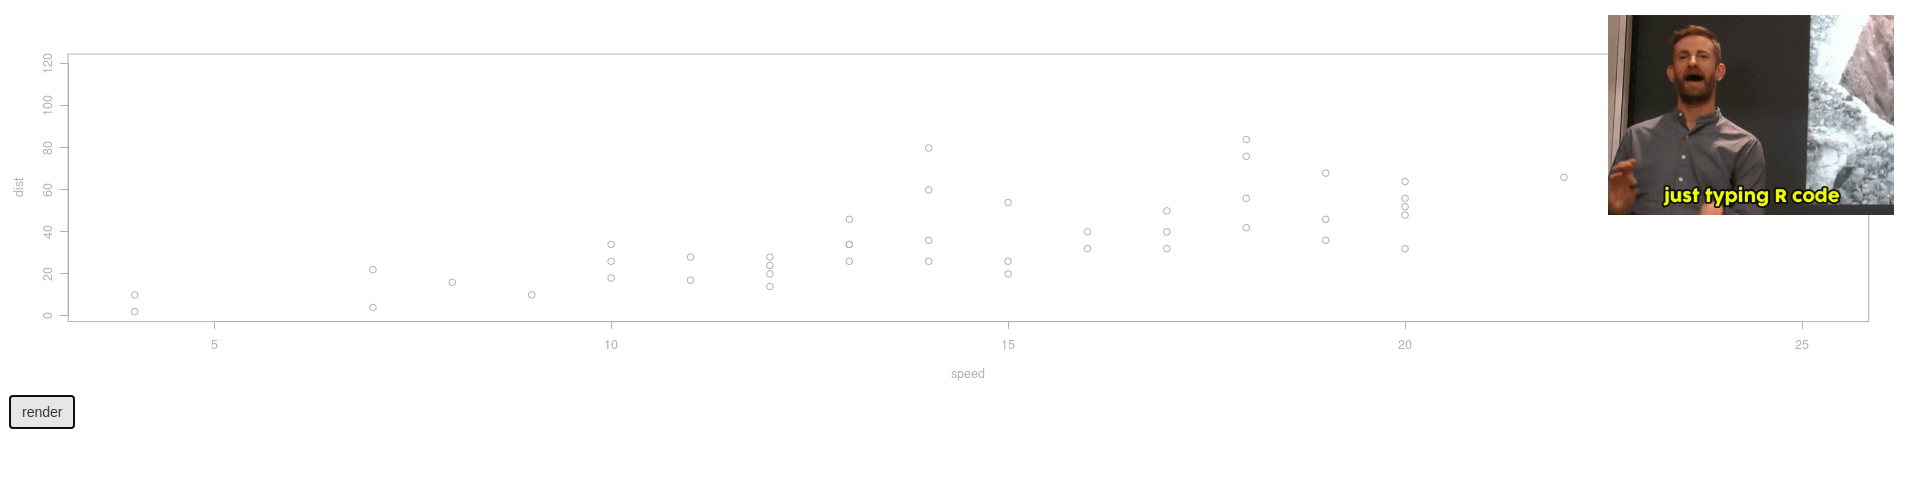
\includegraphics{images/shiny-events.png}
\caption{Shiny with a busy indicator}
\end{figure}

\hypertarget{table-buttons}{%
\section{Table Buttons}\label{table-buttons}}

For instance, using what was learned previously one can place buttons inside a shiny table and observe server-side which is clicked. Starting with a basic application that only includes a table to which we ultimately want to add a column containing a button on each row. Here we achieve this by having each button set a different value (e.g.: an id) to an input using \texttt{shiny.setInputValue} but one could very well create different input names for each button.

\begin{Shaded}
\begin{Highlighting}[]
\KeywordTok{library}\NormalTok{(DT)}
\KeywordTok{library}\NormalTok{(shiny)}

\NormalTok{ui <{-}}\StringTok{ }\KeywordTok{fluidPage}\NormalTok{(}
  \KeywordTok{DTOutput}\NormalTok{(}\StringTok{"table"}\NormalTok{)}
\NormalTok{)}

\NormalTok{server <{-}}\StringTok{ }\ControlFlowTok{function}\NormalTok{(input, output) \{}

\NormalTok{  output}\OperatorTok{$}\NormalTok{table <{-}}\StringTok{ }\KeywordTok{renderDT}\NormalTok{(\{}
    \KeywordTok{datatable}\NormalTok{(}
\NormalTok{      mtcars, }
      \DataTypeTok{escape =} \OtherTok{FALSE}\NormalTok{, }
      \DataTypeTok{selection =} \StringTok{"none"}\NormalTok{, }
      \DataTypeTok{rownames =} \OtherTok{FALSE}\NormalTok{, }
      \DataTypeTok{style =} \StringTok{"bootstrap"}
\NormalTok{    )}
\NormalTok{  \})}

\NormalTok{\}}

\KeywordTok{shinyApp}\NormalTok{(ui, server)}
\end{Highlighting}
\end{Shaded}

Note that in the above we pass some parameters to \texttt{datatable} not all are necessary at the exception of \texttt{escape} which is set to \texttt{FALSE} as we will ultimately place HTML code the table which should appear rendered rather than show said code as a string.

We start by creating the on-click functions as R character strings for each row of the \texttt{mtcars} dataset. This is the function that will be triggered when buttons are clicked. This should look familiar, we use \texttt{Shiny.setInputValue} to define an input named \texttt{click} which is set to a different value for every row of the table.

\begin{Shaded}
\begin{Highlighting}[]
\KeywordTok{library}\NormalTok{(DT)}
\KeywordTok{library}\NormalTok{(shiny)}

\NormalTok{ui <{-}}\StringTok{ }\KeywordTok{fluidPage}\NormalTok{(}
  \KeywordTok{DTOutput}\NormalTok{(}\StringTok{"table"}\NormalTok{)}
\NormalTok{)}

\NormalTok{server <{-}}\StringTok{ }\ControlFlowTok{function}\NormalTok{(input, output) \{}

\NormalTok{  output}\OperatorTok{$}\NormalTok{table <{-}}\StringTok{ }\KeywordTok{renderDT}\NormalTok{(\{}
    \CommentTok{\# on click function}
\NormalTok{    onclick <{-}}\StringTok{ }\KeywordTok{sprintf}\NormalTok{(}
      \StringTok{"Shiny.setInputValue(\textquotesingle{}click\textquotesingle{}, \textquotesingle{}\%s\textquotesingle{})"}\NormalTok{, }
      \KeywordTok{rownames}\NormalTok{(mtcars)}
\NormalTok{    ) }
    
    \KeywordTok{datatable}\NormalTok{(}
\NormalTok{      mtcars, }
      \DataTypeTok{escape =} \OtherTok{FALSE}\NormalTok{, }
      \DataTypeTok{selection =} \StringTok{"none"}\NormalTok{, }
      \DataTypeTok{rownames =} \OtherTok{FALSE}\NormalTok{, }
      \DataTypeTok{style =} \StringTok{"bootstrap"}
\NormalTok{    )}
\NormalTok{  \})}

\NormalTok{\}}

\KeywordTok{shinyApp}\NormalTok{(ui, server)}
\end{Highlighting}
\end{Shaded}

Next we create the buttons for each row and set the JavaScript functions previously created as the \texttt{onClick} attributes. The JavaScript code passed to the \texttt{onClick} attribute will be executed every time the button is clicked.

\begin{Shaded}
\begin{Highlighting}[]
\KeywordTok{library}\NormalTok{(DT)}
\KeywordTok{library}\NormalTok{(shiny)}

\NormalTok{ui <{-}}\StringTok{ }\KeywordTok{fluidPage}\NormalTok{(}
  \KeywordTok{DTOutput}\NormalTok{(}\StringTok{"table"}\NormalTok{)}
\NormalTok{)}

\NormalTok{server <{-}}\StringTok{ }\ControlFlowTok{function}\NormalTok{(input, output) \{}

\NormalTok{  output}\OperatorTok{$}\NormalTok{table <{-}}\StringTok{ }\KeywordTok{renderDT}\NormalTok{(\{}
    \CommentTok{\# on click function}
\NormalTok{    onclick <{-}}\StringTok{ }\KeywordTok{sprintf}\NormalTok{(}
      \StringTok{"Shiny.setInputValue(\textquotesingle{}click\textquotesingle{}, \textquotesingle{}\%s\textquotesingle{})"}\NormalTok{, }
      \KeywordTok{rownames}\NormalTok{(mtcars)}
\NormalTok{    ) }

    \CommentTok{\# button with onClick function}
\NormalTok{    button <{-}}\StringTok{ }\KeywordTok{sprintf}\NormalTok{(}
      \StringTok{"<a class=\textquotesingle{}btn btn{-}primary\textquotesingle{} onClick=\textquotesingle{}\%s\textquotesingle{}>Click me</a>"}\NormalTok{,}
\NormalTok{      onclick}
\NormalTok{    )}

\NormalTok{    mtcars}\OperatorTok{$}\NormalTok{button <{-}}\StringTok{ }\NormalTok{button}
    \KeywordTok{datatable}\NormalTok{(}
\NormalTok{      mtcars, }
      \DataTypeTok{escape =} \OtherTok{FALSE}\NormalTok{, }
      \DataTypeTok{selection =} \StringTok{"none"}\NormalTok{, }
      \DataTypeTok{rownames =} \OtherTok{FALSE}\NormalTok{, }
      \DataTypeTok{style =} \StringTok{"bootstrap"}
\NormalTok{    )}
\NormalTok{  \})}

\NormalTok{\}}

\KeywordTok{shinyApp}\NormalTok{(ui, server)}
\end{Highlighting}
\end{Shaded}

We can then observe the \texttt{click} input and, to demonstrate, render it's value in the UI.

\begin{Shaded}
\begin{Highlighting}[]
\KeywordTok{library}\NormalTok{(DT)}
\KeywordTok{library}\NormalTok{(shiny)}

\NormalTok{ui <{-}}\StringTok{ }\KeywordTok{fluidPage}\NormalTok{(}
  \KeywordTok{br}\NormalTok{(),}
  \KeywordTok{DTOutput}\NormalTok{(}\StringTok{"table"}\NormalTok{),}
  \KeywordTok{strong}\NormalTok{(}\StringTok{"Clicked Model:"}\NormalTok{),}
  \KeywordTok{verbatimTextOutput}\NormalTok{(}\StringTok{"model"}\NormalTok{)}
\NormalTok{)}

\NormalTok{server <{-}}\StringTok{ }\ControlFlowTok{function}\NormalTok{(input, output) \{}

\NormalTok{  output}\OperatorTok{$}\NormalTok{table <{-}}\StringTok{ }\KeywordTok{renderDT}\NormalTok{(\{}
    \CommentTok{\# on click function}
\NormalTok{    onclick <{-}}\StringTok{ }\KeywordTok{sprintf}\NormalTok{(}
      \StringTok{"Shiny.setInputValue(\textquotesingle{}click\textquotesingle{}, \textquotesingle{}\%s\textquotesingle{})"}\NormalTok{, }
      \KeywordTok{rownames}\NormalTok{(mtcars)}
\NormalTok{    ) }

    \CommentTok{\# button with onClick function}
\NormalTok{    button <{-}}\StringTok{ }\KeywordTok{sprintf}\NormalTok{(}
      \StringTok{"<a class=\textquotesingle{}btn btn{-}primary\textquotesingle{} onClick=\textquotesingle{}\%s\textquotesingle{}>Click me</a>"}\NormalTok{,}
\NormalTok{      onclick}
\NormalTok{    )}

    \CommentTok{\# add button to data.frame}
\NormalTok{    mtcars}\OperatorTok{$}\NormalTok{button <{-}}\StringTok{ }\NormalTok{button}

    \KeywordTok{datatable}\NormalTok{(}
\NormalTok{      mtcars, }
      \DataTypeTok{escape =} \OtherTok{FALSE}\NormalTok{, }
      \DataTypeTok{selection =} \StringTok{"none"}\NormalTok{, }
      \DataTypeTok{rownames =} \OtherTok{FALSE}\NormalTok{, }
      \DataTypeTok{style =} \StringTok{"bootstrap"}
\NormalTok{    )}
\NormalTok{  \})}

\NormalTok{  output}\OperatorTok{$}\NormalTok{model <{-}}\StringTok{ }\KeywordTok{renderPrint}\NormalTok{(\{}
    \KeywordTok{print}\NormalTok{(input}\OperatorTok{$}\NormalTok{click)}
\NormalTok{  \})}
\NormalTok{\}}

\KeywordTok{shinyApp}\NormalTok{(ui, server)}
\end{Highlighting}
\end{Shaded}

\begin{figure}
\centering
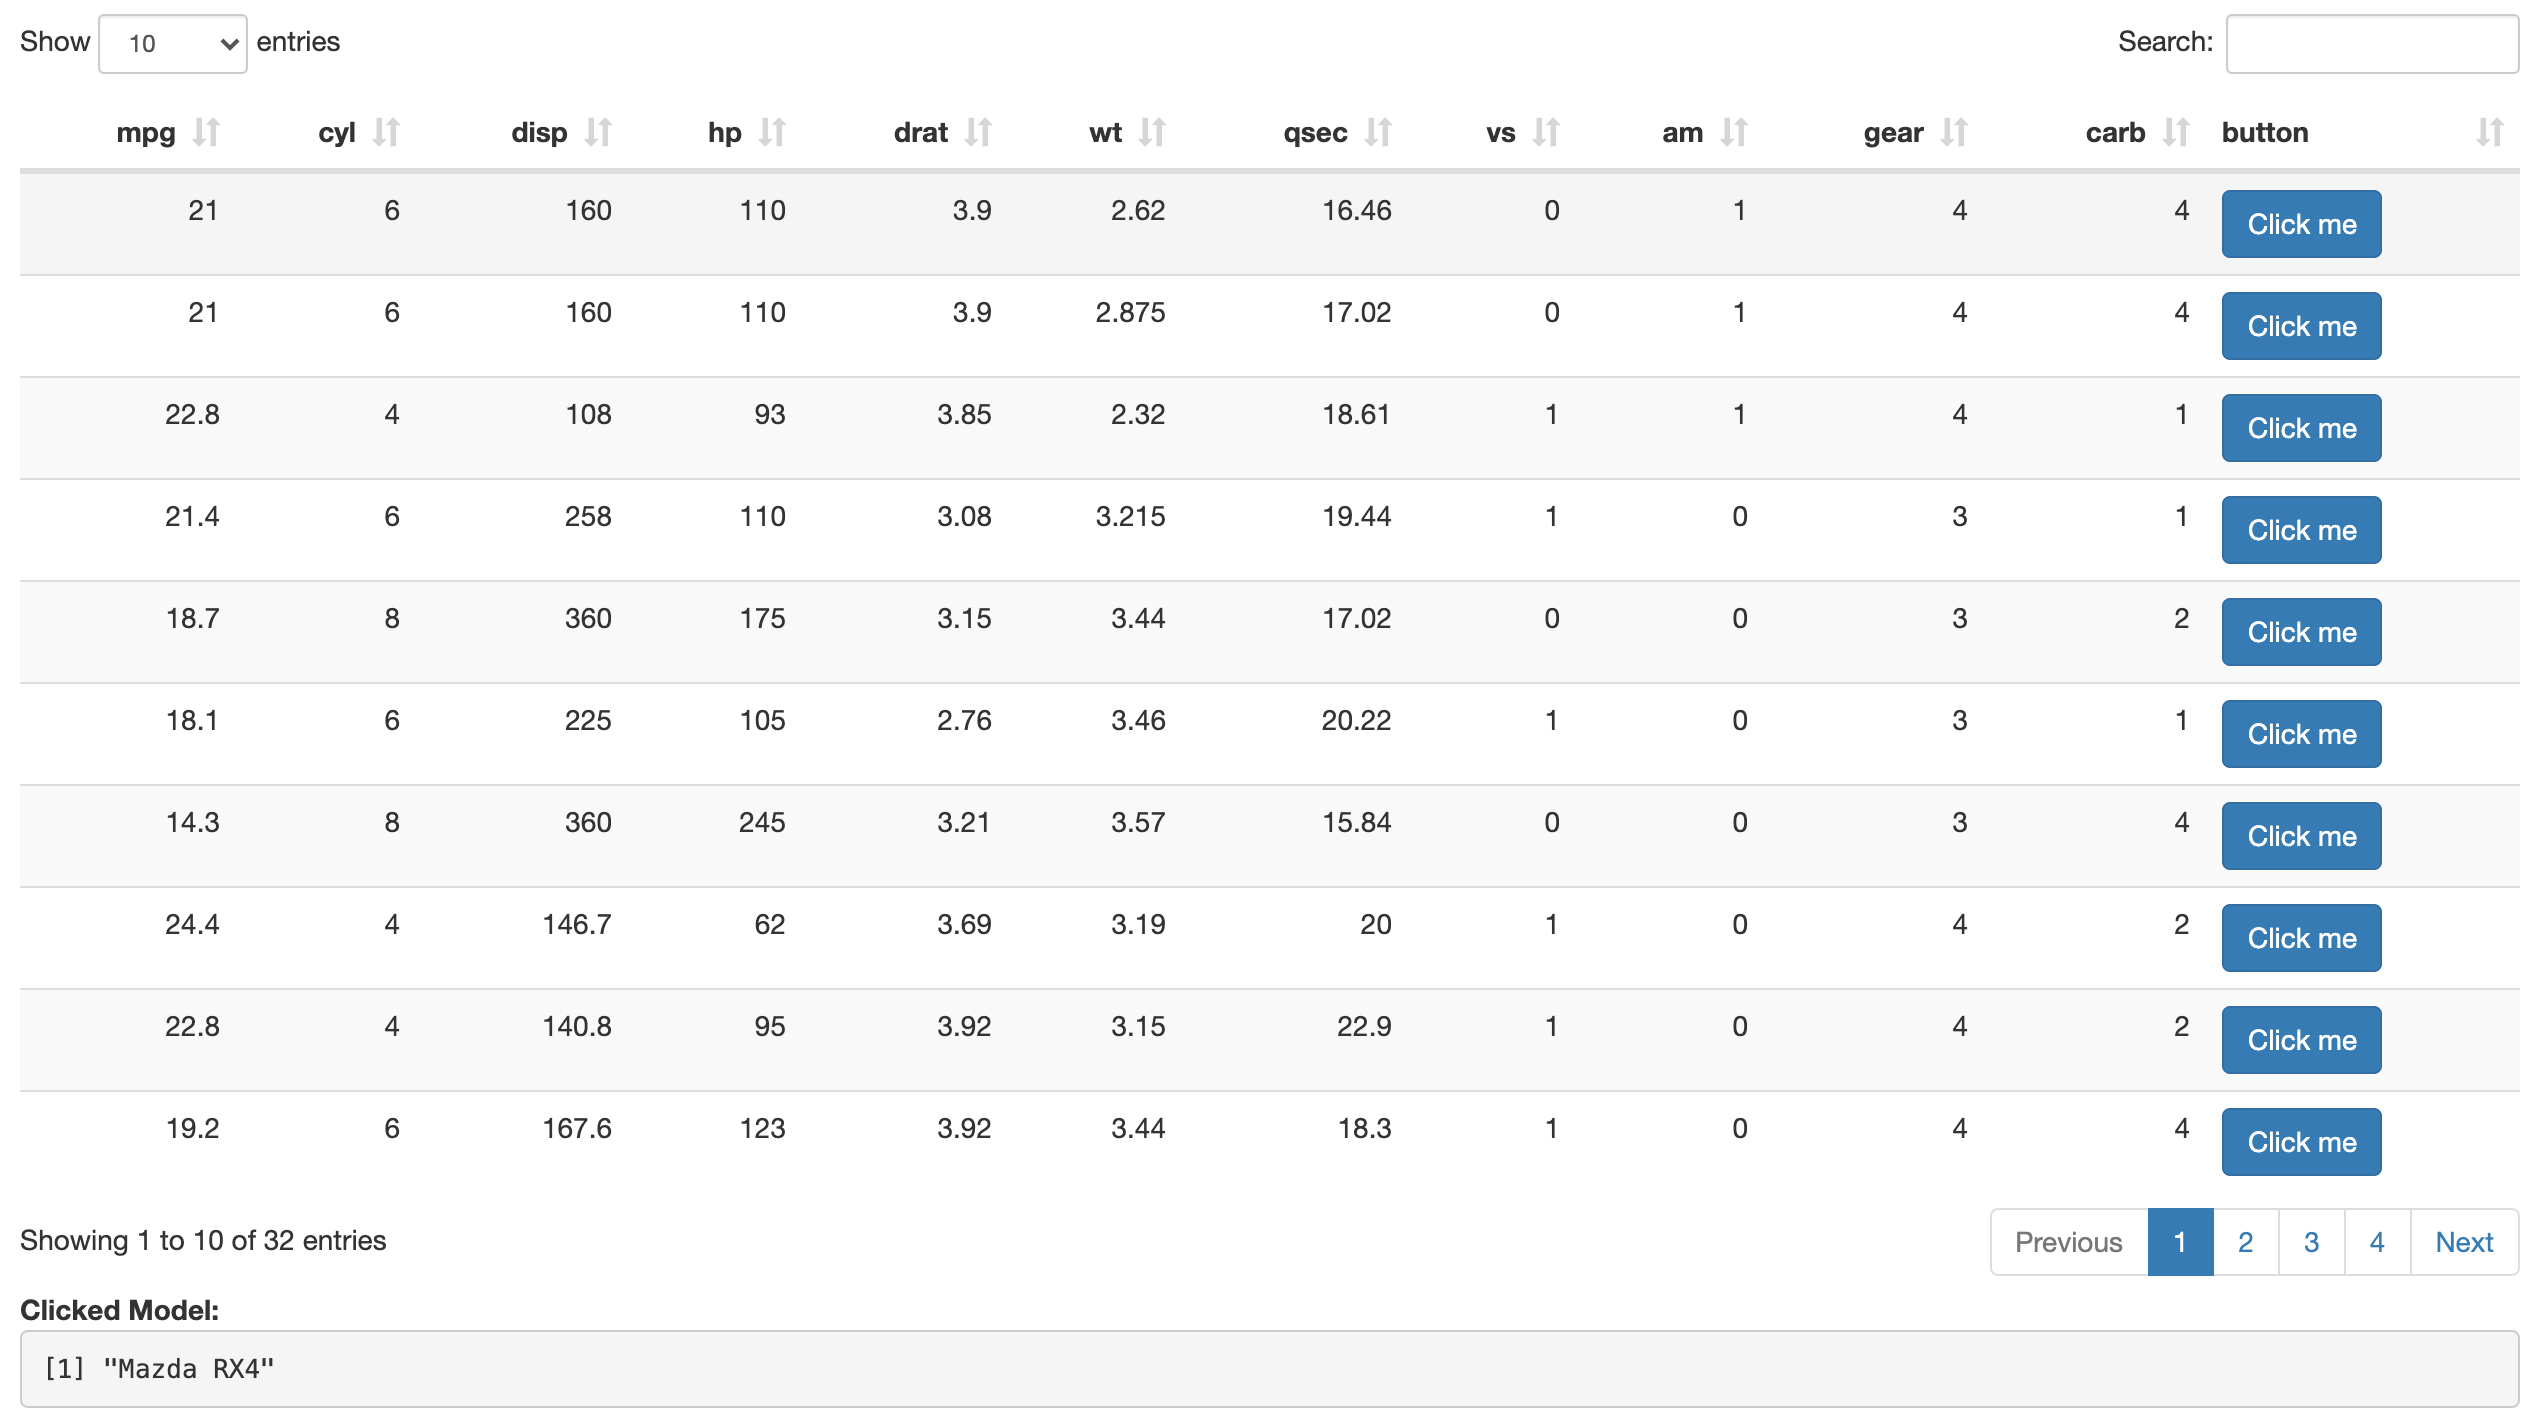
\includegraphics{images/dt-button.png}
\caption{DT with custom input}
\end{figure}

\hypertarget{jquery---toggle}{%
\section{jQuery - Toggle}\label{jquery---toggle}}

The shiny framework itself makes use and thus imports the \href{https://jquery.com/}{jQuery} JavaScript library, a library that provides a convenient API to make a lot of things easier, including animations.

As an example, we could use jQuery's \texttt{show}, \texttt{hide}, or \texttt{toggle} functions to show or hide an HTML element at the press of a button.

\begin{Shaded}
\begin{Highlighting}[]
\CommentTok{// example of jQuery animation}
\AttributeTok{$}\NormalTok{(}\StringTok{\textquotesingle{}\#id\textquotesingle{}}\NormalTok{).}\AttributeTok{toggle}\NormalTok{()}\OperatorTok{;}
\end{Highlighting}
\end{Shaded}

Because jQuery is already imported there is no need to do so, on the contrary, importing it again will impact load time and might clash with the pre-existing version. Below we create a shiny application containing a message handler to toggle (show or hide element depending on its state) at the click of a button.

\begin{Shaded}
\begin{Highlighting}[]
\KeywordTok{library}\NormalTok{(shiny)}

\NormalTok{ui <{-}}\StringTok{ }\KeywordTok{fluidPage}\NormalTok{(}
\NormalTok{  tags}\OperatorTok{$}\KeywordTok{head}\NormalTok{(}
\NormalTok{    tags}\OperatorTok{$}\KeywordTok{script}\NormalTok{(}
      \StringTok{"Shiny.addCustomMessageHandler(}
\StringTok{        \textquotesingle{}jquery{-}toggle\textquotesingle{}, function(id)\{}
\StringTok{          $(\textquotesingle{}\#\textquotesingle{} + id).toggle(); // id}
\StringTok{      \});"}
\NormalTok{    )}
\NormalTok{  ),}
  \KeywordTok{actionButton}\NormalTok{(}\StringTok{"toggle"}\NormalTok{, }\StringTok{"Toggle text"}\NormalTok{),}
  \KeywordTok{h1}\NormalTok{(}\StringTok{"This text is shown!"}\NormalTok{, }\DataTypeTok{id =} \StringTok{"text"}\NormalTok{)}
\NormalTok{)}

\NormalTok{server <{-}}\StringTok{ }\ControlFlowTok{function}\NormalTok{(input, output, session)\{}

  \KeywordTok{observeEvent}\NormalTok{(input}\OperatorTok{$}\NormalTok{toggle, \{}
\NormalTok{    session}\OperatorTok{$}\KeywordTok{sendCustomMessage}\NormalTok{(}\StringTok{\textquotesingle{}jquery{-}toggle\textquotesingle{}}\NormalTok{, }\StringTok{"text"}\NormalTok{)}
\NormalTok{  \})}

\NormalTok{\}}

\KeywordTok{shinyApp}\NormalTok{(ui, server)}
\end{Highlighting}
\end{Shaded}

Note that jQuery takes a selector so one could very well use a class to hide and show multiple elements (with said class) at once.

\begin{Shaded}
\begin{Highlighting}[]
\KeywordTok{library}\NormalTok{(shiny)}

\NormalTok{ui <{-}}\StringTok{ }\KeywordTok{fluidPage}\NormalTok{(}
\NormalTok{  tags}\OperatorTok{$}\KeywordTok{head}\NormalTok{(}
\NormalTok{    tags}\OperatorTok{$}\KeywordTok{script}\NormalTok{(}
      \StringTok{"Shiny.addCustomMessageHandler(}
\StringTok{        \textquotesingle{}jquery{-}toggle\textquotesingle{}, function(selector)\{}
\StringTok{          $(selector).toggle();}
\StringTok{      \});"}
\NormalTok{    )}
\NormalTok{  ),}
  \KeywordTok{actionButton}\NormalTok{(}\StringTok{"toggle"}\NormalTok{, }\StringTok{"Toggle text"}\NormalTok{),}
  \KeywordTok{h1}\NormalTok{(}\StringTok{"This text is shown!"}\NormalTok{, }\DataTypeTok{class =} \StringTok{"to{-}toggle"}\NormalTok{),}
  \KeywordTok{actionButton}\NormalTok{(}\StringTok{"btn"}\NormalTok{, }\StringTok{"Another visible button"}\NormalTok{, }\DataTypeTok{class =} \StringTok{"to{-}toggle"}\NormalTok{)}
\NormalTok{)}

\NormalTok{server <{-}}\StringTok{ }\ControlFlowTok{function}\NormalTok{(input, output, session)\{}

  \KeywordTok{observeEvent}\NormalTok{(input}\OperatorTok{$}\NormalTok{toggle, \{}
\NormalTok{    session}\OperatorTok{$}\KeywordTok{sendCustomMessage}\NormalTok{(}\StringTok{\textquotesingle{}jquery{-}toggle\textquotesingle{}}\NormalTok{, }\StringTok{".to{-}toggle"}\NormalTok{)}
\NormalTok{  \})}

\NormalTok{\}}

\KeywordTok{shinyApp}\NormalTok{(ui, server)}
\end{Highlighting}
\end{Shaded}

This is something where, again, R is leveraged in order to make it easier on the shiny developer but it must be said that it suffers from some inefficiency: the message travels from the browser (button click) to the R server where it is sent back to the browser and triggers \texttt{toggle}. It could indeed very well be rewritten in JavaScript entirely, this is however outside the scope of this book.

\hypertarget{custom-outputs}{%
\chapter{Custom Outputs}\label{custom-outputs}}

In this chapter we create a custom shiny output, in practical terms this creates custom \texttt{render*} and \texttt{*Output} functions to use in Shiny. This will be demonstrated by creating something akin to the \texttt{valueBox} available in the shinydashboard \citep{R-shinydashboard} package. While similar to what shinydashboard provides this box will 1) be fully customisable and 2) available in any shiny application.

The \texttt{valueBox} equivalent we shall build in this chapter is named ``boxxy,'' and allows creating simple but colourful value boxes with animated numbers (by counting up to it) using \href{https://github.com/inorganik/countUp.js}{countUp.js}.

\begin{Shaded}
\begin{Highlighting}[]
\KeywordTok{library}\NormalTok{(shiny)}

\NormalTok{ui <{-}}\StringTok{ }\KeywordTok{fluidPage}\NormalTok{(}
  \KeywordTok{boxxyOutput}\NormalTok{(}\StringTok{"countries"}\NormalTok{)}
\NormalTok{)}

\NormalTok{server <{-}}\StringTok{ }\ControlFlowTok{function}\NormalTok{(input, output)\{}
\NormalTok{  output}\OperatorTok{$}\NormalTok{countries <{-}}\StringTok{ }\KeywordTok{renderBoxxy}\NormalTok{(\{}
    \KeywordTok{boxxy}\NormalTok{(}\StringTok{"Countries"}\NormalTok{, }\DecValTok{95}\NormalTok{)}
\NormalTok{  \})}
\NormalTok{\}}

\KeywordTok{shinyApp}\NormalTok{(ui, server)}
\end{Highlighting}
\end{Shaded}

\begin{figure}
\centering
\includegraphics{images/boxxy-example.png}
\caption{Custom output example}
\end{figure}

\hypertarget{custom-outputs-inner-workings}{%
\section{Custom outputs inner-workings}\label{custom-outputs-inner-workings}}

At the core, this consists in creating three functions; \texttt{boxxy}, \texttt{renderBoxxy} and \texttt{boxxyOutput} (analogous to \texttt{plot}, \texttt{renderPlot}, \texttt{plotOutput}) which are linked by an ``output binding'' in JavaScript.

The first function, \texttt{boxxy} will accept arguments that help define what is in the box. This function is generally useful to preprocess any of the arguments that are meant to produce the custom output. The \texttt{boxxyOutput} function essentially creates the scaffold of the HTML output (e.g.: \texttt{\textless{}div\textgreater{}}) as well as the dependencies. The \texttt{render*} function is perhaps more peculiar it should accept an expression and return a function.

Previous work with shiny and JavaScript covered in this book had no dedicated ``output'' element that were placed in the shiny UI, therefore one had to use a function solely dedicated to importing the dependencies (e.g.: \texttt{usejBox}). However, since this is not the case here the dependencies can be attached together with the output.

Finally, the two R functions are ``bound'' JavaScript-side with an ``output binding'' that renders the data from the \texttt{render*} function with its \texttt{*output}.

\hypertarget{setup}{%
\section{Setup}\label{setup}}

The custom output will be part of a shiny application, let us thus create the basic skeleton of an application and download the dependencies. Create a project in RStudio or an empty directory, then:

\begin{enumerate}
\def\labelenumi{\arabic{enumi}.}
\tightlist
\item
  Create an \texttt{app.R} file that will hold the code for the application and \texttt{boxxy}, \texttt{boxxyOutput}, and \texttt{renderBoxxy} functions
\item
  Create an \texttt{assets} directory that will contain the CSS and JavaScript files.
\item
  Download the countUp.js dependency.
\item
  Create a \texttt{binding.js} JavaScript file for the JavaScript binding within the previously created \texttt{assets} directory.
\item
  Create a \texttt{styles.css} file in the \texttt{assets} directory.
\end{enumerate}

\begin{Shaded}
\begin{Highlighting}[]
\CommentTok{\# application file}
\KeywordTok{file.create}\NormalTok{(}\StringTok{"app.R"}\NormalTok{)}

\CommentTok{\# static file directory}
\KeywordTok{dir.create}\NormalTok{(}\StringTok{"assets"}\NormalTok{)}

\CommentTok{\# countup dependency}
\NormalTok{url <{-}}\StringTok{ }\KeywordTok{paste0}\NormalTok{(}
  \StringTok{"https://cdn.jsdelivr.net/npm/"}\NormalTok{,}
  \StringTok{"countup@1.8.2/countUp.js"}
\NormalTok{)}

\KeywordTok{download.file}\NormalTok{(url, }\StringTok{"assets/countup.js"}\NormalTok{)}

\CommentTok{\# create binding file}
\KeywordTok{file.create}\NormalTok{(}\StringTok{"assets/binding.js"}\NormalTok{)}

\CommentTok{\# CSS file}
\KeywordTok{file.create}\NormalTok{(}\StringTok{"assets/styles.css"}\NormalTok{)}
\end{Highlighting}
\end{Shaded}

This should produce the following directory structure.

\begin{verbatim}
.
├── app.R
└── assets
    ├── binding.js
    ├── countup.js
    └── styles.css
\end{verbatim}

\hypertarget{r-function}{%
\section{R function}\label{r-function}}

The \texttt{boxxy} function takes three arguments, a \texttt{title}, a \texttt{value} that will be animated and the background \texttt{color} to use for the box. The function, at this stage at least, does not preprocess the arguments and simply returns them as a named \texttt{list}.

\begin{Shaded}
\begin{Highlighting}[]
\CommentTok{\# app.R}
\KeywordTok{library}\NormalTok{(shiny)}

\NormalTok{boxxy <{-}}\StringTok{ }\ControlFlowTok{function}\NormalTok{(title, value, }\DataTypeTok{color =} \StringTok{"\#ef476f"}\NormalTok{)\{}
  \KeywordTok{list}\NormalTok{(}\DataTypeTok{title =}\NormalTok{ title, }\DataTypeTok{value =}\NormalTok{ value, }\DataTypeTok{color =}\NormalTok{ color)}
\NormalTok{\}}
\end{Highlighting}
\end{Shaded}

\hypertarget{output}{%
\section{Output}\label{output}}

The \texttt{boxxyOutput} function, like all such functions (\texttt{plotOutput}, \texttt{uiOutput}, etc.) takes an \texttt{id}. This function should return an HTML tag which bears an \texttt{id}, or a \texttt{data-input-id} attribute (more on that later) and a \texttt{class}. The \texttt{id} is to be defined by the user of the function in Shiny just like any other such outputs. For instance, \texttt{plotOutput} creates a \texttt{\textless{}div\textgreater{}} the \texttt{id} of which is actually the \texttt{id} used in the \texttt{plotOutput} function.

\begin{Shaded}
\begin{Highlighting}[]
\CommentTok{\# the id is used as id to the element}
\NormalTok{shiny}\OperatorTok{::}\KeywordTok{plotOutput}\NormalTok{(}\DataTypeTok{id =} \StringTok{"myPlotId"}\NormalTok{)}
\end{Highlighting}
\end{Shaded}

\begin{Shaded}
\begin{Highlighting}[]
\OperatorTok{<}\NormalTok{div }
\NormalTok{  id=}\StringTok{"myPlotId"} 
\NormalTok{  class=}\StringTok{"shiny{-}plot{-}output"} 
\NormalTok{  style=}\StringTok{"width: 100\% ; height: 400px"}\OperatorTok{>}
\ErrorTok{</}\NormalTok{div}\OperatorTok{>}
\end{Highlighting}
\end{Shaded}

The \texttt{class} is used JavaScript-side to ``find'' the outputs in the DOM (document object model) and generate the output. The function \texttt{boxxyOutput} could thus be as shown below, the \texttt{id} is passed along to the \texttt{\textless{}div\textgreater{}} which is created with a \texttt{boxxy} class that will be used in the output binding to find that element and generate the output within that very \texttt{\textless{}div\textgreater{}} using data that will be passed from the server.

\begin{Shaded}
\begin{Highlighting}[]
\NormalTok{boxxyOutput <{-}}\StringTok{ }\ControlFlowTok{function}\NormalTok{(id)\{}
  \CommentTok{\# the HTML output}
\NormalTok{  shiny}\OperatorTok{::}\NormalTok{tags}\OperatorTok{$}\KeywordTok{div}\NormalTok{(}
    \DataTypeTok{id =}\NormalTok{ id, }\DataTypeTok{class =} \StringTok{"boxxy"}
\NormalTok{  )}
\NormalTok{\}}
\end{Highlighting}
\end{Shaded}

\begin{rmdnote}
Make sure you use unique class names so they are not accidentally
overridden by the user.
\end{rmdnote}

As shown previously the box should include a title and an animated value. These could be generated entirely in JavaScript but it's actually easier to create placeholders with htmltools tags, we generate dynamic ids for those so they can easily be referenced later on in JavaScript: \texttt{id-boxxy-value} for the value and \texttt{id-boxxy-title} for the title.

\begin{Shaded}
\begin{Highlighting}[]
\NormalTok{boxxyOutput <{-}}\StringTok{ }\ControlFlowTok{function}\NormalTok{(id)\{}
  \CommentTok{\# the HTML output}
\NormalTok{  shiny}\OperatorTok{::}\NormalTok{tags}\OperatorTok{$}\KeywordTok{div}\NormalTok{(}
    \DataTypeTok{id =}\NormalTok{ id, }\DataTypeTok{class =} \StringTok{"boxxy"}\NormalTok{,}
    \KeywordTok{h1}\NormalTok{(}
      \DataTypeTok{id =} \KeywordTok{sprintf}\NormalTok{(}\StringTok{"\%s{-}boxxy{-}value"}\NormalTok{, id), }
      \DataTypeTok{class =} \StringTok{"boxxy{-}value"}
\NormalTok{    ),}
    \KeywordTok{p}\NormalTok{(}
      \DataTypeTok{id =} \KeywordTok{sprintf}\NormalTok{(}\StringTok{"\%s{-}boxxy{-}title"}\NormalTok{, id), }
      \DataTypeTok{class =} \StringTok{"boxxy{-}title"}
\NormalTok{    )}
\NormalTok{  )}
\NormalTok{\}}
\end{Highlighting}
\end{Shaded}

Finally, we also used classes in the output so every element it comprises can be styled with ease.

\begin{Shaded}
\begin{Highlighting}[]
\FunctionTok{.boxxy}\NormalTok{\{}
  \KeywordTok{text{-}align}\NormalTok{: }\DecValTok{center}\OperatorTok{;}
  \KeywordTok{border{-}left}\NormalTok{: }\DecValTok{6}\DataTypeTok{px} \DecValTok{solid} \ConstantTok{\#073b4c}\OperatorTok{;}
  \KeywordTok{padding}\NormalTok{: }\DecValTok{1}\DataTypeTok{em}\OperatorTok{;}
\NormalTok{\}}

\FunctionTok{.boxxy{-}title}\NormalTok{\{}
  \KeywordTok{text{-}transform}\NormalTok{: }\DecValTok{uppercase}\OperatorTok{;}
\NormalTok{\}}

\FunctionTok{.boxxy{-}value}\NormalTok{\{}
  \KeywordTok{font{-}size}\NormalTok{: }\DecValTok{3}\DataTypeTok{em}\OperatorTok{;}
\NormalTok{\}}
\end{Highlighting}
\end{Shaded}

The dependencies should be added to the above, since this function must be placed in the UI for anything to work the dependencies can piggyback on the output element. This works using the htmltools package. The function \texttt{htmltools::htmlDependency} is used to create a dependency that is then attached with \texttt{htmltools::attachDependencies}. While the former creates an object that shiny can understand and translate into \texttt{\textless{}script\textgreater{}} or \texttt{\textless{}style\textgreater{}} tags, the former attaches them to the output object and ensures dependencies are not imported multiple times (e.g.: when \texttt{boxxyOutput} is used more than once).

Notice the use of \texttt{normalizePath} to retrieve the full path to the \texttt{assets} directory as this will not work with a relative path (e.g.: \texttt{./assets}). The dependencies consist of the three files previously created and necessary to generate the output: \texttt{countup.js} the dependency that was downloaded as well as \texttt{binding.js} and \texttt{styles.css}.

\begin{Shaded}
\begin{Highlighting}[]
\NormalTok{boxxyOutput <{-}}\StringTok{ }\ControlFlowTok{function}\NormalTok{(id)\{}
\NormalTok{  el <{-}}\StringTok{ }\NormalTok{tags}\OperatorTok{$}\KeywordTok{div}\NormalTok{(}
    \DataTypeTok{id =}\NormalTok{ id, }\DataTypeTok{class =} \StringTok{"boxxy"}\NormalTok{,}
    \KeywordTok{h1}\NormalTok{(}
      \DataTypeTok{id =} \KeywordTok{sprintf}\NormalTok{(}\StringTok{"\%s{-}boxxy{-}counter"}\NormalTok{, id), }
      \DataTypeTok{class =} \StringTok{"boxxy{-}value"}
\NormalTok{    ),}
    \KeywordTok{p}\NormalTok{(}
      \DataTypeTok{id =} \KeywordTok{sprintf}\NormalTok{(}\StringTok{"\%s{-}boxxy{-}title"}\NormalTok{, id), }
      \DataTypeTok{class =} \StringTok{"boxxy{-}title"}
\NormalTok{    )}
\NormalTok{  )}

  \CommentTok{\# get full path}
\NormalTok{  path <{-}}\StringTok{ }\KeywordTok{normalizePath}\NormalTok{(}\StringTok{"assets"}\NormalTok{)}

\NormalTok{  deps <{-}}\StringTok{ }\KeywordTok{list}\NormalTok{(}
\NormalTok{    htmltools}\OperatorTok{::}\KeywordTok{htmlDependency}\NormalTok{(}
      \DataTypeTok{name =} \StringTok{"boxxy"}\NormalTok{,}
      \DataTypeTok{version =} \StringTok{"1.0.0"}\NormalTok{,}
      \DataTypeTok{src =} \KeywordTok{c}\NormalTok{(}\DataTypeTok{file =}\NormalTok{ path),}
      \DataTypeTok{script =} \KeywordTok{c}\NormalTok{(}\StringTok{"countup.js"}\NormalTok{, }\StringTok{"binding.js"}\NormalTok{),}
      \DataTypeTok{stylesheet =} \StringTok{"styles.css"}
\NormalTok{    )}
\NormalTok{  )}

\NormalTok{  htmltools}\OperatorTok{::}\KeywordTok{attachDependencies}\NormalTok{(el, deps)}
\NormalTok{\}}
\end{Highlighting}
\end{Shaded}

Running the function reveals the HTML it generates at the exception of the dependencies which htmltools does not print to the console.

\begin{Shaded}
\begin{Highlighting}[]
\KeywordTok{boxxyOutput}\NormalTok{(}\StringTok{"myID"}\NormalTok{)}
\end{Highlighting}
\end{Shaded}

\begin{Shaded}
\begin{Highlighting}[]
\KeywordTok{<div}\OtherTok{ id=}\StringTok{"myID"}\OtherTok{ class=}\StringTok{"boxxy"}\KeywordTok{>}
  \KeywordTok{<h1}\OtherTok{ id=}\StringTok{"myID{-}boxxy{-}counter"}\OtherTok{ class=}\StringTok{"boxxy{-}value"}\KeywordTok{></h1>}
  \KeywordTok{<p}\OtherTok{ id=}\StringTok{"myID{-}boxxy{-}title"}\OtherTok{ class=}\StringTok{"boxxy{-}title"}\KeywordTok{></p>}
\KeywordTok{</div>}
\end{Highlighting}
\end{Shaded}

\hypertarget{render}{%
\section{Render}\label{render}}

The function \texttt{renderBoxxy} should accept an expression, like other such \texttt{render*} function. For instance in the example below the \texttt{renderPlot} function does accept an expression which uses, amongst other functions, \texttt{plot}.

\begin{Shaded}
\begin{Highlighting}[]
\NormalTok{output}\OperatorTok{$}\NormalTok{myPlot <{-}}\StringTok{ }\KeywordTok{renderPlot}\NormalTok{(\{}
  \CommentTok{\# this is an expression}
\NormalTok{  cars }\OperatorTok{\%>\%}\StringTok{ }
\StringTok{    }\KeywordTok{head}\NormalTok{() }\OperatorTok{\%>\%}\StringTok{ }
\StringTok{    }\KeywordTok{plot}\NormalTok{()}
\NormalTok{\})}
\end{Highlighting}
\end{Shaded}

The function \texttt{renderBoxxy} takes an expression and other arguments that are passed to \texttt{shiny::exprToFunction} this does pretty much what it says on the tin: it returns a function from an expression (unless that expression is a function, in which case it returns the expression). This function must be further wrapped in another as render functions must return functions.

\begin{Shaded}
\begin{Highlighting}[]
\NormalTok{renderBoxxy <{-}}\StringTok{ }\ControlFlowTok{function}\NormalTok{(expr, }\DataTypeTok{env =} \KeywordTok{parent.frame}\NormalTok{(), }
  \DataTypeTok{quoted =} \OtherTok{FALSE}\NormalTok{) \{}
  \CommentTok{\# Convert the expression + environment into a function}
\NormalTok{  func <{-}}\StringTok{ }\NormalTok{shiny}\OperatorTok{::}\KeywordTok{exprToFunction}\NormalTok{(expr, env, quoted)}

  \ControlFlowTok{function}\NormalTok{()\{}
    \KeywordTok{func}\NormalTok{()}
\NormalTok{  \}}
\NormalTok{\}}
\end{Highlighting}
\end{Shaded}

\hypertarget{javascript-output-binding}{%
\section{JavaScript output binding}\label{javascript-output-binding}}

Here we create an ``output binding,'' it tells Shiny how to find the component and how to interact with it. An output binding is initialised from \texttt{Shiny.OutputBinding}. Below we initialise a new binding.

\begin{Shaded}
\begin{Highlighting}[]
\CommentTok{// custom.js}
\KeywordTok{var}\NormalTok{ boxxyBinding }\OperatorTok{=} \KeywordTok{new} \VariableTok{Shiny}\NormalTok{.}\AttributeTok{OutputBinding}\NormalTok{()}\OperatorTok{;}
\end{Highlighting}
\end{Shaded}

Then, this must be ``extended'' by specifying a number of methods, a very necessary one being \texttt{find}. It is used to look for the output HTML element in the document (\texttt{scope}), and return them as an array (\texttt{HTMLcollection}). Other methods all take an \texttt{el} argument; that value will always be an element that was returned from \texttt{find}. A very straightforward way to accomplish this is to use jQuery's find method to identify elements with the \texttt{boxxy} class used in \texttt{boxxyOutput}. You are by no means forced to use a CSS class to identify the elements but there is no reason not to.

\begin{Shaded}
\begin{Highlighting}[]
\CommentTok{// custom.js}
\KeywordTok{var}\NormalTok{ boxxyBinding }\OperatorTok{=} \KeywordTok{new} \VariableTok{Shiny}\NormalTok{.}\AttributeTok{OutputBinding}\NormalTok{()}\OperatorTok{;}

\VariableTok{$}\NormalTok{.}\AttributeTok{extend}\NormalTok{(boxxyBinding}\OperatorTok{,} \OperatorTok{\{}
  \DataTypeTok{find}\OperatorTok{:} \KeywordTok{function}\NormalTok{(scope) }\OperatorTok{\{}
    \ControlFlowTok{return} \AttributeTok{$}\NormalTok{(scope).}\AttributeTok{find}\NormalTok{(}\StringTok{".boxxy"}\NormalTok{)}\OperatorTok{;}
  \OperatorTok{\}}
\OperatorTok{\}}\NormalTok{)}\OperatorTok{;}
\end{Highlighting}
\end{Shaded}

One might then want to use the \texttt{getId} method which returns the \texttt{id} of the element, by default, as can be seen in the \href{https://github.com/rstudio/shiny/blob/master/srcjs/output_binding.js}{source code} (below), the binding returns the id as the \texttt{data-input-id} attribute and if that is falsy it returns the element's \texttt{id}.

\begin{Shaded}
\begin{Highlighting}[]
\CommentTok{// getId default}
\KeywordTok{this}\NormalTok{.}\AttributeTok{getId} \OperatorTok{=} \KeywordTok{function}\NormalTok{(el) }\OperatorTok{\{}
  \ControlFlowTok{return}\NormalTok{ el[}\StringTok{\textquotesingle{}data{-}input{-}id\textquotesingle{}}\NormalTok{] }\OperatorTok{||} \VariableTok{el}\NormalTok{.}\AttributeTok{id}\OperatorTok{;}
\OperatorTok{\}}
\end{Highlighting}
\end{Shaded}

Since boxxy uses the element id the default will work and this can be skipped entirely.

Next, one needs to implement the \texttt{renderValue} function which is the very function that generates the output based on data used in \texttt{boxxy} and sent to the front-end with \texttt{renderBoxxy}. The \texttt{renderValue} method accepts two arguments, first \texttt{el} the element where the output should be generated, this is effectively the output of \texttt{boxxyOutput} which the binding found using \texttt{find}, the second argument is \texttt{data} which is the data passed to \texttt{boxxy} and serialised via \texttt{renderBoxxy}.

\begin{rmdnote}
The \texttt{renderValue} is in effect very similar if not identical to
the JavaScript function of the same name involved in creating
htmlwidgets.
\end{rmdnote}

\hypertarget{boxxy-title}{%
\subsection{Boxxy title}\label{boxxy-title}}

Let's now tackle the first of the three core aspect of the boxxy output: the title. The \texttt{title} should be placed in the previously created placeholder which bears the \texttt{id-boxxy-title}; exactly as was done with htmlwidgets previously we insert title (\texttt{data.title}) in the element with \texttt{innerText}. The dynamically generated id for the title is built in the same way it is in R, by concatenating the \texttt{id} with \texttt{-boxxy-title}

\begin{itemize}
\tightlist
\item
  In R \texttt{sprintf("\%s-boxxy-title",\ id)}
\item
  In JavaScript \texttt{el.id\ +\ \textquotesingle{}-boxxy-title\textquotesingle{}}
\end{itemize}

\begin{Shaded}
\begin{Highlighting}[]
\KeywordTok{var}\NormalTok{ boxxyBinding }\OperatorTok{=} \KeywordTok{new} \VariableTok{Shiny}\NormalTok{.}\AttributeTok{OutputBinding}\NormalTok{()}\OperatorTok{;}

\VariableTok{$}\NormalTok{.}\AttributeTok{extend}\NormalTok{(boxxyBinding}\OperatorTok{,} \OperatorTok{\{}
  \DataTypeTok{find}\OperatorTok{:} \KeywordTok{function}\NormalTok{(scope) }\OperatorTok{\{}
    \ControlFlowTok{return} \AttributeTok{$}\NormalTok{(scope).}\AttributeTok{find}\NormalTok{(}\StringTok{".boxxy"}\NormalTok{)}\OperatorTok{;}
  \OperatorTok{\},}
  \DataTypeTok{renderValue}\OperatorTok{:} \KeywordTok{function}\NormalTok{(el}\OperatorTok{,}\NormalTok{ data) }\OperatorTok{\{}

    \CommentTok{// insert the title}
    \KeywordTok{let}\NormalTok{ title\_id }\OperatorTok{=} \VariableTok{el}\NormalTok{.}\AttributeTok{id} \OperatorTok{+} \StringTok{\textquotesingle{}{-}boxxy{-}title\textquotesingle{}}\OperatorTok{;}
    \VariableTok{document}\NormalTok{.}\AttributeTok{getElementById}\NormalTok{(title\_id).}\AttributeTok{innerText} \OperatorTok{=} \VariableTok{data}\NormalTok{.}\AttributeTok{title}
  \OperatorTok{\}}
\OperatorTok{\}}\NormalTok{)}\OperatorTok{;}
\end{Highlighting}
\end{Shaded}

\hypertarget{boxxy-value}{%
\subsection{Boxxy value}\label{boxxy-value}}

Though the custom output could be limited to a static value generated in a fashion similar to how the title is placed, we opted for a more fancy animated value using countUp.js.

Initialise a new counter, specifying the id of the element where it should be created, then as second argument the starting value from which the counter should start and finally the value to count up to. Note that there is a fourth argument to pass a JSON of options which we do not use here.

\begin{Shaded}
\begin{Highlighting}[]
\CommentTok{// place counter in elementId}
\CommentTok{// start at 0 and count up to 123}
\KeywordTok{const}\NormalTok{ counter }\OperatorTok{=} \KeywordTok{new} \AttributeTok{CountUp}\NormalTok{(}\StringTok{\textquotesingle{}elementId\textquotesingle{}}\OperatorTok{,} \DecValTok{0}\OperatorTok{,} \DecValTok{123}\NormalTok{)}\OperatorTok{;}
\VariableTok{counter}\NormalTok{.}\AttributeTok{start}\NormalTok{()}\OperatorTok{;}
\end{Highlighting}
\end{Shaded}

The counter has to be generated in the \texttt{\textless{}h1\textgreater{}} placeholder bearing the \texttt{id-boxxy-value}, while the value to count up to is stored in \texttt{data.value} meaning the counter can be initialised with \texttt{new\ CountUp(el.id\ +\ \textquotesingle{}-boxxy-value\textquotesingle{},\ 0,\ data.value);}.

\begin{Shaded}
\begin{Highlighting}[]
\KeywordTok{var}\NormalTok{ boxxyBinding }\OperatorTok{=} \KeywordTok{new} \VariableTok{Shiny}\NormalTok{.}\AttributeTok{OutputBinding}\NormalTok{()}\OperatorTok{;}

\VariableTok{$}\NormalTok{.}\AttributeTok{extend}\NormalTok{(boxxyBinding}\OperatorTok{,} \OperatorTok{\{}
  \DataTypeTok{find}\OperatorTok{:} \KeywordTok{function}\NormalTok{(scope) }\OperatorTok{\{}
    \ControlFlowTok{return} \AttributeTok{$}\NormalTok{(scope).}\AttributeTok{find}\NormalTok{(}\StringTok{".boxxy"}\NormalTok{)}\OperatorTok{;}
  \OperatorTok{\},}
  \DataTypeTok{renderValue}\OperatorTok{:} \KeywordTok{function}\NormalTok{(el}\OperatorTok{,}\NormalTok{ data) }\OperatorTok{\{}

    \CommentTok{// insert the title}
    \KeywordTok{let}\NormalTok{ title\_id }\OperatorTok{=} \VariableTok{el}\NormalTok{.}\AttributeTok{id} \OperatorTok{+} \StringTok{\textquotesingle{}{-}boxxy{-}title\textquotesingle{}}\OperatorTok{;}
    \VariableTok{document}\NormalTok{.}\AttributeTok{getElementById}\NormalTok{(title\_id).}\AttributeTok{innerText} \OperatorTok{=} \VariableTok{data}\NormalTok{.}\AttributeTok{title}

    \CommentTok{// counter start at 0}
    \KeywordTok{let}\NormalTok{ counter\_id }\OperatorTok{=} \VariableTok{el}\NormalTok{.}\AttributeTok{id} \OperatorTok{+} \StringTok{\textquotesingle{}{-}boxxy{-}value\textquotesingle{}}\OperatorTok{;}
    \KeywordTok{var}\NormalTok{ counter }\OperatorTok{=} \KeywordTok{new} \AttributeTok{CountUp}\NormalTok{(counter\_id}\OperatorTok{,} \DecValTok{0}\OperatorTok{,} \VariableTok{data}\NormalTok{.}\AttributeTok{value}\NormalTok{)}\OperatorTok{;}
    \VariableTok{counter}\NormalTok{.}\AttributeTok{start}\NormalTok{()}\OperatorTok{;}
  \OperatorTok{\}}
\OperatorTok{\}}\NormalTok{)}\OperatorTok{;}
\end{Highlighting}
\end{Shaded}

\hypertarget{background-color}{%
\section{Background color}\label{background-color}}

Then we can set the background color that was passed to \texttt{boxxy} (\texttt{data.color}).

\begin{Shaded}
\begin{Highlighting}[]
\KeywordTok{var}\NormalTok{ boxxyBinding }\OperatorTok{=} \KeywordTok{new} \VariableTok{Shiny}\NormalTok{.}\AttributeTok{OutputBinding}\NormalTok{()}\OperatorTok{;}

\VariableTok{$}\NormalTok{.}\AttributeTok{extend}\NormalTok{(boxxyBinding}\OperatorTok{,} \OperatorTok{\{}
  \DataTypeTok{find}\OperatorTok{:} \KeywordTok{function}\NormalTok{(scope) }\OperatorTok{\{}
    \ControlFlowTok{return} \AttributeTok{$}\NormalTok{(scope).}\AttributeTok{find}\NormalTok{(}\StringTok{".boxxy"}\NormalTok{)}\OperatorTok{;}
  \OperatorTok{\},}
  \DataTypeTok{renderValue}\OperatorTok{:} \KeywordTok{function}\NormalTok{(el}\OperatorTok{,}\NormalTok{ data) }\OperatorTok{\{}

    \CommentTok{// insert the title}
    \KeywordTok{let}\NormalTok{ title\_id }\OperatorTok{=} \VariableTok{el}\NormalTok{.}\AttributeTok{id} \OperatorTok{+} \StringTok{\textquotesingle{}{-}boxxy{-}title\textquotesingle{}}\OperatorTok{;}
    \VariableTok{document}\NormalTok{.}\AttributeTok{getElementById}\NormalTok{(title\_id).}\AttributeTok{innerText} \OperatorTok{=} \VariableTok{data}\NormalTok{.}\AttributeTok{title}

    \CommentTok{// counter start at 0}
    \KeywordTok{let}\NormalTok{ counter\_id }\OperatorTok{=} \VariableTok{el}\NormalTok{.}\AttributeTok{id} \OperatorTok{+} \StringTok{\textquotesingle{}{-}boxxy{-}value\textquotesingle{}}\OperatorTok{;}
    \KeywordTok{var}\NormalTok{ counter }\OperatorTok{=} \KeywordTok{new} \AttributeTok{CountUp}\NormalTok{(counter\_id}\OperatorTok{,} \DecValTok{0}\OperatorTok{,} \VariableTok{data}\NormalTok{.}\AttributeTok{value}\NormalTok{)}\OperatorTok{;}
    \VariableTok{counter}\NormalTok{.}\AttributeTok{start}\NormalTok{()}\OperatorTok{;}

    \CommentTok{// background color }
    \VariableTok{el}\NormalTok{.}\VariableTok{style}\NormalTok{.}\AttributeTok{backgroundColor} \OperatorTok{=} \VariableTok{data}\NormalTok{.}\AttributeTok{color}\OperatorTok{;}
  \OperatorTok{\}}
\OperatorTok{\}}\NormalTok{)}\OperatorTok{;}
\end{Highlighting}
\end{Shaded}

\hypertarget{register-the-output-binding}{%
\subsection{Register the output binding}\label{register-the-output-binding}}

Finally, the output binding must be registered with shiny. Note that it uses a unique string identifier, the \href{https://shiny.rstudio.com/articles/building-outputs.html}{documentation} states:

\begin{quote}
At the moment it is unused but future features may depend on it.
\end{quote}

\begin{Shaded}
\begin{Highlighting}[]
\KeywordTok{var}\NormalTok{ boxxyBinding }\OperatorTok{=} \KeywordTok{new} \VariableTok{Shiny}\NormalTok{.}\AttributeTok{OutputBinding}\NormalTok{()}\OperatorTok{;}

\VariableTok{$}\NormalTok{.}\AttributeTok{extend}\NormalTok{(boxxyBinding}\OperatorTok{,} \OperatorTok{\{}
  \DataTypeTok{find}\OperatorTok{:} \KeywordTok{function}\NormalTok{(scope) }\OperatorTok{\{}
    \ControlFlowTok{return} \AttributeTok{$}\NormalTok{(scope).}\AttributeTok{find}\NormalTok{(}\StringTok{".boxxy"}\NormalTok{)}\OperatorTok{;}
  \OperatorTok{\},}
  \DataTypeTok{renderValue}\OperatorTok{:} \KeywordTok{function}\NormalTok{(el}\OperatorTok{,}\NormalTok{ data) }\OperatorTok{\{}

    \CommentTok{// insert the title}
    \KeywordTok{let}\NormalTok{ title\_id }\OperatorTok{=} \VariableTok{el}\NormalTok{.}\AttributeTok{id} \OperatorTok{+} \StringTok{\textquotesingle{}{-}boxxy{-}title\textquotesingle{}}\OperatorTok{;}
    \VariableTok{document}\NormalTok{.}\AttributeTok{getElementById}\NormalTok{(title\_id).}\AttributeTok{innerText} \OperatorTok{=} \VariableTok{data}\NormalTok{.}\AttributeTok{title}

    \CommentTok{// counter start at 0}
    \KeywordTok{let}\NormalTok{ counter\_id }\OperatorTok{=} \VariableTok{el}\NormalTok{.}\AttributeTok{id} \OperatorTok{+} \StringTok{\textquotesingle{}{-}boxxy{-}value\textquotesingle{}}\OperatorTok{;}
    \KeywordTok{var}\NormalTok{ counter }\OperatorTok{=} \KeywordTok{new} \AttributeTok{CountUp}\NormalTok{(counter\_id}\OperatorTok{,} \DecValTok{0}\OperatorTok{,} \VariableTok{data}\NormalTok{.}\AttributeTok{value}\NormalTok{)}\OperatorTok{;}
    \VariableTok{counter}\NormalTok{.}\AttributeTok{start}\NormalTok{()}\OperatorTok{;}

    \CommentTok{// background color }
    \VariableTok{el}\NormalTok{.}\VariableTok{style}\NormalTok{.}\AttributeTok{backgroundColor} \OperatorTok{=} \VariableTok{data}\NormalTok{.}\AttributeTok{color}\OperatorTok{;}
  \OperatorTok{\}}
\OperatorTok{\}}\NormalTok{)}\OperatorTok{;}

\CommentTok{// register}
\VariableTok{Shiny}\NormalTok{.}\VariableTok{outputBindings}\NormalTok{.}\AttributeTok{register}\NormalTok{(boxxyBinding}\OperatorTok{,} \StringTok{"john.boxxy"}\NormalTok{)}\OperatorTok{;}
\end{Highlighting}
\end{Shaded}

Ensure that string uniquely identifies the binding to avoid future clash with other such bindings.

\hypertarget{boxxy-usage}{%
\section{Boxxy usage}\label{boxxy-usage}}

With all of this in place one can use boxxy in a shiny application.

\begin{Shaded}
\begin{Highlighting}[]
\KeywordTok{library}\NormalTok{(shiny)}

\NormalTok{boxxy <{-}}\StringTok{ }\ControlFlowTok{function}\NormalTok{(title, value, }\DataTypeTok{color =} \StringTok{"black"}\NormalTok{)\{}
  \KeywordTok{list}\NormalTok{(}\DataTypeTok{title =}\NormalTok{ title, }\DataTypeTok{value =}\NormalTok{ value, }\DataTypeTok{color =}\NormalTok{ color)}
\NormalTok{\}}

\NormalTok{boxxyOutput <{-}}\StringTok{ }\ControlFlowTok{function}\NormalTok{(id)\{}
\NormalTok{  el <{-}}\StringTok{ }\NormalTok{shiny}\OperatorTok{::}\NormalTok{tags}\OperatorTok{$}\KeywordTok{div}\NormalTok{(}
    \DataTypeTok{id =}\NormalTok{ id, }\DataTypeTok{class =} \StringTok{"boxxy"}\NormalTok{,}
    \KeywordTok{h1}\NormalTok{(}\DataTypeTok{id =} \KeywordTok{sprintf}\NormalTok{(}\StringTok{"\%s{-}boxxy{-}value"}\NormalTok{, id), }\DataTypeTok{class =} \StringTok{"boxxy{-}value"}\NormalTok{),}
    \KeywordTok{p}\NormalTok{(}\DataTypeTok{id =} \KeywordTok{sprintf}\NormalTok{(}\StringTok{"\%s{-}boxxy{-}title"}\NormalTok{, id), }\DataTypeTok{class =} \StringTok{"boxxy{-}title"}\NormalTok{)}
\NormalTok{  )}

\NormalTok{  path <{-}}\StringTok{ }\KeywordTok{normalizePath}\NormalTok{(}\StringTok{"assets"}\NormalTok{)}

\NormalTok{  deps <{-}}\StringTok{ }\KeywordTok{list}\NormalTok{(}
\NormalTok{    htmltools}\OperatorTok{::}\KeywordTok{htmlDependency}\NormalTok{(}
      \DataTypeTok{name =} \StringTok{"boxxy"}\NormalTok{,}
      \DataTypeTok{version =} \StringTok{"1.0.0"}\NormalTok{,}
      \DataTypeTok{src =} \KeywordTok{c}\NormalTok{(}\DataTypeTok{file =}\NormalTok{ path),}
      \DataTypeTok{script =} \KeywordTok{c}\NormalTok{(}\StringTok{"countup.js"}\NormalTok{, }\StringTok{"binding.js"}\NormalTok{),}
      \DataTypeTok{stylesheet =} \StringTok{"styles.css"}
\NormalTok{    )}
\NormalTok{  )}

\NormalTok{  htmltools}\OperatorTok{::}\KeywordTok{attachDependencies}\NormalTok{(el, deps)}
\NormalTok{\}}

\NormalTok{renderBoxxy <{-}}\StringTok{ }\ControlFlowTok{function}\NormalTok{(expr, }\DataTypeTok{env =} \KeywordTok{parent.frame}\NormalTok{(), }
  \DataTypeTok{quoted =} \OtherTok{FALSE}\NormalTok{) \{}
  \CommentTok{\# Convert the expression + environment into a function}
\NormalTok{  func <{-}}\StringTok{ }\NormalTok{shiny}\OperatorTok{::}\KeywordTok{exprToFunction}\NormalTok{(expr, env, quoted)}

  \ControlFlowTok{function}\NormalTok{()\{}
    \KeywordTok{func}\NormalTok{()}
\NormalTok{  \}}
\NormalTok{\}}

\NormalTok{ui <{-}}\StringTok{ }\KeywordTok{fluidPage}\NormalTok{(}
  \KeywordTok{h2}\NormalTok{(}\StringTok{"Custom outputs"}\NormalTok{),}
  \KeywordTok{fluidRow}\NormalTok{(}
    \KeywordTok{column}\NormalTok{(}
      \DecValTok{3}\NormalTok{, }\KeywordTok{boxxyOutput}\NormalTok{(}\StringTok{"countries"}\NormalTok{)}
\NormalTok{    ),}
    \KeywordTok{column}\NormalTok{(}
      \DecValTok{3}\NormalTok{, }\KeywordTok{boxxyOutput}\NormalTok{(}\StringTok{"employees"}\NormalTok{)}
\NormalTok{    ),}
    \KeywordTok{column}\NormalTok{(}
      \DecValTok{3}\NormalTok{, }\KeywordTok{boxxyOutput}\NormalTok{(}\StringTok{"customers"}\NormalTok{)}
\NormalTok{    ),}
    \KeywordTok{column}\NormalTok{(}
      \DecValTok{3}\NormalTok{, }\KeywordTok{boxxyOutput}\NormalTok{(}\StringTok{"subs"}\NormalTok{)}
\NormalTok{    )}
\NormalTok{  )}
\NormalTok{)}

\NormalTok{server <{-}}\StringTok{ }\ControlFlowTok{function}\NormalTok{(input, output)\{}
\NormalTok{  output}\OperatorTok{$}\NormalTok{countries <{-}}\StringTok{ }\KeywordTok{renderBoxxy}\NormalTok{(\{}
    \KeywordTok{boxxy}\NormalTok{(}\StringTok{"Countries"}\NormalTok{, }\DecValTok{95}\NormalTok{, }\DataTypeTok{color =} \StringTok{"\#ef476f"}\NormalTok{)}
\NormalTok{  \})}

\NormalTok{  output}\OperatorTok{$}\NormalTok{employees <{-}}\StringTok{ }\KeywordTok{renderBoxxy}\NormalTok{(\{}
    \KeywordTok{boxxy}\NormalTok{(}\StringTok{"Thing"}\NormalTok{, }\DecValTok{650}\NormalTok{, }\DataTypeTok{color =} \StringTok{"\#06d6a0"}\NormalTok{)}
\NormalTok{  \})}

\NormalTok{  output}\OperatorTok{$}\NormalTok{customers <{-}}\StringTok{ }\KeywordTok{renderBoxxy}\NormalTok{(\{}
    \KeywordTok{boxxy}\NormalTok{(}\StringTok{"Customers"}\NormalTok{, }\DecValTok{13592}\NormalTok{, }\DataTypeTok{color =} \StringTok{"\#118ab2"}\NormalTok{)}
\NormalTok{  \})}

\NormalTok{  output}\OperatorTok{$}\NormalTok{subs <{-}}\StringTok{ }\KeywordTok{renderBoxxy}\NormalTok{(\{}
    \KeywordTok{boxxy}\NormalTok{(}\StringTok{"Subscriptions"}\NormalTok{, }\DecValTok{16719}\NormalTok{, }\DataTypeTok{color =} \StringTok{"\#ffd166"}\NormalTok{)}
\NormalTok{  \})}
\NormalTok{\}}

\KeywordTok{shinyApp}\NormalTok{(ui, server)}
\end{Highlighting}
\end{Shaded}

\begin{figure}
\centering
\includegraphics{images/custom-output-boxxy.png}
\caption{Shiny application with boxxy}
\end{figure}

\hypertarget{cookies}{%
\chapter{Cookies}\label{cookies}}

In this chapter we scout yet another great example of how JavaScript can enhance shiny applications. We use an HTTP cookie, a small piece of data sent from a application and stored in the user's web browser, to track users returning to a shiny application.

The application will prompt users to input their name, this will be stored in a cookie so that on their next visit they are welcomed to the app with a personalised message. Cookies are natively supported by web browsers and JavaScript, though we will use a library which greatly eases their handling: \href{https://github.com/js-cookie/js-cookie}{js-cookie}.

\hypertarget{discover-js-cookie}{%
\section{Discover js-cookie}\label{discover-js-cookie}}

The library is at its core very straightforward, it exports a \texttt{Cookie} object from which one can access the \texttt{set}, \texttt{get}, and \texttt{remove} methods.

\begin{Shaded}
\begin{Highlighting}[]
\CommentTok{// set a cookie}
\VariableTok{Cookies}\NormalTok{.}\AttributeTok{set}\NormalTok{(}\StringTok{\textquotesingle{}name\textquotesingle{}}\OperatorTok{,} \StringTok{\textquotesingle{}value\textquotesingle{}}\NormalTok{)}

\CommentTok{// get cookies}
\VariableTok{Cookies}\NormalTok{.}\AttributeTok{get}\NormalTok{()}\OperatorTok{;}

\CommentTok{// remove a cookie}
\VariableTok{Cookies}\NormalTok{.}\AttributeTok{remove}\NormalTok{(}\StringTok{\textquotesingle{}name\textquotesingle{}}\NormalTok{)}\OperatorTok{;}
\end{Highlighting}
\end{Shaded}

There is also the possibility to pass additional options when defining the cookie, such as how long it is valid for, but we won't explore these here.

\hypertarget{setup}{%
\section{Setup}\label{setup}}

Then again, it starts with the creation of a directory where we'll place a JavaScript file containing the message handlers, we won't download the dependency and use the CDN instead but feel free to do differently.

\begin{Shaded}
\begin{Highlighting}[]
\KeywordTok{dir.create}\NormalTok{(}\StringTok{"www"}\NormalTok{)}
\KeywordTok{file.create}\NormalTok{(}\StringTok{"www/script.js"}\NormalTok{)}
\end{Highlighting}
\end{Shaded}

We then lay down the skeleton of the application which features a text input to capture the name of the user, a button to save the cookie in their browsers, another to remove it and finally a dynamic output that will display the personalised message.

\begin{Shaded}
\begin{Highlighting}[]
\KeywordTok{library}\NormalTok{(shiny)}

\KeywordTok{addResourcePath}\NormalTok{(}\StringTok{"www"}\NormalTok{, }\StringTok{"www"}\NormalTok{)}

\NormalTok{ui <{-}}\StringTok{ }\KeywordTok{fluidPage}\NormalTok{(}
\NormalTok{  tags}\OperatorTok{$}\KeywordTok{head}\NormalTok{(}
\NormalTok{    tags}\OperatorTok{$}\KeywordTok{script}\NormalTok{(}
      \DataTypeTok{src =} \KeywordTok{paste0}\NormalTok{(}
        \StringTok{"https://cdn.jsdelivr.net/npm/js{-}cookie@rc/"}\NormalTok{,}
        \StringTok{"dist/js.cookie.min.js"}
\NormalTok{      )}
\NormalTok{    ),}
\NormalTok{    tags}\OperatorTok{$}\KeywordTok{script}\NormalTok{(}\DataTypeTok{src =} \StringTok{"www/script.js"}\NormalTok{)}
\NormalTok{  ),}
  \KeywordTok{textInput}\NormalTok{(}\StringTok{"name\_set"}\NormalTok{, }\StringTok{"What is your name?"}\NormalTok{),}
  \KeywordTok{actionButton}\NormalTok{(}\StringTok{"save"}\NormalTok{, }\StringTok{"Save cookie"}\NormalTok{),}
  \KeywordTok{actionButton}\NormalTok{(}\StringTok{"remove"}\NormalTok{, }\StringTok{"remove cookie"}\NormalTok{),}
  \KeywordTok{uiOutput}\NormalTok{(}\StringTok{"name\_get"}\NormalTok{)}
\NormalTok{)}

\NormalTok{server <{-}}\StringTok{ }\ControlFlowTok{function}\NormalTok{(input, output, session)\{}

\NormalTok{\}}

\KeywordTok{shinyApp}\NormalTok{(ui, server)}
\end{Highlighting}
\end{Shaded}

\hypertarget{javascript}{%
\section{JavaScript}\label{javascript}}

First we define a JavaScript function that retrieves the cookies and sets the result as an input named \texttt{cookies}. The reason we do so is simply because we will have to execute this in multiple places, this will become clearer in just a second.

\begin{Shaded}
\begin{Highlighting}[]
\CommentTok{// script.js}
\KeywordTok{function} \AttributeTok{getCookies}\NormalTok{()}\OperatorTok{\{}
  \KeywordTok{var}\NormalTok{ res }\OperatorTok{=} \VariableTok{Cookies}\NormalTok{.}\AttributeTok{get}\NormalTok{()}\OperatorTok{;}
  \VariableTok{Shiny}\NormalTok{.}\AttributeTok{setInputValue}\NormalTok{(}\StringTok{\textquotesingle{}cookies\textquotesingle{}}\OperatorTok{,}\NormalTok{ res)}\OperatorTok{;}
\OperatorTok{\}}
\end{Highlighting}
\end{Shaded}

Then we define two message handlers, one that sets the cookie and another that removes it. Note that both of them run the \texttt{getCookies} function defined previously after they are done with their respective operations. The reason this is done is that we need the input to be updated with the new values after it is set and after it is removed. Otherwise setting or removing the cookie will leave the actual input value untouched and the result of the operation (setting or removing the cookie) will not be captured server-side.

\begin{Shaded}
\begin{Highlighting}[]
\CommentTok{// script.js}
\VariableTok{Shiny}\NormalTok{.}\AttributeTok{addCustomMessageHandler}\NormalTok{(}\StringTok{\textquotesingle{}cookie{-}set\textquotesingle{}}\OperatorTok{,} \KeywordTok{function}\NormalTok{(msg)}\OperatorTok{\{}
  \VariableTok{Cookies}\NormalTok{.}\AttributeTok{set}\NormalTok{(}\VariableTok{msg}\NormalTok{.}\AttributeTok{name}\OperatorTok{,} \VariableTok{msg}\NormalTok{.}\AttributeTok{value}\NormalTok{)}\OperatorTok{;}
  \AttributeTok{getCookies}\NormalTok{()}\OperatorTok{;}
\OperatorTok{\}}\NormalTok{)}

\VariableTok{Shiny}\NormalTok{.}\AttributeTok{addCustomMessageHandler}\NormalTok{(}\StringTok{\textquotesingle{}cookie{-}remove\textquotesingle{}}\OperatorTok{,} \KeywordTok{function}\NormalTok{(msg)}\OperatorTok{\{}
  \VariableTok{Cookies}\NormalTok{.}\AttributeTok{remove}\NormalTok{(}\VariableTok{msg}\NormalTok{.}\AttributeTok{name}\NormalTok{)}\OperatorTok{;}
  \AttributeTok{getCookies}\NormalTok{()}\OperatorTok{;}
\OperatorTok{\}}\NormalTok{)}
\end{Highlighting}
\end{Shaded}

One more thing needs to be implemented JavaScript-side. The point of using the cookie is that when users comes back to the shiny app, even days later, they are presented with the personalised welcome message, this implies that when they open the application the input value is defined. Therefore, \texttt{getCookies} must at launch. One could be tempted to place it at the top of the JavaScript file so that it runs when it is imported but the issue there is that it will run too soon, it will run the shiny input is not yet available and fail to set it. Consequently, we instead observe the \texttt{shiny:connected} event, which is fired when the initial connection to the server is established.

\begin{Shaded}
\begin{Highlighting}[]
\CommentTok{// script.js}
\AttributeTok{$}\NormalTok{(document).}\AttributeTok{on}\NormalTok{(}\StringTok{\textquotesingle{}shiny:connected\textquotesingle{}}\OperatorTok{,} \KeywordTok{function}\NormalTok{(ev)}\OperatorTok{\{}
  \AttributeTok{getCookies}\NormalTok{()}\OperatorTok{;}
\OperatorTok{\}}\NormalTok{)}
\end{Highlighting}
\end{Shaded}

\hypertarget{r-code}{%
\section{R Code}\label{r-code}}

Then it's a matter a completing the shiny server which was left empty. We add an \texttt{observeEvent} on the save button where we check that a name has actually been typed in the text box before saving the cookie. There is another similar observer on the remove button. The \texttt{renderUI} expression checks that the cookie has been set and displays a message accordingly.

\begin{Shaded}
\begin{Highlighting}[]
\KeywordTok{library}\NormalTok{(shiny)}

\KeywordTok{addResourcePath}\NormalTok{(}\StringTok{"www"}\NormalTok{, }\StringTok{"www"}\NormalTok{)}

\NormalTok{ui <{-}}\StringTok{ }\KeywordTok{fluidPage}\NormalTok{(}
\NormalTok{  tags}\OperatorTok{$}\KeywordTok{head}\NormalTok{(}
\NormalTok{    tags}\OperatorTok{$}\KeywordTok{script}\NormalTok{(}
      \DataTypeTok{src =} \KeywordTok{paste0}\NormalTok{(}
        \StringTok{"https://cdn.jsdelivr.net/npm/js{-}cookie@rc/"}\NormalTok{,}
        \StringTok{"dist/js.cookie.min.js"}
\NormalTok{      )}
\NormalTok{    ),}
\NormalTok{    tags}\OperatorTok{$}\KeywordTok{script}\NormalTok{(}\DataTypeTok{src =} \StringTok{"www/script.js"}\NormalTok{)}
\NormalTok{  ),}
  \KeywordTok{textInput}\NormalTok{(}\StringTok{"name\_set"}\NormalTok{, }\StringTok{"What is your name?"}\NormalTok{),}
  \KeywordTok{actionButton}\NormalTok{(}\StringTok{"save"}\NormalTok{, }\StringTok{"Save cookie"}\NormalTok{),}
  \KeywordTok{actionButton}\NormalTok{(}\StringTok{"remove"}\NormalTok{, }\StringTok{"remove cookie"}\NormalTok{),}
  \KeywordTok{uiOutput}\NormalTok{(}\StringTok{"name\_get"}\NormalTok{)}
\NormalTok{)}

\NormalTok{server <{-}}\StringTok{ }\ControlFlowTok{function}\NormalTok{(input, output, session)\{}

  \CommentTok{\# save}
  \KeywordTok{observeEvent}\NormalTok{(input}\OperatorTok{$}\NormalTok{save, \{}
\NormalTok{    msg <{-}}\StringTok{ }\KeywordTok{list}\NormalTok{(}
      \DataTypeTok{name =} \StringTok{"name"}\NormalTok{, }\DataTypeTok{value =}\NormalTok{ input}\OperatorTok{$}\NormalTok{name\_set}
\NormalTok{    )}

    \ControlFlowTok{if}\NormalTok{(input}\OperatorTok{$}\NormalTok{name\_set }\OperatorTok{!=}\StringTok{ ""}\NormalTok{)}
\NormalTok{      session}\OperatorTok{$}\KeywordTok{sendCustomMessage}\NormalTok{(}\StringTok{"cookie{-}set"}\NormalTok{, msg)}
\NormalTok{  \})}

  \CommentTok{\# delete}
  \KeywordTok{observeEvent}\NormalTok{(input}\OperatorTok{$}\NormalTok{remove, \{}
\NormalTok{    msg <{-}}\StringTok{ }\KeywordTok{list}\NormalTok{(}\DataTypeTok{name =} \StringTok{"name"}\NormalTok{)}
\NormalTok{    session}\OperatorTok{$}\KeywordTok{sendCustomMessage}\NormalTok{(}\StringTok{"cookie{-}remove"}\NormalTok{, msg)}
\NormalTok{  \})}

  \CommentTok{\# output if cookie is specified}
\NormalTok{  output}\OperatorTok{$}\NormalTok{name\_get <{-}}\StringTok{ }\KeywordTok{renderUI}\NormalTok{(\{}
    \ControlFlowTok{if}\NormalTok{(}\OperatorTok{!}\KeywordTok{is.null}\NormalTok{(input}\OperatorTok{$}\NormalTok{cookies}\OperatorTok{$}\NormalTok{name))}
      \KeywordTok{h3}\NormalTok{(}\StringTok{"Hello,"}\NormalTok{, input}\OperatorTok{$}\NormalTok{cookies}\OperatorTok{$}\NormalTok{name)}
    \ControlFlowTok{else}
      \KeywordTok{h3}\NormalTok{(}\StringTok{"Who are you?"}\NormalTok{)}
\NormalTok{  \})}

\NormalTok{\}}

\KeywordTok{shinyApp}\NormalTok{(ui, server)}
\end{Highlighting}
\end{Shaded}

\begin{figure}
\centering
\includegraphics{images/shiny-cookies-2.png}
\caption{Shiny cookies}
\end{figure}

Run the application and save your name. You can then refresh the application and the welcome message will display your name. You can even kill the server entirely and re-run the app, the welcome message will still display!

\hypertarget{widgets-with-shiny}{%
\chapter{Widgets with Shiny}\label{widgets-with-shiny}}

We have seen how to make JavaScript and R communicate in shiny applications by passing data from the server to the client and back. This chapter explores how to apply that to htmlwidgets so they can provide additional functionalities when used in Shiny applications.

To demonstrate how to integrate these functionalities in widgets we shall implement them in the previously built gio package.

\hypertarget{javascript-to-r}{%
\section{JavaScript to R}\label{javascript-to-r}}

JavaScript visualisation libraries will often include callbacks or events that are triggered when the user interacts with the visualisation so one can have arbitrary code run when, for example, a user clicks a point on a scatter plot, or when the user clicks the legend of a chart. The \protect\hyperlink{crosstalk}{crosstalk} chapter already explored gio.js' callback function: it is fired when a country is selected on the globe and accepts two objects, one containing data on the country selected and another containing data on the related countries (the arcs coming and leaving the selected country). This is used to set the share selected key (country ISO code) with other widget already. This callback function could also send data back to the R server where they could be used for many things like fetching more data on the selected country from a database, or use that information to generate a shiny UI element like displaying the flag of the selected country, and much, much more.

The \href{https://giojs.org/html/docs/callbackPicked.html}{documentation of gio.js} gives the following example callback function. Note that we should already be making used of \texttt{selectedCountry} with crosstalk.

\begin{Shaded}
\begin{Highlighting}[]
\CommentTok{// define callback function}
\KeywordTok{function} \AttributeTok{callback}\NormalTok{ (selectedCountry}\OperatorTok{,}\NormalTok{ relatedCountries) }\OperatorTok{\{}
  \VariableTok{console}\NormalTok{.}\AttributeTok{log}\NormalTok{(selectedCountry)}\OperatorTok{;}
  \VariableTok{console}\NormalTok{.}\AttributeTok{log}\NormalTok{(relatedCountries)}\OperatorTok{;}
\OperatorTok{\}}

\CommentTok{// use callback function}
\VariableTok{controller}\NormalTok{.}\AttributeTok{onCountryPicked}\NormalTok{(callback)}\OperatorTok{;}
\end{Highlighting}
\end{Shaded}

This defines a function named \texttt{callback} which takes the two aforementioned objects and logs them in the JavaScript console. Then the function is passed to the \texttt{controller} which will run it every time a country is picked (selected). This can be incorporated into the widget where instead of logging the data in the console it could be used to define two different shiny inputs.

\begin{Shaded}
\begin{Highlighting}[]
\CommentTok{// gio.js}
\CommentTok{// define callback function}
\KeywordTok{function} \AttributeTok{callback}\NormalTok{ (selectedCountry}\OperatorTok{,}\NormalTok{ relatedCountries) }\OperatorTok{\{}
  \VariableTok{sel\_handle}\NormalTok{.}\AttributeTok{set}\NormalTok{([}\VariableTok{selectedCountry}\NormalTok{.}\AttributeTok{ISOCode}\NormalTok{])}\OperatorTok{;}
  \VariableTok{Shiny}\NormalTok{.}\AttributeTok{setInputValue}\NormalTok{(}\StringTok{\textquotesingle{}selected\textquotesingle{}}\OperatorTok{,}\NormalTok{ selectedCountry)}\OperatorTok{;}
  \VariableTok{Shiny}\NormalTok{.}\AttributeTok{setInputValue}\NormalTok{(}\StringTok{\textquotesingle{}related\textquotesingle{}}\OperatorTok{,}\NormalTok{ relatedCountries)}\OperatorTok{;}
\OperatorTok{\}}
\end{Highlighting}
\end{Shaded}

However, this will generate an issue experienced in a previous chapter; multiple gio visualisations in a single shiny application would be defining the values of a single input. This can be remedied to by using the id of the visualisation to dynamically generate the input name.

\begin{Shaded}
\begin{Highlighting}[]
\NormalTok{renderValue}\OperatorTok{:} \KeywordTok{function}\NormalTok{(x) }\OperatorTok{\{}

  \KeywordTok{var}\NormalTok{ controller }\OperatorTok{=} \KeywordTok{new} \VariableTok{GIO}\NormalTok{.}\AttributeTok{Controller}\NormalTok{(el)}\OperatorTok{;}
  \VariableTok{controller}\NormalTok{.}\AttributeTok{addData}\NormalTok{(}\VariableTok{x}\NormalTok{.}\AttributeTok{data}\NormalTok{)}\OperatorTok{;}
  \VariableTok{controller}\NormalTok{.}\AttributeTok{setStyle}\NormalTok{(}\VariableTok{x}\NormalTok{.}\AttributeTok{style}\NormalTok{)}\OperatorTok{;}

  \CommentTok{// callback}
  \KeywordTok{function} \AttributeTok{callback}\NormalTok{ (selectedCountry}\OperatorTok{,}\NormalTok{ relatedCountries) }\OperatorTok{\{}
    \VariableTok{sel\_handle}\NormalTok{.}\AttributeTok{set}\NormalTok{([}\VariableTok{selectedCountry}\NormalTok{.}\AttributeTok{ISOCode}\NormalTok{])}\OperatorTok{;}
    \VariableTok{Shiny}\NormalTok{.}\AttributeTok{setInputValue}\NormalTok{(}\VariableTok{el}\NormalTok{.}\AttributeTok{id} \OperatorTok{+} \StringTok{\textquotesingle{}\_selected\textquotesingle{}}\OperatorTok{,}\NormalTok{ selectedCountry)}\OperatorTok{;}
    \VariableTok{Shiny}\NormalTok{.}\AttributeTok{setInputValue}\NormalTok{(}\VariableTok{el}\NormalTok{.}\AttributeTok{id} \OperatorTok{+} \StringTok{\textquotesingle{}\_related\textquotesingle{}}\OperatorTok{,}\NormalTok{ relatedCountries)}\OperatorTok{;}
  \OperatorTok{\}}

  \VariableTok{controller}\NormalTok{.}\AttributeTok{onCountryPicked}\NormalTok{(callback)}\OperatorTok{;}

  \CommentTok{// render}
  \VariableTok{controller}\NormalTok{.}\AttributeTok{init}\NormalTok{()}\OperatorTok{;}

\OperatorTok{\}}
\end{Highlighting}
\end{Shaded}

The package can then be installed with \texttt{devtools::install} so we can test these inputs in a shiny application.

\begin{Shaded}
\begin{Highlighting}[]
\KeywordTok{library}\NormalTok{(gio)}
\KeywordTok{library}\NormalTok{(shiny)}

\CommentTok{\# large sample data}
\NormalTok{url <{-}}\StringTok{ }\KeywordTok{paste0}\NormalTok{(}
  \StringTok{"https://raw.githubusercontent.com/JohnCoene/"}\NormalTok{,}
  \StringTok{"javascript{-}for{-}r/master/data/countries.json"}
\NormalTok{)}
\NormalTok{arcs <{-}}\StringTok{ }\NormalTok{jsonlite}\OperatorTok{::}\KeywordTok{fromJSON}\NormalTok{(url)}

\NormalTok{ui <{-}}\StringTok{ }\KeywordTok{fluidPage}\NormalTok{(}
  \KeywordTok{gioOutput}\NormalTok{(}\StringTok{"globe"}\NormalTok{),}
  \KeywordTok{fluidRow}\NormalTok{(}
    \KeywordTok{column}\NormalTok{(}\DecValTok{6}\NormalTok{, }\KeywordTok{verbatimTextOutput}\NormalTok{(}\StringTok{"selectedCountry"}\NormalTok{)),}
    \KeywordTok{column}\NormalTok{(}\DecValTok{6}\NormalTok{, }\KeywordTok{verbatimTextOutput}\NormalTok{(}\StringTok{"relatedCountries"}\NormalTok{))}
\NormalTok{  )}
\NormalTok{)}

\NormalTok{server <{-}}\StringTok{ }\ControlFlowTok{function}\NormalTok{(input, output)\{}

\NormalTok{  output}\OperatorTok{$}\NormalTok{globe <{-}}\StringTok{ }\KeywordTok{renderGio}\NormalTok{(\{}
    \KeywordTok{gio}\NormalTok{(arcs, }\DataTypeTok{source =}\NormalTok{ i, }\DataTypeTok{target =}\NormalTok{ e, }\DataTypeTok{value =}\NormalTok{ v)}
\NormalTok{  \})}

\NormalTok{  output}\OperatorTok{$}\NormalTok{selectedCountry <{-}}\StringTok{ }\KeywordTok{renderPrint}\NormalTok{(\{}
    \KeywordTok{print}\NormalTok{(input}\OperatorTok{$}\NormalTok{globe\_selected)}
\NormalTok{  \})}

\NormalTok{  output}\OperatorTok{$}\NormalTok{relatedCountries <{-}}\StringTok{ }\KeywordTok{renderPrint}\NormalTok{(\{}
    \KeywordTok{print}\NormalTok{(input}\OperatorTok{$}\NormalTok{globe\_related)}
\NormalTok{  \})}

\NormalTok{\}}

\KeywordTok{shinyApp}\NormalTok{(ui, server)}
\end{Highlighting}
\end{Shaded}

\begin{figure}
\centering
\includegraphics{images/gio-shiny-input-no-handler.png}
\caption{Gio input data}
\end{figure}

One thing to note before moving on, the data is sent from the client to the server whether the inputs are used or not, though this likely will not negatively impact gio it can reduce performances if the callback function is triggered too frequently. For instance an input value set when the user hovers a scatter plot might lead to the event being fired very frequently and too much data being sent to the server, slowing things down and providing a poor experience.

Therefore one might consider making the capture of such event optional so the web browser is not strained unless explicitly asked by the developer of the application. This could be implemented with a simple function that sets a simple logical variable in the \texttt{x} object that is used in JavaScript to check whether to implement the callback function.

\begin{Shaded}
\begin{Highlighting}[]
\CommentTok{\#\textquotesingle{} @export}
\NormalTok{gio\_capture\_events <{-}}\StringTok{ }\ControlFlowTok{function}\NormalTok{(g) \{}
\NormalTok{  g}\OperatorTok{$}\NormalTok{x}\OperatorTok{$}\NormalTok{capture\_events <{-}}\StringTok{ }\OtherTok{TRUE}
  \KeywordTok{return}\NormalTok{(g)}
\NormalTok{\}}
\end{Highlighting}
\end{Shaded}

Then this could be used in JavaScript with an if statement.

\begin{Shaded}
\begin{Highlighting}[]
\ControlFlowTok{if}\NormalTok{(}\VariableTok{x}\NormalTok{.}\AttributeTok{capture\_events}\NormalTok{)}
  \VariableTok{controller}\NormalTok{.}\AttributeTok{onCountryPicked}\NormalTok{(callback)}\OperatorTok{;}
\end{Highlighting}
\end{Shaded}

One might also consider not sending back all the data. For instance, gio returns the coordinates of the selected country where from arcs connect; this is might be considered unnecessary. The code below only sets the input to the ISO code of the country selected.

\begin{Shaded}
\begin{Highlighting}[]
\KeywordTok{function} \AttributeTok{callback}\NormalTok{ (selectedCountry}\OperatorTok{,}\NormalTok{ relatedCountries) }\OperatorTok{\{}
  \VariableTok{Shiny}\NormalTok{.}\AttributeTok{setInputValue}\NormalTok{(}
    \VariableTok{el}\NormalTok{.}\AttributeTok{id} \OperatorTok{+} \StringTok{\textquotesingle{}\_selected\textquotesingle{}}\OperatorTok{,} 
    \VariableTok{selectedCountry}\NormalTok{.}\AttributeTok{ISOCode}
\NormalTok{  )}\OperatorTok{;}
\OperatorTok{\}}
\end{Highlighting}
\end{Shaded}

\hypertarget{input-handlers-for-widgets}{%
\section{Input handlers for widgets}\label{input-handlers-for-widgets}}

While input handlers were explored previously we found limited use for them as these were set to simple boolean values for which a preprocessor made little sense. It can be useful in this case as the inputs return more substantial data. Namely the input returning data on the related countries, it is converted from JSON to a list but could be reshaped to a data frame of arcs (looking like \texttt{gio}'s input data).

Below we create a handler that is going to loop over the list (over each arc) and return a data frame.

\begin{Shaded}
\begin{Highlighting}[]
\CommentTok{\# handler.R}
\NormalTok{related\_countries\_handler <{-}}\StringTok{ }\ControlFlowTok{function}\NormalTok{(x, session, inputname)\{}
\NormalTok{  purrr}\OperatorTok{::}\KeywordTok{map\_dfr}\NormalTok{(x, as.data.frame)}
\NormalTok{\}}
\end{Highlighting}
\end{Shaded}

Then the handler must be registered with shiny, since handlers can only be registered once a good place to put it this is in the \texttt{.onLoad} function of the package.

\begin{Shaded}
\begin{Highlighting}[]
\CommentTok{\# zzz.R}
\NormalTok{related\_countries\_handler <{-}}\StringTok{ }\ControlFlowTok{function}\NormalTok{(x, session, inputname)\{}
\NormalTok{  purrr}\OperatorTok{::}\KeywordTok{map\_dfr}\NormalTok{(x, as.data.frame)}
\NormalTok{\}}

\NormalTok{.onLoad <{-}}\StringTok{ }\ControlFlowTok{function}\NormalTok{(libname, pkgname) \{}
\NormalTok{  shiny}\OperatorTok{::}\KeywordTok{registerInputHandler}\NormalTok{(}
    \StringTok{"gio.related.countries"}\NormalTok{, }
\NormalTok{    related\_countries\_handler}
\NormalTok{  )}
\NormalTok{\}}
\end{Highlighting}
\end{Shaded}

Finally, we can reinstall the package with \texttt{devtools::install} and create shiny application to observe the change. Below we use a large example dataset and, since the input now returns a data frame, we can display the input value in a table.

\begin{Shaded}
\begin{Highlighting}[]
\KeywordTok{library}\NormalTok{(DT)}
\KeywordTok{library}\NormalTok{(gio)}
\KeywordTok{library}\NormalTok{(shiny)}

\CommentTok{\# large sample data}
\NormalTok{url <{-}}\StringTok{ }\KeywordTok{paste0}\NormalTok{(}
  \StringTok{"https://raw.githubusercontent.com/JohnCoene/"}\NormalTok{,}
  \StringTok{"javascript{-}for{-}r/master/data/countries.json"}
\NormalTok{)}
\NormalTok{arcs <{-}}\StringTok{ }\NormalTok{jsonlite}\OperatorTok{::}\KeywordTok{fromJSON}\NormalTok{(url)}

\NormalTok{ui <{-}}\StringTok{ }\KeywordTok{fluidPage}\NormalTok{(}
  \KeywordTok{gioOutput}\NormalTok{(}\StringTok{"globe"}\NormalTok{),}
  \KeywordTok{DTOutput}\NormalTok{(}\StringTok{"relatedCountries"}\NormalTok{)}
\NormalTok{)}

\NormalTok{server <{-}}\StringTok{ }\ControlFlowTok{function}\NormalTok{(input, output)\{}

\NormalTok{  output}\OperatorTok{$}\NormalTok{globe <{-}}\StringTok{ }\KeywordTok{renderGio}\NormalTok{(\{}
    \KeywordTok{gio}\NormalTok{(arcs, i, e, v)}
\NormalTok{  \})}

\NormalTok{  output}\OperatorTok{$}\NormalTok{relatedCountries <{-}}\StringTok{ }\KeywordTok{renderDT}\NormalTok{(\{}
    \KeywordTok{datatable}\NormalTok{(input}\OperatorTok{$}\NormalTok{globe\_related)}
\NormalTok{  \})}

\NormalTok{\}}

\KeywordTok{shinyApp}\NormalTok{(ui, server)}
\end{Highlighting}
\end{Shaded}

\begin{figure}
\centering
\includegraphics{images/gio-input-handler.png}
\caption{Gio input data transformed to a data frame}
\end{figure}

\hypertarget{r-to-javascript}{%
\section{R to JavaScript}\label{r-to-javascript}}

This book previously explored how to send data from the shiny server to the front-end, this section applies this to htmlwidgets. Currently, using gio in shiny consists of generating the globe with the \texttt{renderGio} and complimentary \texttt{gioOutput} functions. This generates the entire visualisation, it creates the HTML element where it places the globe, draws the arcs based on the data, sets the style, etc.

Now imagine that only one of those aspects needs changing, say the data, or the style, given the functions currently at hand one would have to redraw the entire visualisation, only this time changing the data or the style. This is inelegant and not efficient, most JavaScript visualisation libraries, including gio.js, will enable changing only certain aspects of the output without having to redraw it all from scratch.

Before we look into the implementation, let us create a shiny application which would benefit from such a feature. The shiny application below provides a drop-down menu to select between two datasets to draw on the globe, running it reveals an issue with gio though. Upon selecting a dataset with the drop down a second globe appears underneath the original one. This is because internally gio.js creates a new element (\texttt{\textless{}canvas\textgreater{}}) within the \texttt{\textless{}div\textgreater{}} created by \texttt{htmlwidgets} when running \texttt{init} regardless of whether one was already created. Therefore, every call to \texttt{init} creates a new \texttt{\textless{}canvas\textgreater{}} with a different globe. Note that most visualisation libraries \emph{will not have that issue}, they will detect the existing output and override it instead.

\begin{Shaded}
\begin{Highlighting}[]
\KeywordTok{library}\NormalTok{(gio)}
\KeywordTok{library}\NormalTok{(shiny)}

\NormalTok{arcs1 <{-}}\StringTok{ }\KeywordTok{data.frame}\NormalTok{(}
  \DataTypeTok{e =} \KeywordTok{c}\NormalTok{(}\StringTok{"US"}\NormalTok{, }\StringTok{"CN"}\NormalTok{, }\StringTok{"RU"}\NormalTok{),}
  \DataTypeTok{i =} \KeywordTok{c}\NormalTok{(}\StringTok{"CN"}\NormalTok{, }\StringTok{"RU"}\NormalTok{, }\StringTok{"US"}\NormalTok{),}
  \DataTypeTok{v =} \KeywordTok{c}\NormalTok{(}\DecValTok{100}\NormalTok{, }\DecValTok{120}\NormalTok{, }\DecValTok{130}\NormalTok{)}
\NormalTok{)}

\NormalTok{arcs2 <{-}}\StringTok{ }\KeywordTok{data.frame}\NormalTok{(}
  \DataTypeTok{e =} \KeywordTok{c}\NormalTok{(}\StringTok{"CN"}\NormalTok{, }\StringTok{"CN"}\NormalTok{, }\StringTok{"JP"}\NormalTok{),}
  \DataTypeTok{i =} \KeywordTok{c}\NormalTok{(}\StringTok{"IN"}\NormalTok{, }\StringTok{"JP"}\NormalTok{, }\StringTok{"US"}\NormalTok{),}
  \DataTypeTok{v =} \KeywordTok{c}\NormalTok{(}\DecValTok{100}\NormalTok{, }\DecValTok{120}\NormalTok{, }\DecValTok{130}\NormalTok{)}
\NormalTok{)}

\NormalTok{ui <{-}}\StringTok{ }\KeywordTok{fluidPage}\NormalTok{(}
  \KeywordTok{selectInput}\NormalTok{(}
    \StringTok{"dataset"}\NormalTok{, }
    \StringTok{"Select a dataset"}\NormalTok{, }
    \DataTypeTok{choices =} \KeywordTok{c}\NormalTok{(}\StringTok{"First"}\NormalTok{, }\StringTok{"Second"}\NormalTok{)}
\NormalTok{  ),}
  \KeywordTok{gioOutput}\NormalTok{(}\StringTok{"globe"}\NormalTok{)}
\NormalTok{)}

\NormalTok{server <{-}}\StringTok{ }\ControlFlowTok{function}\NormalTok{(input, output)\{}

\NormalTok{  reactive\_arcs <{-}}\StringTok{ }\KeywordTok{reactive}\NormalTok{(\{}
    \ControlFlowTok{if}\NormalTok{(input}\OperatorTok{$}\NormalTok{dataset }\OperatorTok{==}\StringTok{ "First"}\NormalTok{) }
      \KeywordTok{return}\NormalTok{(arcs1)}
    \KeywordTok{return}\NormalTok{(arcs2)}
\NormalTok{  \})}

\NormalTok{  output}\OperatorTok{$}\NormalTok{globe <{-}}\StringTok{ }\KeywordTok{renderGio}\NormalTok{(\{}
    \KeywordTok{gio}\NormalTok{(}\KeywordTok{reactive\_arcs}\NormalTok{(), i, e, v)}
\NormalTok{  \})}

\NormalTok{\}}

\KeywordTok{shinyApp}\NormalTok{(ui, server)}
\end{Highlighting}
\end{Shaded}

\begin{figure}
\centering
\includegraphics{images/gio-shiny-error.png}
\caption{Gio shiny error}
\end{figure}

A solution to this is to ensure the container (\texttt{el}) is empty before generating the visualisation. Incidentally this can be executed with a JavaScript method previously used in this book: \texttt{innerHTML}.

\begin{Shaded}
\begin{Highlighting}[]
\CommentTok{// gio.js}
\VariableTok{el}\NormalTok{.}\AttributeTok{innerHTML} \OperatorTok{=} \StringTok{\textquotesingle{}\textquotesingle{}}\OperatorTok{;} \CommentTok{// empty el}
\NormalTok{controller }\OperatorTok{=} \KeywordTok{new} \VariableTok{GIO}\NormalTok{.}\AttributeTok{Controller}\NormalTok{(el)}\OperatorTok{;}
\end{Highlighting}
\end{Shaded}

Now, using the dropdown to switch between dataset does not generate a new visualisation.

We got sidetracked but this had to be fixed. Ideally, when the user selects a dataset from the dropdown the entire visualisation is not redrawn, only the underlying data (the arcs) changes. To do so, a new set of functions divorced from the ones currently at hand needs to be created. This separation will allow leaving the already created functions as-is, using \texttt{gio} and its corresponding \texttt{renderValue} JavaScript function to initialise a visualisation, and have a separate family of functions dedicated to working with different JavaScript functions which circumvent \texttt{renderValue} and directly change aspects of the visualisation, such as the underlying dataset.

This involves a few moving parts, thankfully some of them were already explored, just not in the context of htmlwidgets. The scheme is to send data from R to JavaScript using the formerly exploited \texttt{session\$sendCustomMessage}, then in JavaScript fetch the instance of the visualisation (\texttt{controller} in the case of gio) to interact with it (\texttt{e.g.:\ controller.addData(data);}).

\hypertarget{send-data}{%
\subsection{Send Data}\label{send-data}}

Let's start by creating the R function used to send data to JavaScript. This is hopefully reminiscent of a previous chapter, this function sends a message to JavaScript where it is paired with ``message handler'' that does something with said message. Note that for consistency the function uses the same arguments as the other function of the package which accepts data: \texttt{gio}.

\begin{Shaded}
\begin{Highlighting}[]
\CommentTok{\#\textquotesingle{} @export}
\NormalTok{gio\_send\_data <{-}}\StringTok{ }\ControlFlowTok{function}\NormalTok{(id, data, source, target, value, }
  \DataTypeTok{session =}\NormalTok{ shiny}\OperatorTok{::}\KeywordTok{getDefaultReactiveDomain}\NormalTok{())\{}

\NormalTok{  data <{-}}\StringTok{ }\NormalTok{dplyr}\OperatorTok{::}\KeywordTok{select}\NormalTok{(}
\NormalTok{    data,}
    \DataTypeTok{i =}\NormalTok{ \{\{ source \}\},}
    \DataTypeTok{e =}\NormalTok{ \{\{ target \}\},}
    \DataTypeTok{v =}\NormalTok{ \{\{ value \}\}}
\NormalTok{  )}
\NormalTok{  message <{-}}\StringTok{ }\KeywordTok{list}\NormalTok{(}\DataTypeTok{id =}\NormalTok{ id, }\DataTypeTok{data =}\NormalTok{ data)}
\NormalTok{  session}\OperatorTok{$}\KeywordTok{sendCustomMessage}\NormalTok{(}\StringTok{"send{-}data"}\NormalTok{, message)}
\NormalTok{\}}
\end{Highlighting}
\end{Shaded}

The function takes the id of the visualisation the data is destined for, the data object itself, and a shiny session used to send the data. The id of the visualisation is sent as part of the message and will be used to retrieve the instance of the visualisation and subsequently apply the new dataset. Note that we give this message the \texttt{send-data} identifier, this will be needed when we write its handler.

There is one caveat that will make it such that the above will not work. To have gio.js work with data changes had to be made to the serialiser (using the \texttt{TOJSON\_ARGS} attribute), this cannot be used here. The data being sent with Shiny via the session object the problem reoccurs: shiny, like htmlwidgets, serialises data frames column-wise and not row-wise. One can preview the way shiny serialises with \texttt{shiny:::toJSON} (three-colon).

\begin{Shaded}
\begin{Highlighting}[]
\CommentTok{\# preview shiny serialisation}
\NormalTok{shiny}\OperatorTok{:::}\KeywordTok{toJSON}\NormalTok{(arcs)}
\end{Highlighting}
\end{Shaded}

\begin{verbatim}
## {"e":["CN","CN"],"i":["US","RU"],"v":[3300000,10000]}
\end{verbatim}

Unfortunately this serialiser cannot be changed, therefore we have to reformat the data to a list which resembles the JSON output desired, using \texttt{apply} to turn every row into a list will do the job in most cases.

\begin{Shaded}
\begin{Highlighting}[]
\CommentTok{\#\textquotesingle{} @export}
\NormalTok{gio\_send\_data <{-}}\StringTok{ }\ControlFlowTok{function}\NormalTok{(id, data, source, target, value, }
  \DataTypeTok{session =}\NormalTok{ shiny}\OperatorTok{::}\KeywordTok{getDefaultReactiveDomain}\NormalTok{())\{}

\NormalTok{  data <{-}}\StringTok{ }\NormalTok{dplyr}\OperatorTok{::}\KeywordTok{select}\NormalTok{(}
\NormalTok{    data,}
    \DataTypeTok{i =}\NormalTok{ \{\{ source \}\},}
    \DataTypeTok{e =}\NormalTok{ \{\{ target \}\},}
    \DataTypeTok{v =}\NormalTok{ \{\{ value \}\}}
\NormalTok{  )}
\NormalTok{  message <{-}}\StringTok{ }\KeywordTok{list}\NormalTok{(}\DataTypeTok{id =}\NormalTok{ id, }\DataTypeTok{data =} \KeywordTok{apply}\NormalTok{(data, }\DecValTok{1}\NormalTok{, as.list))}
\NormalTok{  session}\OperatorTok{$}\KeywordTok{sendCustomMessage}\NormalTok{(}\StringTok{"send{-}data"}\NormalTok{, message)}
\NormalTok{\}}
\end{Highlighting}
\end{Shaded}

\hypertarget{retrieve-widget-instance}{%
\subsection{Retrieve Widget Instance}\label{retrieve-widget-instance}}

We will need to be able to access the instance of the visualisation (\texttt{controller}) outside of the function \texttt{factory}. This can be made accessible by adding a function (technically a method) that returns the \texttt{controller}. Below we create a function called \texttt{getGlobe} which returns the \texttt{controller}.

\begin{Shaded}
\begin{Highlighting}[]
\VariableTok{HTMLWidgets}\NormalTok{.}\AttributeTok{widget}\NormalTok{(}\OperatorTok{\{}

  \DataTypeTok{name}\OperatorTok{:} \StringTok{\textquotesingle{}gio\textquotesingle{}}\OperatorTok{,}

  \DataTypeTok{type}\OperatorTok{:} \StringTok{\textquotesingle{}output\textquotesingle{}}\OperatorTok{,}

  \DataTypeTok{factory}\OperatorTok{:} \KeywordTok{function}\NormalTok{(el}\OperatorTok{,}\NormalTok{ width}\OperatorTok{,}\NormalTok{ height) }\OperatorTok{\{}

    \CommentTok{// }\AlertTok{TODO}\CommentTok{: define shared variables for this instance}
    \KeywordTok{var}\NormalTok{ controller}\OperatorTok{;}

    \CommentTok{// selection handle}
    \KeywordTok{var}\NormalTok{ sel\_handle }\OperatorTok{=} \KeywordTok{new} \VariableTok{crosstalk}\NormalTok{.}\AttributeTok{SelectionHandle}\NormalTok{()}\OperatorTok{;}

    \VariableTok{sel\_handle}\NormalTok{.}\AttributeTok{on}\NormalTok{(}\StringTok{"change"}\OperatorTok{,} \KeywordTok{function}\NormalTok{(e) }\OperatorTok{\{}
      \ControlFlowTok{if}\NormalTok{ (}\VariableTok{e}\NormalTok{.}\AttributeTok{sender} \OperatorTok{!==}\NormalTok{ sel\_handle) }\OperatorTok{\{}
        \CommentTok{// clear selection}
      \OperatorTok{\}}
      \VariableTok{controller}\NormalTok{.}\AttributeTok{switchCountry}\NormalTok{(}\VariableTok{e}\NormalTok{.}\AttributeTok{value}\NormalTok{[}\DecValTok{0}\NormalTok{])}\OperatorTok{;}
    \OperatorTok{\}}\NormalTok{)}\OperatorTok{;}


    \ControlFlowTok{return} \OperatorTok{\{}

      \DataTypeTok{renderValue}\OperatorTok{:} \KeywordTok{function}\NormalTok{(x) }\OperatorTok{\{}

        \VariableTok{el}\NormalTok{.}\AttributeTok{innerHTML} \OperatorTok{=} \StringTok{\textquotesingle{}\textquotesingle{}}\OperatorTok{;}
\NormalTok{        controller }\OperatorTok{=} \KeywordTok{new} \VariableTok{GIO}\NormalTok{.}\AttributeTok{Controller}\NormalTok{(el}\OperatorTok{,} \VariableTok{x}\NormalTok{.}\AttributeTok{configs}\NormalTok{)}\OperatorTok{;}

        \CommentTok{// group}
        \VariableTok{sel\_handle}\NormalTok{.}\AttributeTok{setGroup}\NormalTok{(}\VariableTok{x}\NormalTok{.}\VariableTok{crosstalk}\NormalTok{.}\AttributeTok{group}\NormalTok{)}\OperatorTok{;}
        
        \CommentTok{// add data}
        \VariableTok{controller}\NormalTok{.}\AttributeTok{addData}\NormalTok{(}\VariableTok{x}\NormalTok{.}\AttributeTok{data}\NormalTok{)}\OperatorTok{;}

        \VariableTok{controller}\NormalTok{.}\AttributeTok{setStyle}\NormalTok{(}\VariableTok{x}\NormalTok{.}\AttributeTok{style}\NormalTok{)}\OperatorTok{;}

        \CommentTok{// callback}
        \VariableTok{controller}\NormalTok{.}\AttributeTok{onCountryPicked}\NormalTok{(callback)}\OperatorTok{;}

        \KeywordTok{function} \AttributeTok{callback}\NormalTok{ (selectedCountry}\OperatorTok{,}\NormalTok{ relatedCountries) }\OperatorTok{\{}
          \VariableTok{sel\_handle}\NormalTok{.}\AttributeTok{set}\NormalTok{([}\VariableTok{selectedCountry}\NormalTok{.}\AttributeTok{ISOCode}\NormalTok{])}\OperatorTok{;}
          \VariableTok{Shiny}\NormalTok{.}\AttributeTok{setInputValue}\NormalTok{(}
            \VariableTok{el}\NormalTok{.}\AttributeTok{id} \OperatorTok{+} \StringTok{\textquotesingle{}\_selected\textquotesingle{}}\OperatorTok{,} 
\NormalTok{            selectedCountry}
\NormalTok{          )}\OperatorTok{;}
          \VariableTok{Shiny}\NormalTok{.}\AttributeTok{setInputValue}\NormalTok{(}
            \VariableTok{el}\NormalTok{.}\AttributeTok{id} \OperatorTok{+} \StringTok{\textquotesingle{}\_related:gio.related.countries\textquotesingle{}}\OperatorTok{,} 
\NormalTok{            relatedCountries}
\NormalTok{          )}\OperatorTok{;}
        \OperatorTok{\}}

        \CommentTok{// use stats}
        \ControlFlowTok{if}\NormalTok{(}\VariableTok{x}\NormalTok{.}\AttributeTok{stats}\NormalTok{)}
          \VariableTok{controller}\NormalTok{.}\AttributeTok{enableStats}\NormalTok{()}\OperatorTok{;}

        \CommentTok{// render}
        \VariableTok{controller}\NormalTok{.}\AttributeTok{init}\NormalTok{()}\OperatorTok{;}

      \OperatorTok{\},}

      \DataTypeTok{resize}\OperatorTok{:} \KeywordTok{function}\NormalTok{(width}\OperatorTok{,}\NormalTok{ height) }\OperatorTok{\{}

        \CommentTok{// }\AlertTok{TODO}\CommentTok{: code to re{-}render the widget with a new size}
        \VariableTok{controller}\NormalTok{.}\AttributeTok{resizeUpdate}\NormalTok{()}

      \OperatorTok{\},}

      \DataTypeTok{getGlobe}\OperatorTok{:} \KeywordTok{function}\NormalTok{()}\OperatorTok{\{}
        \ControlFlowTok{return}\NormalTok{ controller}\OperatorTok{;}
      \OperatorTok{\}}

    \OperatorTok{\};}
  \OperatorTok{\}}
\OperatorTok{\}}\NormalTok{)}\OperatorTok{;}
\end{Highlighting}
\end{Shaded}

Then, anywhere in the \texttt{gio.js} file, we create a function which uses \texttt{HTMLWidgets.find} to retrieve the instance of the htmlwidgets, it takes a selector as input. We concatenate the pound sign to select the widget based its id (\texttt{\#id}, \texttt{.class}). This in effect returns an object which includes all the functions returned by the \texttt{factory} function: \texttt{renderValue}, \texttt{resize}, and \texttt{getGlobe}. We can therefore use the \texttt{getGlobe} method available from that object to retrieve the actual \texttt{controller}.

\begin{Shaded}
\begin{Highlighting}[]
\CommentTok{// gio.js}
\KeywordTok{function} \AttributeTok{get\_gio}\NormalTok{(id)}\OperatorTok{\{}
  \KeywordTok{var}\NormalTok{ widget }\OperatorTok{=} \VariableTok{HTMLWidgets}\NormalTok{.}\AttributeTok{find}\NormalTok{(}\StringTok{"\#"} \OperatorTok{+}\NormalTok{ id)}\OperatorTok{;}
  \KeywordTok{var}\NormalTok{ globe }\OperatorTok{=} \VariableTok{widget}\NormalTok{.}\AttributeTok{getGlobe}\NormalTok{()}\OperatorTok{;}
  \ControlFlowTok{return}\NormalTok{ globe}\OperatorTok{;}
\OperatorTok{\}}
\end{Highlighting}
\end{Shaded}

\hypertarget{handle-data}{%
\subsection{Handle Data}\label{handle-data}}

We can now turn the attention to actually applying the data sent from the R server to the visualisation: the ``message handler.'' Registering the message handler is only relevant if shiny is running, therefore HTMLWidgets comes with a function to check whether that is the case which is useful to avoid needless errors. We can thus use it in an if statement in which all message handlers will be registered.

\begin{Shaded}
\begin{Highlighting}[]
\CommentTok{// gio.js}

\CommentTok{// check if shiny running}
\ControlFlowTok{if}\NormalTok{ (}\VariableTok{HTMLWidgets}\NormalTok{.}\AttributeTok{shinyMode}\NormalTok{)}\OperatorTok{\{}

  \CommentTok{// send{-}data message handler}
  \VariableTok{Shiny}\NormalTok{.}\AttributeTok{addCustomMessageHandler}\NormalTok{(}
\NormalTok{    type }\OperatorTok{=} \StringTok{\textquotesingle{}send{-}data\textquotesingle{}}\OperatorTok{,} \KeywordTok{function}\NormalTok{(message) }\OperatorTok{\{}

  \OperatorTok{\}}\NormalTok{)}\OperatorTok{;}

\OperatorTok{\}}
\end{Highlighting}
\end{Shaded}

What the currently empty \texttt{send-data} message handler should do is fetch the widget using the \texttt{id} sent from R with the \texttt{get\_gio} function and then use the \texttt{addData} method to override the previously define arcs.

\begin{Shaded}
\begin{Highlighting}[]
\CommentTok{// gio.js}

\CommentTok{// check if shiny running}
\ControlFlowTok{if}\NormalTok{ (}\VariableTok{HTMLWidgets}\NormalTok{.}\AttributeTok{shinyMode}\NormalTok{)}\OperatorTok{\{}

  \CommentTok{// send{-}data message handler}
  \VariableTok{Shiny}\NormalTok{.}\AttributeTok{addCustomMessageHandler}\NormalTok{(}
\NormalTok{    type }\OperatorTok{=} \StringTok{\textquotesingle{}send{-}data\textquotesingle{}}\OperatorTok{,} \KeywordTok{function}\NormalTok{(message) }\OperatorTok{\{}

    \CommentTok{// retrieve controller}
    \KeywordTok{var}\NormalTok{ controller }\OperatorTok{=} \AttributeTok{get\_gio}\NormalTok{(}\VariableTok{message}\NormalTok{.}\AttributeTok{id}\NormalTok{)}\OperatorTok{;}

    \CommentTok{// add data}
    \VariableTok{controller}\NormalTok{.}\AttributeTok{addData}\NormalTok{(}\VariableTok{message}\NormalTok{.}\AttributeTok{data}\NormalTok{)}\OperatorTok{;}

  \OperatorTok{\}}\NormalTok{)}\OperatorTok{;}

\OperatorTok{\}}
\end{Highlighting}
\end{Shaded}

We can then build a shiny application to test the new functionality.

\begin{Shaded}
\begin{Highlighting}[]
\KeywordTok{library}\NormalTok{(gio)}
\KeywordTok{library}\NormalTok{(shiny)}

\CommentTok{\# two phoney datasets}
\NormalTok{arcs1 <{-}}\StringTok{ }\KeywordTok{data.frame}\NormalTok{(}
  \DataTypeTok{e =} \KeywordTok{c}\NormalTok{(}\StringTok{"US"}\NormalTok{, }\StringTok{"CN"}\NormalTok{, }\StringTok{"RU"}\NormalTok{),}
  \DataTypeTok{i =} \KeywordTok{c}\NormalTok{(}\StringTok{"CN"}\NormalTok{, }\StringTok{"RU"}\NormalTok{, }\StringTok{"US"}\NormalTok{),}
  \DataTypeTok{v =} \KeywordTok{c}\NormalTok{(}\DecValTok{100}\NormalTok{, }\DecValTok{120}\NormalTok{, }\DecValTok{130}\NormalTok{)}
\NormalTok{)}

\NormalTok{arcs2 <{-}}\StringTok{ }\KeywordTok{data.frame}\NormalTok{(}
  \DataTypeTok{e =} \KeywordTok{c}\NormalTok{(}\StringTok{"CN"}\NormalTok{, }\StringTok{"CN"}\NormalTok{, }\StringTok{"JP"}\NormalTok{),}
  \DataTypeTok{i =} \KeywordTok{c}\NormalTok{(}\StringTok{"IN"}\NormalTok{, }\StringTok{"JP"}\NormalTok{, }\StringTok{"US"}\NormalTok{),}
  \DataTypeTok{v =} \KeywordTok{c}\NormalTok{(}\DecValTok{100}\NormalTok{, }\DecValTok{120}\NormalTok{, }\DecValTok{130}\NormalTok{)}
\NormalTok{)}

\NormalTok{ui <{-}}\StringTok{ }\KeywordTok{fluidPage}\NormalTok{(}
  \KeywordTok{selectInput}\NormalTok{(}
    \StringTok{"dataset"}\NormalTok{, }
    \StringTok{"Select a dataset"}\NormalTok{, }
    \DataTypeTok{choices =} \KeywordTok{c}\NormalTok{(}\StringTok{"First"}\NormalTok{, }\StringTok{"Second"}\NormalTok{)}
\NormalTok{  ),}
  \KeywordTok{gioOutput}\NormalTok{(}\StringTok{"globe"}\NormalTok{)}
\NormalTok{)}

\NormalTok{server <{-}}\StringTok{ }\ControlFlowTok{function}\NormalTok{(input, output)\{}

\NormalTok{  reactive\_arcs <{-}}\StringTok{ }\KeywordTok{reactive}\NormalTok{(\{}
    \ControlFlowTok{if}\NormalTok{(input}\OperatorTok{$}\NormalTok{dataset }\OperatorTok{==}\StringTok{ "First"}\NormalTok{) }
      \KeywordTok{return}\NormalTok{(arcs1)}
    \KeywordTok{return}\NormalTok{(arcs2)}
\NormalTok{  \})}

\NormalTok{  output}\OperatorTok{$}\NormalTok{globe <{-}}\StringTok{ }\KeywordTok{renderGio}\NormalTok{(\{}
    \KeywordTok{gio}\NormalTok{(arcs1, i, e, v)}
\NormalTok{  \})}

  \KeywordTok{observeEvent}\NormalTok{(input}\OperatorTok{$}\NormalTok{dataset, \{}
    \ControlFlowTok{if}\NormalTok{(input}\OperatorTok{$}\NormalTok{dataset }\OperatorTok{==}\StringTok{ "First"}\NormalTok{)}
\NormalTok{      data <{-}}\StringTok{ }\NormalTok{arcs1}
    \ControlFlowTok{else}
\NormalTok{      data <{-}}\StringTok{ }\NormalTok{arcs2}
    
    \KeywordTok{gio\_send\_data}\NormalTok{(}\StringTok{"globe"}\NormalTok{, data, i, e, v)}
\NormalTok{  \})}

\NormalTok{\}}

\KeywordTok{shinyApp}\NormalTok{(ui, server)}
\end{Highlighting}
\end{Shaded}

Switching dataset with the dropdown only changes the data, it makes for a much smoother animation, even the difference in the speed at which the effect is visible on the visualisation is perceivable.

\hypertarget{proxy-function}{%
\section{Proxy Function}\label{proxy-function}}

Before we add other similar functions we ought to pause and consider the API this provides the user. There are two points, every function such as \texttt{gio\_send\_data}, will need to accept the \texttt{id} and \texttt{session} arguments. It will be tedious to so every time, following the old ``don't repeat yourself'' adage we ought to abstract this further.

This can be remedied to by introducing what is often referred to as a ``proxy.'' A proxy is just a representation of the graph, or pragmatically, an object that contains the id of the visualisation and a shiny session. This object can subsequently be piped to other functions thereby providing not only a cleaner but also a more consistent API.

\begin{Shaded}
\begin{Highlighting}[]
\CommentTok{\#\textquotesingle{} @export}
\NormalTok{gio\_proxy <{-}}\StringTok{ }\ControlFlowTok{function}\NormalTok{(id, }
  \DataTypeTok{session =}\NormalTok{ shiny}\OperatorTok{::}\KeywordTok{getDefaultReactiveDomain}\NormalTok{())\{}

  \KeywordTok{list}\NormalTok{(}\DataTypeTok{id =}\NormalTok{ id, }\DataTypeTok{session =}\NormalTok{ session)}
\NormalTok{\}}
\end{Highlighting}
\end{Shaded}

Above we create a function called \texttt{gio\_proxy} which takes the \texttt{id} of the chart one wants to build a proxy off, as well as the shiny \texttt{session}, they are returned in the form of a list. Next, we should adapt the \texttt{gio\_send\_data} so that it accepts the output of \texttt{gioProxy} instead of the \texttt{id} and \texttt{session} as done previously. In order to allow chaining such functions we also make sure it returns the \texttt{proxy} object.

\begin{Shaded}
\begin{Highlighting}[]
\CommentTok{\#\textquotesingle{} @export}
\NormalTok{gio\_send\_data <{-}}\StringTok{ }\ControlFlowTok{function}\NormalTok{(proxy, data)\{}
\NormalTok{  message <{-}}\StringTok{ }\KeywordTok{list}\NormalTok{(}\DataTypeTok{id =}\NormalTok{ proxy}\OperatorTok{$}\NormalTok{id, }\DataTypeTok{data =} \KeywordTok{apply}\NormalTok{(data, }\DecValTok{1}\NormalTok{, as.list))}
\NormalTok{  proxy}\OperatorTok{$}\NormalTok{session}\OperatorTok{$}\KeywordTok{sendCustomMessage}\NormalTok{(}\StringTok{"send{-}data"}\NormalTok{, message)}
  \KeywordTok{return}\NormalTok{(proxy)}
\NormalTok{\}}
\end{Highlighting}
\end{Shaded}

\hypertarget{clear-data}{%
\section{Clear Data}\label{clear-data}}

In order to actively demonstrate the advantage of the ``proxy'' function as well as to hammer home how such functions work, we shall build another which removes all data from the globe. In JavaScript it's as simple as \texttt{controller.clearData();}.

The journey starts with the R code where we create a new function that sends a message to clear the data, the message only needs to contain the id of the visualisation from which data needs to be cleared, as before it will be used to retrieve the \texttt{controller} from which the \texttt{clearData} method is available.

\begin{Shaded}
\begin{Highlighting}[]
\CommentTok{\#\textquotesingle{} @export}
\NormalTok{gio\_clear\_data <{-}}\StringTok{ }\ControlFlowTok{function}\NormalTok{(proxy)\{}
\NormalTok{  message <{-}}\StringTok{ }\KeywordTok{list}\NormalTok{(}\DataTypeTok{id =}\NormalTok{ proxy}\OperatorTok{$}\NormalTok{id)}
\NormalTok{  proxy}\OperatorTok{$}\NormalTok{session}\OperatorTok{$}\KeywordTok{sendCustomMessage}\NormalTok{(}\StringTok{"clear{-}data"}\NormalTok{, message)}
  \KeywordTok{return}\NormalTok{(proxy)}
\NormalTok{\}}
\end{Highlighting}
\end{Shaded}

Now onto the JavaScript code to catch that message and actually clear the data from the globe. That function is very similar to what was previously shown, the only difference is the name of the message handler and the method used on the controller.

\begin{Shaded}
\begin{Highlighting}[]
\CommentTok{// gio.js}
\VariableTok{Shiny}\NormalTok{.}\AttributeTok{addCustomMessageHandler}\NormalTok{(}
\NormalTok{  type }\OperatorTok{=} \StringTok{\textquotesingle{}clear{-}data\textquotesingle{}}\OperatorTok{,} \KeywordTok{function}\NormalTok{(message) }\OperatorTok{\{}

    \KeywordTok{var}\NormalTok{ controller }\OperatorTok{=} \AttributeTok{get\_gio}\NormalTok{(}\VariableTok{message}\NormalTok{.}\AttributeTok{id}\NormalTok{)}\OperatorTok{;}
    \VariableTok{controller}\NormalTok{.}\AttributeTok{clearData}\NormalTok{()}\OperatorTok{;}
\OperatorTok{\}}\NormalTok{)}\OperatorTok{;}
\end{Highlighting}
\end{Shaded}

Then one can build an application to test that new function. We build a shiny application with a button to add the data to the visualisation and another to clear data from it.

\begin{Shaded}
\begin{Highlighting}[]
\KeywordTok{library}\NormalTok{(gio)}
\KeywordTok{library}\NormalTok{(shiny)}

\CommentTok{\# phoney dataset}
\NormalTok{arcs <{-}}\StringTok{ }\KeywordTok{data.frame}\NormalTok{(}
  \DataTypeTok{e =} \KeywordTok{c}\NormalTok{(}\StringTok{"US"}\NormalTok{, }\StringTok{"CN"}\NormalTok{, }\StringTok{"RU"}\NormalTok{),}
  \DataTypeTok{i =} \KeywordTok{c}\NormalTok{(}\StringTok{"CN"}\NormalTok{, }\StringTok{"RU"}\NormalTok{, }\StringTok{"US"}\NormalTok{),}
  \DataTypeTok{v =} \KeywordTok{c}\NormalTok{(}\DecValTok{100}\NormalTok{, }\DecValTok{120}\NormalTok{, }\DecValTok{130}\NormalTok{)}
\NormalTok{)}

\NormalTok{ui <{-}}\StringTok{ }\KeywordTok{fluidPage}\NormalTok{(}
  \KeywordTok{actionButton}\NormalTok{(}\StringTok{"load"}\NormalTok{, }\StringTok{"Load data"}\NormalTok{),}
  \KeywordTok{actionButton}\NormalTok{(}\StringTok{"clear"}\NormalTok{, }\StringTok{"Clear data"}\NormalTok{),}
  \KeywordTok{gioOutput}\NormalTok{(}\StringTok{"globe"}\NormalTok{)}
\NormalTok{)}

\NormalTok{server <{-}}\StringTok{ }\ControlFlowTok{function}\NormalTok{(input, output)\{}

\NormalTok{  output}\OperatorTok{$}\NormalTok{globe <{-}}\StringTok{ }\KeywordTok{renderGio}\NormalTok{(\{}
    \KeywordTok{gio}\NormalTok{(arcs, i, e, v)}
\NormalTok{  \})}

  \KeywordTok{observeEvent}\NormalTok{(input}\OperatorTok{$}\NormalTok{load, \{}
    \KeywordTok{gio\_proxy}\NormalTok{(}\StringTok{"globe"}\NormalTok{) }\OperatorTok{\%>\%}\StringTok{ }
\StringTok{      }\KeywordTok{gio\_send\_data}\NormalTok{(arcs, i, e, v)}
\NormalTok{  \})}

  \KeywordTok{observeEvent}\NormalTok{(input}\OperatorTok{$}\NormalTok{clear, \{}
    \KeywordTok{gio\_proxy}\NormalTok{(}\StringTok{"globe"}\NormalTok{) }\OperatorTok{\%>\%}\StringTok{ }
\StringTok{      }\KeywordTok{gio\_clear\_data}\NormalTok{()}
\NormalTok{  \})}

\NormalTok{\}}

\KeywordTok{shinyApp}\NormalTok{(ui, server)}
\end{Highlighting}
\end{Shaded}

\begin{figure}
\centering
\includegraphics{images/gio-shiny-clear.png}
\caption{Gio with clear data proxy}
\end{figure}

\hypertarget{update}{%
\section{Update}\label{update}}

The previous proxies defined worked for reasons unbeknownst to the author of this book. It will not work with all methods. The reason it will not work is one that is likely to occur with many other visualisation libraries. For instance, one can attempt to develop a function to dynamically change the style without having to redraw the entire globe, starting again with the R function.

\begin{Shaded}
\begin{Highlighting}[]
\CommentTok{\#\textquotesingle{} @export}
\NormalTok{gio\_set\_style <{-}}\StringTok{ }\ControlFlowTok{function}\NormalTok{(proxy, style)\{}
\NormalTok{  message <{-}}\StringTok{ }\KeywordTok{list}\NormalTok{(}\DataTypeTok{id =}\NormalTok{ proxy}\OperatorTok{$}\NormalTok{id, }\DataTypeTok{style =}\NormalTok{ style)}
\NormalTok{  proxy}\OperatorTok{$}\NormalTok{session}\OperatorTok{$}\KeywordTok{sendCustomMessage}\NormalTok{(}\StringTok{"set{-}style"}\NormalTok{, message)}
  \KeywordTok{return}\NormalTok{(proxy)}
\NormalTok{\}}
\end{Highlighting}
\end{Shaded}

Then adding the JavaScript handler.

\begin{Shaded}
\begin{Highlighting}[]
\VariableTok{Shiny}\NormalTok{.}\AttributeTok{addCustomMessageHandler}\NormalTok{(}
\NormalTok{  type }\OperatorTok{=} \StringTok{\textquotesingle{}set{-}style\textquotesingle{}}\OperatorTok{,} \KeywordTok{function}\NormalTok{(message) }\OperatorTok{\{}
    \KeywordTok{var}\NormalTok{ controller }\OperatorTok{=} \AttributeTok{get\_gio}\NormalTok{(}\VariableTok{message}\NormalTok{.}\AttributeTok{id}\NormalTok{)}\OperatorTok{;}
    \VariableTok{controller}\NormalTok{.}\AttributeTok{setStyle}\NormalTok{(}\VariableTok{message}\NormalTok{.}\AttributeTok{style}\NormalTok{)}\OperatorTok{;}
\OperatorTok{\}}\NormalTok{)}\OperatorTok{;}
\end{Highlighting}
\end{Shaded}

At this stage one can try the function in a shiny application but it will not work because most such methods that change underlying aspects of a visualisation will not be reflected in real time. Gio.js, and many other libraries, will require one to explicitly ask for an update so the changes take effect. This has multiple advantages, one can stack multiple visual changes to execute them at the same time, and one can manage the load on the front-end.

\begin{Shaded}
\begin{Highlighting}[]
\VariableTok{Shiny}\NormalTok{.}\AttributeTok{addCustomMessageHandler}\NormalTok{(}
\NormalTok{  type }\OperatorTok{=} \StringTok{\textquotesingle{}set{-}style\textquotesingle{}}\OperatorTok{,} \KeywordTok{function}\NormalTok{(message) }\OperatorTok{\{}
    \KeywordTok{var}\NormalTok{ controller }\OperatorTok{=} \AttributeTok{get\_gio}\NormalTok{(}\VariableTok{message}\NormalTok{.}\AttributeTok{id}\NormalTok{)}\OperatorTok{;}
    \VariableTok{controller}\NormalTok{.}\AttributeTok{setStyle}\NormalTok{(}\VariableTok{message}\NormalTok{.}\AttributeTok{style}\NormalTok{)}\OperatorTok{;}
    \VariableTok{controller}\NormalTok{.}\AttributeTok{update}\NormalTok{()}\OperatorTok{;} \CommentTok{// force update the visualisation}
\OperatorTok{\}}\NormalTok{)}\OperatorTok{;}
\end{Highlighting}
\end{Shaded}

This forces the chart to update, applying the new style. Below we write an application that provides a dropdown to switch between two styles.

\begin{Shaded}
\begin{Highlighting}[]
\KeywordTok{library}\NormalTok{(gio)}
\KeywordTok{library}\NormalTok{(shiny)}

\CommentTok{\# two phoney datasets}
\NormalTok{arcs <{-}}\StringTok{ }\KeywordTok{data.frame}\NormalTok{(}
  \DataTypeTok{e =} \KeywordTok{c}\NormalTok{(}\StringTok{"US"}\NormalTok{, }\StringTok{"CN"}\NormalTok{, }\StringTok{"RU"}\NormalTok{),}
  \DataTypeTok{i =} \KeywordTok{c}\NormalTok{(}\StringTok{"CN"}\NormalTok{, }\StringTok{"RU"}\NormalTok{, }\StringTok{"US"}\NormalTok{),}
  \DataTypeTok{v =} \KeywordTok{c}\NormalTok{(}\DecValTok{100}\NormalTok{, }\DecValTok{120}\NormalTok{, }\DecValTok{130}\NormalTok{)}
\NormalTok{)}

\NormalTok{ui <{-}}\StringTok{ }\KeywordTok{fluidPage}\NormalTok{(}
  \KeywordTok{selectInput}\NormalTok{(}
    \StringTok{"style"}\NormalTok{, }
    \StringTok{"Select a style"}\NormalTok{, }
    \DataTypeTok{choices =} \KeywordTok{c}\NormalTok{(}\StringTok{"blueInk"}\NormalTok{, }\StringTok{"earlySpring"}\NormalTok{)}
\NormalTok{  ),}
  \KeywordTok{gioOutput}\NormalTok{(}\StringTok{"globe"}\NormalTok{)}
\NormalTok{)}

\NormalTok{server <{-}}\StringTok{ }\ControlFlowTok{function}\NormalTok{(input, output)\{}
\NormalTok{  output}\OperatorTok{$}\NormalTok{globe <{-}}\StringTok{ }\KeywordTok{renderGio}\NormalTok{(\{}
    \KeywordTok{gio}\NormalTok{(arcs1, i, e , v)}
\NormalTok{  \})}

  \KeywordTok{observeEvent}\NormalTok{(input}\OperatorTok{$}\NormalTok{style, \{}
    \KeywordTok{gio\_proxy}\NormalTok{(}\StringTok{"globe"}\NormalTok{) }\OperatorTok{\%>\%}\StringTok{ }
\StringTok{      }\KeywordTok{gio\_set\_style}\NormalTok{(input}\OperatorTok{$}\NormalTok{style)}
\NormalTok{  \})}

\NormalTok{\}}
\KeywordTok{shinyApp}\NormalTok{(ui, server)}
\end{Highlighting}
\end{Shaded}

\begin{figure}
\centering
\includegraphics{images/gio-shiny-style.png}
\caption{Gio with dynamic style}
\end{figure}

\hypertarget{part-javascript-for-computations}{%
\part{JavaScript for Computations}\label{part-javascript-for-computations}}

\hypertarget{the-v8-engine}{%
\chapter{The V8 Engine}\label{the-v8-engine}}

V8 is an R interface to Google's open source JavaScript engine of the same name, it powers Google Chrome, node.js and many other things. It is the first integration of JavaScript with R that is covered in this book. Both the V8 package and the engine it wraps are simple yet amazingly powerful.

\hypertarget{installation}{%
\section{Installation}\label{installation}}

First install the V8 engine itself, instructions to do so are well detailed on \href{https://github.com/jeroen/v8\#installation}{V8's README} and below.

On Debian or Ubuntu use the code below from the terminal to install \href{https://v8.dev/}{libv8}.

\begin{Shaded}
\begin{Highlighting}[]
\FunctionTok{sudo}\NormalTok{ apt{-}get install {-}y libv8{-}dev}
\end{Highlighting}
\end{Shaded}

On Centos install v8-devel, which requires the EPEL tools.

\begin{Shaded}
\begin{Highlighting}[]
\FunctionTok{sudo}\NormalTok{ yum install epel{-}release}
\FunctionTok{sudo}\NormalTok{ yum install v8{-}devel}
\end{Highlighting}
\end{Shaded}

On Mac OS use \href{https://brew.sh/}{Homebrew}.

\begin{Shaded}
\begin{Highlighting}[]
\ExtensionTok{brew}\NormalTok{ install v8}
\end{Highlighting}
\end{Shaded}

Then install the R package from CRAN.

\begin{Shaded}
\begin{Highlighting}[]
\KeywordTok{install.packages}\NormalTok{(}\StringTok{"V8"}\NormalTok{)}
\end{Highlighting}
\end{Shaded}

\hypertarget{basics}{%
\section{Basics}\label{basics}}

V8 provides a reference class provided via the \href{https://github.com/r-lib/R6}{R6} \citep{R-R6} package, this pertains to object-oriented programming, hence it might look unconventional to many R users. It's nonetheless easy to grasp. If one wants to learn more about the R6's reference class system Hadley Wickham has a very good chapter on it in his \href{https://adv-r.hadley.nz/r6.html}{Advanced R} book.

Let's explore the basic functionalities of the package. First, load the library and use the function \texttt{v8} to instantiate a class, this effectively returns an execution environment, every such environment is independent of another.

\begin{Shaded}
\begin{Highlighting}[]
\KeywordTok{library}\NormalTok{(V8)}

\NormalTok{engine <{-}}\StringTok{ }\KeywordTok{v8}\NormalTok{()}
\end{Highlighting}
\end{Shaded}

The \texttt{eval} method allows running JavaScript code from R.

\begin{Shaded}
\begin{Highlighting}[]
\NormalTok{engine}\OperatorTok{$}\KeywordTok{eval}\NormalTok{(}\StringTok{"var x = 3 + 4;"}\NormalTok{) }\CommentTok{\# this is evaluated in R}
\NormalTok{engine}\OperatorTok{$}\KeywordTok{eval}\NormalTok{(}\StringTok{"x"}\NormalTok{)}
\end{Highlighting}
\end{Shaded}

\begin{verbatim}
## [1] "7"
\end{verbatim}

Two observations on the above snippet of code. First, the variable we got back in R is a character vector when it should have been either an integer or a numeric. This is because we used the \texttt{eval} method which returns what is printed in the v8 console, \texttt{get} is more appropriate; it converts the output to its appropriate R equivalent.

\begin{Shaded}
\begin{Highlighting}[]
\CommentTok{\# retrieve the previously created variable}
\NormalTok{(x <{-}}\StringTok{ }\NormalTok{engine}\OperatorTok{$}\KeywordTok{get}\NormalTok{(}\StringTok{"x"}\NormalTok{))}
\end{Highlighting}
\end{Shaded}

\begin{verbatim}
## [1] 7
\end{verbatim}

\begin{Shaded}
\begin{Highlighting}[]
\KeywordTok{class}\NormalTok{(x)}
\end{Highlighting}
\end{Shaded}

\begin{verbatim}
## [1] "integer"
\end{verbatim}

Second, while creating a scalar with \texttt{eval("var\ x\ =\ 1;")} appears painless, imagine if you will the horror of having to convert a data frame to a JavaScript array via jsonlite then flatten it to character string so it can be used with the \texttt{eval} method. Horrid. Thankfully V8 comes with a method \texttt{assign}, complimentary to \texttt{get}, which declares R objects as JavaScript variables. It takes two arguments, first the name of the variable to create, second the object to assign to it.

\begin{Shaded}
\begin{Highlighting}[]
\CommentTok{\# assign and retrieve a data.frame}
\NormalTok{engine}\OperatorTok{$}\KeywordTok{assign}\NormalTok{(}\StringTok{"vehicles"}\NormalTok{, cars[}\DecValTok{1}\OperatorTok{:}\DecValTok{3}\NormalTok{, ])}
\NormalTok{engine}\OperatorTok{$}\KeywordTok{get}\NormalTok{(}\StringTok{"vehicles"}\NormalTok{)}
\end{Highlighting}
\end{Shaded}

\begin{verbatim}
##   speed dist
## 1     4    2
## 2     4   10
## 3     7    4
\end{verbatim}

All of the conversion is handled by V8 internally with jsonlite as demonstrated in the previous chapter. We can confirm that the data frame was converted to a list rowwise; using \texttt{JSON.stringify} to display how the object is stored in V8.

\begin{Shaded}
\begin{Highlighting}[]
\KeywordTok{cat}\NormalTok{(engine}\OperatorTok{$}\KeywordTok{eval}\NormalTok{(}\StringTok{"JSON.stringify(vehicles, null, 2);"}\NormalTok{))}
\end{Highlighting}
\end{Shaded}

\begin{verbatim}
## [
##   {
##     "speed": 4,
##     "dist": 2
##   },
##   {
##     "speed": 4,
##     "dist": 10
##   },
##   {
##     "speed": 7,
##     "dist": 4
##   }
## ]
\end{verbatim}

However this reveals a tedious cyclical loop: 1) creating an object in JavaScript to 2) run a function on the aforementioned object 3) get the results back in R, and repeat. So V8 also allows calling JavaScript functions on R objects directly with the \texttt{call} method and obtain the results back in R.

\begin{Shaded}
\begin{Highlighting}[]
\NormalTok{engine}\OperatorTok{$}\KeywordTok{eval}\NormalTok{(}\StringTok{"new Date();"}\NormalTok{) }\CommentTok{\# using eval}
\end{Highlighting}
\end{Shaded}

\begin{verbatim}
## [1] "Sun Aug 23 2020 18:38:40 GMT+0200 (Central European Summer Time)"
\end{verbatim}

\begin{Shaded}
\begin{Highlighting}[]
\NormalTok{engine}\OperatorTok{$}\KeywordTok{call}\NormalTok{(}\StringTok{"Date"}\NormalTok{, }\KeywordTok{Sys.Date}\NormalTok{()) }\CommentTok{\# using call}
\end{Highlighting}
\end{Shaded}

\begin{verbatim}
## [1] "Sun Aug 23 2020 18:38:40 GMT+0200 (Central European Summer Time)"
\end{verbatim}

Finally, one can run code interactively rather than as strings by calling the console from the engine with \texttt{engine\$console()} you can then exit the console by typing \texttt{exit} or hitting the ESC key.

\hypertarget{external-libraries}{%
\section{External Libraries}\label{external-libraries}}

V8 is actually quite bare in and of itself, there is for instance no functionalities built-in to read or write files from disk, it thus becomes truly interesting when you can use it JavaScript libraries. We'll demonstrate this using \href{https://fusejs.io/}{fuse.js} a fuzzy-search library.

The very first step of integrating any external library is to look at the code, often examples, to grasp an idea of what is to be achieved from R. Below is an example from the official documentation. First, an array of two \texttt{books} is defined, this is later used to test the search. Then another array of options is defined, this should at the very least include the key(s) that should be searched, here it is set to search through the title and authors. Then, the fuse object is initialised based on the array of books and the options. Finally, the \texttt{search} method is used to retrieve all books, the title or author of which, partially match the term \texttt{tion}.

\begin{Shaded}
\begin{Highlighting}[]
\CommentTok{// books to search through}
\KeywordTok{var}\NormalTok{ books }\OperatorTok{=}\NormalTok{ [}\OperatorTok{\{}
  \StringTok{\textquotesingle{}ISBN\textquotesingle{}}\OperatorTok{:} \StringTok{\textquotesingle{}A\textquotesingle{}}\OperatorTok{,}
  \StringTok{\textquotesingle{}title\textquotesingle{}}\OperatorTok{:} \StringTok{"Old Man\textquotesingle{}s War"}\OperatorTok{,}
  \StringTok{\textquotesingle{}author\textquotesingle{}}\OperatorTok{:} \StringTok{\textquotesingle{}John Scalzi\textquotesingle{}}
\OperatorTok{\},} \OperatorTok{\{}
  \StringTok{\textquotesingle{}ISBN\textquotesingle{}}\OperatorTok{:} \StringTok{\textquotesingle{}B\textquotesingle{}}\OperatorTok{,}
  \StringTok{\textquotesingle{}title\textquotesingle{}}\OperatorTok{:} \StringTok{\textquotesingle{}The Lock Artist\textquotesingle{}}\OperatorTok{,}
  \StringTok{\textquotesingle{}author\textquotesingle{}}\OperatorTok{:} \StringTok{\textquotesingle{}Steve Hamilton\textquotesingle{}}
\OperatorTok{\}}\NormalTok{]}

\KeywordTok{const}\NormalTok{ options }\OperatorTok{=} \OperatorTok{\{}
  \CommentTok{// Search in \textasciigrave{}author\textasciigrave{} and in \textasciigrave{}title\textasciigrave{} array}
  \DataTypeTok{keys}\OperatorTok{:}\NormalTok{ [}\StringTok{\textquotesingle{}author\textquotesingle{}}\OperatorTok{,} \StringTok{\textquotesingle{}title\textquotesingle{}}\NormalTok{]}
\OperatorTok{\}}

\CommentTok{// initialise}
\KeywordTok{const}\NormalTok{ fuse }\OperatorTok{=} \KeywordTok{new} \AttributeTok{Fuse}\NormalTok{(books}\OperatorTok{,}\NormalTok{ options)}

\CommentTok{// search \textquotesingle{}tion\textquotesingle{} in authors and titles}
\KeywordTok{const}\NormalTok{ result }\OperatorTok{=} \VariableTok{fuse}\NormalTok{.}\AttributeTok{search}\NormalTok{(}\StringTok{\textquotesingle{}tion\textquotesingle{}}\NormalTok{)}
\end{Highlighting}
\end{Shaded}

With some understanding of what is to be reproduced in R we can import the library with the \texttt{source} method which takes a \texttt{file} argument that will accept a path or URL to a JavaScript file to source, below we use the handy CDN (Content Delivery Network) so as to avoid downloading a file.

\begin{Shaded}
\begin{Highlighting}[]
\NormalTok{uri <{-}}\StringTok{ }\KeywordTok{paste0}\NormalTok{(}
  \StringTok{"https://cdnjs.cloudflare.com/ajax/"}\NormalTok{,}
  \StringTok{"libs/fuse.js/3.4.6/fuse.min.js"}
\NormalTok{)}
\NormalTok{engine}\OperatorTok{$}\KeywordTok{source}\NormalTok{(uri)}
\end{Highlighting}
\end{Shaded}

\begin{verbatim}
## [1] "true"
\end{verbatim}

You can think of it as using the \texttt{script} tag in HTML to source (\texttt{src}) said file from disk or CDN.

\begin{Shaded}
\begin{Highlighting}[]
\KeywordTok{<html>}
  \KeywordTok{<head>}
    \KeywordTok{<script} 
\OtherTok{      src=}\StringTok{\textquotesingle{}https://cdnjs.cloudflare.com/.../fuse.min.js\textquotesingle{}}\KeywordTok{>}
    \KeywordTok{</script>}
  \KeywordTok{</head>}
  \KeywordTok{<body>}
  \KeywordTok{</body>}
\KeywordTok{</html>}
\end{Highlighting}
\end{Shaded}

Now onto replicating the array (list) which we want to search through, the \texttt{books} object used in a previous example. As already observed this is in essence how V8 stores data frames in the environment. Below we define a data frame of books that looks similar and load it into the engine.

\begin{Shaded}
\begin{Highlighting}[]
\NormalTok{books <{-}}\StringTok{ }\KeywordTok{data.frame}\NormalTok{(}
  \DataTypeTok{title =} \KeywordTok{c}\NormalTok{(}
    \StringTok{"Rights of Man"}\NormalTok{,}
    \StringTok{"Black Swan"}\NormalTok{,}
    \StringTok{"Common Sense"}\NormalTok{,}
    \StringTok{"Sense and Sensibility"}
\NormalTok{  ),}
  \DataTypeTok{id =} \KeywordTok{c}\NormalTok{(}\StringTok{"a"}\NormalTok{, }\StringTok{"b"}\NormalTok{, }\StringTok{"c"}\NormalTok{, }\StringTok{"d"}\NormalTok{)}
\NormalTok{)}

\NormalTok{engine}\OperatorTok{$}\KeywordTok{assign}\NormalTok{(}\StringTok{"books"}\NormalTok{, books)}
\end{Highlighting}
\end{Shaded}

Then again we can make sure that the data frame was turned into a rowwise JSON object.

\begin{Shaded}
\begin{Highlighting}[]
\KeywordTok{cat}\NormalTok{(engine}\OperatorTok{$}\KeywordTok{eval}\NormalTok{(}\StringTok{"JSON.stringify(books, null, 2);"}\NormalTok{))}
\end{Highlighting}
\end{Shaded}

\begin{verbatim}
## [
##   {
##     "title": "Rights of Man",
##     "id": "a"
##   },
##   {
##     "title": "Black Swan",
##     "id": "b"
##   },
##   {
##     "title": "Common Sense",
##     "id": "c"
##   },
##   {
##     "title": "Sense and Sensibility",
##     "id": "d"
##   }
## ]
\end{verbatim}

Now we can define options for the search, we don't get into the details of fuse.js here as this is not the purpose of this book, you can read more about the options in the \href{https://fusejs.io/\#Examples}{examples section} of the site. We can mimic the format of the JSON options shown on the website with a simple list and assign that to a new variable in the engine. Note that we wrap the title in a \texttt{list} to ensure it is converted to an array of length 1: \texttt{list("title")} should be converted to a \texttt{{[}"title"{]}} array and not a \texttt{"title"} scalar.

\begin{Shaded}
\begin{Highlighting}[]
\CommentTok{// JavaScript}
\KeywordTok{var}\NormalTok{ options }\OperatorTok{=} \OperatorTok{\{}
  \DataTypeTok{keys}\OperatorTok{:}\NormalTok{ [}\StringTok{\textquotesingle{}title\textquotesingle{}}\NormalTok{]}\OperatorTok{,}
  \DataTypeTok{id}\OperatorTok{:} \StringTok{\textquotesingle{}id\textquotesingle{}}
\OperatorTok{\}}
\end{Highlighting}
\end{Shaded}

\begin{Shaded}
\begin{Highlighting}[]
\CommentTok{\# R}
\NormalTok{options <{-}}\StringTok{ }\KeywordTok{list}\NormalTok{(}
  \DataTypeTok{keys =} \KeywordTok{list}\NormalTok{(}\StringTok{"title"}\NormalTok{),}
  \DataTypeTok{id =} \StringTok{"id"}
\NormalTok{)}

\NormalTok{engine}\OperatorTok{$}\KeywordTok{assign}\NormalTok{(}\StringTok{"options"}\NormalTok{, options)}
\end{Highlighting}
\end{Shaded}

Then we can finish the second step of the online examples, instantiate a fuse.js object with the books and options objects then make a search the result of which is assigned to an object which is retrieved in R with \texttt{get}.

\begin{Shaded}
\begin{Highlighting}[]
\NormalTok{engine}\OperatorTok{$}\KeywordTok{eval}\NormalTok{(}\StringTok{"var fuse = new Fuse(books, options)"}\NormalTok{)}
\NormalTok{engine}\OperatorTok{$}\KeywordTok{eval}\NormalTok{(}\StringTok{"var results = fuse.search(\textquotesingle{}sense\textquotesingle{})"}\NormalTok{)}
\NormalTok{engine}\OperatorTok{$}\KeywordTok{get}\NormalTok{(}\StringTok{"results"}\NormalTok{)}
\end{Highlighting}
\end{Shaded}

\begin{verbatim}
## [1] "d" "c"
\end{verbatim}

A search for ``sense'' returns a vector of ids where the term ``sense'' was found; \texttt{c} and \texttt{d} or the books Common Sense, Sense and Sensibility. We could perhaps make that last code simpler using the \texttt{call} method.

\begin{Shaded}
\begin{Highlighting}[]
\NormalTok{engine}\OperatorTok{$}\KeywordTok{call}\NormalTok{(}\StringTok{"fuse.search"}\NormalTok{, }\StringTok{"sense"}\NormalTok{)}
\end{Highlighting}
\end{Shaded}

\begin{verbatim}
## [1] "d" "c"
\end{verbatim}

\hypertarget{with-npm}{%
\section{With Npm}\label{with-npm}}

We can also use \href{https://www.npmjs.com/}{npm} packages, though not all will work. Npm is node's Package Manager, or in a sense Node's equivalent of CRAN.

To use npm packages we need \href{http://browserify.org/}{browserify}, a node library to bundle all dependencies of an npm package into a single file which can subsequently be imported in V8. Browserify is itself an npm package and there requires node and npm installed.

You can install browserify globally with the following the \texttt{g} flag. Install node.js and type the following the terminal.

\begin{Shaded}
\begin{Highlighting}[]
\ExtensionTok{npm}\NormalTok{ install {-}g browserify}
\end{Highlighting}
\end{Shaded}

We can now ``browserify'' an npm package. To demonstrate we will use \href{https://github.com/zeit/ms}{ms} which converts various time formats to milliseconds. First we install the npm package.

\begin{Shaded}
\begin{Highlighting}[]
\ExtensionTok{npm}\NormalTok{ install ms}
\end{Highlighting}
\end{Shaded}

Then we browserify it. From the terminal, the first line creates a file called \texttt{in.js} which contains \texttt{global.ms\ =\ require(\textquotesingle{}ms\textquotesingle{});} we then call browserify on that file specifying \texttt{ms.js} as output file. The \texttt{require} function in JavaScript is used to import files, \texttt{require(\textquotesingle{}ms\textquotesingle{})} imports \texttt{ms.js}, it's to some extend like \texttt{source("ms.R")}.

\begin{Shaded}
\begin{Highlighting}[]
\BuiltInTok{echo} \StringTok{"global.ms = require(\textquotesingle{}ms\textquotesingle{});"} \OperatorTok{>}\NormalTok{ in.js}
\ExtensionTok{browserify}\NormalTok{ in.js {-}o ms.js}
\end{Highlighting}
\end{Shaded}

We can now source \texttt{ms.js} with v8, before we do so we ought to look at example code to see what has to be reproduced using V8. Luckily the library is very straightforward: it includes a single function for all conversions, e.g.: \texttt{ms(\textquotesingle{}2\ days\textquotesingle{})} to convert 2 days in milliseconds.

\begin{Shaded}
\begin{Highlighting}[]
\KeywordTok{library}\NormalTok{(V8)}

\NormalTok{ms <{-}}\StringTok{ }\KeywordTok{v8}\NormalTok{()}
\NormalTok{ms}\OperatorTok{$}\KeywordTok{source}\NormalTok{(}\StringTok{"ms.js"}\NormalTok{)}
\end{Highlighting}
\end{Shaded}

Then using the library simply consists of using \texttt{eval} or preferably \texttt{call} (for cleaner code and data interpretation to R).

\begin{Shaded}
\begin{Highlighting}[]
\NormalTok{ms}\OperatorTok{$}\KeywordTok{eval}\NormalTok{(}\StringTok{"ms(\textquotesingle{}2 days\textquotesingle{})"}\NormalTok{)}
\end{Highlighting}
\end{Shaded}

\begin{verbatim}
## [1] "172800000"
\end{verbatim}

\begin{Shaded}
\begin{Highlighting}[]
\NormalTok{ms}\OperatorTok{$}\KeywordTok{call}\NormalTok{(}\StringTok{"ms"}\NormalTok{, }\StringTok{"2s"}\NormalTok{) }\CommentTok{\# 2 seconds}
\end{Highlighting}
\end{Shaded}

\begin{verbatim}
## [1] 2000
\end{verbatim}

\hypertarget{use-in-packages}{%
\section{Use in Packages}\label{use-in-packages}}

In this section we detail how one should go about using V8 in an R package, if you are not familiar with package development you can skip ahead. We start by creating a package called ``ms'' that will hold functionalities we explored in the previous section on npm packages.

\begin{Shaded}
\begin{Highlighting}[]
\NormalTok{usethis}\OperatorTok{::}\KeywordTok{create\_package}\NormalTok{(}\StringTok{\textquotesingle{}ms\textquotesingle{}}\NormalTok{)}
\end{Highlighting}
\end{Shaded}

The package is going to rely on V8 so it needs to be added under \texttt{Imports} in the \texttt{DESCRIPTION} file, then again this can be done with usethis as shown below.

\begin{Shaded}
\begin{Highlighting}[]
\CommentTok{\# add V8 to DESCRIPTION}
\NormalTok{usethis}\OperatorTok{::}\KeywordTok{use\_package}\NormalTok{(}\StringTok{"V8"}\NormalTok{)}
\end{Highlighting}
\end{Shaded}

The package should also include the external library \texttt{ms.js} browserified from the npm package which should be placed it in the \texttt{inst} directory. Create it and place the \texttt{ms.js} file within the latter.

\begin{Shaded}
\begin{Highlighting}[]
\KeywordTok{dir.create}\NormalTok{(}\StringTok{"inst"}\NormalTok{)}
\end{Highlighting}
\end{Shaded}

As explored, the core of the V8 package is the execution environment(s) that are spawned using the \texttt{v8} function. One could perhaps provide a function that returns the object created by \texttt{v8} but it would not be convenient: this function would need to be called explicitly by the users of the package and the output of it would need to be passed to every subsequent functions. Thankfully there is a better way.

Instead we can use the function \texttt{.onLoad}, to create the execution environment and import the dependency when the package is loaded by the user.

You can read more about this function in Hadley Wickham's \href{http://r-pkgs.had.co.nz/r.html}{Advanced R book}. This is in effect very similar to how the Python integration of R, \href{https://rstudio.github.io/reticulate}{reticulate} \citep{R-reticulate} is \href{https://rstudio.github.io/reticulate/articles/package.html}{used in packages}. This function is often placed in a \texttt{zzz.R} file.

\begin{Shaded}
\begin{Highlighting}[]
\CommentTok{\# zzz.R}
\NormalTok{ms <{-}}\StringTok{ }\OtherTok{NULL}

\NormalTok{.onLoad <{-}}\StringTok{ }\ControlFlowTok{function}\NormalTok{(libname, pkgname)\{}
\NormalTok{  ms <<{-}}\StringTok{ }\NormalTok{V8}\OperatorTok{::}\KeywordTok{v8}\NormalTok{()}
\NormalTok{\}}
\end{Highlighting}
\end{Shaded}

At this stage the package's directory structure should look similar to the tree below.

\begin{Shaded}
\begin{Highlighting}[]
\ExtensionTok{.}
\NormalTok{├── }\ExtensionTok{DESCRIPTION}
\NormalTok{├── }\ExtensionTok{NAMESPACE}
\NormalTok{├── }\ExtensionTok{R}
\NormalTok{│   └── }\ExtensionTok{zzz.R}
\NormalTok{└── }\ExtensionTok{inst}
\NormalTok{    └── }\ExtensionTok{ms.js}
\end{Highlighting}
\end{Shaded}

Now the dependency can be sourced in the \texttt{.onLoad} function. We can locate the files in the \texttt{inst} directory with the \texttt{system.file} function.

\begin{Shaded}
\begin{Highlighting}[]
\CommentTok{\# zzz.R}
\NormalTok{ms <{-}}\StringTok{ }\OtherTok{NULL}

\NormalTok{.onLoad <{-}}\StringTok{ }\ControlFlowTok{function}\NormalTok{(libname, pkgname)\{}
\NormalTok{  ms <<{-}}\StringTok{ }\NormalTok{V8}\OperatorTok{::}\KeywordTok{v8}\NormalTok{()}

  \CommentTok{\# locate dependency file}
\NormalTok{  dep <{-}}\StringTok{ }\KeywordTok{system.file}\NormalTok{(}\StringTok{"ms.js"}\NormalTok{, }\DataTypeTok{package =} \StringTok{"ms"}\NormalTok{)}
\NormalTok{  ms}\OperatorTok{$}\KeywordTok{source}\NormalTok{(dep)}
\NormalTok{\}}
\end{Highlighting}
\end{Shaded}

We can then create a \texttt{to\_ms} function, it will have access the \texttt{ms} object we instantiated in \texttt{.onLoad}.

\begin{Shaded}
\begin{Highlighting}[]
\CommentTok{\#\textquotesingle{} @export}
\NormalTok{to\_ms <{-}}\StringTok{ }\ControlFlowTok{function}\NormalTok{(string)\{}
\NormalTok{  ms}\OperatorTok{$}\KeywordTok{call}\NormalTok{(}\StringTok{"ms"}\NormalTok{, string)}
\NormalTok{\}}
\end{Highlighting}
\end{Shaded}

After running \texttt{devtools::document()} and installing the package with \texttt{devtools::install()} it's ready to used.

\begin{Shaded}
\begin{Highlighting}[]
\NormalTok{ms}\OperatorTok{::}\KeywordTok{to\_ms}\NormalTok{(}\StringTok{"10 hrs"}\NormalTok{)}
\end{Highlighting}
\end{Shaded}

\begin{verbatim}
## [1] 36000000
\end{verbatim}

\hypertarget{exercise---machine-learning}{%
\chapter{Exercise - Machine Learning}\label{exercise---machine-learning}}

In this chapter we build a package that, via V8, wraps \href{https://github.com/mljs/ml}{ml.js}, a library which brings machine learning to JavaScript. It covers quite a few models, in this chapter we only include one: the linear regression. This is an interesting example because it reveals some proceedings that one is likely to run into when creating packages using V8.

\begin{Shaded}
\begin{Highlighting}[]
\KeywordTok{const}\NormalTok{ x }\OperatorTok{=}\NormalTok{ [}\FloatTok{0.5}\OperatorTok{,} \DecValTok{1}\OperatorTok{,} \FloatTok{1.5}\OperatorTok{,} \DecValTok{2}\OperatorTok{,} \FloatTok{2.5}\NormalTok{]}\OperatorTok{;}
\KeywordTok{const}\NormalTok{ y }\OperatorTok{=}\NormalTok{ [}\DecValTok{0}\OperatorTok{,} \DecValTok{1}\OperatorTok{,} \DecValTok{2}\OperatorTok{,} \DecValTok{3}\OperatorTok{,} \DecValTok{4}\NormalTok{]}\OperatorTok{;}

\KeywordTok{const}\NormalTok{ regression }\OperatorTok{=} \KeywordTok{new} \VariableTok{ml}\NormalTok{.}\AttributeTok{SimpleLinearRegression}\NormalTok{(x}\OperatorTok{,}\NormalTok{ y)}\OperatorTok{;}
\end{Highlighting}
\end{Shaded}

\hypertarget{dependency}{%
\section{Dependency}\label{dependency}}

We start by creating a package and add the V8 package as dependency.

\begin{Shaded}
\begin{Highlighting}[]
\NormalTok{usethis}\OperatorTok{::}\KeywordTok{create\_package}\NormalTok{(}\StringTok{"ml"}\NormalTok{)}
\NormalTok{usethis}\OperatorTok{::}\KeywordTok{use\_package}\NormalTok{(}\StringTok{"V8"}\NormalTok{)}
\end{Highlighting}
\end{Shaded}

Then we create the \texttt{inst} directory in which we place the ml.js file downloaded from the CDN.

\begin{Shaded}
\begin{Highlighting}[]
\KeywordTok{dir.create}\NormalTok{(}\StringTok{"inst"}\NormalTok{)}
\KeywordTok{download.file}\NormalTok{(}
  \StringTok{"https://www.lactame.com/lib/ml/4.0.0/ml.min.js"}\NormalTok{, }
  \StringTok{"inst/ml.min.js"}
\NormalTok{)}
\end{Highlighting}
\end{Shaded}

With the dependency downloaded one can start working on the R code. First, a new V8 context needs to be created and the ml.js file need to be imported in it.

\begin{Shaded}
\begin{Highlighting}[]
\CommentTok{\# zzz.R}
\NormalTok{ml <{-}}\StringTok{ }\OtherTok{NULL}

\NormalTok{.onLoad <{-}}\StringTok{ }\ControlFlowTok{function}\NormalTok{(libname, pkgname)\{}
\NormalTok{  ml <<{-}}\StringTok{ }\NormalTok{V8}\OperatorTok{::}\KeywordTok{v8}\NormalTok{()}
\NormalTok{  mljs <{-}}\StringTok{ }\KeywordTok{system.file}\NormalTok{(}\StringTok{"ml.min.js"}\NormalTok{, }\DataTypeTok{package =} \StringTok{"ml"}\NormalTok{)}
\NormalTok{  ml}\OperatorTok{$}\KeywordTok{source}\NormalTok{(mljs)}
\NormalTok{\}}
\end{Highlighting}
\end{Shaded}

\hypertarget{simple-regression}{%
\section{Simple Regression}\label{simple-regression}}

First model we make available is the \href{https://github.com/mljs/regression-simple-linear}{``simple linear regression''}, which consists of a simple function that takes two arrays. We can thus create a function that takes two vectors, \texttt{x}, and \texttt{y}, and runs the regression.

\begin{Shaded}
\begin{Highlighting}[]
\CommentTok{\#\textquotesingle{} @export }
\NormalTok{ml\_simple\_lm <{-}}\StringTok{ }\ControlFlowTok{function}\NormalTok{(y, x)\{}
  \CommentTok{\# assign x and y}
\NormalTok{  ml}\OperatorTok{$}\KeywordTok{assign}\NormalTok{(}\StringTok{"x"}\NormalTok{, x)}
\NormalTok{  ml}\OperatorTok{$}\KeywordTok{assign}\NormalTok{(}\StringTok{"y"}\NormalTok{, y)}

  \CommentTok{\# run regression}
\NormalTok{  ml}\OperatorTok{$}\KeywordTok{eval}\NormalTok{(}\StringTok{"var regression = new ML.SimpleLinearRegression(x, y);"}\NormalTok{)}
  
  \CommentTok{\# return results}
\NormalTok{  ml}\OperatorTok{$}\KeywordTok{get}\NormalTok{(}\StringTok{"regression"}\NormalTok{)}
\NormalTok{\}}
\end{Highlighting}
\end{Shaded}

Then we can document and load the model to the function.

\begin{Shaded}
\begin{Highlighting}[]
\KeywordTok{ml\_simple\_lm}\NormalTok{(cars}\OperatorTok{$}\NormalTok{speed, cars}\OperatorTok{$}\NormalTok{dist)}
\CommentTok{\#\# $name}
\CommentTok{\#\# [1] "simpleLinearRegression"}
\CommentTok{\#\# }
\CommentTok{\#\# $slope}
\CommentTok{\#\# [1] 0.1655676}
\CommentTok{\#\# }
\CommentTok{\#\# $intercept}
\CommentTok{\#\# [1] 8.283906}
\end{Highlighting}
\end{Shaded}

This works but has a few issues, namely running two or more regression internally will override the variable \texttt{regression} in the V8 context. Let us demonstrate by implementing a function to predict.

\begin{Shaded}
\begin{Highlighting}[]
\CommentTok{\#\textquotesingle{} @export}
\NormalTok{ml\_predict <{-}}\StringTok{ }\ControlFlowTok{function}\NormalTok{(x)\{}
\NormalTok{  ml}\OperatorTok{$}\KeywordTok{call}\NormalTok{(}\StringTok{"regression.predict"}\NormalTok{, x)}
\NormalTok{\}}
\end{Highlighting}
\end{Shaded}

We then document and load the functions to then run two regressions in a row and observe the issue. Unlike R the model we created only exists in JavaScript, unlike the \texttt{lm}, the function \texttt{ml\_simple\_lm} does not return the model. Therefore, \texttt{ml\_simple\_lm} does not distinguish between models, unlike \texttt{predict} which takes the model as first argument and runs the prediction on it.

This implementation of ml.js is indeed very dangerous.

\begin{Shaded}
\begin{Highlighting}[]
\CommentTok{\# first model}
\KeywordTok{ml\_simple\_lm}\NormalTok{(cars}\OperatorTok{$}\NormalTok{speed, cars}\OperatorTok{$}\NormalTok{dist)}
\KeywordTok{ml\_predict}\NormalTok{(}\DecValTok{15}\NormalTok{)}
\CommentTok{\#\# 25.18405}

\CommentTok{\# overrides model}
\KeywordTok{ml\_simple\_lm}\NormalTok{(}\DecValTok{1}\OperatorTok{:}\DecValTok{10}\NormalTok{, }\KeywordTok{runif}\NormalTok{(}\DecValTok{10}\NormalTok{))}

\CommentTok{\# produces different predictions}
\KeywordTok{ml\_predict}\NormalTok{(}\DecValTok{15}\NormalTok{)}
\CommentTok{\#\# 10.76742}
\end{Highlighting}
\end{Shaded}

The package ml currently under construction should emulate R in that respect, the \texttt{ml\_simple\_lm} should return the model which should be usable with the \texttt{predict} function. In order to do we are going to need to track regressions internally in V8 so the \texttt{ml\_simple\_lm} return a proxy of the model that \texttt{predict} can use to predict on the intended model.

In order to track and store regressions internally we are going to declare an empty array when the package is loaded.

\begin{Shaded}
\begin{Highlighting}[]
\CommentTok{\# zzz.R}
\NormalTok{ml <{-}}\StringTok{ }\OtherTok{NULL}

\NormalTok{.onLoad <{-}}\StringTok{ }\ControlFlowTok{function}\NormalTok{(libname, pkgname)\{}
\NormalTok{  ml <<{-}}\StringTok{ }\NormalTok{V8}\OperatorTok{::}\KeywordTok{v8}\NormalTok{()}
\NormalTok{  mljs <{-}}\StringTok{ }\KeywordTok{system.file}\NormalTok{(}\StringTok{"ml.min.js"}\NormalTok{, }\DataTypeTok{package =} \StringTok{"ml"}\NormalTok{)}
\NormalTok{  ml}\OperatorTok{$}\KeywordTok{source}\NormalTok{(mljs)}
\NormalTok{  ml}\OperatorTok{$}\KeywordTok{eval}\NormalTok{(}\StringTok{"var regressions = [];"}\NormalTok{)}
\NormalTok{\}}
\end{Highlighting}
\end{Shaded}

Then, one can track regressions by creating an R object which is incremented every time \texttt{ml\_simple\_lm} runs, this can be used as variable name in the JavaScript \texttt{regressions} array declare in \texttt{.onLoad}. This variable name must be stored in the object we intend to return so the \texttt{predict} method we will create later on can access the model and run predictions. Finally, in order to declare a new method on the \texttt{predict} function we need to return an object bearing a unique class, below we use \texttt{mlSimpleRegression}.

\begin{Shaded}
\begin{Highlighting}[]
\NormalTok{counter <{-}}\StringTok{ }\KeywordTok{new.env}\NormalTok{(}\DataTypeTok{parent =} \KeywordTok{emptyenv}\NormalTok{())}
\NormalTok{counter}\OperatorTok{$}\NormalTok{regressions <{-}}\StringTok{ }\DecValTok{0}

\CommentTok{\#\textquotesingle{} @export }
\NormalTok{ml\_simple\_lm <{-}}\StringTok{ }\ControlFlowTok{function}\NormalTok{(y, x)\{}
\NormalTok{  counter}\OperatorTok{$}\NormalTok{regressions <{-}}\StringTok{ }\NormalTok{counter}\OperatorTok{$}\NormalTok{regressions }\OperatorTok{+}\StringTok{ }\DecValTok{1}

  \CommentTok{\# assign variables}
\NormalTok{  ml}\OperatorTok{$}\KeywordTok{assign}\NormalTok{(}\StringTok{"x"}\NormalTok{, x)}
\NormalTok{  ml}\OperatorTok{$}\KeywordTok{assign}\NormalTok{(}\StringTok{"y"}\NormalTok{, y)}

  \CommentTok{\# address}
\NormalTok{  address <{-}}\StringTok{ }\KeywordTok{paste0}\NormalTok{(}\StringTok{"regressions[\textquotesingle{}"}\NormalTok{, counter}\OperatorTok{$}\NormalTok{regressions, }\StringTok{"\textquotesingle{}]"}\NormalTok{)}

  \CommentTok{\# create regression}
\NormalTok{  code <{-}}\StringTok{ }\KeywordTok{paste0}\NormalTok{(}
\NormalTok{    address, }\StringTok{" = new ML.SimpleLinearRegression(x, y);"}
\NormalTok{  )}
\NormalTok{  ml}\OperatorTok{$}\KeywordTok{eval}\NormalTok{(code)}

  \CommentTok{\# retrieve and append address}
\NormalTok{  regression <{-}}\StringTok{ }\NormalTok{ml}\OperatorTok{$}\KeywordTok{get}\NormalTok{(address)}
\NormalTok{  regression}\OperatorTok{$}\NormalTok{address <{-}}\StringTok{ }\NormalTok{address}

  \CommentTok{\# create object of new class}
  \KeywordTok{structure}\NormalTok{(}
\NormalTok{    regression, }
    \DataTypeTok{class =} \KeywordTok{c}\NormalTok{(}\StringTok{"mlSimpleRegression"}\NormalTok{, }\KeywordTok{class}\NormalTok{(regression))}
\NormalTok{  )}
\NormalTok{\}}
\end{Highlighting}
\end{Shaded}

Then on can implement the \texttt{predict} method for \texttt{mlSimpleRegression}. The function uses the \texttt{address} of the model to run the JavaScript \texttt{predict} method on that object.

\begin{Shaded}
\begin{Highlighting}[]
\CommentTok{\#\textquotesingle{} @export }
\NormalTok{predict.mlSimpleRegression <{-}}\StringTok{ }\ControlFlowTok{function}\NormalTok{(object, newdata, ...)\{}
\NormalTok{  code <{-}}\StringTok{ }\KeywordTok{paste0}\NormalTok{(object}\OperatorTok{$}\NormalTok{address, }\StringTok{".predict"}\NormalTok{)}
\NormalTok{  ml}\OperatorTok{$}\KeywordTok{call}\NormalTok{(code, newdata)}
\NormalTok{\}}
\end{Highlighting}
\end{Shaded}

We can then build and load the package to it in action.

\begin{Shaded}
\begin{Highlighting}[]
\KeywordTok{library}\NormalTok{(ml)}

\CommentTok{\# first model}
\NormalTok{model\_cars <{-}}\StringTok{ }\KeywordTok{ml\_simple\_lm}\NormalTok{(cars}\OperatorTok{$}\NormalTok{speed, cars}\OperatorTok{$}\NormalTok{dist)}

\CommentTok{\# second model}
\NormalTok{model\_random <{-}}\StringTok{ }\KeywordTok{ml\_simple\_lm}\NormalTok{(}\DecValTok{1}\OperatorTok{:}\DecValTok{10}\NormalTok{, }\KeywordTok{runif}\NormalTok{(}\DecValTok{10}\NormalTok{))}

\KeywordTok{predict}\NormalTok{(model\_random, }\DecValTok{15}\NormalTok{)}
\end{Highlighting}
\end{Shaded}

\begin{verbatim}
## [1] 43.01
\end{verbatim}

\begin{Shaded}
\begin{Highlighting}[]
\KeywordTok{predict}\NormalTok{(model\_cars, }\DecValTok{15}\NormalTok{)}
\end{Highlighting}
\end{Shaded}

\begin{verbatim}
## [1] 10.77
\end{verbatim}

\hypertarget{part-examples}{%
\part{Examples}\label{part-examples}}

\hypertarget{image-classifier}{%
\chapter{Image Classifier}\label{image-classifier}}

In this example we bring \href{https://learn.ml5js.org/}{ml5.js} to R using Shiny, more specifically its image classifier using \href{https://arxiv.org/abs/1704.04861}{mobileNet}. Using shiny and JavaScript the model can run in the client's browser and the predictions can be sent back to the server. This means the model uses the client's computing power to run the prediction rather than the server, thereby alleviating computation on the server and bypassing shiny's limitations with regard to concurrent users.

\hypertarget{discover}{%
\section{Discover}\label{discover}}

Then again the journey starts by exploring ml5.js and the classifier we are going to use. One starts by instantiating an image classifier, specifying the model to use (ml5.js comes with a few out of the box but also allows using custom models), then the classifier is used on an image present in the DOM.

\begin{Shaded}
\begin{Highlighting}[]
\DataTypeTok{<!DOCTYPE }\NormalTok{html}\DataTypeTok{>}
\KeywordTok{<html}\OtherTok{ xmlns=}\StringTok{"http://www.w3.org/1999/xhtml"}\OtherTok{ lang=}\StringTok{""}\OtherTok{ xml:lang=}\StringTok{""}\KeywordTok{>}

\KeywordTok{<head>}
  \CommentTok{<!{-}{-} Import library {-}{-}>}
  \KeywordTok{<script} 
\OtherTok{    src=}\StringTok{"https://unpkg.com/ml5@0.4.3/dist/ml5.min.js"}\KeywordTok{>}
  \KeywordTok{</script>}
\KeywordTok{</head>}

\KeywordTok{<body>}
  \CommentTok{<!{-}{-} image to classify {-}{-}>}
  \KeywordTok{<img}\OtherTok{ id=}\StringTok{"dog"}\OtherTok{ src=}\StringTok{"www/doge.jpg"}\KeywordTok{/>}

  \CommentTok{<!{-}{-} Script to run classifier {-}{-}>}
  \KeywordTok{<script>}
    \CommentTok{// Initialize the Image Classifier method with MobileNet}
    \KeywordTok{const}\NormalTok{ classifier }\OperatorTok{=} \VariableTok{ml5}\NormalTok{.}\AttributeTok{imageClassifier}\NormalTok{(}
      \StringTok{\textquotesingle{}MobileNet\textquotesingle{}}\OperatorTok{,}\NormalTok{ modelLoaded}
\NormalTok{    )}\OperatorTok{;}

    \CommentTok{// Runs when the model is loaded}
    \KeywordTok{function} \AttributeTok{modelLoaded}\NormalTok{() }\OperatorTok{\{}
      \VariableTok{console}\NormalTok{.}\AttributeTok{log}\NormalTok{(}\StringTok{\textquotesingle{}Model Loaded!\textquotesingle{}}\NormalTok{)}\OperatorTok{;}
    \OperatorTok{\}}

    \CommentTok{// Make a prediction with a selected image}
    \VariableTok{classifier}\NormalTok{.}\AttributeTok{classify}\NormalTok{(}
      \VariableTok{document}\NormalTok{.}\AttributeTok{getElementById}\NormalTok{(}\StringTok{\textquotesingle{}dog\textquotesingle{}}\NormalTok{)}\OperatorTok{,}\NormalTok{ (err}\OperatorTok{,}\NormalTok{ results) }\KeywordTok{=>} \OperatorTok{\{}
        \VariableTok{console}\NormalTok{.}\AttributeTok{log}\NormalTok{(results)}\OperatorTok{;}
    \OperatorTok{\}}\NormalTok{)}\OperatorTok{;}
  \KeywordTok{</script>}
\KeywordTok{</body>}

\KeywordTok{</html>}
\end{Highlighting}
\end{Shaded}

\hypertarget{setup}{%
\section{Setup}\label{setup}}

In shiny, we would need to pass the id of the image (\texttt{dog} above) to be sent from the server and the callback function to return the results to R. The projects starts from an empty directory, before creating actual application let us create the directory of static files that will contain the JavaScript file (\texttt{classify.js}) and the images to classify. Feel free download whichever images you want, below we download images of birds from Wikipedia.

\begin{Shaded}
\begin{Highlighting}[]
\CommentTok{\# static files}
\KeywordTok{dir.create}\NormalTok{(}\StringTok{"www"}\NormalTok{)}
\KeywordTok{file.create}\NormalTok{(}\StringTok{"www/classify.js"}\NormalTok{)}

\CommentTok{\# flamingo}
\NormalTok{fl <{-}}\StringTok{ }\KeywordTok{paste0}\NormalTok{(}
  \StringTok{"https://upload.wikimedia.org/wikipedia/"}\NormalTok{,}
  \StringTok{"commons/thumb/7/72/American\_flamingo"}\NormalTok{,}
  \StringTok{"\_\%28Phoenicopterus\_ruber\%29.JPG/256px{-}"}\NormalTok{,}
  \StringTok{"American\_flamingo\_\%28Phoenicopterus\_ruber\%29.JPG"}
\NormalTok{)}

\CommentTok{\# lorikeet}
\NormalTok{lo <{-}}\StringTok{ }\KeywordTok{paste0}\NormalTok{(}
  \StringTok{"https://upload.wikimedia.org/wikipedia/"}\NormalTok{,}
  \StringTok{"commons/thumb/c/c2/Rainbow\_lorikeet.jpg/"}\NormalTok{,}
  \StringTok{"256px{-}Rainbow\_lorikeet.jpg"}
\NormalTok{)}

\CommentTok{\# download}
\KeywordTok{download.file}\NormalTok{(fl, }\DataTypeTok{destfile =} \StringTok{"www/flamingo.jpg"}\NormalTok{)}
\KeywordTok{download.file}\NormalTok{(lo, }\DataTypeTok{destfile =} \StringTok{"www/lorikeet.jpg"}\NormalTok{)}
\end{Highlighting}
\end{Shaded}

Once images are downloaded we can build the basic skeleton of the app. We import ml5.js from the CDN, create a select input to switch between the two images of birds that were downloaded and use \texttt{renderUI} to dynamically render the selected image. Finally, we create a button to trigger the classification, though it currently sends an empty list to a message handler that we are yet to create.

\begin{Shaded}
\begin{Highlighting}[]
\KeywordTok{library}\NormalTok{(}\StringTok{"shiny"}\NormalTok{)}

\KeywordTok{addResourcePath}\NormalTok{(}\StringTok{"www"}\NormalTok{, }\StringTok{"www"}\NormalTok{)}

\NormalTok{ui <{-}}\StringTok{ }\KeywordTok{fluidPage}\NormalTok{(}
\NormalTok{  tags}\OperatorTok{$}\KeywordTok{head}\NormalTok{(}
\NormalTok{    tags}\OperatorTok{$}\KeywordTok{script}\NormalTok{(}
      \DataTypeTok{src =} \StringTok{"https://unpkg.com/ml5@0.4.3/dist/ml5.min.js"}
\NormalTok{    )}
\NormalTok{  ),}
  \KeywordTok{fluidRow}\NormalTok{(}
    \KeywordTok{column}\NormalTok{(}
      \DecValTok{2}\NormalTok{,}
      \KeywordTok{selectInput}\NormalTok{(}
        \StringTok{"select"}\NormalTok{, }\StringTok{"Select an image to classify"}\NormalTok{,}
        \DataTypeTok{choices =} \KeywordTok{c}\NormalTok{(}\StringTok{"lorikeet"}\NormalTok{, }\StringTok{"flamingo"}\NormalTok{)}
\NormalTok{      )}
\NormalTok{    ),}
    \KeywordTok{column}\NormalTok{(}
      \DecValTok{2}\NormalTok{, }\KeywordTok{br}\NormalTok{(), }
      \KeywordTok{actionButton}\NormalTok{(}
        \StringTok{"classify"}\NormalTok{, }\StringTok{"Classify"}\NormalTok{, }\DataTypeTok{icon =} \KeywordTok{icon}\NormalTok{(}\StringTok{"search"}\NormalTok{)}
\NormalTok{      )}
\NormalTok{    )}
\NormalTok{  ),}
  \KeywordTok{uiOutput}\NormalTok{(}\StringTok{"img"}\NormalTok{)}
\NormalTok{)}

\NormalTok{server <{-}}\StringTok{ }\ControlFlowTok{function}\NormalTok{(input, output, session)\{}

\NormalTok{  output}\OperatorTok{$}\NormalTok{img <{-}}\StringTok{ }\KeywordTok{renderUI}\NormalTok{(\{}
\NormalTok{    path <{-}}\StringTok{ }\KeywordTok{paste0}\NormalTok{(}\StringTok{"www/"}\NormalTok{, input}\OperatorTok{$}\NormalTok{select, }\StringTok{".jpg"}\NormalTok{)}
\NormalTok{    tags}\OperatorTok{$}\KeywordTok{img}\NormalTok{(}\DataTypeTok{src =}\NormalTok{ path, }\DataTypeTok{id =} \StringTok{"bird"}\NormalTok{)}
\NormalTok{  \})}

  \KeywordTok{observeEvent}\NormalTok{(input}\OperatorTok{$}\NormalTok{classify, \{}
\NormalTok{    session}\OperatorTok{$}\KeywordTok{sendCustomMessage}\NormalTok{(}\StringTok{\textquotesingle{}classify\textquotesingle{}}\NormalTok{, }\KeywordTok{list}\NormalTok{())}
\NormalTok{  \})}

\NormalTok{\}}

\KeywordTok{shinyApp}\NormalTok{(ui, server)}
\end{Highlighting}
\end{Shaded}

\begin{figure}
\centering
\includegraphics{images/ml5-init.png}
\caption{Classifier skeleton}
\end{figure}

\hypertarget{javascript}{%
\section{JavaScript}\label{javascript}}

With this in place one can start thinking about the JavaScript, when the ``classify'' button is clicked the classification must be triggered in the client and the result sent back. To do so we need to define the message handler called ``classify'' to which the data is sent.

\begin{Shaded}
\begin{Highlighting}[]
\CommentTok{// classify.js}

\CommentTok{// Initialize }
\KeywordTok{const}\NormalTok{ classifier }\OperatorTok{=} \VariableTok{ml5}\NormalTok{.}\AttributeTok{imageClassifier}\NormalTok{(}\StringTok{\textquotesingle{}MobileNet\textquotesingle{}}\OperatorTok{,}\NormalTok{ modelLoaded)}\OperatorTok{;}

\KeywordTok{function} \AttributeTok{modelLoaded}\NormalTok{() }\OperatorTok{\{}
  \VariableTok{console}\NormalTok{.}\AttributeTok{log}\NormalTok{(}\StringTok{\textquotesingle{}Model Loaded!\textquotesingle{}}\NormalTok{)}\OperatorTok{;}
\OperatorTok{\}}

\VariableTok{Shiny}\NormalTok{.}\AttributeTok{addCustomMessageHandler}\NormalTok{(}\StringTok{\textquotesingle{}classify\textquotesingle{}}\OperatorTok{,} \KeywordTok{function}\NormalTok{(data)}\OperatorTok{\{}
  \CommentTok{// Make a prediction with a selected image}
  \VariableTok{classifier}\NormalTok{.}\AttributeTok{classify}\NormalTok{(}
    \VariableTok{document}\NormalTok{.}\AttributeTok{getElementById}\NormalTok{(}\StringTok{"bird"}\NormalTok{)}\OperatorTok{,}\NormalTok{ (err}\OperatorTok{,}\NormalTok{ results) }\KeywordTok{=>} \OperatorTok{\{}
      \VariableTok{Shiny}\NormalTok{.}\AttributeTok{setInputValue}\NormalTok{(}\StringTok{"classification"}\OperatorTok{,}\NormalTok{ results)}\OperatorTok{;}
    \OperatorTok{\}}
\NormalTok{  )}\OperatorTok{;}
\OperatorTok{\}}\NormalTok{)}\OperatorTok{;}
\end{Highlighting}
\end{Shaded}

A few things to note on the above. The classifier is created outside of the message handler as this only has to be done once and not every time the ``classify'' button is clicked. While the message handler accepts the \texttt{data} objects it does not make use of it, which is fine, the argument must nonetheless be specified. In the aforementioned callback function the input ``classification'' is defined.

\hypertarget{input-handler}{%
\section{Input Handler}\label{input-handler}}

We can then proceed to running the shiny application and observe the classifier in action.

\begin{Shaded}
\begin{Highlighting}[]
\KeywordTok{library}\NormalTok{(}\StringTok{"shiny"}\NormalTok{)}

\KeywordTok{addResourcePath}\NormalTok{(}\StringTok{"www"}\NormalTok{, }\StringTok{"www"}\NormalTok{)}

\NormalTok{ui <{-}}\StringTok{ }\KeywordTok{fluidPage}\NormalTok{(}
\NormalTok{  tags}\OperatorTok{$}\KeywordTok{head}\NormalTok{(}
\NormalTok{    tags}\OperatorTok{$}\KeywordTok{script}\NormalTok{(}
      \DataTypeTok{src =} \StringTok{"https://unpkg.com/ml5@0.4.3/dist/ml5.min.js"}
\NormalTok{    ),}
\NormalTok{    tags}\OperatorTok{$}\KeywordTok{script}\NormalTok{(}\DataTypeTok{src =} \StringTok{"www/classify.js"}\NormalTok{)}
\NormalTok{  ),}
  \KeywordTok{fluidRow}\NormalTok{(}
    \KeywordTok{column}\NormalTok{(}
      \DecValTok{2}\NormalTok{,}
      \KeywordTok{selectInput}\NormalTok{(}
        \StringTok{"select"}\NormalTok{, }\StringTok{"Select an image to classify"}\NormalTok{,}
        \DataTypeTok{choices =} \KeywordTok{c}\NormalTok{(}\StringTok{"lorikeet"}\NormalTok{, }\StringTok{"flamingo"}\NormalTok{)}
\NormalTok{      )}
\NormalTok{    ),}
    \KeywordTok{column}\NormalTok{(}
      \DecValTok{2}\NormalTok{, }\KeywordTok{br}\NormalTok{(), }
      \KeywordTok{actionButton}\NormalTok{(}
        \StringTok{"classify"}\NormalTok{, }\StringTok{"Classify"}\NormalTok{, }\DataTypeTok{icon =} \KeywordTok{icon}\NormalTok{(}\StringTok{"search"}\NormalTok{)}
\NormalTok{      )}
\NormalTok{    )}
\NormalTok{  ),}
  \KeywordTok{uiOutput}\NormalTok{(}\StringTok{"img"}\NormalTok{),}
  \KeywordTok{verbatimTextOutput}\NormalTok{(}\StringTok{"results"}\NormalTok{) }\CommentTok{\# print output}
\NormalTok{)}

\NormalTok{server <{-}}\StringTok{ }\ControlFlowTok{function}\NormalTok{(input, output, session)\{}

\NormalTok{  output}\OperatorTok{$}\NormalTok{img <{-}}\StringTok{ }\KeywordTok{renderUI}\NormalTok{(\{}
\NormalTok{    path <{-}}\StringTok{ }\KeywordTok{paste0}\NormalTok{(}\StringTok{"www/"}\NormalTok{, input}\OperatorTok{$}\NormalTok{select, }\StringTok{".jpg"}\NormalTok{)}
\NormalTok{    tags}\OperatorTok{$}\KeywordTok{img}\NormalTok{(}\DataTypeTok{src =}\NormalTok{ path, }\DataTypeTok{id =} \StringTok{"bird"}\NormalTok{)}
\NormalTok{  \})}

  \KeywordTok{observeEvent}\NormalTok{(input}\OperatorTok{$}\NormalTok{classify, \{}
\NormalTok{    session}\OperatorTok{$}\KeywordTok{sendCustomMessage}\NormalTok{(}\StringTok{\textquotesingle{}classify\textquotesingle{}}\NormalTok{, }\KeywordTok{list}\NormalTok{())}
\NormalTok{  \})}

  \CommentTok{\# render classification}
\NormalTok{  output}\OperatorTok{$}\NormalTok{results <{-}}\StringTok{ }\KeywordTok{renderPrint}\NormalTok{(\{}
\NormalTok{    input}\OperatorTok{$}\NormalTok{classification}
\NormalTok{  \})}

\NormalTok{\}}

\KeywordTok{shinyApp}\NormalTok{(ui, server)}
\end{Highlighting}
\end{Shaded}

\begin{figure}
\centering
\includegraphics{images/ml5-output.png}
\caption{Classifier output}
\end{figure}

This returns three results, the label (classification) and the confidence, which could be improved, we ought to build an input handler to transform that into a readable table. Below we add the input handler and register it with shiny. Do not forget to use it in the message handler in JavaScript like so: \texttt{Shiny.setInputValue("classification:class",\ results);}.

\begin{Shaded}
\begin{Highlighting}[]
\KeywordTok{library}\NormalTok{(}\StringTok{"shiny"}\NormalTok{)}

\KeywordTok{addResourcePath}\NormalTok{(}\StringTok{"www"}\NormalTok{, }\StringTok{"www"}\NormalTok{)}

\CommentTok{\# create handler}
\NormalTok{handler <{-}}\StringTok{ }\ControlFlowTok{function}\NormalTok{(data, ...)\{}
\NormalTok{  purrr}\OperatorTok{::}\KeywordTok{map\_dfr}\NormalTok{(data, as.data.frame)}
\NormalTok{\}}

\CommentTok{\# register handler}
\NormalTok{shiny}\OperatorTok{::}\KeywordTok{registerInputHandler}\NormalTok{(}\StringTok{"class"}\NormalTok{, handler)}

\NormalTok{ui <{-}}\StringTok{ }\KeywordTok{fluidPage}\NormalTok{(}
\NormalTok{  tags}\OperatorTok{$}\KeywordTok{head}\NormalTok{(}
\NormalTok{    tags}\OperatorTok{$}\KeywordTok{script}\NormalTok{(}
      \DataTypeTok{src =} \StringTok{"https://unpkg.com/ml5@0.4.3/dist/ml5.min.js"}
\NormalTok{    ),}
\NormalTok{    tags}\OperatorTok{$}\KeywordTok{script}\NormalTok{(}\DataTypeTok{src =} \StringTok{"www/classify.js"}\NormalTok{)}
\NormalTok{  ),}
  \KeywordTok{fluidRow}\NormalTok{(}
    \KeywordTok{column}\NormalTok{(}
      \DecValTok{2}\NormalTok{,}
      \KeywordTok{selectInput}\NormalTok{(}
        \StringTok{"select"}\NormalTok{, }\StringTok{"Select an image to classify"}\NormalTok{,}
        \DataTypeTok{choices =} \KeywordTok{c}\NormalTok{(}\StringTok{"lorikeet"}\NormalTok{, }\StringTok{"flamingo"}\NormalTok{)}
\NormalTok{      )}
\NormalTok{    ),}
    \KeywordTok{column}\NormalTok{(}
      \DecValTok{2}\NormalTok{, }\KeywordTok{br}\NormalTok{(), }
      \KeywordTok{actionButton}\NormalTok{(}
        \StringTok{"classify"}\NormalTok{, }\StringTok{"Classify"}\NormalTok{, }\DataTypeTok{icon =} \KeywordTok{icon}\NormalTok{(}\StringTok{"search"}\NormalTok{)}
\NormalTok{      )}
\NormalTok{    )}
\NormalTok{  ),}
  \KeywordTok{uiOutput}\NormalTok{(}\StringTok{"img"}\NormalTok{),}
  \KeywordTok{verbatimTextOutput}\NormalTok{(}\StringTok{"results"}\NormalTok{)}
\NormalTok{)}

\NormalTok{server <{-}}\StringTok{ }\ControlFlowTok{function}\NormalTok{(input, output, session)\{}

\NormalTok{  output}\OperatorTok{$}\NormalTok{img <{-}}\StringTok{ }\KeywordTok{renderUI}\NormalTok{(\{}
\NormalTok{    path <{-}}\StringTok{ }\KeywordTok{paste0}\NormalTok{(}\StringTok{"www/"}\NormalTok{, input}\OperatorTok{$}\NormalTok{select, }\StringTok{".jpg"}\NormalTok{)}
\NormalTok{    tags}\OperatorTok{$}\KeywordTok{img}\NormalTok{(}\DataTypeTok{src =}\NormalTok{ path, }\DataTypeTok{id =} \StringTok{"bird"}\NormalTok{)}
\NormalTok{  \})}

  \KeywordTok{observeEvent}\NormalTok{(input}\OperatorTok{$}\NormalTok{classify, \{}
\NormalTok{    session}\OperatorTok{$}\KeywordTok{sendCustomMessage}\NormalTok{(}\StringTok{\textquotesingle{}classify\textquotesingle{}}\NormalTok{, }\KeywordTok{list}\NormalTok{())}
\NormalTok{  \})}

\NormalTok{  output}\OperatorTok{$}\NormalTok{results <{-}}\StringTok{ }\KeywordTok{renderPrint}\NormalTok{(\{}
\NormalTok{    input}\OperatorTok{$}\NormalTok{classification}
\NormalTok{  \})}

\NormalTok{\}}

\KeywordTok{shinyApp}\NormalTok{(ui, server)}
\end{Highlighting}
\end{Shaded}

\begin{figure}
\centering
\includegraphics{images/ml5-table.png}
\caption{Classifier table output}
\end{figure}

\hypertarget{progress-bar}{%
\chapter{Progress Bar}\label{progress-bar}}

In this chapter we implement a loading bar via \href{https://github.com/skt-t1-byungi/rsup-progress}{Rsup-progress} that can be programmatically triggered from the server. The library can be customised to great lengths but the code remains very straightforward for simple use cases.

\begin{Shaded}
\begin{Highlighting}[]
\CommentTok{// initialise}
\KeywordTok{const}\NormalTok{ progress }\OperatorTok{=} \KeywordTok{new} \AttributeTok{RsupProgress}\NormalTok{()}\OperatorTok{;}

\CommentTok{// customise}
\VariableTok{progress}\NormalTok{.}\AttributeTok{setOptions}\NormalTok{(}\OperatorTok{\{}\DataTypeTok{color}\OperatorTok{:} \StringTok{\textquotesingle{}blue\textquotesingle{}}\OperatorTok{\}}\NormalTok{)}\OperatorTok{;}

\CommentTok{// start}
\VariableTok{progress}\NormalTok{.}\AttributeTok{start}\NormalTok{()}\OperatorTok{;}

\CommentTok{// end}
\VariableTok{progress}\NormalTok{.}\AttributeTok{end}\NormalTok{()}\OperatorTok{;}
\end{Highlighting}
\end{Shaded}

\hypertarget{r-code}{%
\section{R code}\label{r-code}}

Rsup-progress is hosted on a CDN so the dependency does not need to be downloaded, a file to hold the custom message handlers is however necessary.

\begin{Shaded}
\begin{Highlighting}[]
\KeywordTok{dir.create}\NormalTok{(}\StringTok{"www"}\NormalTok{)}
\KeywordTok{file.create}\NormalTok{(}\StringTok{"www/script.js"}\NormalTok{)}
\end{Highlighting}
\end{Shaded}

We then create the skeleton of the application, leaving the sever function empty for now.

\begin{Shaded}
\begin{Highlighting}[]
\KeywordTok{library}\NormalTok{(shiny)}

\NormalTok{shiny}\OperatorTok{::}\KeywordTok{addResourcePath}\NormalTok{(}\StringTok{"www"}\NormalTok{, }\StringTok{"www"}\NormalTok{)}

\NormalTok{ui <{-}}\StringTok{ }\KeywordTok{fluidPage}\NormalTok{(}
\NormalTok{  tags}\OperatorTok{$}\KeywordTok{head}\NormalTok{(}
\NormalTok{    tags}\OperatorTok{$}\KeywordTok{script}\NormalTok{(}\DataTypeTok{src =} \StringTok{"https://unpkg.com/rsup{-}progress"}\NormalTok{),}
\NormalTok{    tags}\OperatorTok{$}\KeywordTok{script}\NormalTok{(}\DataTypeTok{src =} \StringTok{"www/script.js"}\NormalTok{)}
\NormalTok{  ),}
  \KeywordTok{br}\NormalTok{(),}
  \KeywordTok{actionButton}\NormalTok{(}\StringTok{"start"}\NormalTok{, }\StringTok{"start"}\NormalTok{),}
  \KeywordTok{actionButton}\NormalTok{(}\StringTok{"end"}\NormalTok{, }\StringTok{"end"}\NormalTok{)}
\NormalTok{)}

\NormalTok{server <{-}}\StringTok{ }\ControlFlowTok{function}\NormalTok{(input, output, session)\{}

\NormalTok{\}}

\KeywordTok{shinyApp}\NormalTok{(ui, server)}
\end{Highlighting}
\end{Shaded}

Then one can start designing the server; the buttons have to start/show and end/hide the loading bar. We also want to include a call to customise the loading bar from the server.

\begin{Shaded}
\begin{Highlighting}[]
\KeywordTok{library}\NormalTok{(shiny)}

\NormalTok{shiny}\OperatorTok{::}\KeywordTok{addResourcePath}\NormalTok{(}\StringTok{"www"}\NormalTok{, }\StringTok{"www"}\NormalTok{)}

\NormalTok{ui <{-}}\StringTok{ }\KeywordTok{fluidPage}\NormalTok{(}
\NormalTok{  tags}\OperatorTok{$}\KeywordTok{head}\NormalTok{(}
\NormalTok{    tags}\OperatorTok{$}\KeywordTok{script}\NormalTok{(}\DataTypeTok{src =} \StringTok{"https://unpkg.com/rsup{-}progress"}\NormalTok{),}
\NormalTok{    tags}\OperatorTok{$}\KeywordTok{script}\NormalTok{(}\DataTypeTok{src =} \StringTok{"www/script.js"}\NormalTok{)}
\NormalTok{  ),}
  \KeywordTok{br}\NormalTok{(),}
  \KeywordTok{actionButton}\NormalTok{(}\StringTok{"start"}\NormalTok{, }\StringTok{"start"}\NormalTok{),}
  \KeywordTok{actionButton}\NormalTok{(}\StringTok{"end"}\NormalTok{, }\StringTok{"end"}\NormalTok{)}
\NormalTok{)}

\NormalTok{server <{-}}\StringTok{ }\ControlFlowTok{function}\NormalTok{(input, output, session)\{}

\NormalTok{  session}\OperatorTok{$}\KeywordTok{sendCustomMessage}\NormalTok{(}\StringTok{\textquotesingle{}rsup{-}options\textquotesingle{}}\NormalTok{, }\KeywordTok{list}\NormalTok{(}\DataTypeTok{color =} \StringTok{"red"}\NormalTok{))}

  \KeywordTok{observeEvent}\NormalTok{(input}\OperatorTok{$}\NormalTok{start, \{}
\NormalTok{    session}\OperatorTok{$}\KeywordTok{sendCustomMessage}\NormalTok{(}\StringTok{\textquotesingle{}rsup{-}start\textquotesingle{}}\NormalTok{, }\KeywordTok{list}\NormalTok{())}
\NormalTok{  \})}

  \KeywordTok{observeEvent}\NormalTok{(input}\OperatorTok{$}\NormalTok{end, \{}
\NormalTok{    session}\OperatorTok{$}\KeywordTok{sendCustomMessage}\NormalTok{(}\StringTok{\textquotesingle{}rsup{-}end\textquotesingle{}}\NormalTok{, }\KeywordTok{list}\NormalTok{())}
\NormalTok{  \})}

\NormalTok{\}}

\KeywordTok{shinyApp}\NormalTok{(ui, server)}
\end{Highlighting}
\end{Shaded}

\hypertarget{javascript-code}{%
\section{JavaScript code}\label{javascript-code}}

Before one can implement the JavaScript message handlers, the progress bar needs to be initialised

\begin{Shaded}
\begin{Highlighting}[]
\CommentTok{// script.js}
\KeywordTok{const}\NormalTok{ progress }\OperatorTok{=} \KeywordTok{new} \AttributeTok{RsupProgress}\NormalTok{()}\OperatorTok{;}
\end{Highlighting}
\end{Shaded}

The message handlers themselves are rather bare since only the \texttt{setOptions} method takes arguments.

\begin{Shaded}
\begin{Highlighting}[]
\CommentTok{// script.js}
\KeywordTok{const}\NormalTok{ progress }\OperatorTok{=} \KeywordTok{new} \AttributeTok{RsupProgress}\NormalTok{()}\OperatorTok{;}

\VariableTok{Shiny}\NormalTok{.}\AttributeTok{addCustomMessageHandler}\NormalTok{(}\StringTok{\textquotesingle{}rsup{-}options\textquotesingle{}}\OperatorTok{,} \KeywordTok{function}\NormalTok{(msg)}\OperatorTok{\{}
  \VariableTok{progress}\NormalTok{.}\AttributeTok{setOptions}\NormalTok{(msg)}\OperatorTok{;}
\OperatorTok{\}}\NormalTok{)}\OperatorTok{;}

\VariableTok{Shiny}\NormalTok{.}\AttributeTok{addCustomMessageHandler}\NormalTok{(}\StringTok{\textquotesingle{}rsup{-}start\textquotesingle{}}\OperatorTok{,} \KeywordTok{function}\NormalTok{(msg)}\OperatorTok{\{}
  \VariableTok{progress}\NormalTok{.}\AttributeTok{start}\NormalTok{()}\OperatorTok{;}
\OperatorTok{\}}\NormalTok{)}\OperatorTok{;}

\VariableTok{Shiny}\NormalTok{.}\AttributeTok{addCustomMessageHandler}\NormalTok{(}\StringTok{\textquotesingle{}rsup{-}end\textquotesingle{}}\OperatorTok{,} \KeywordTok{function}\NormalTok{(msg)}\OperatorTok{\{}
  \VariableTok{progress}\NormalTok{.}\AttributeTok{end}\NormalTok{()}\OperatorTok{;}
\OperatorTok{\}}\NormalTok{)}\OperatorTok{;}
\end{Highlighting}
\end{Shaded}

\begin{figure}
\centering
\includegraphics{images/rsup.png}
\caption{Example of Rsup-progress in shiny}
\end{figure}

Then again, there are many more options and methods that we do not implement here but would make for a great exercise and even a great R package.

\hypertarget{events}{%
\section{Events}\label{events}}

The way rsup is set up is interesting in that the loading bar is shown or hidden from the R server. One could set it up differently however. Perhaps, instead of having to trigger the loading bar from the server it could all be handled automatically: showing the bar when the server is computing or redrawing things and hiding it when the server becomes idle again.

\begin{Shaded}
\begin{Highlighting}[]
\KeywordTok{file.create}\NormalTok{(}\StringTok{"www/auto.js"}\NormalTok{)}
\end{Highlighting}
\end{Shaded}

Below we declare the progress variable that will hold the Rsup-progress object. This is declared before it is created as this object needs to be accessible in various contexts.

\begin{Shaded}
\begin{Highlighting}[]
\CommentTok{// auto.js}
\KeywordTok{var}\NormalTok{ progress}\OperatorTok{;}
\end{Highlighting}
\end{Shaded}

We can then observe for the \texttt{shiny:busy} and \texttt{shiny:idle} events to show and hide the progress bar automatically.

\begin{Shaded}
\begin{Highlighting}[]
\CommentTok{// auto.js}
\KeywordTok{var}\NormalTok{ progress}\OperatorTok{;}

\AttributeTok{$}\NormalTok{(document).}\AttributeTok{on}\NormalTok{(}\StringTok{\textquotesingle{}shiny:busy\textquotesingle{}}\OperatorTok{,} \KeywordTok{function}\NormalTok{(event)}\OperatorTok{\{}
\NormalTok{  progress }\OperatorTok{=} \KeywordTok{new} \AttributeTok{RsupProgress}\NormalTok{()}\OperatorTok{;}
  \VariableTok{progress}\NormalTok{.}\AttributeTok{start}\NormalTok{()}\OperatorTok{;}
\OperatorTok{\}}\NormalTok{)}\OperatorTok{;}

\AttributeTok{$}\NormalTok{(document).}\AttributeTok{on}\NormalTok{(}\StringTok{\textquotesingle{}shiny:idle\textquotesingle{}}\OperatorTok{,} \KeywordTok{function}\NormalTok{(event)}\OperatorTok{\{}
  \VariableTok{progress}\NormalTok{.}\AttributeTok{end}\NormalTok{()}\OperatorTok{;}
\OperatorTok{\}}\NormalTok{)}\OperatorTok{;}
\end{Highlighting}
\end{Shaded}

With that done one can test that it works by placing \texttt{auto.js} in an application.

\begin{Shaded}
\begin{Highlighting}[]
\KeywordTok{library}\NormalTok{(shiny)}

\NormalTok{shiny}\OperatorTok{::}\KeywordTok{addResourcePath}\NormalTok{(}\StringTok{"www"}\NormalTok{, }\StringTok{"www"}\NormalTok{)}

\NormalTok{ui <{-}}\StringTok{ }\KeywordTok{fluidPage}\NormalTok{(}
\NormalTok{  tags}\OperatorTok{$}\KeywordTok{head}\NormalTok{(}
\NormalTok{    tags}\OperatorTok{$}\KeywordTok{script}\NormalTok{(}\DataTypeTok{src =} \StringTok{"https://unpkg.com/rsup{-}progress"}\NormalTok{),}
\NormalTok{    tags}\OperatorTok{$}\KeywordTok{script}\NormalTok{(}\DataTypeTok{src =} \StringTok{"www/auto.js"}\NormalTok{)}
\NormalTok{  ),}
  \KeywordTok{br}\NormalTok{(),}
  \KeywordTok{actionButton}\NormalTok{(}\StringTok{"render"}\NormalTok{, }\StringTok{"render"}\NormalTok{),}
  \KeywordTok{plotOutput}\NormalTok{(}\StringTok{"plot"}\NormalTok{)}
\NormalTok{)}

\NormalTok{server <{-}}\StringTok{ }\ControlFlowTok{function}\NormalTok{(input, output)\{}

\NormalTok{  output}\OperatorTok{$}\NormalTok{plot <{-}}\StringTok{ }\KeywordTok{renderPlot}\NormalTok{(\{}
\NormalTok{    input}\OperatorTok{$}\NormalTok{render}
    \KeywordTok{Sys.sleep}\NormalTok{(}\DecValTok{2}\NormalTok{)}
    \KeywordTok{hist}\NormalTok{(}\KeywordTok{rnorm}\NormalTok{(}\DecValTok{100}\NormalTok{))}
\NormalTok{  \})}

\NormalTok{\}}

\KeywordTok{shinyApp}\NormalTok{(ui, server)}
\end{Highlighting}
\end{Shaded}

\hypertarget{part-closing-remarks}{%
\part{Closing Remarks}\label{part-closing-remarks}}

\hypertarget{conclusion}{%
\chapter{Conclusion}\label{conclusion}}

The book covered a few topics and introduced a lot of concepts probably new to many, these are sometimes difficult to fully understand at first and will likely require some more exploring. So here, we wrap up with some heartening thoughts to encourage the reader to persevere as much of what was covered in the book requires practice to be fully comprehended.

\hypertarget{performances}{%
\section{Performances}\label{performances}}

As mentioned in the opening of this book some of the code presented is not entirely optimal as we need to make use of R as much as possible to limit any confusion caused by the fresh-to-the-eyes JavaScript code. In places, this involves making use of R where it is in fact not needed, namely within shiny applications where sometimes data is sent from the front end to R, only to be sent back to JavaScript again. For instance, when the click of a button triggers something in the shiny UI but uses the server as an intermediary, oftentimes it is not necessary to involve the server.

This, though has little impact on performances in most cases, can be improved upon by not involving R in the process, handling everything in the front-end with JavaScript but this was judged outside the scope of the book as it focuses on interactions between the two languages. Nonetheless, somewhat interestingly, the book covered all the code necessary to do so, only not in the same section or chapter. It might therefore take some practice to make the connection.

\begin{Shaded}
\begin{Highlighting}[]
\CommentTok{// toggle an input at the click of a button}
\AttributeTok{$}\NormalTok{(}\StringTok{\textquotesingle{}\#button\textquotesingle{}}\NormalTok{).}\AttributeTok{on}\NormalTok{(}\StringTok{\textquotesingle{}click\textquotesingle{}}\OperatorTok{,} \KeywordTok{function}\NormalTok{()}\OperatorTok{\{}
  \AttributeTok{$}\NormalTok{(}\StringTok{\textquotesingle{}\#input\textquotesingle{}}\NormalTok{).}\AttributeTok{toggle}\NormalTok{()}\OperatorTok{;}
\OperatorTok{\}}\NormalTok{)}\OperatorTok{;}
\end{Highlighting}
\end{Shaded}

\hypertarget{road-ahead}{%
\section{Road ahead}\label{road-ahead}}

Practice makes perfect: the best way to become at ease with the learnings of the book is probably to attempt to put them into practice. In addition to finishing the projects used as examples in this book, below are some ideas of great JavaScript library that are yet to be integrated with R, make for great practice and would great benefit the community.

\hypertarget{computation}{%
\subsection{Computation}\label{computation}}

\begin{itemize}
\tightlist
\item
  \href{https://github.com/chancejs/chancejs}{chance.js} - random generator
\item
  \href{https://github.com/scurker/currency.js}{currency.js} - helpers to work with currencies
\end{itemize}

\hypertarget{shiny}{%
\subsection{Shiny}\label{shiny}}

\begin{itemize}
\tightlist
\item
  \href{https://github.com/Ghosh/micromodal}{micromodal.js} - tiny, dependency-free javascript library for creating accessible modal dialogs
\item
  \href{https://github.com/jaywcjlove/hotkeys}{hotkeys} - capture keyboard inputs
\item
  \href{https://github.com/victordibia/handtrack.js}{handtrack.js} - realtime hand detection
\item
  \href{https://github.com/TalAter/annyang}{annyang} - speech Recognition library
\end{itemize}

\hypertarget{htmlwidgets}{%
\subsection{htmlwidgets}\label{htmlwidgets}}

\begin{itemize}
\tightlist
\item
  \href{https://www.chartjs.org/}{chart.js} - simple yet flexible JavaScript charting
\item
  \href{https://js.cytoscape.org/}{cytoscape.js} - network theory library for visualisation and analysis
\item
  \href{https://ui.toast.com/tui-chart/}{Toast UI charts} - easy way to draw various and essential charts
\item
  \href{https://www.amcharts.com/}{amcharts} - library for all your data visualization needs
\end{itemize}

Moreover, the book did obviously not cover everything that can be done with JavaScript, much more is possible. Perhaps this book entices the reader to go a step further and become more familiar with JavaScript.

  \bibliography{book.bib,packages.bib}

\backmatter
\printindex

\end{document}
